\section{Results}\label{sec:resultados}

Five pseudo chaotic maps were studied, two simple maps and three combination of them.
For each one using numbers represented by floating-point (80 bits of mantissa) and  fixed-point numbers with $1\leq B \leq 53$, where $B$ is the number of bits that represents the fractional part.
Time series were generated using $100$ randomly chosen initial conditions within their attraction domain (interval $[0,1]$), for each one of these $54$ number precisions.

The studied maps are logistic (LOG), tent (TENT), sequential switching between TENT and LOG (SWITCH) and skipping discarding the values in the odd positions (EVEN) or the values in the even positions (ODD) respectively.

Logistic map is interesting because is representative of the very large family of quadratic maps.
Its expression is:
%
\begin{equation}\label{eq:logimap}
x_{n+1}=4\,x_{n}(1-x_{n}) 
\end{equation}

\noindent with $x_n\in\mathcal{R}$.

Note that to effectively work in a given representation it is necessary to change the expression of the map in order to make all the operations in the chosen representation numbers. For example, in the case of LOG the expression in binary fixed-point numbers is:%
%
\begin{equation}\label{eq:logimapB2}
x_{n+1}=4 \epsilon \,\text{floor}\left\{\frac{x_n(1-x_n)}{\epsilon}\right\}
\end{equation}

\noindent with $\epsilon = 2^B$ where $B$ is the number of bits that represents the fractional part.

The Tent map has been extensively studied in the literature because theoretically it has nice statistical properties that can be analytically obtained.
For example it is easy to proof that it has a uniform histogram and consequently an ideal $H_{hist}=1$.
The Perron-Frobenius operator and its corresponding eigenvalues and eigenfunctions may be also be analytically obtained for this map \cite{Lasota}.

This map is represented with the equation:
\begin{equation}\label{eq:tentmap}
x_{n+1}~=~ \left\{ \begin{array}{ll}
2~{x_n} &, \textrm{if ~$0\leq x_n\leq 1/2$}\\
2~(1-{x_n}) &, \textrm{if ~$1/2<x_n\leq 1$} 
\end{array} \right. 
\end{equation}
with $x_n\in\mathcal{R}$.

In base-2 fractional numbers rounding, equation \ref{eq:tentmap} becomes:
\begin{equation}\label{eq:tentdecbin}
x_{n+1}~=~ \left\{ \begin{array}{ll}
2~{x_n} &, \textrm{if $0\leq x_n\leq 1/2$}\\
\epsilon \; \text{floor}\{\frac{2~-~2~x_n}{\epsilon}\} &, \textrm{if $1/2<x_n\leq 1$} 
\end{array} \right. 
\end{equation}
with $\epsilon=2^{-B}$.

Switching, even skipping and odd skipping procedures are shown in Fig. \ref{fig:seq}.

\begin{figure}
\centering	
	\includegraphics[height=0.4\textheight]{SwitchParImpar}
	\caption{Sequential switching between Tent and Logistic maps. In the figure are also shown even and odd skipping strategies.} \label{fig:seq}
\end{figure}

SWITCH map is expressed as:

\begin{equation}
\begin{cases}
x_{n+1}=
\begin{cases}
2\,x_n, &, \mbox{if } 0\leq x_n\leq 1/2 \\
2\,(1-x_n ) &, \mbox{if } 1/2<x_n\leq 1
\end{cases} \\
x_{n+2}=4\,x_{n+1}\,(1-x_{n+1})
\end{cases}\label{eq:SWITCH}
\end{equation}

\noindent with $x_n\in\mathcal{R}$ and $n$ an even number.

Skipping is a usual randomizing technique that increases the mixing quality of a single map and correspondingly increases the value of $H_{BP}$ and decreases $C_{BP} $ of the time series.
Skipping does not change the values of $H_{hist}$ and $C_{hist}$ because their are evaluated using the non causal PDF (normalized histogram of values)\cite{DeMicco2008}.

In the case under consideration we study even and odd skipping of the sequential switching of Tent and Logistic maps:
\begin{enumerate}
	\item Even skipping of the sequential switching of Tent and Logistic maps (EVEN).\\
	If $\{x_n,\forall \; n=1,\dots,\infty\}$ is the time series generated by eq.\ref{eq:SWITCH}, discard all the values in odd positions and retain the values in even positions.
	\item Odd skipping of the sequential switching of Tent and Logistic maps.
	If $\{x_n, \forall \; n=1,\dots,\infty\}$ is the time series generated by eq.\ref{eq:SWITCH}, discard all the values in even positions and retain all the values in odd positions.
\end{enumerate}

Even skipping may be expressed as the composition function TENT$\circ$LOG while odd skipping may be expressed as LOG$\circ$TENT.
The evolution of period as function of precision was reported in \cite{Nagaraj2008}.

Let us detail our results for each of these maps.

\subsection{Period as a function of binary precision}

Grebogi and coworkers \cite{Grebogi1988} have studied how the period $T$ is related with the precision.
There they saw that the period $T$ scales with roundoff $\epsilon$ as $T\sim\epsilon^{-d/2}$ where $d$ is the correlation dimension of the chaotic attractor.

Nagaraj \textit{et als}. \cite{Nagaraj2008} studied the case of switching between two maps.
They saw that the period $T$ of the compound map obtained by switching between two chaotic maps is higher than the period of each map and they found that a random switching improves the results.
Here we have considered sequential switching to avoid the use of another random variable, because it can include its own statistical properties in the time series.

Fig. \ref{fig:period} shows  $T$ vs. $B$ in semi logarithmic scale.
We run the attractor from $100$ randomly chosen initial conditions
The figure show: $100$ red points for each fixed-point precision ($1\geq B \geq 53$) and in black their average (dashed black line connecting black dots).
The experimental averaged points can be fitted by a straight line (in blue) expressed as $\log_10 T=m B + b$ where $m$ is the slope and $b$ is the $y$-intercept.
Results for the rest of considered maps are summarized in Table \ref{tabla:periodos}.

\begin{figure}[H]
\centering	
	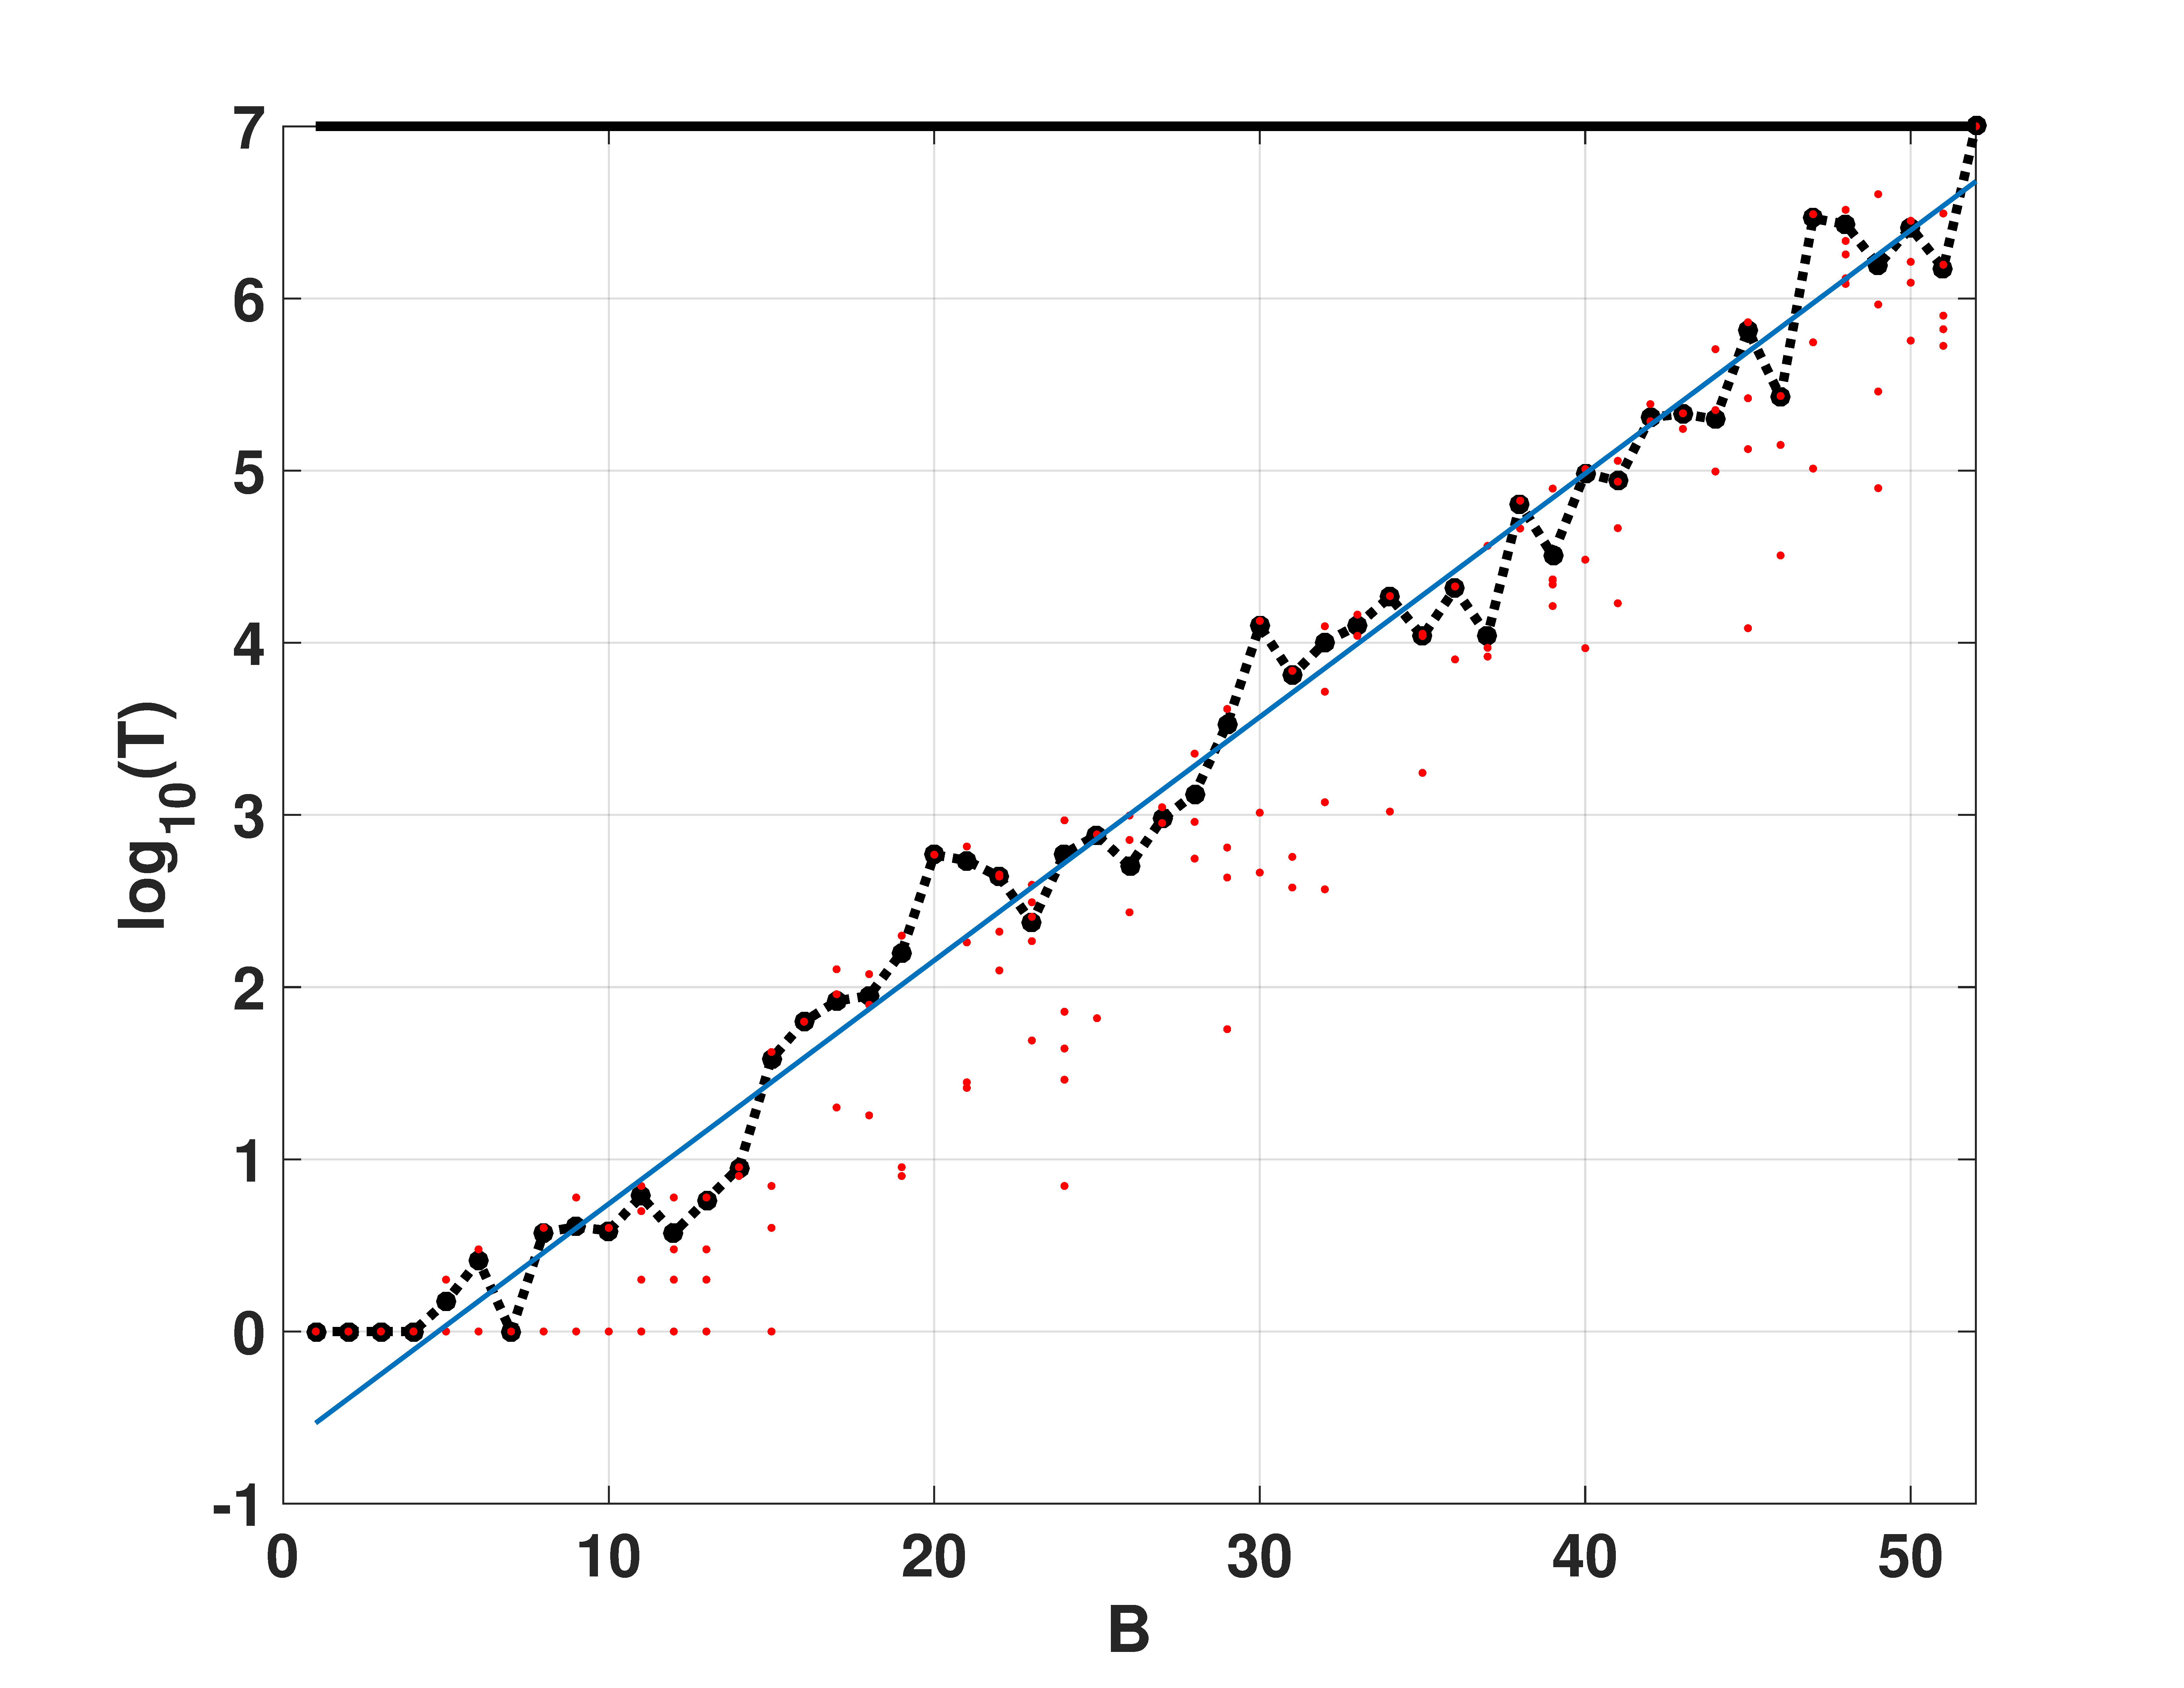
\includegraphics[width=.49\textwidth]{Period_Log}
	\caption{Period as function of precision in binary digits (see text).}
	\label{fig:period}
\end{figure}

\begin{table}[H]
\centering	
	\caption{Period $T$ as a function of $B$ for the maps considered}
	\vspace{1em}
	\begin{tabular}{lll}
		\hline\noalign{\smallskip}
		map 	& m 	& b  \\
		\noalign{\smallskip}\hline\noalign{\smallskip}
		TENT	&0 		& 0 \\
		LOG 	&0.139 	& -0.6188 \\
		SWITCH 	&0.1462 & -0.5115 \\
		EVEN 	&0.1447 & -0.7783 \\
		ODD 	&0.1444 & -0.7683 \\
		\noalign{\smallskip}\hline
	\end{tabular}
	\label{tabla:periodos}	
\end{table}

Results are compatible for those obtained in \cite{Nagaraj2008}.
Switching between maps increases the period $T$ but skipping procedure decreases by almost half.

\subsection {Quantifiers of simple maps}\label{subsec:SimpleMaps}
Here we report our results for both simple maps, LOG and TENT

\subsubsection{Logistic map (LOG)} \label{subsubsec:log}

Logistic map is interesting because is representative of the very large family of quadratic maps.
Its expression is:
\begin{equation}\label{eq:logimap}
 x_{[n+1]}=4x_{[n]}(1-x_{[n]}) \,
\end{equation}
with $x_n\in\mathcal{R}$.

Note that to effectively work in a given representation it is necessary to change the expression of the map in order to make all the operations in the chosen representation numbers. For example, in the case of LOG the expression in binary fixed point numbers is:
\begin{equation}\label{eq:logimapB2}
x_{n+1}=4 \epsilon floor\{\frac{x_n(1-x_n)}{\epsilon}\} \,
\end{equation}
with $\epsilon = 2^B$ where $B$ is the number of bits that represents the fractional part.

According as B grows, statistical properties vary until they stabilize.
Figs. \ref{fig:LOG_QuantiB} (a) to (f) show the statistical properties of LOG map in floating point and fixed point representation.
All these figures show: $100$ red points for each fixed point precision ($B$) and in black their average (dashed black line connecting black dots), $100$ horizontal dashed blue lines that are the results of each run in floating point and a black solid line their average.
In this case, all the lines of the floating point are overlapped.

For $B\geq 30$ the value of $H_{val}$ remains almost identical to the values for the floating point representation whereas $H_{BP}$ and $C_{BP}$ stabilizes at $B>21$.
Their values are: $<H_{val}>=0.9669$; $<H_{BP}>=0.6269$; $<C_{BP}>=0.4843$.
Note that the stable value of missing patterns $MP=645$ makes the optimum $H_{BP} \leq ln(75)/ln(720) \simeq 0.65$.
Then, $B=30$ is the most convenient choice because an increase in the number of fractional digits does not improve the statistical properties.

Some conclusions can be drawn regarding \textit{BP} and \textit{BPW} quantifiers.
For $B=1, 2, 3$ and $4$, the averaged $BP$ quantifiers are almost $0$ while the averaged $BPW$ quantifiers can not be calculated (seein Figs. \ref{fig:LOG_QuantiB} c and e the missing black dashed line).
For those sequences where the initial condition where $0$ all iterations result to be a sequence of $0$s (the fixed point of the map), this happens very likely with small precisions because of the roundoffs.

When $B$ increases, $B=7, 9$ and $12$, the used initial conditions are rounded to zero less frequently.
So the generated sequences start from some value but many of them fall to zero with a short transitory.
This can be seen in Figs. c and e, $BPW$ shows high dispersion unlike $BP$ quantifiers.
This is because $BPW$ procedure takes into account only the transient discarding fixed points, unlike $BP$ procedure that considers all the sequence. 
 
\textcolor{red}{ESTE PÁRRAFO VA A DESAPARECER CON LONG DOUBLE, O NO?, ADEMÁS DISTRAE DEL FOCO DEL TRABAJO. HAY QUE BUSCARLE UN LUGAR EN EL PAPER}
Finally, for $B = 45, 49, 51$ and $52$ some $BP$ quantifiers have a low value, but $BPW$ quantifiers have a more predictible behavior, we can see that these atractors fall to a fixed point with a long transitory.
In this behaviour is due to the employed plataform.
The operation miltiplication needs the double of bits to be represented but the machine has only $64$.
Acá lo que quiero decir es que en las figuras \ref{fig:LOG_QuantiB} a, b y d las corridas con punto fijo tienen alta dispersión y aparecen algunas con valores muy bajos.
Esto es por que la aritmética de punto fijo la estamos queriendo generar artificialmente con una variable de tipo double que tiene una mantisa de 53 bits.
Entonces en la multiplicación (que duplica la cantidad de bits necesarios) se pierden muchos fraccionarios.
Lo mismo pasa si se usa el tipo float, que tiene 27 bits de mantisa pero mucho antes, a partir de B>24+-.
Con long double debería desaparecer.
Entonces hay que tener en cuenta esto cuando se simula punto fijo con la computadora, en los mapas que halla multiplicaciones.

\begin{figure}
	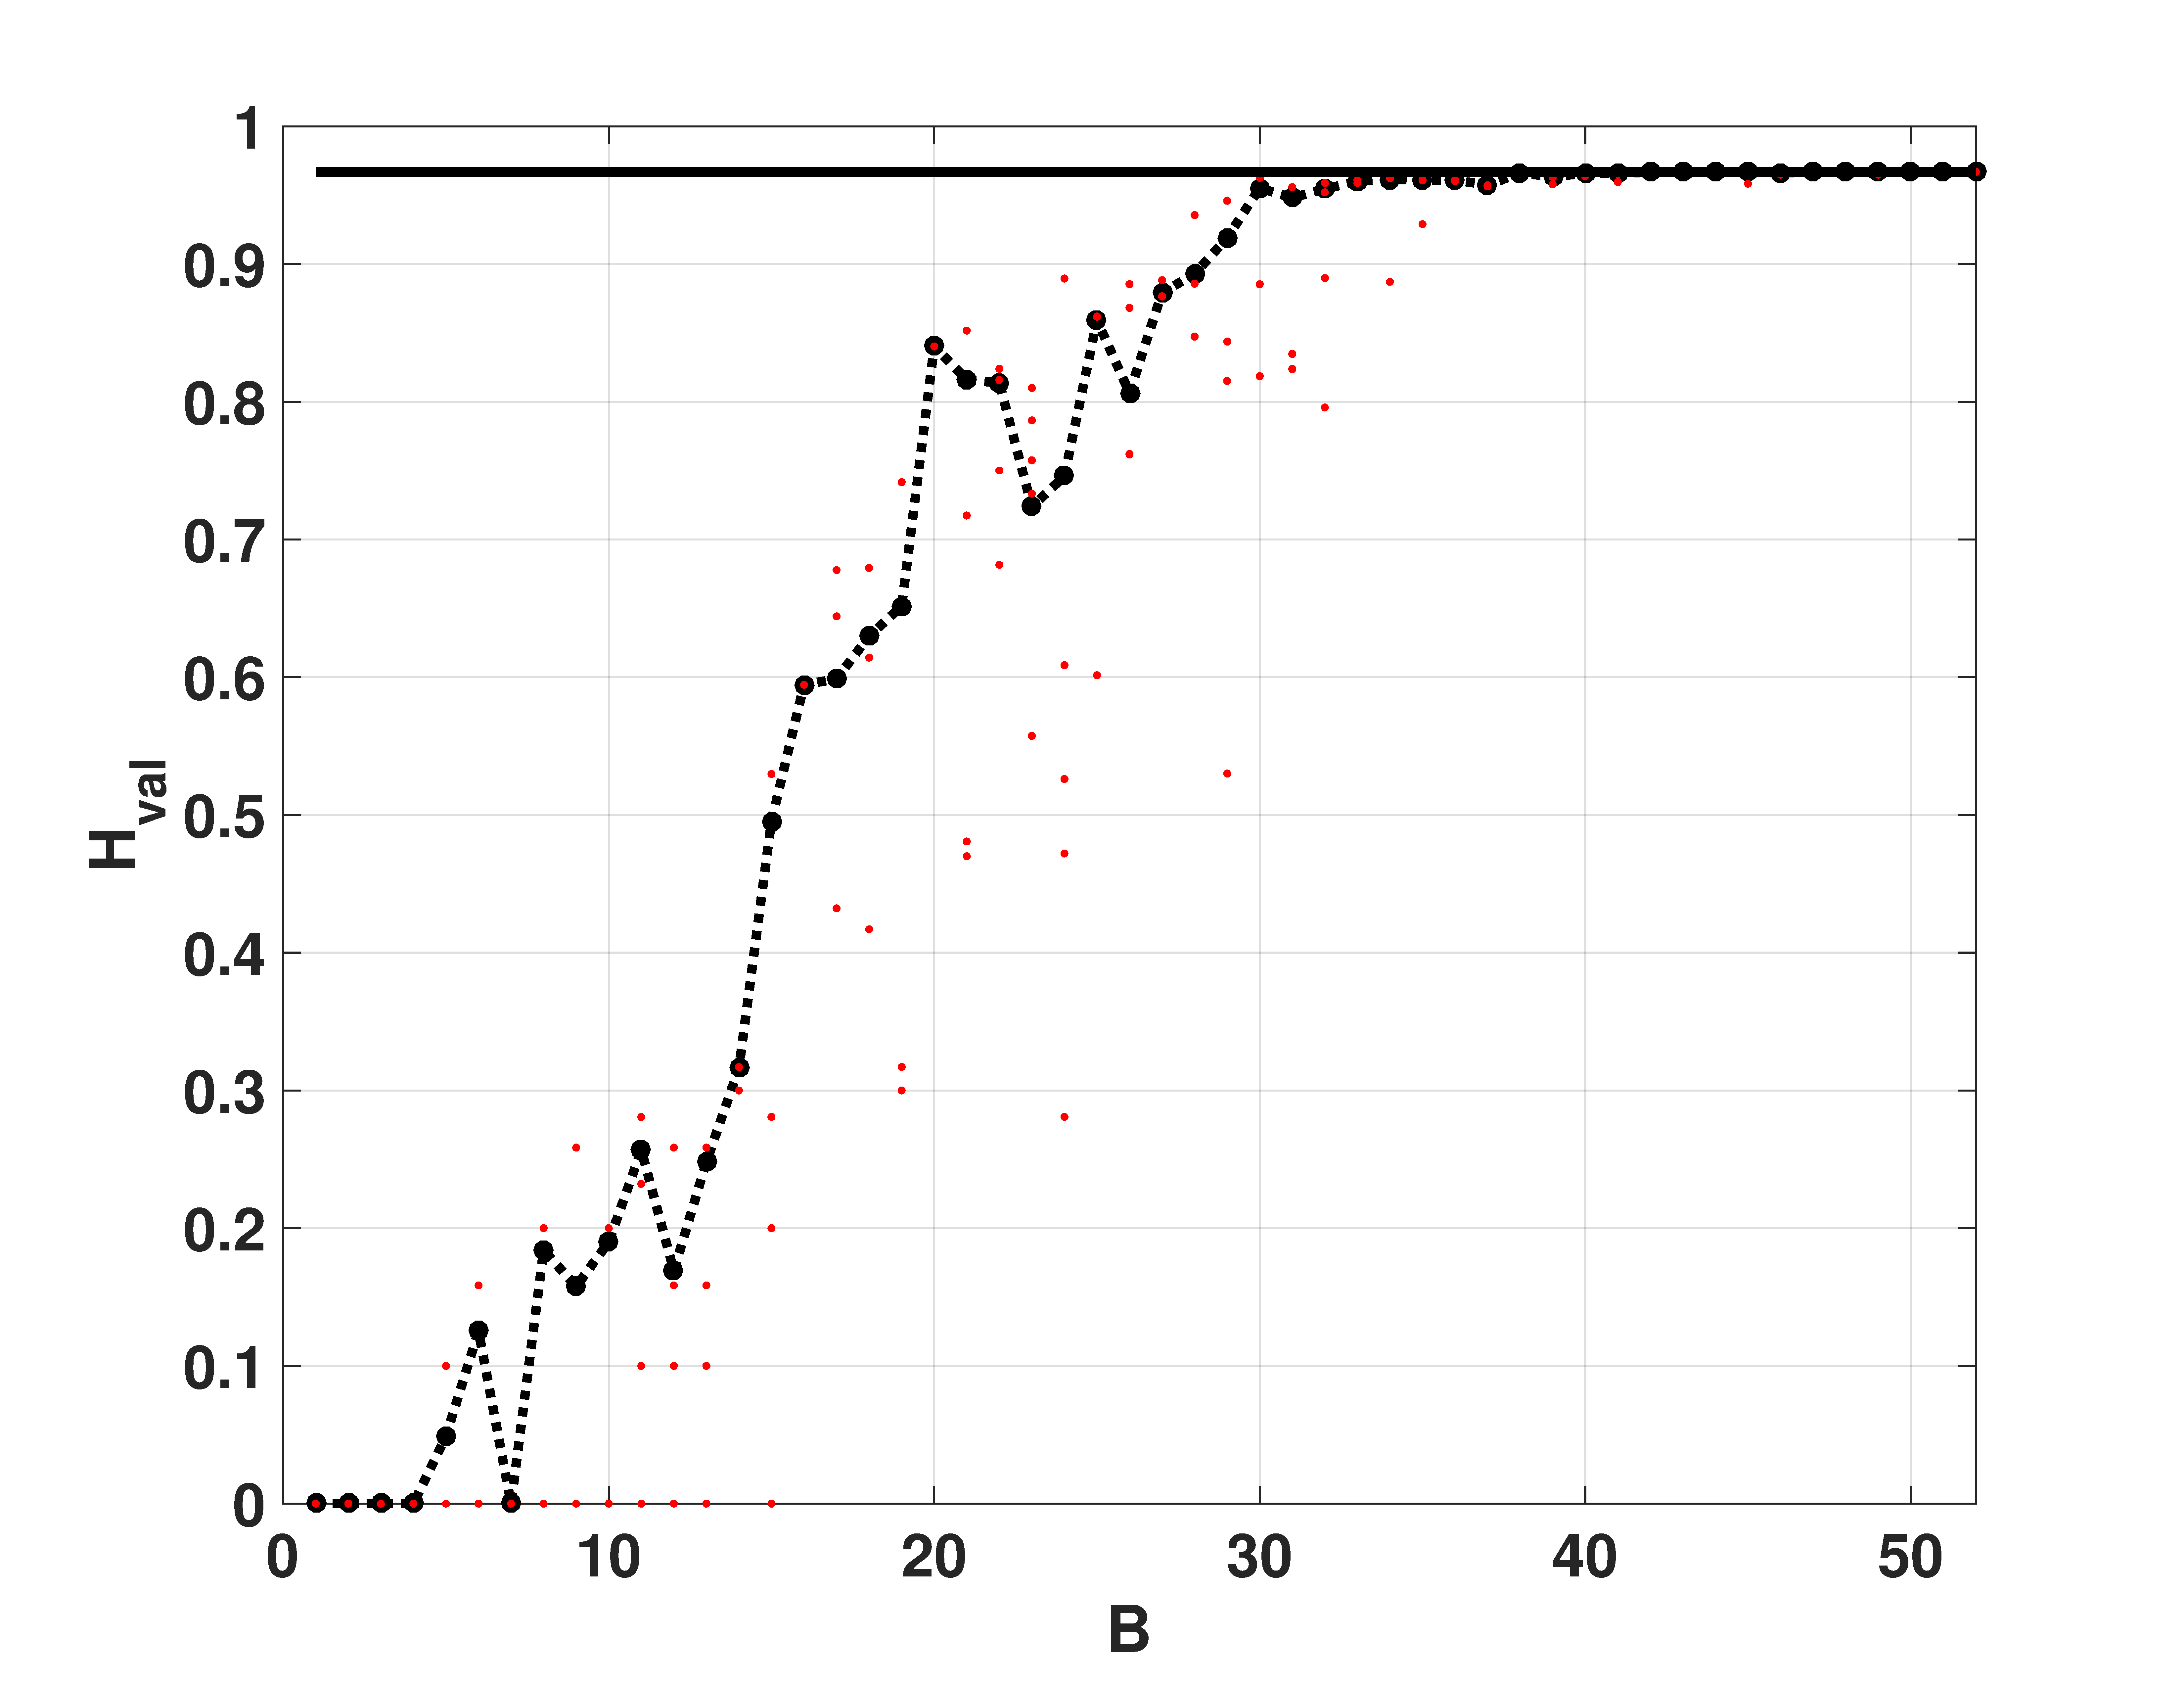
\includegraphics[width= .49\textwidth]{Hval_Log}
	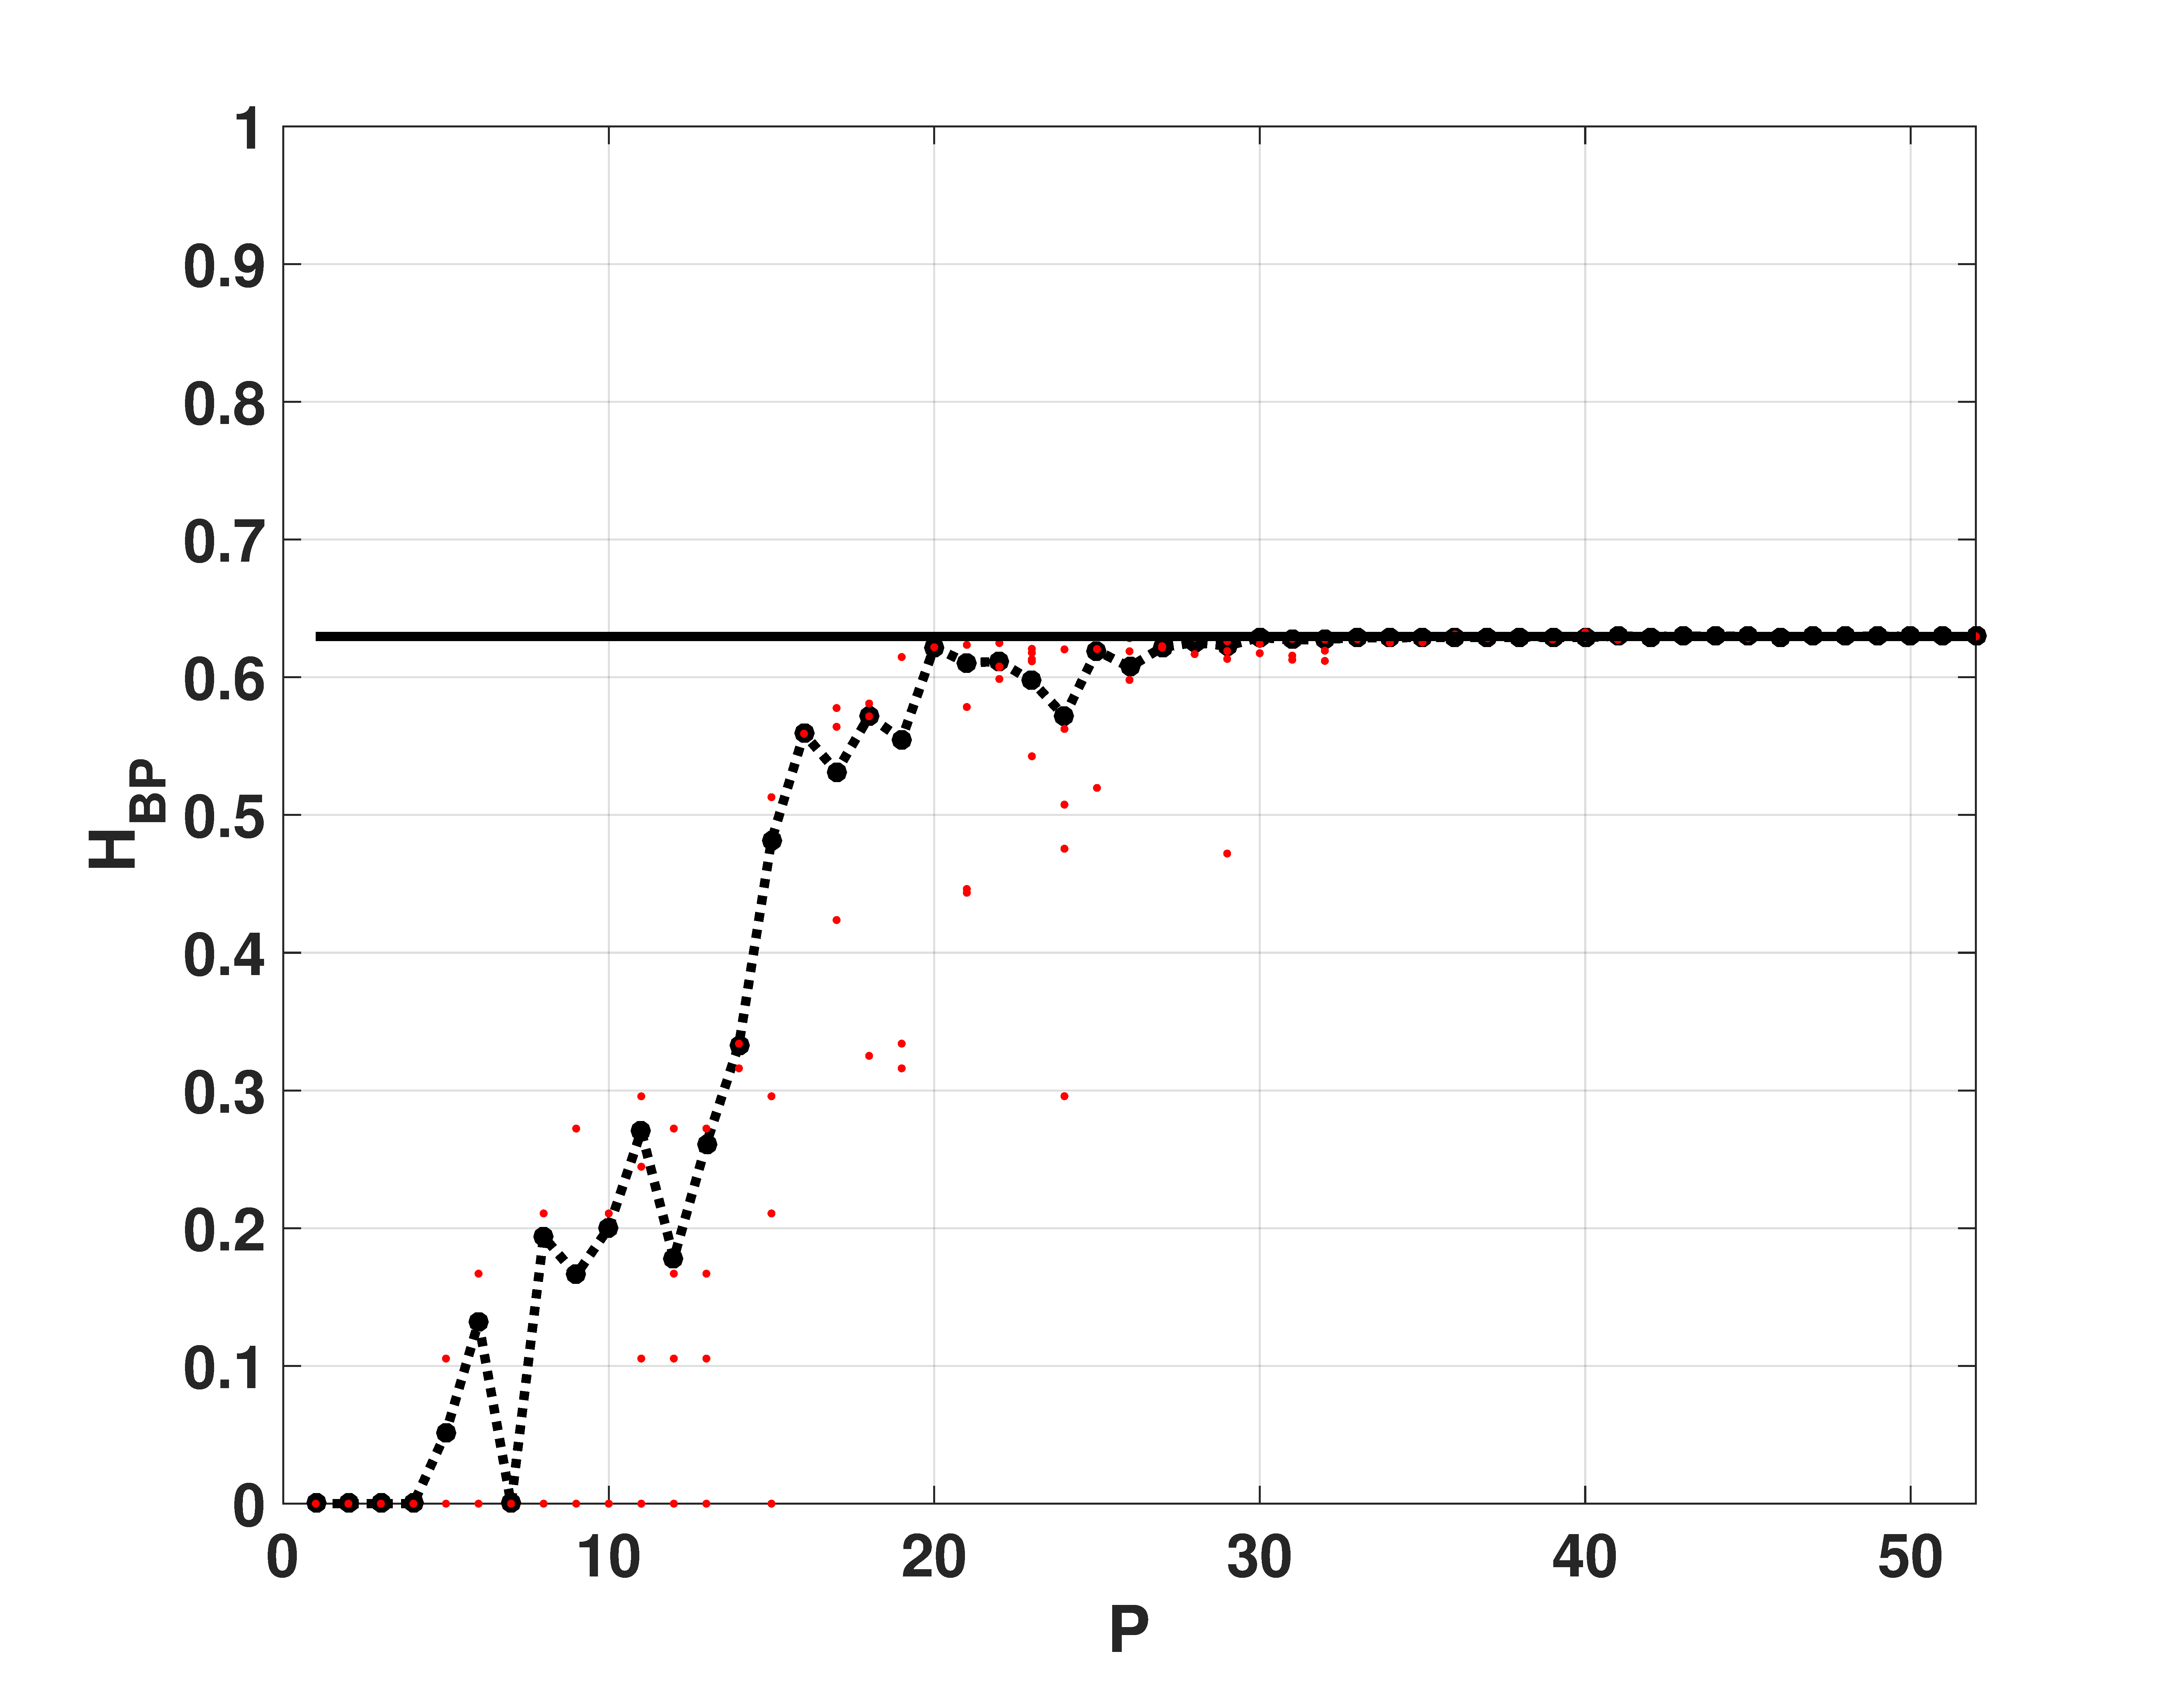
\includegraphics[width= .49\textwidth]{Hbp_Log}
	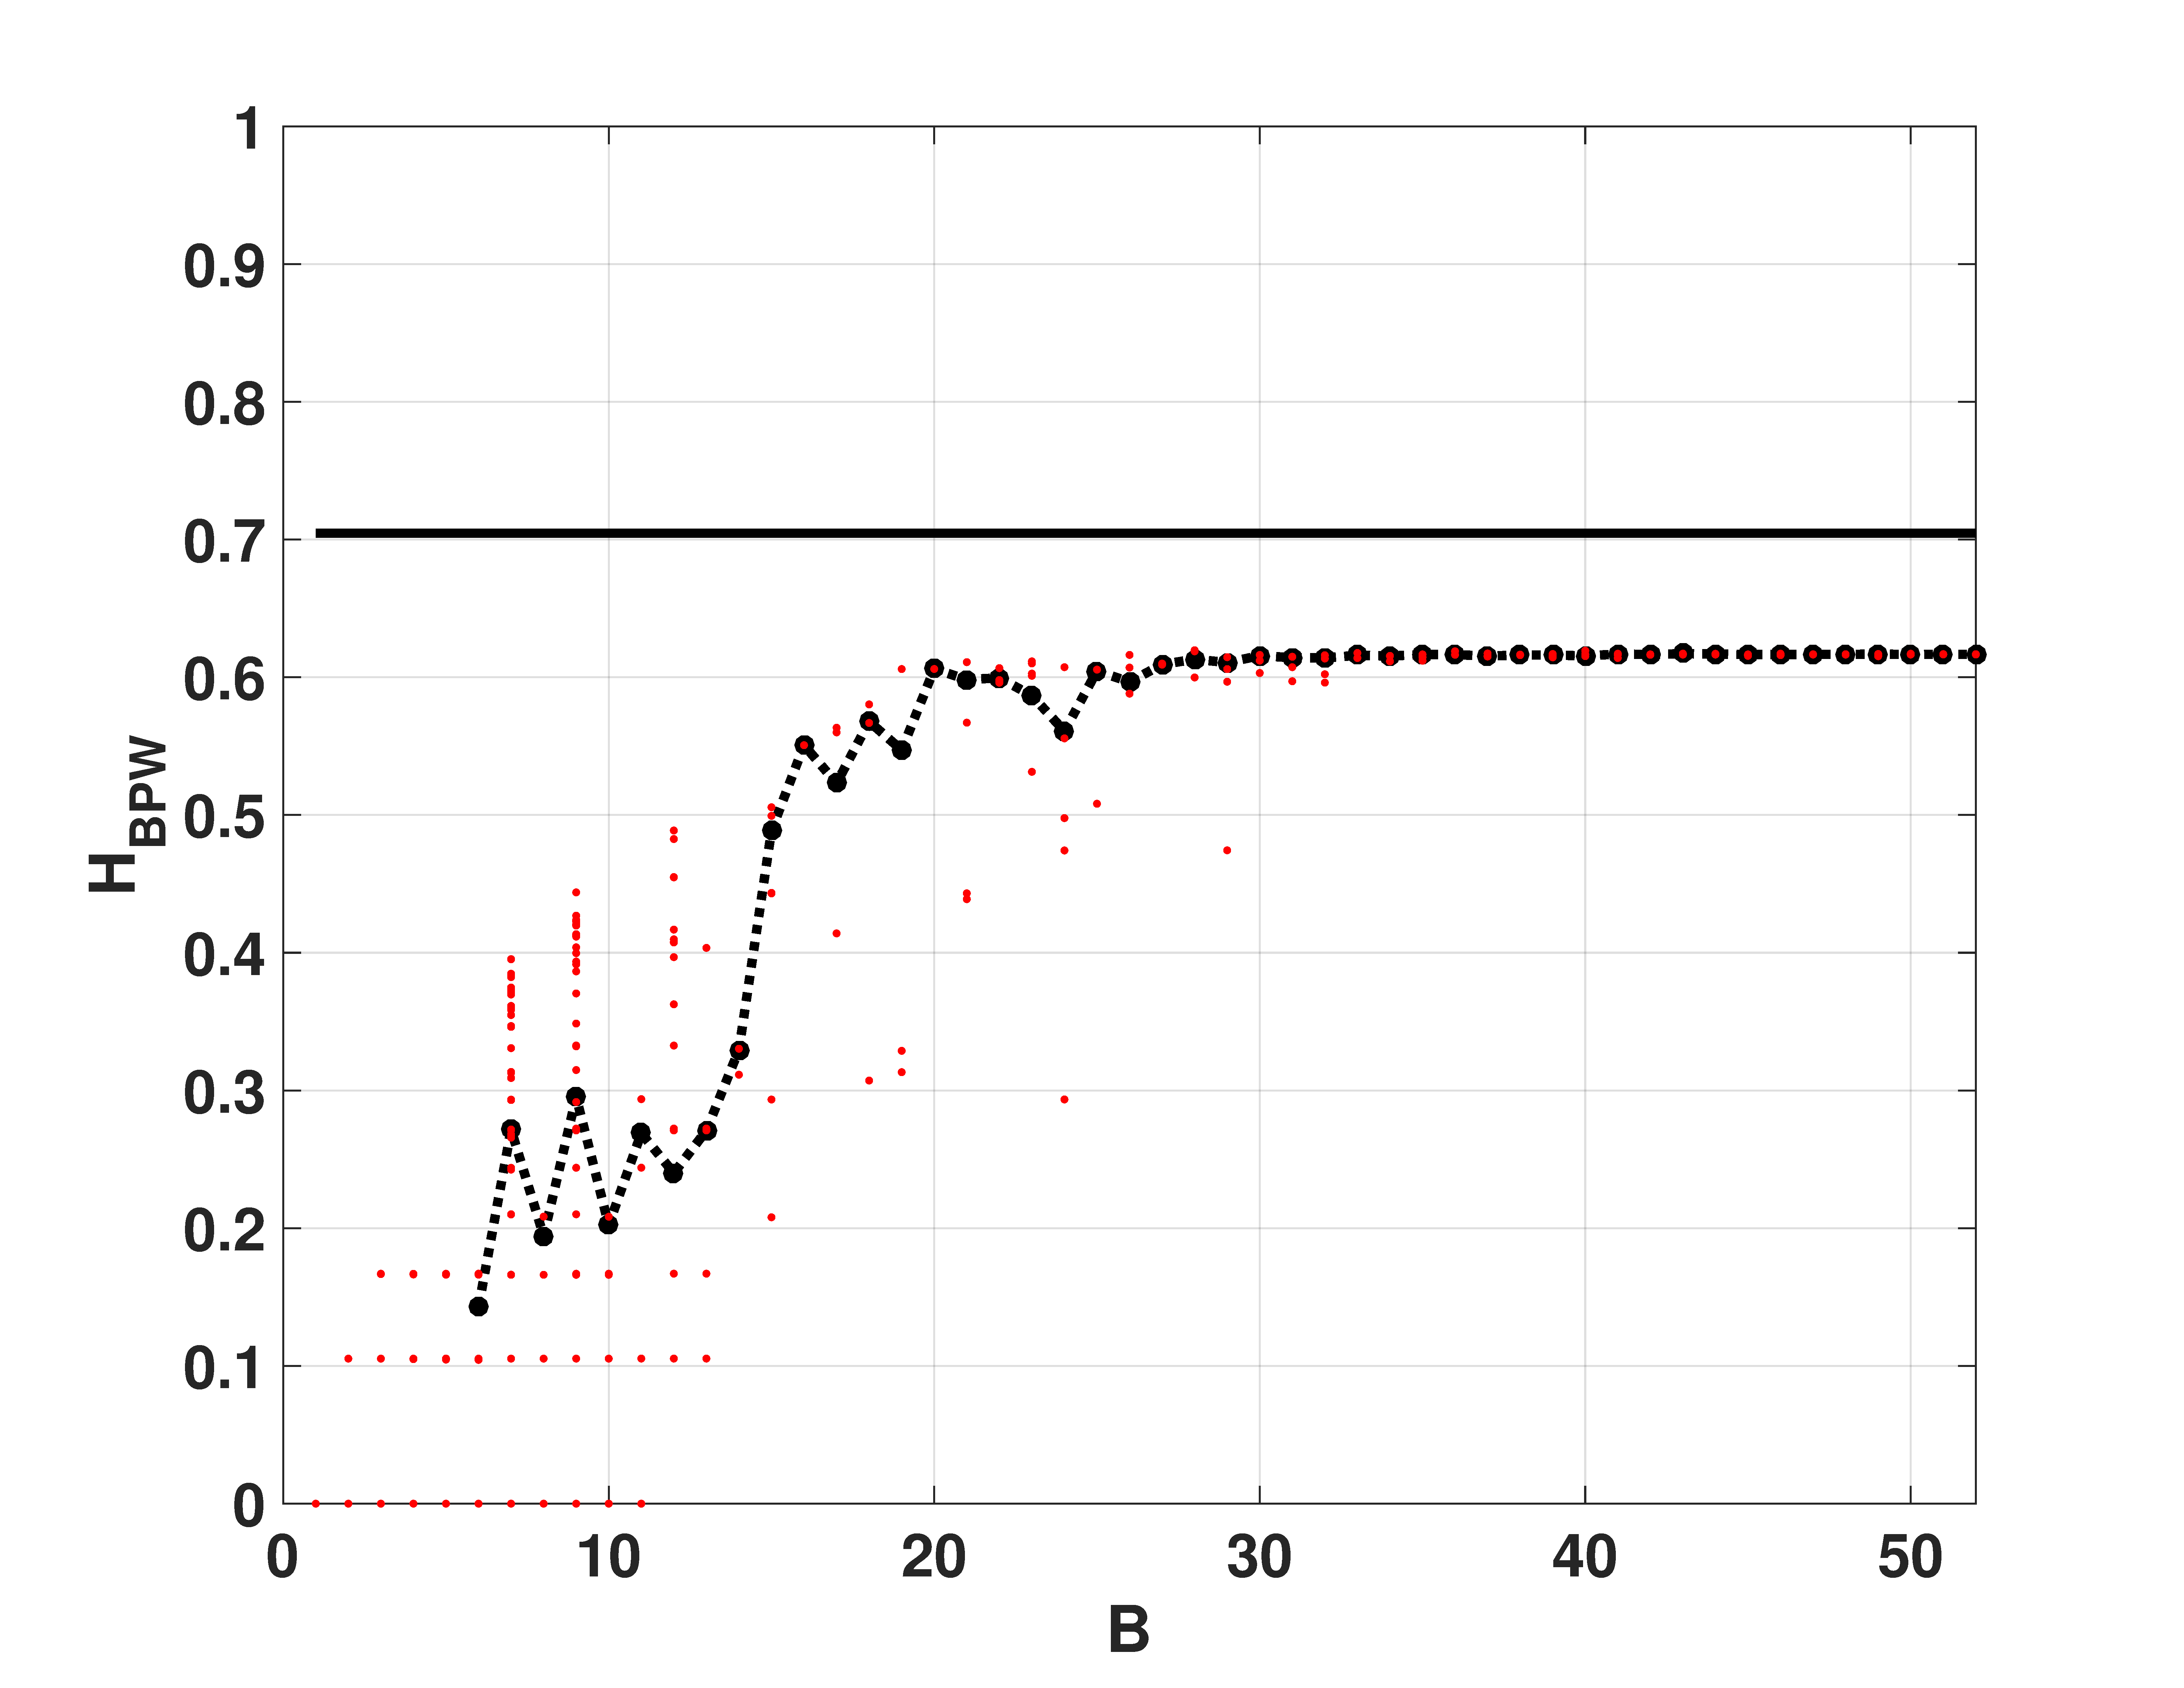
\includegraphics[width= .49\textwidth]{Hbpw_Log}
	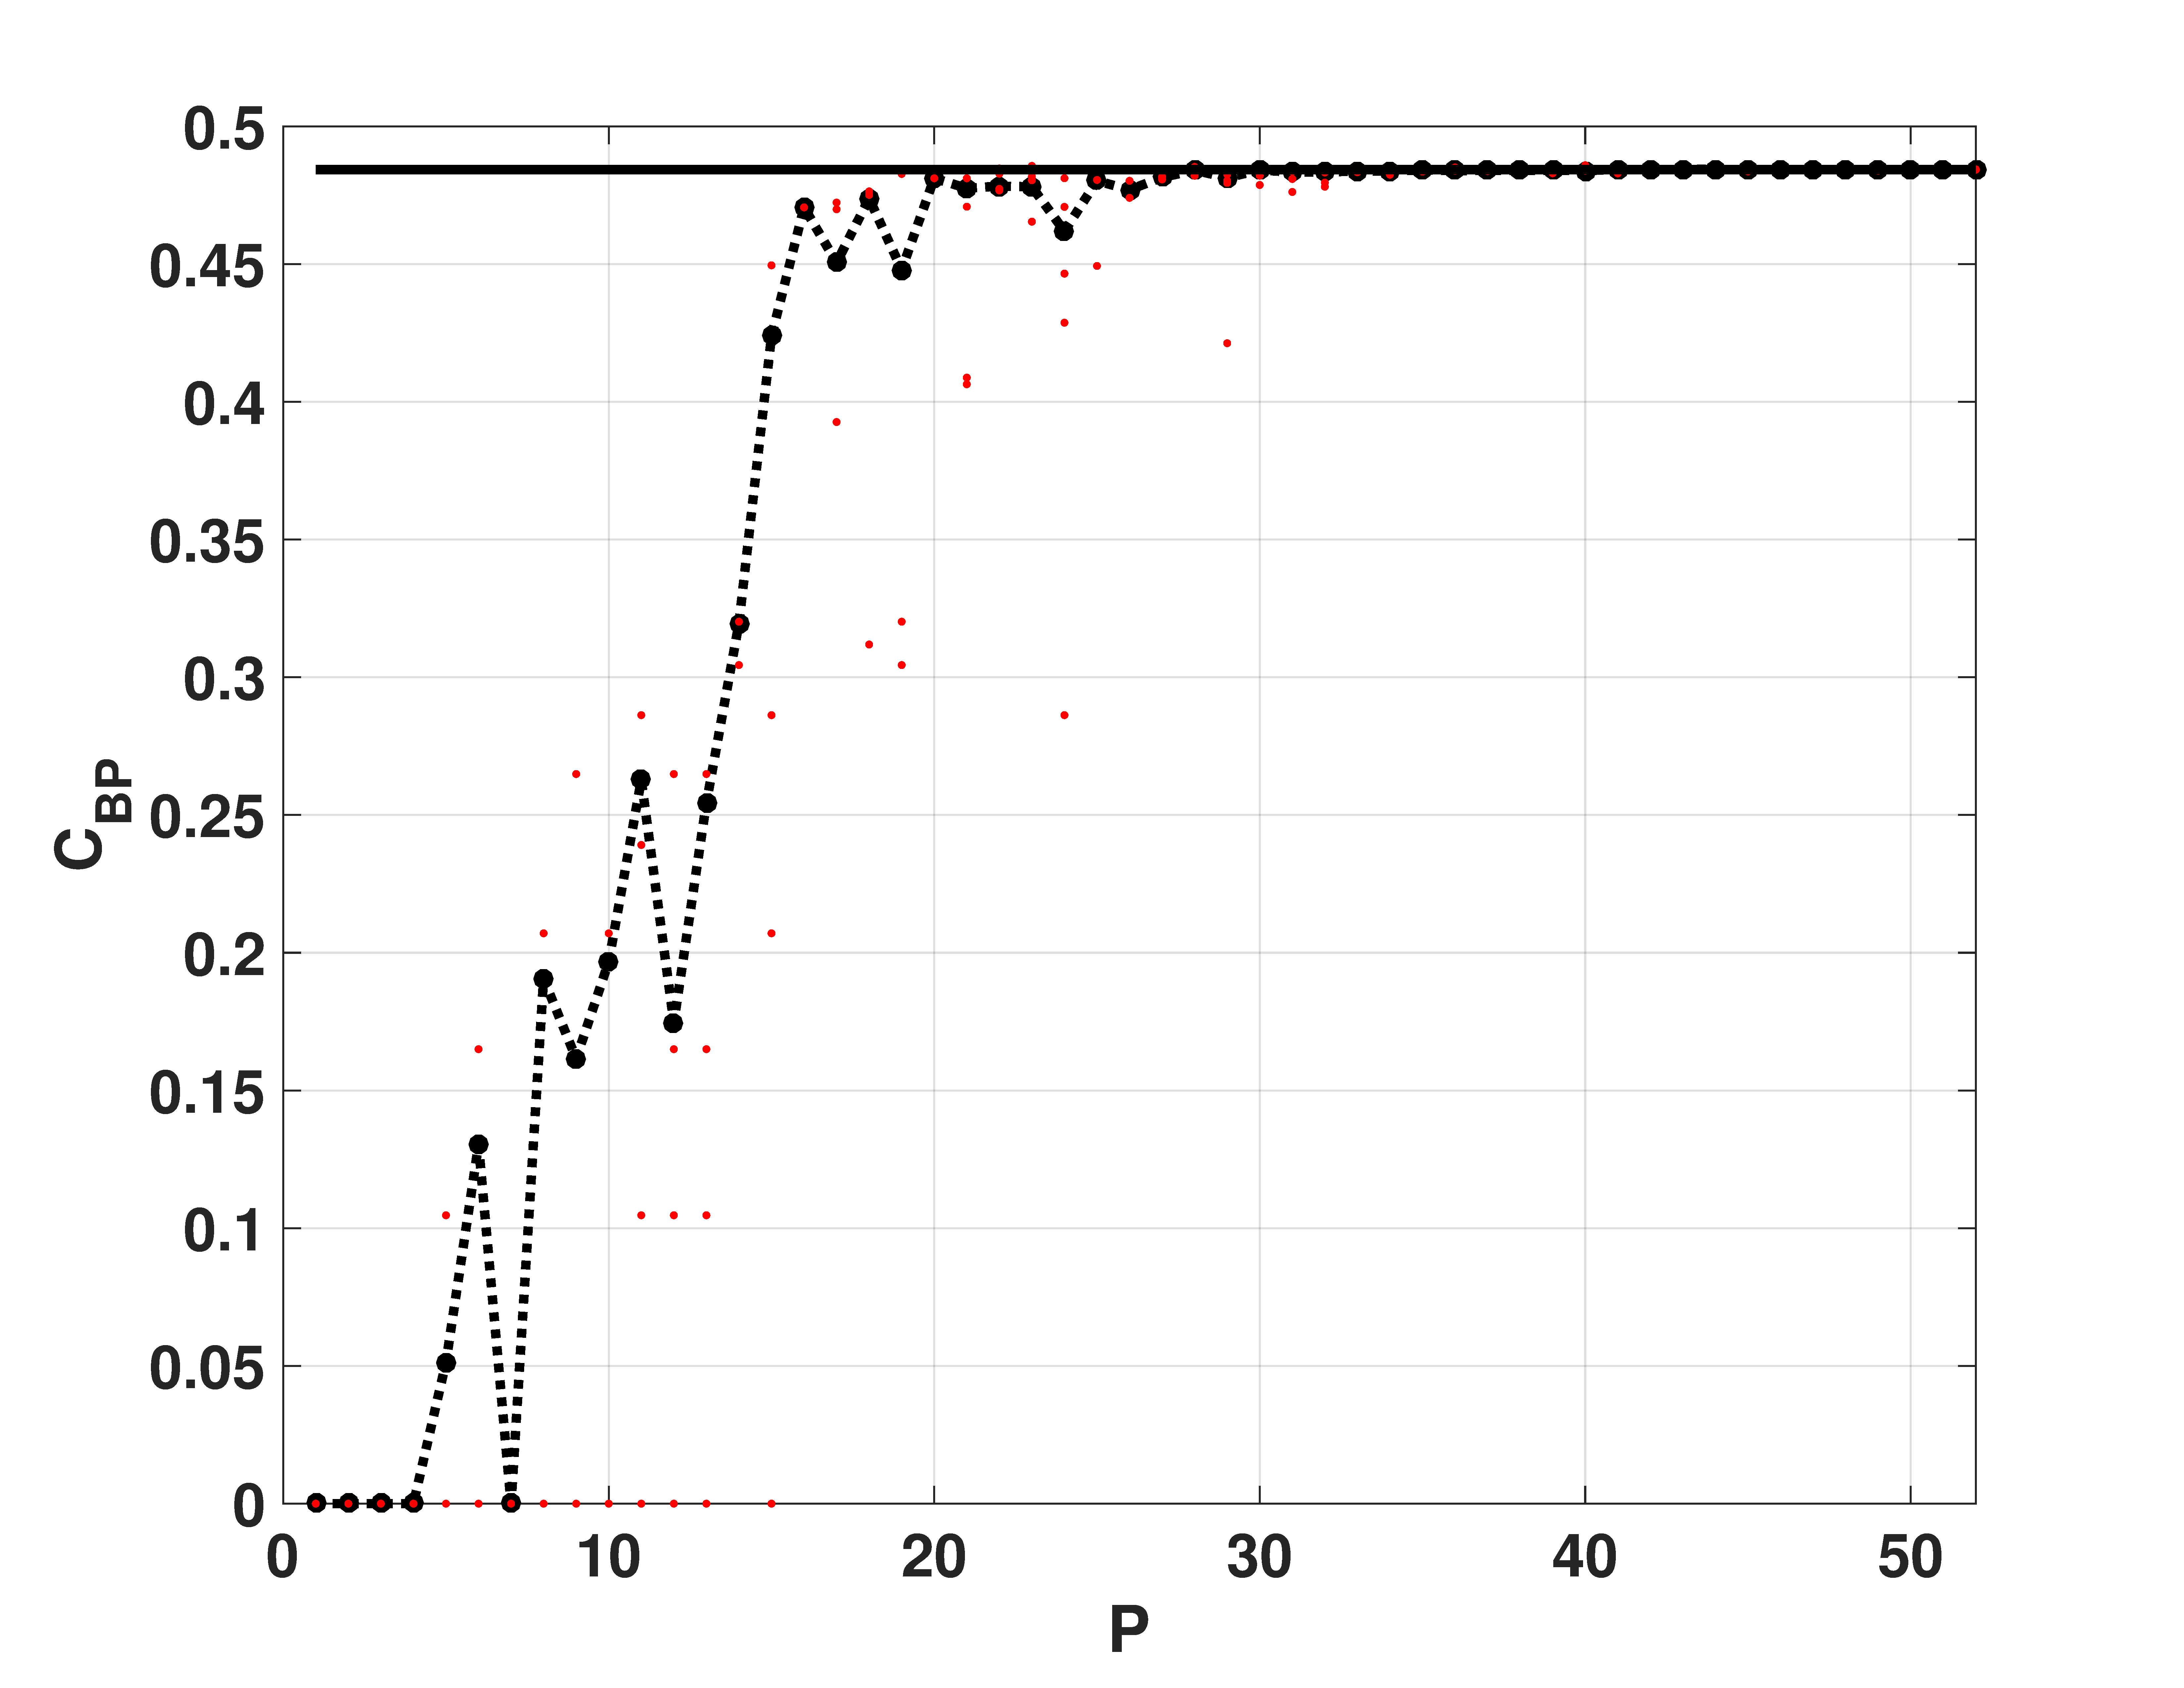
\includegraphics[width= .49\textwidth]{Cbp_Log}
	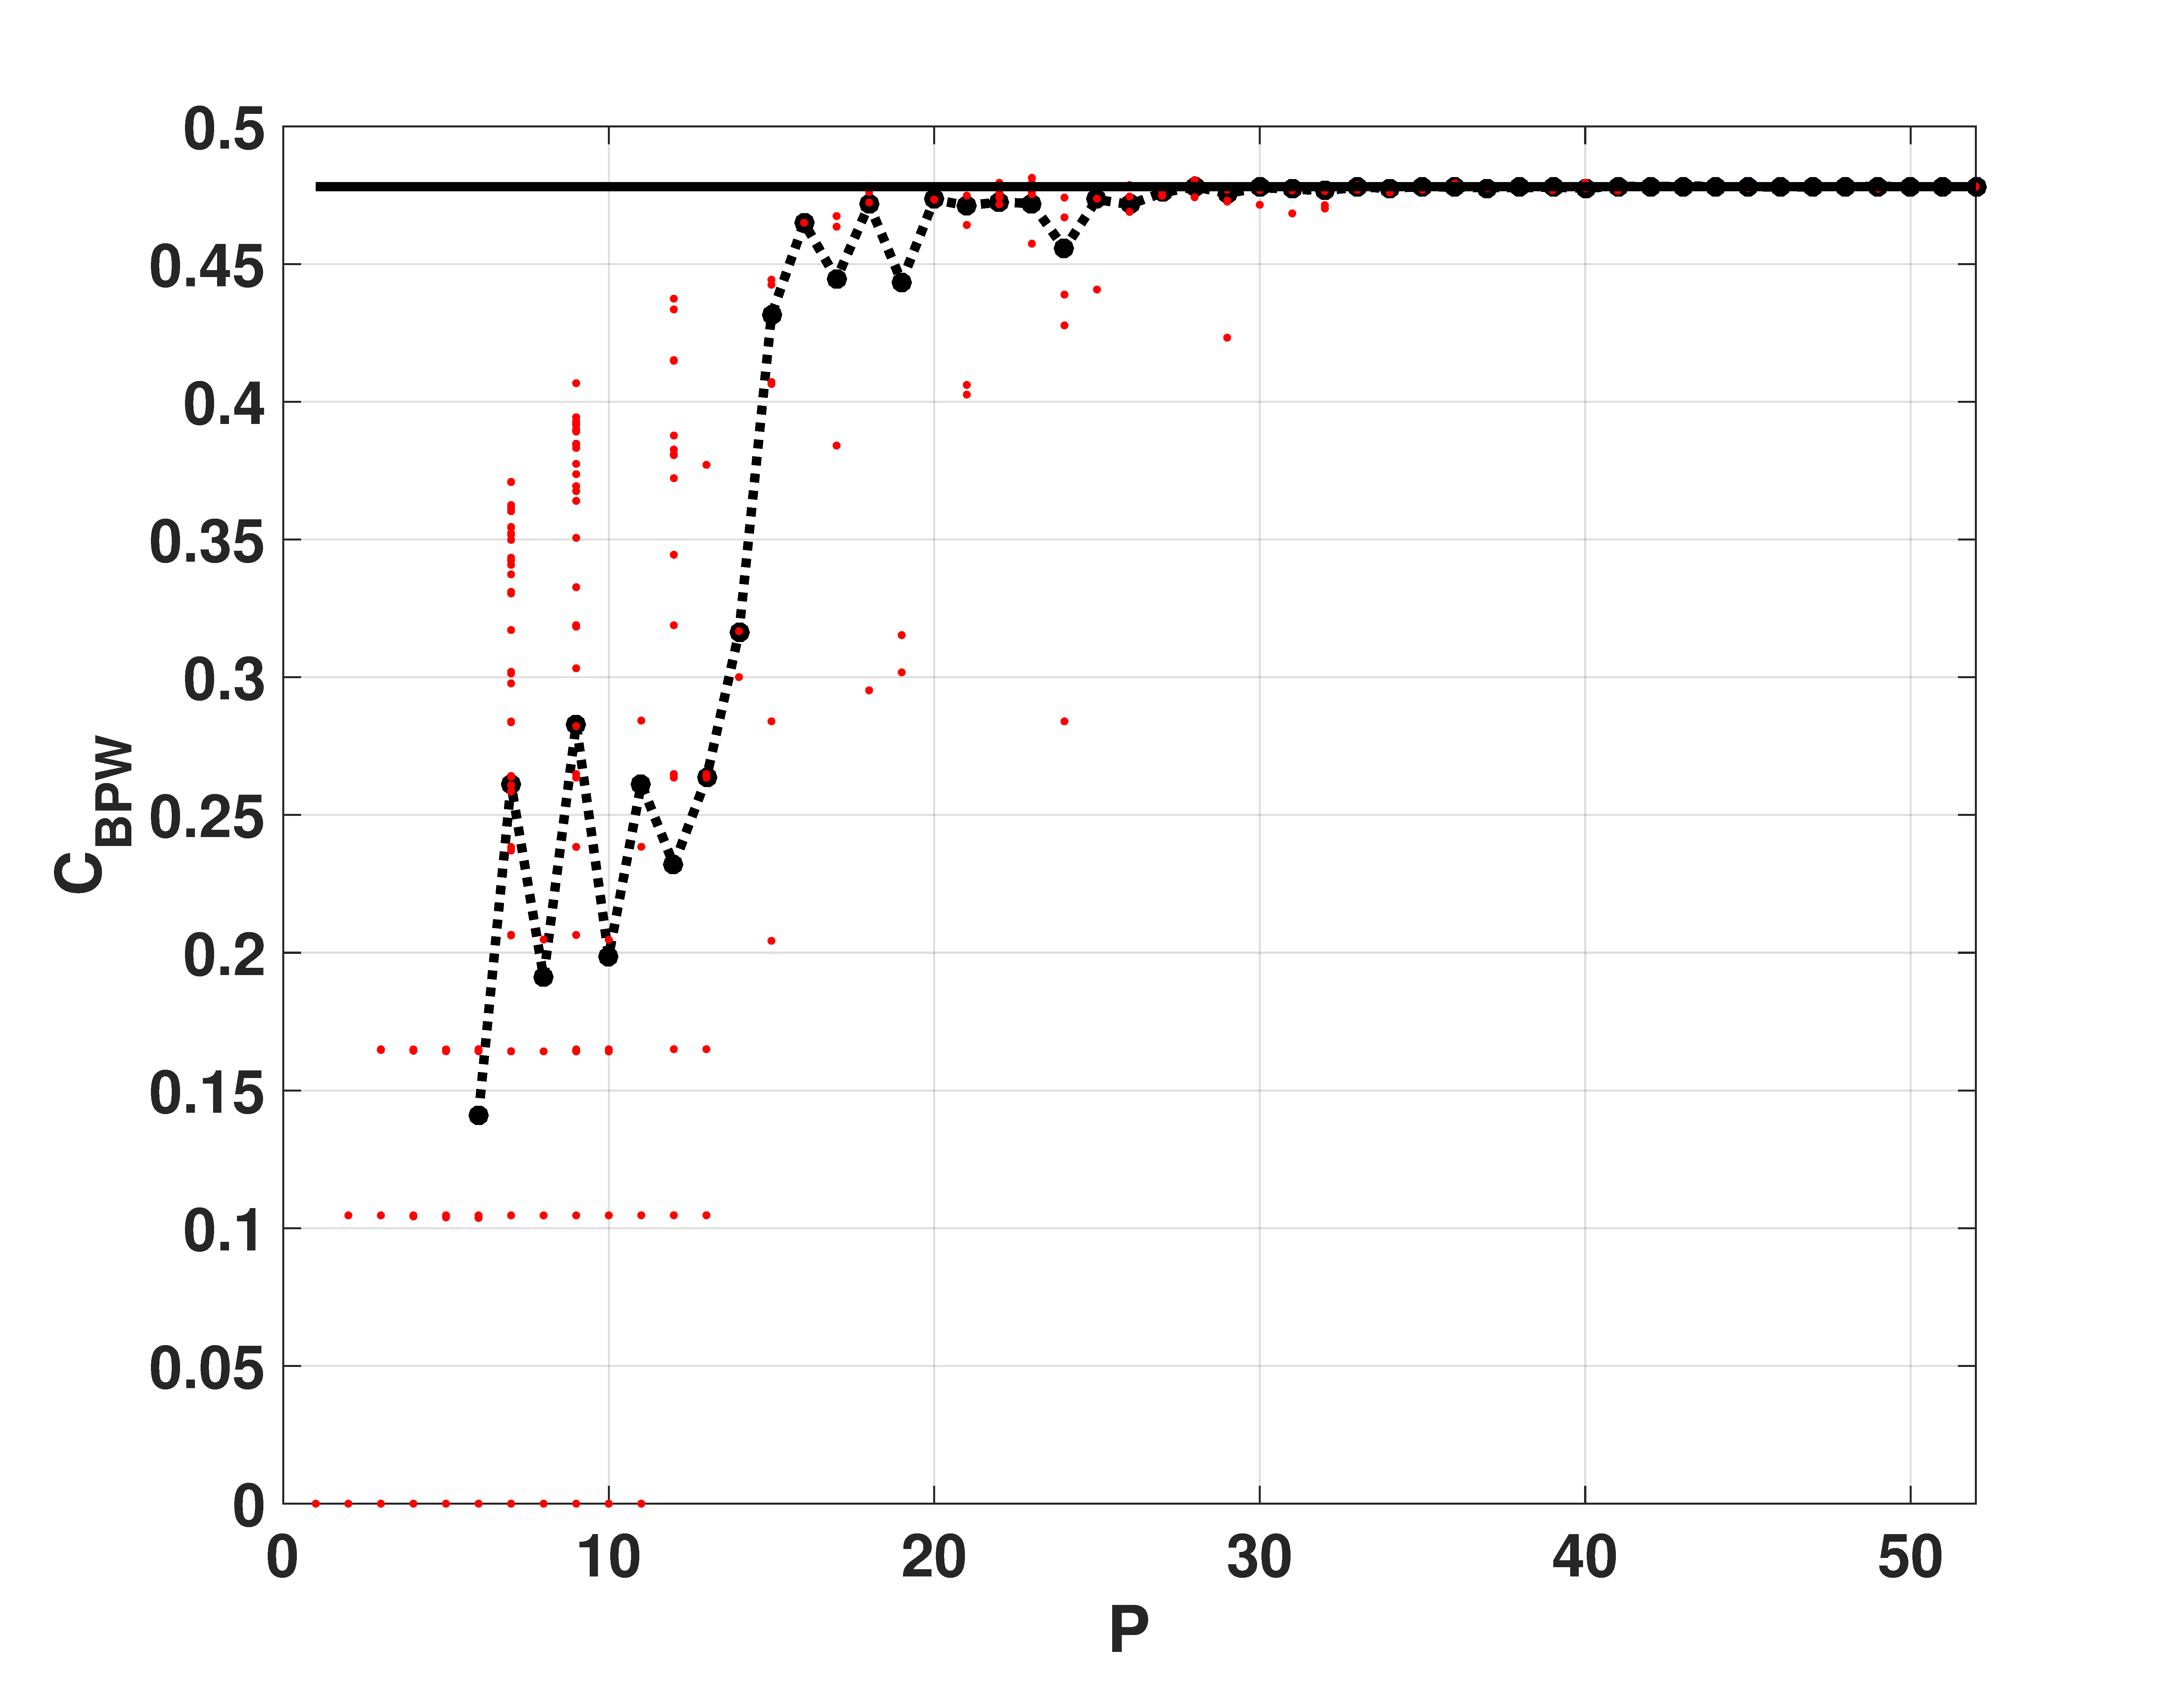
\includegraphics[width= .49\textwidth]{Cbpw_Log}
	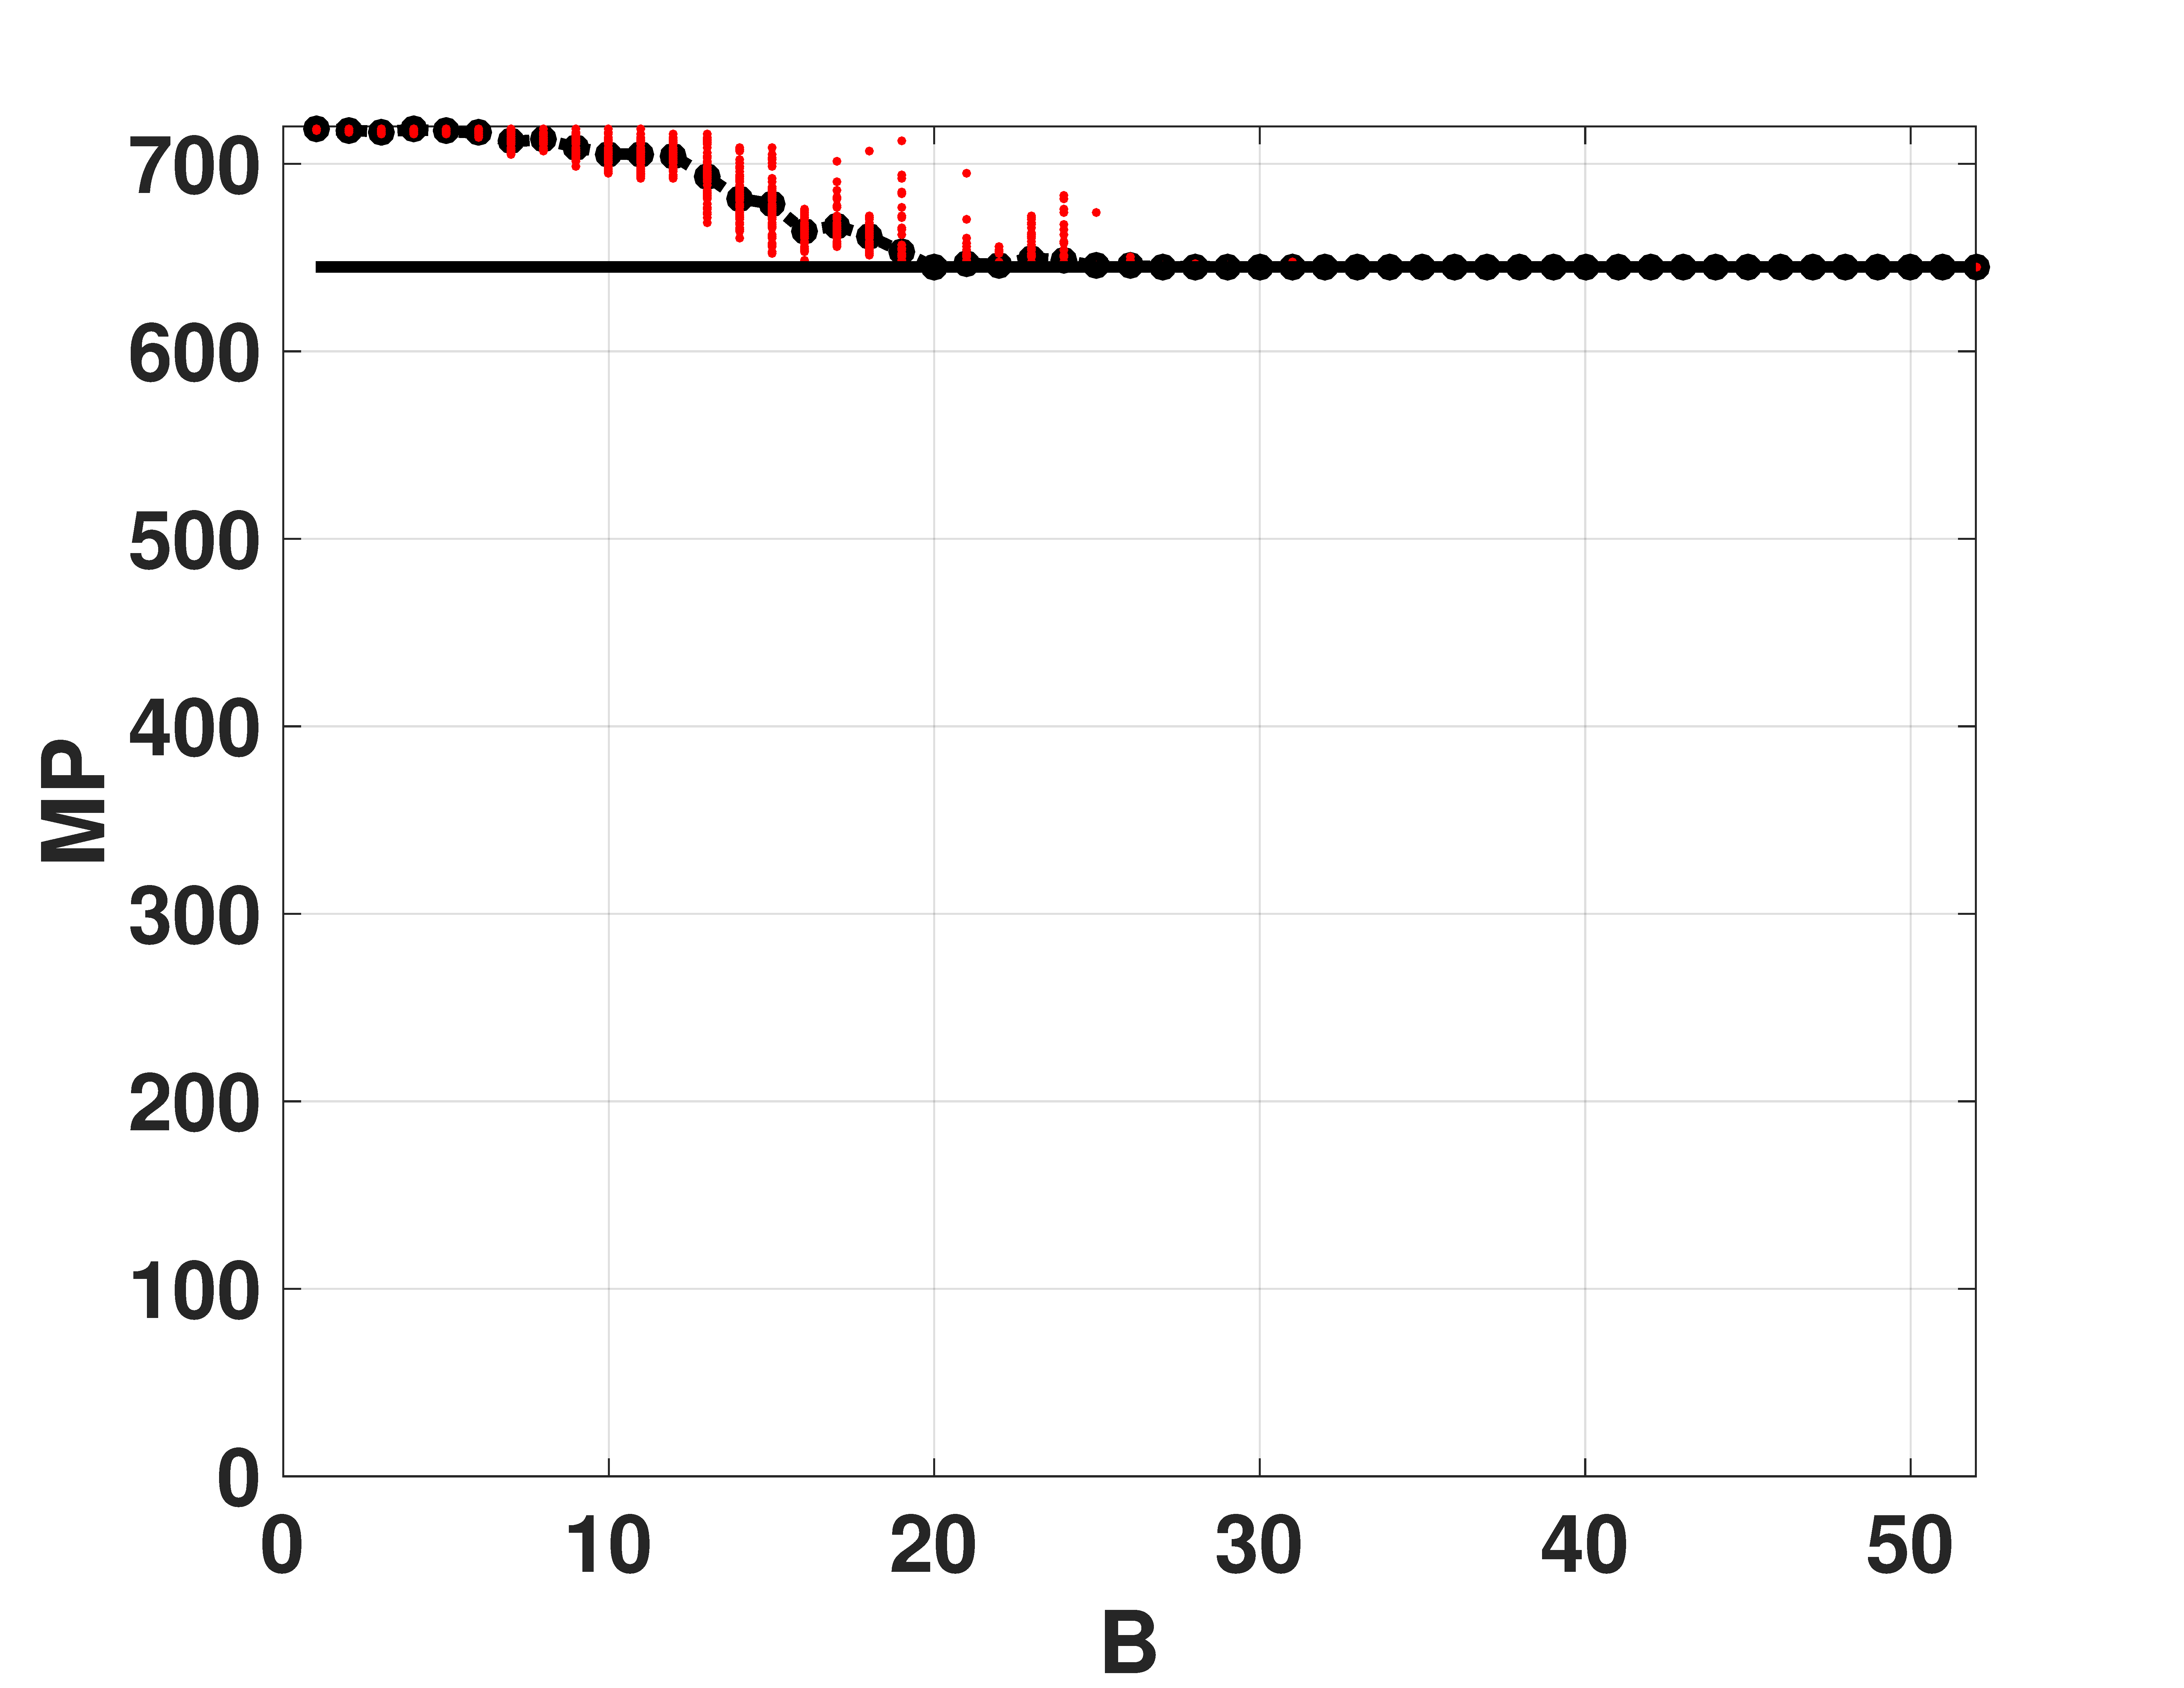
\includegraphics[width= .49\textwidth]{MP_Log}
	\caption{Statistical properties of the LOG map: (a) $H_{val}$ vs $B$ (b) $H_{BP}$ vs $B$ (c) $C_{BP}$ vs $B$ (d) $MP$ vs $B$.}
	\label{fig:LOG_QuantiB}
\end{figure}

The same results are now shown in double entropy planes with the precision as parameter (Fig. \ref{fig:LOG_HH}).
These figures show: $100$ red points for each fixed point precision ($B$) and in black their average (dashed black line connecting black dots), $100$ blue dots that are the results of each run in floating point and a black star their average.
This last $100$ points and their average are overlapped.

As expected, the fixed point architecture implementation converges to the floating point value as $B$ increases.
For both, Hbp-Hval and Hbpw-Hval, from $B=20$, $H_{val}$ improves but $H_{BP}$ remains constant.
It can be seen that the distribution of values reaches high values ($<H_{val}>=0.9669$) but their mixing is poor ($<H_{BP}>=0.6269$).

\begin{figure}
	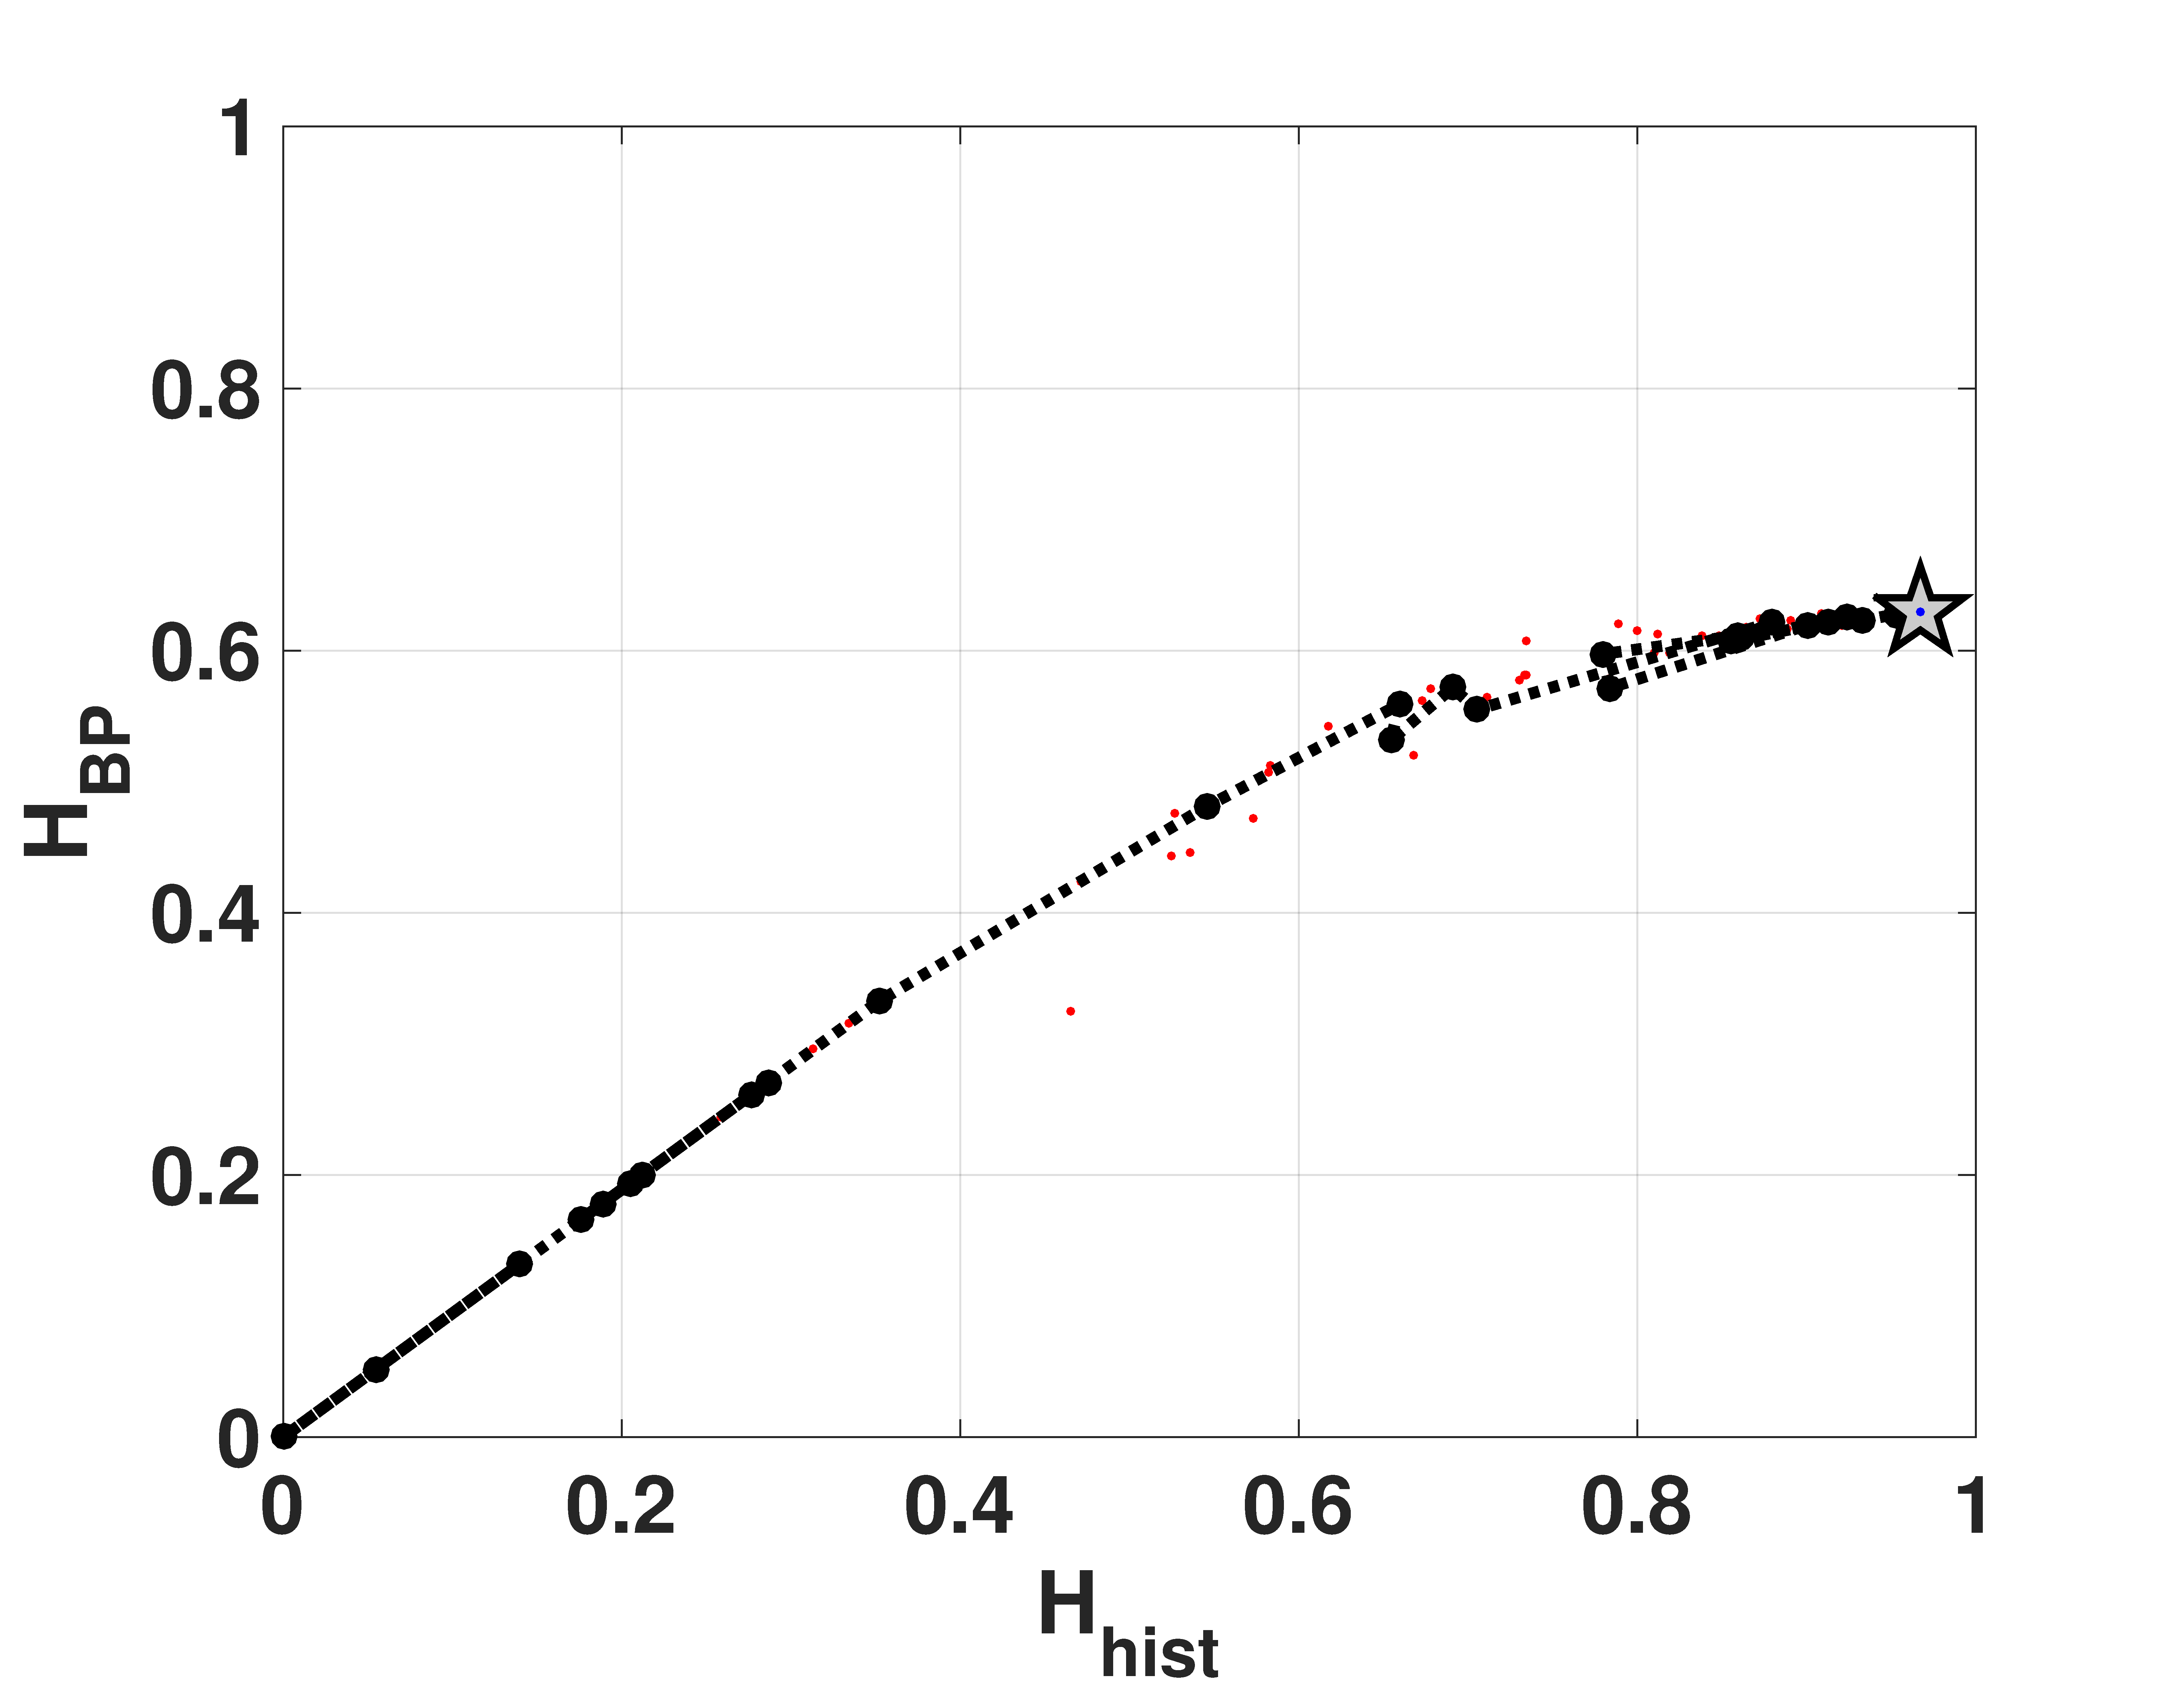
\includegraphics[width= .49\textwidth]{HbpHval_Log}
	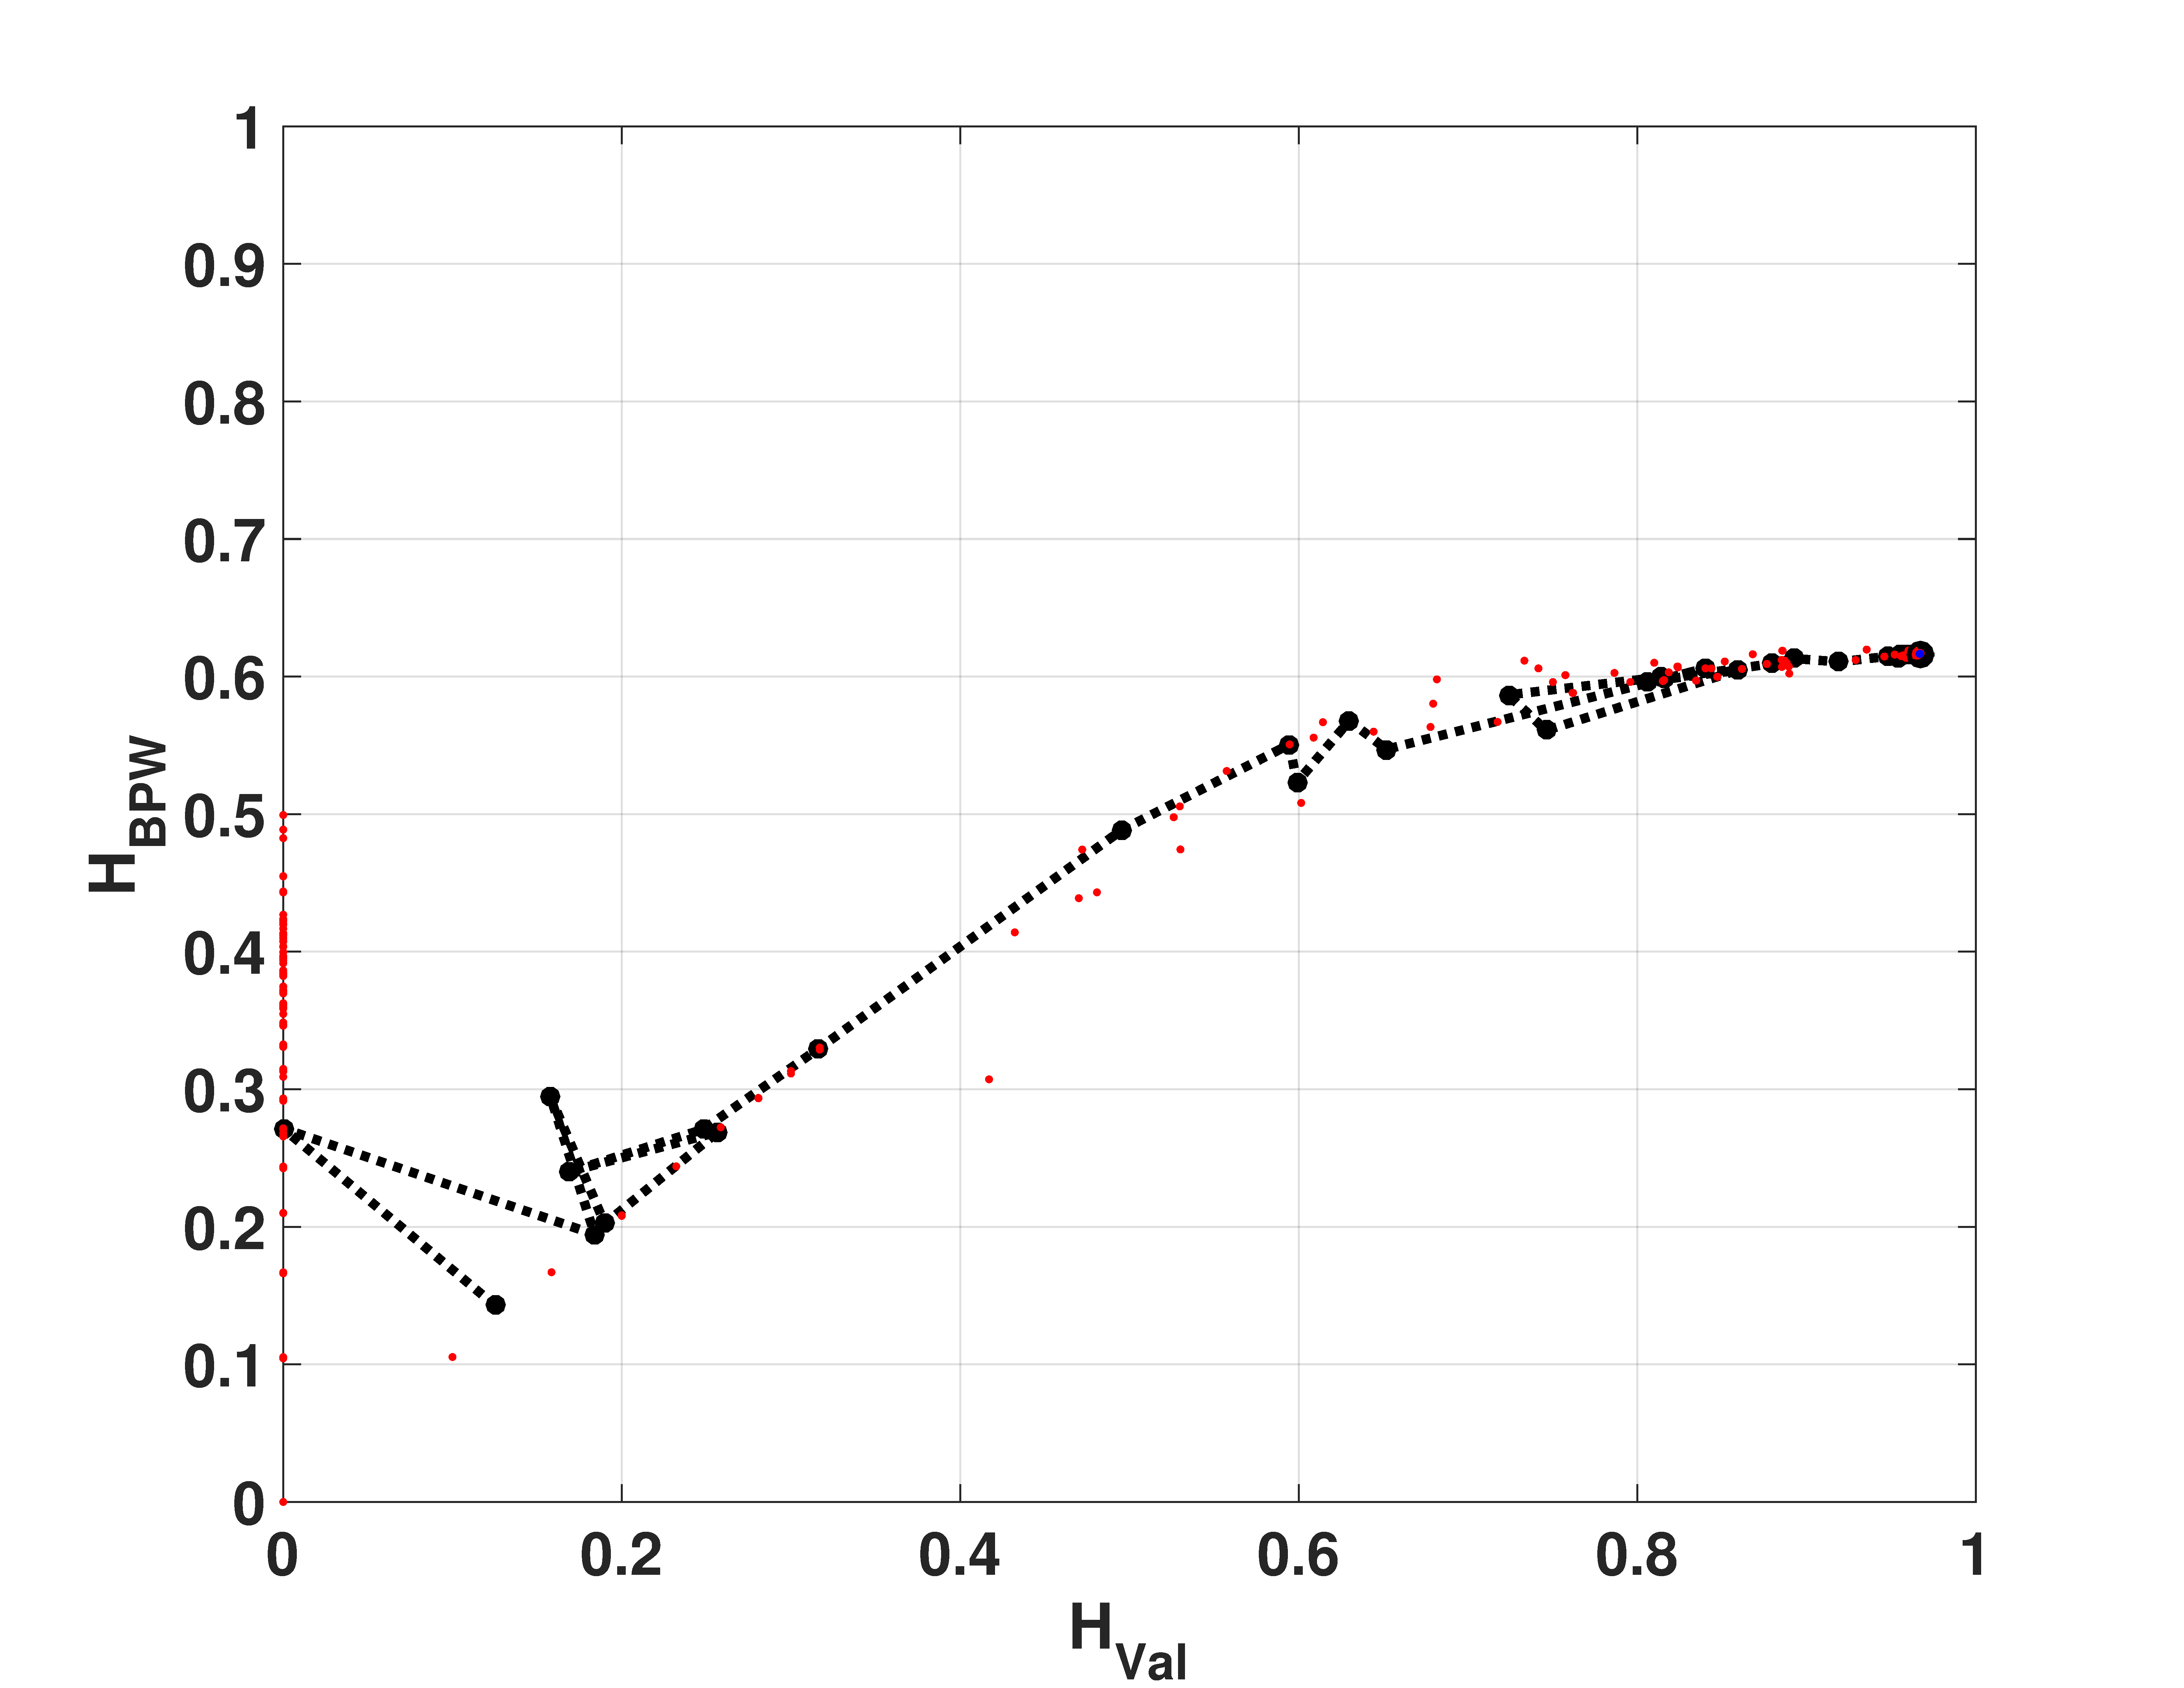
\includegraphics[width= .49\textwidth]{HbpwHval_Log}
	\caption{Evolution of statistical properties in double entropy plane of LOG map: (a) $H_{val}$ vs $H_{BP}$ (b) $H_{val}$ vs $H_{BPW}$.}
	\label{fig:LOG_HH}
\end{figure}

In Fig. \ref{fig:LOG_HC} we show the entropy-complexity planes.
Dotted gray lines are the upper and lower margins, is expected that a chaotic system remains near the upper margin.
These results characterize a chaotic behaviour, in $H_{BP}-C_{BP}$ plane we can see a low entropy and high complexity.

\begin{figure}
	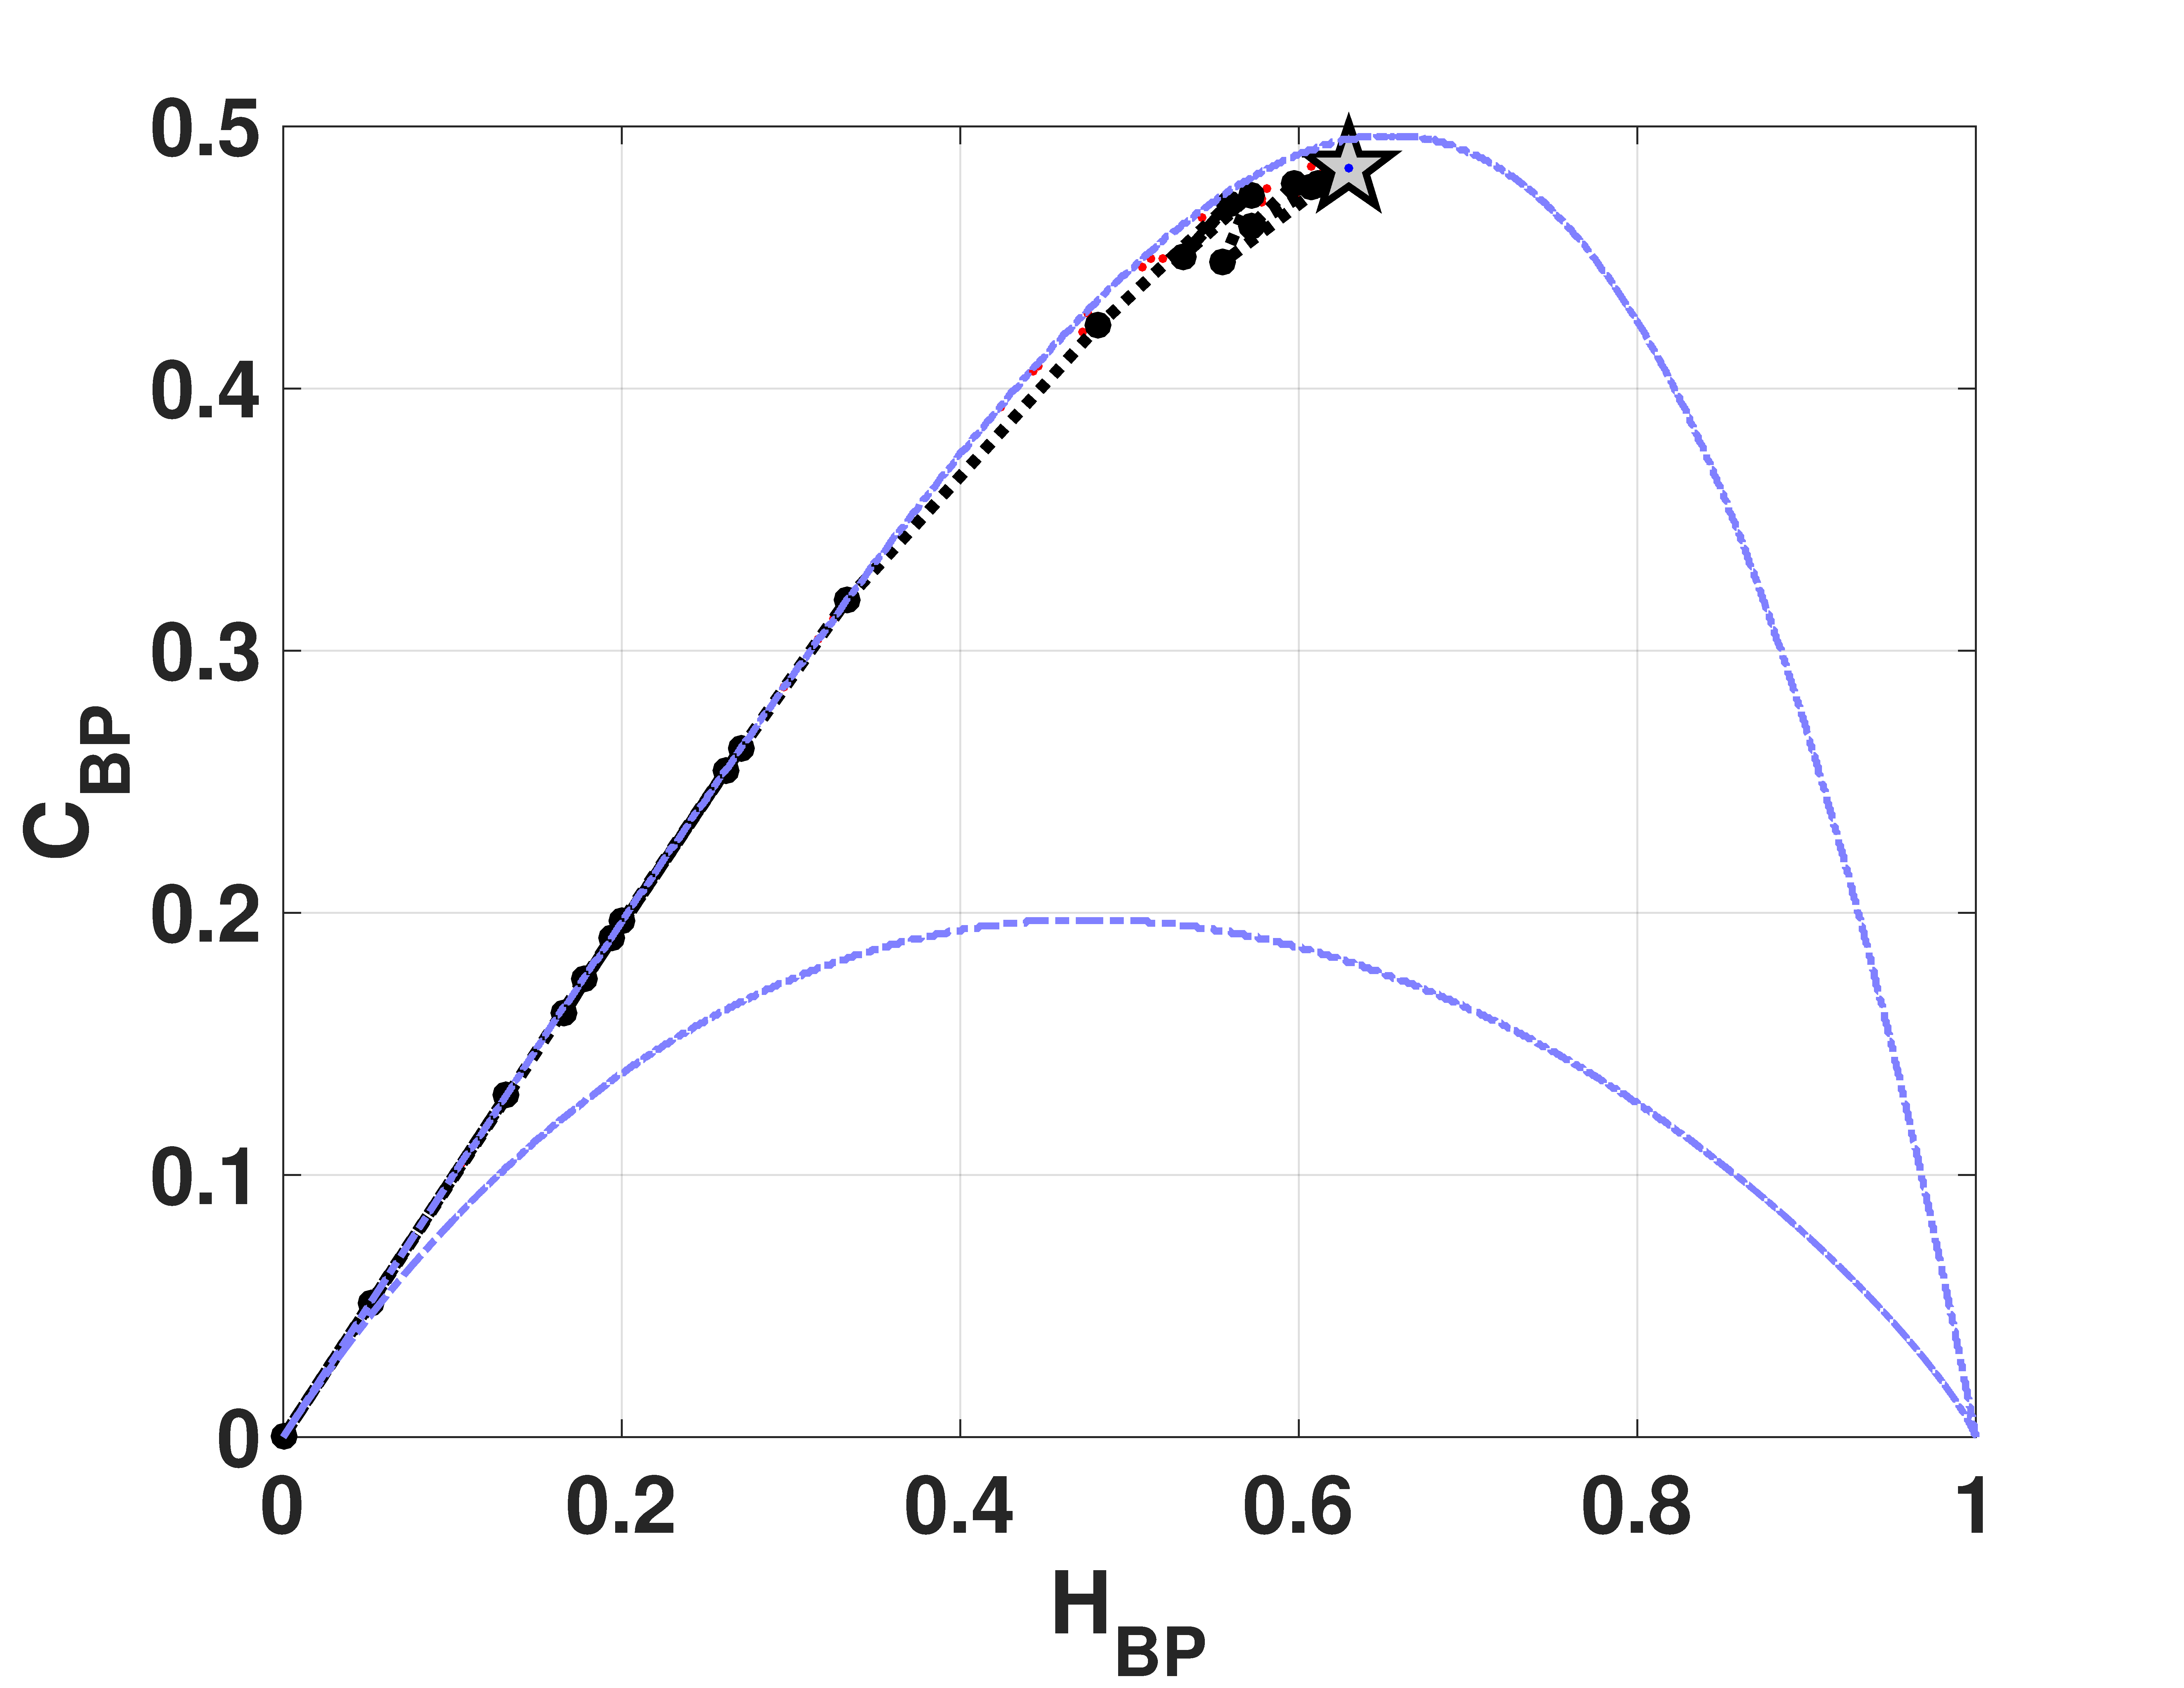
\includegraphics[width= .49\textwidth]{CbpHbp_Log}
	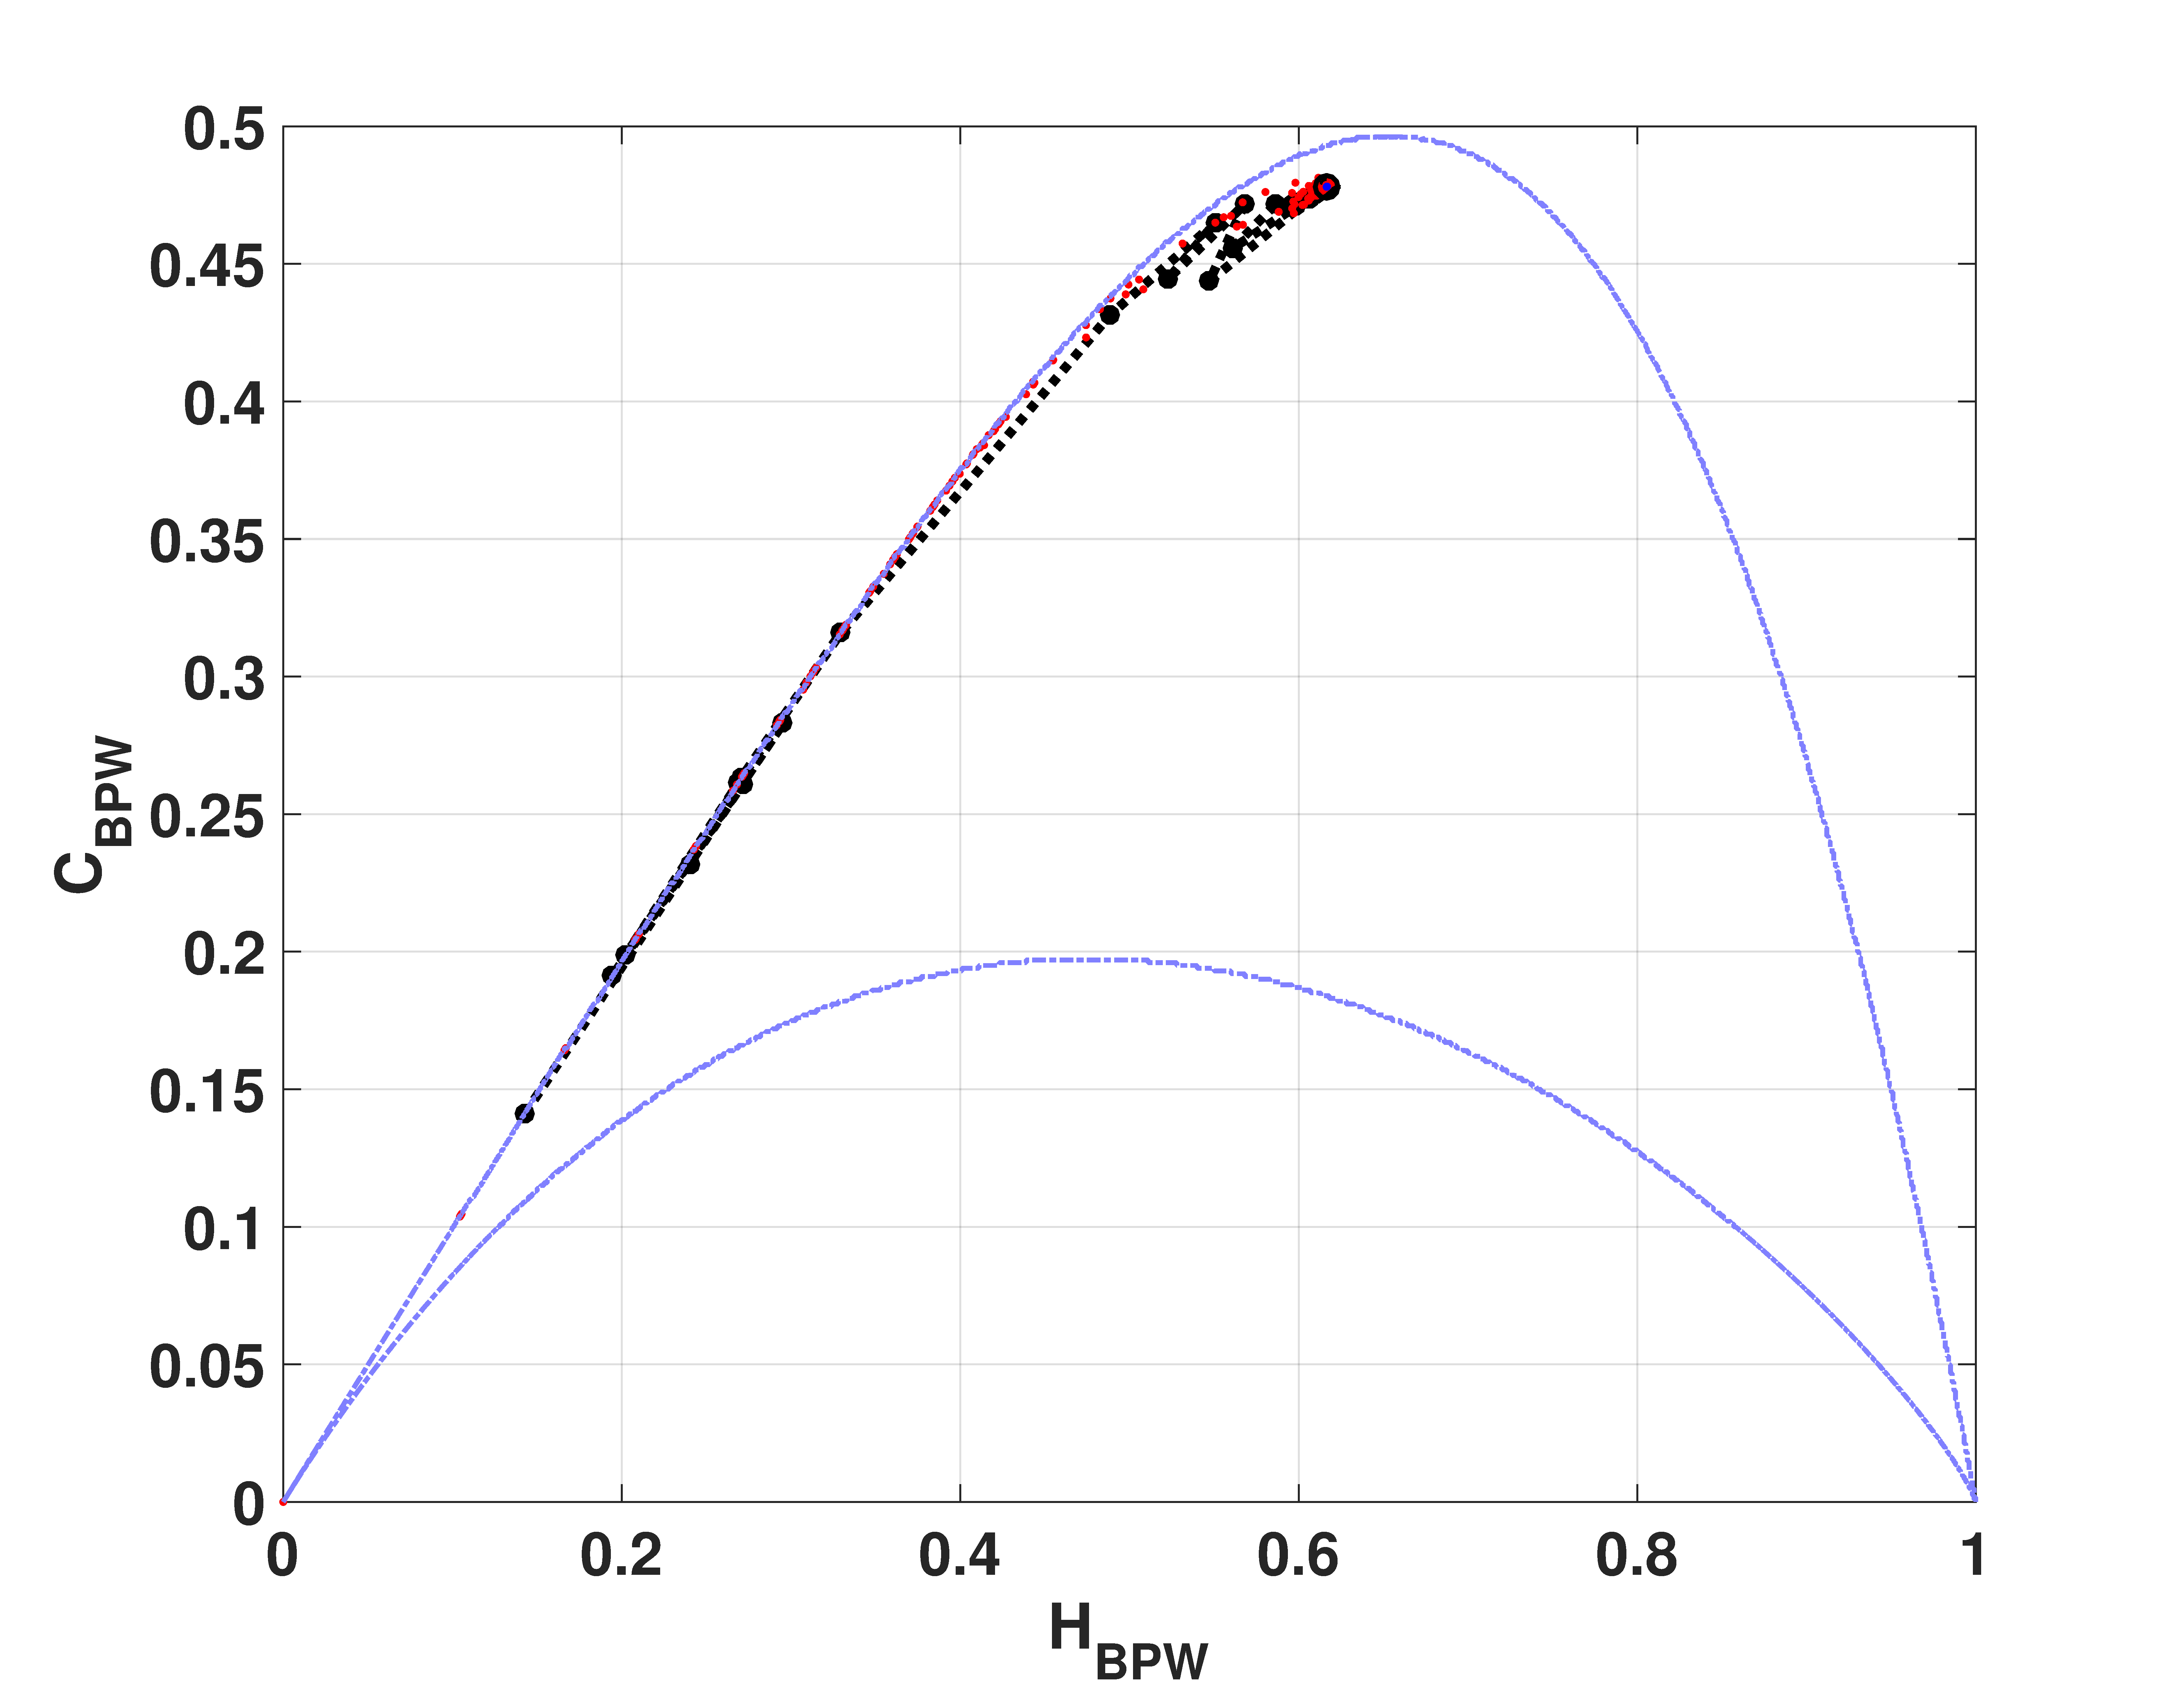
\includegraphics[width= .49\textwidth]{CbpwHbpw_Log}
	\caption{Evolution of statistical properties in entropy-complexity plane of LOG map: (a) $C_{BP}$ vs $H_{BP}$ (b) $C_{BPW}$ vs $H_{BPW}$.}
	\label{fig:LOG_HC}
\end{figure}


\subsubsection{TENT} \label{sssec:tent}

When this map is implemented in a computer using any numerical representation system (even floating-point!) truncation errors rapidly increase and make unstable fixed point in $x^*=0$ to become stable.
The sequences within the attractor domain of this fixed point will have a short transitory of length between $0$ and $B$ followed by an infinite number of $0$'s \cite{Jessa2002,Callegari}.
This issue is easily explained in \cite{Li2004}, the problem appears because all iterations have a left-shift operation that carries the $0$'s from the right side of the number to the most significant positions.

Figs. \ref{fig:Hval_Tent} to \ref{fig:MP_Tent} show the quantifiers for floating- and fixed-point numerical representations.
Quantifiers $H_{hist}$, $H_{BP}$ and $C_{BP}$ are equal to zero for all precisions, this reflects that the series quickly converge toward a fixed point for all sequences.
In the case of $H_{BPW}$ and $C_{BPW}$ quantifiers are different to non-null because BPW procedure discards the elements once they reach the fixed point.
The high dispersions in $H_{BPW}$, $C_{BPW}$ and MP are related to the short length of series transient.
These transients that converge to a fixed point have a maximum length of $B$ iterations for fixed-point arithmetic and $80$ for floating-point (long double precision).

\begin{figure}[htpb]
	\centering
	\begin{subfigure}[b]{0.49\textwidth}
		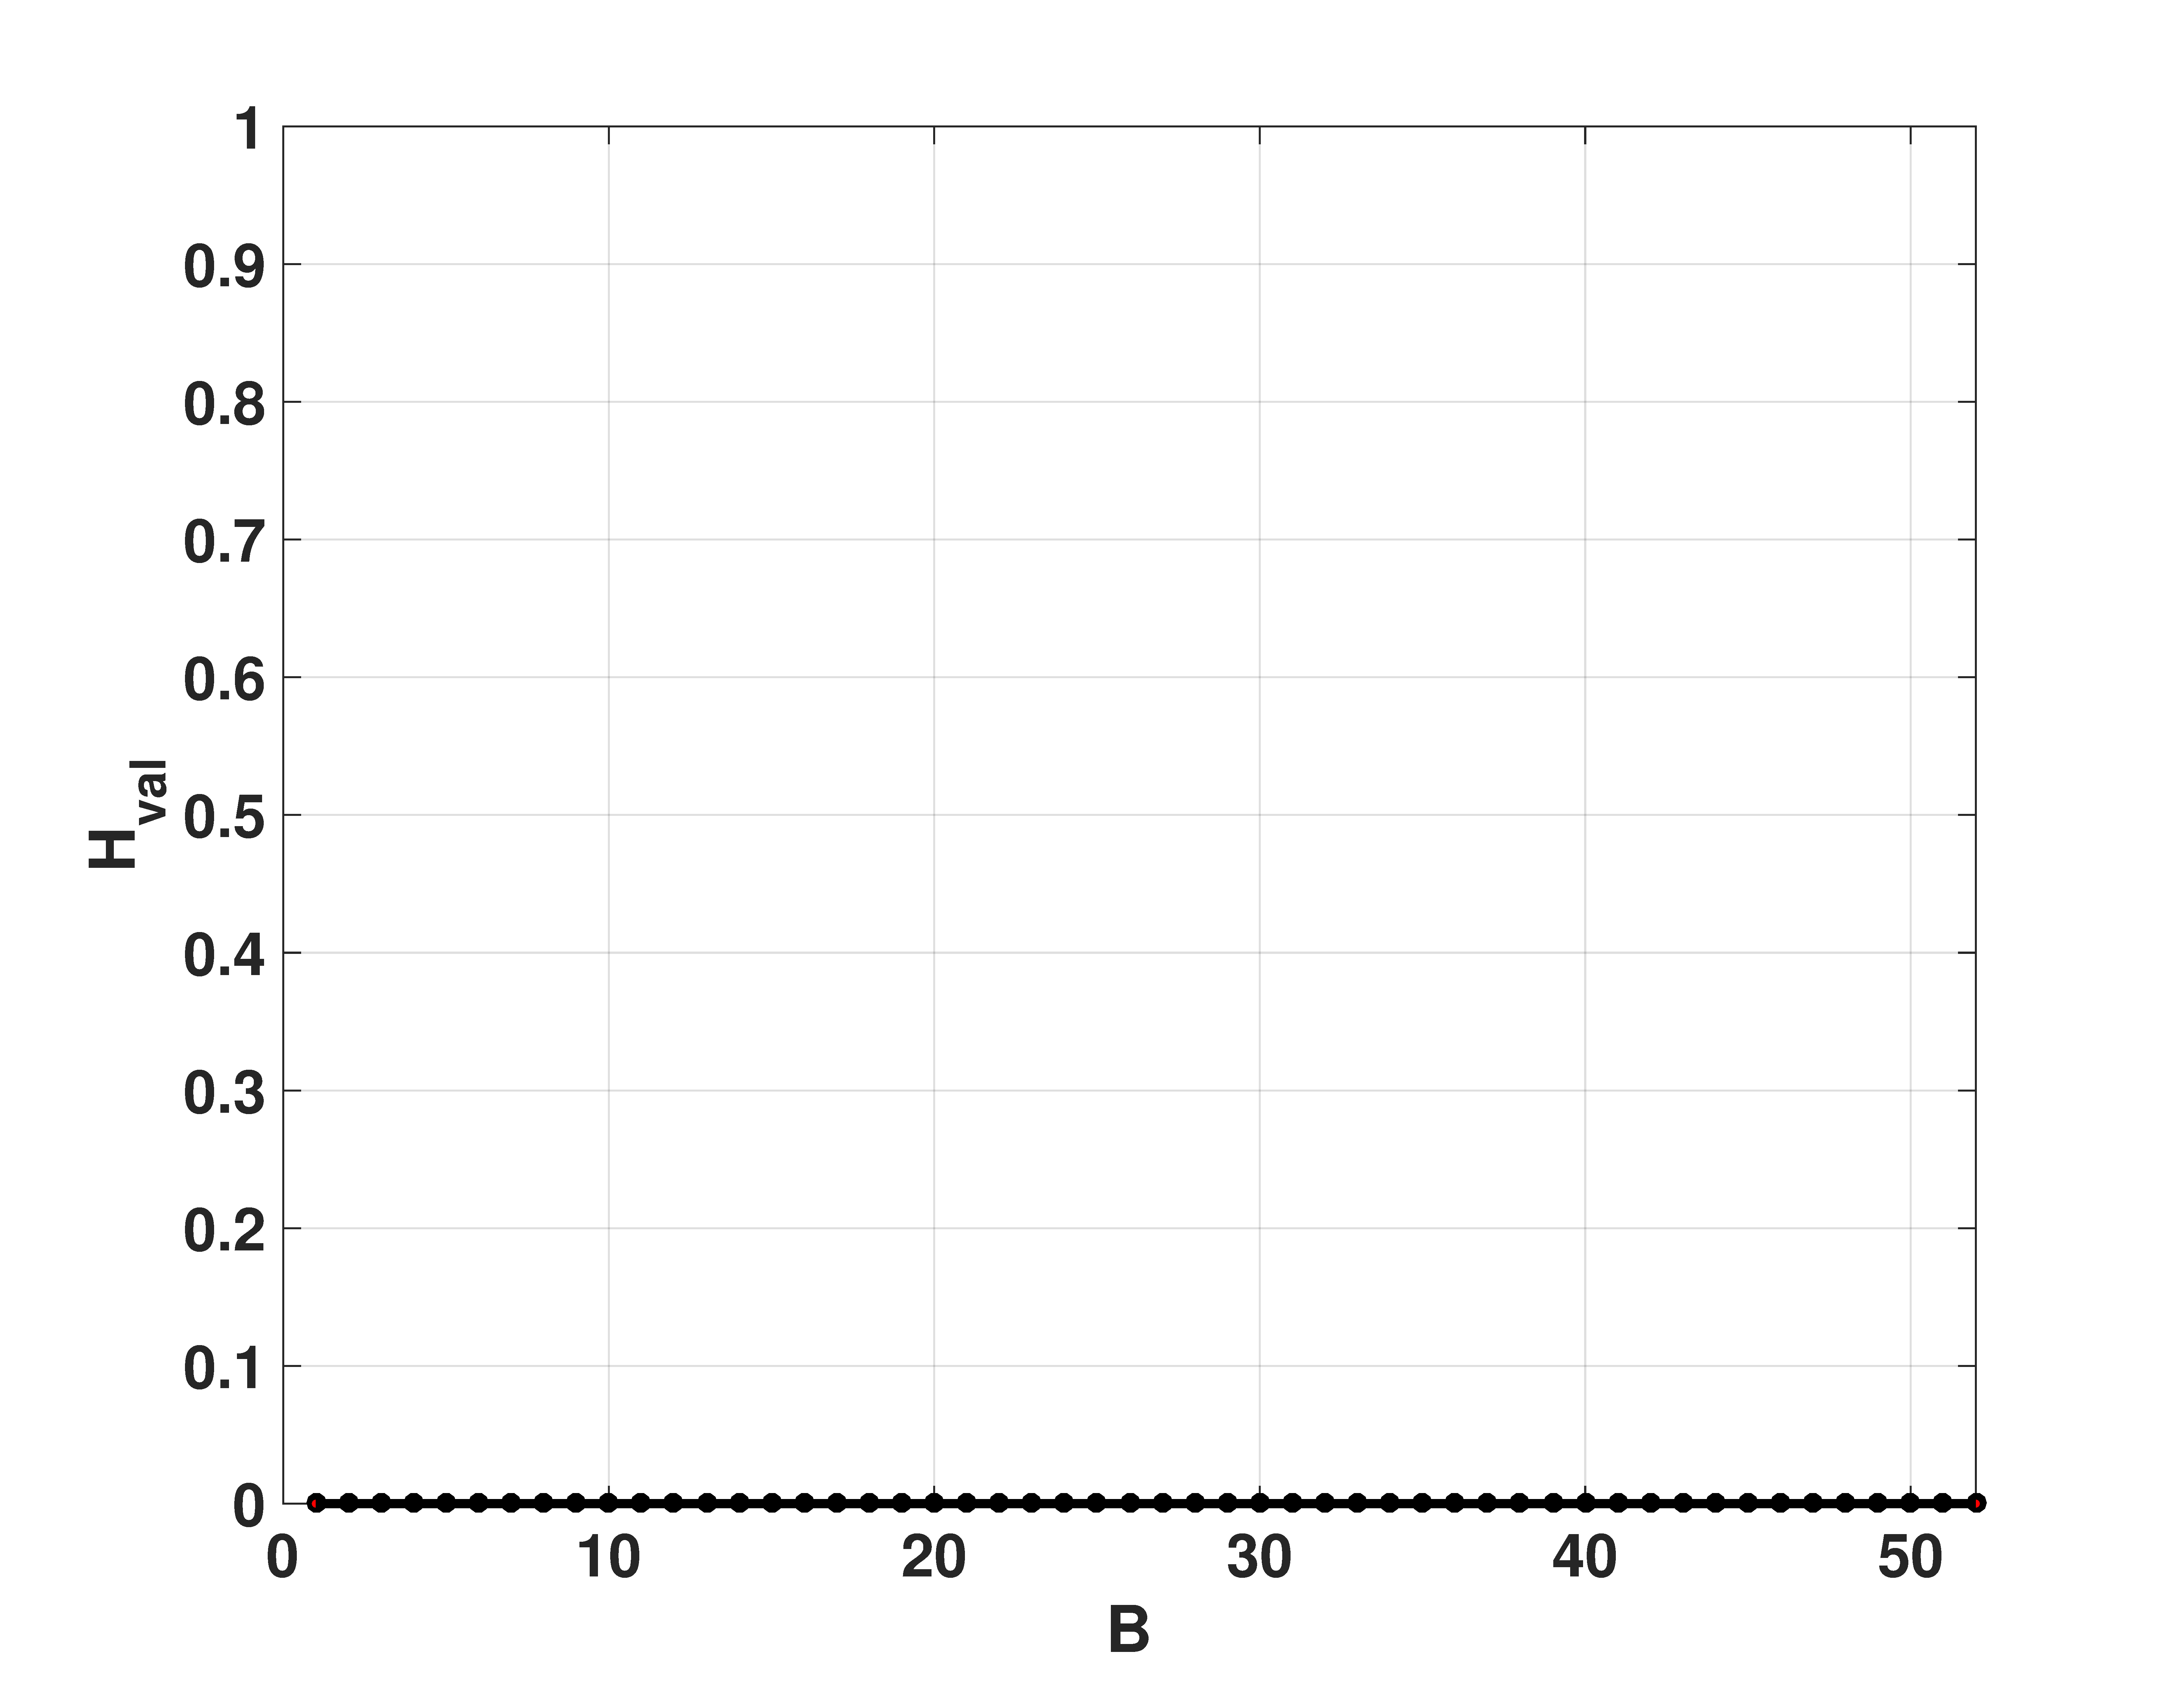
\includegraphics[width=\textwidth]{Hval_Tent}
		\caption{$H_{hist}$ vs. $B$}
		\label{fig:Hval_Tent}
	\end{subfigure}
	\begin{subfigure}[b]{0.49\textwidth}
		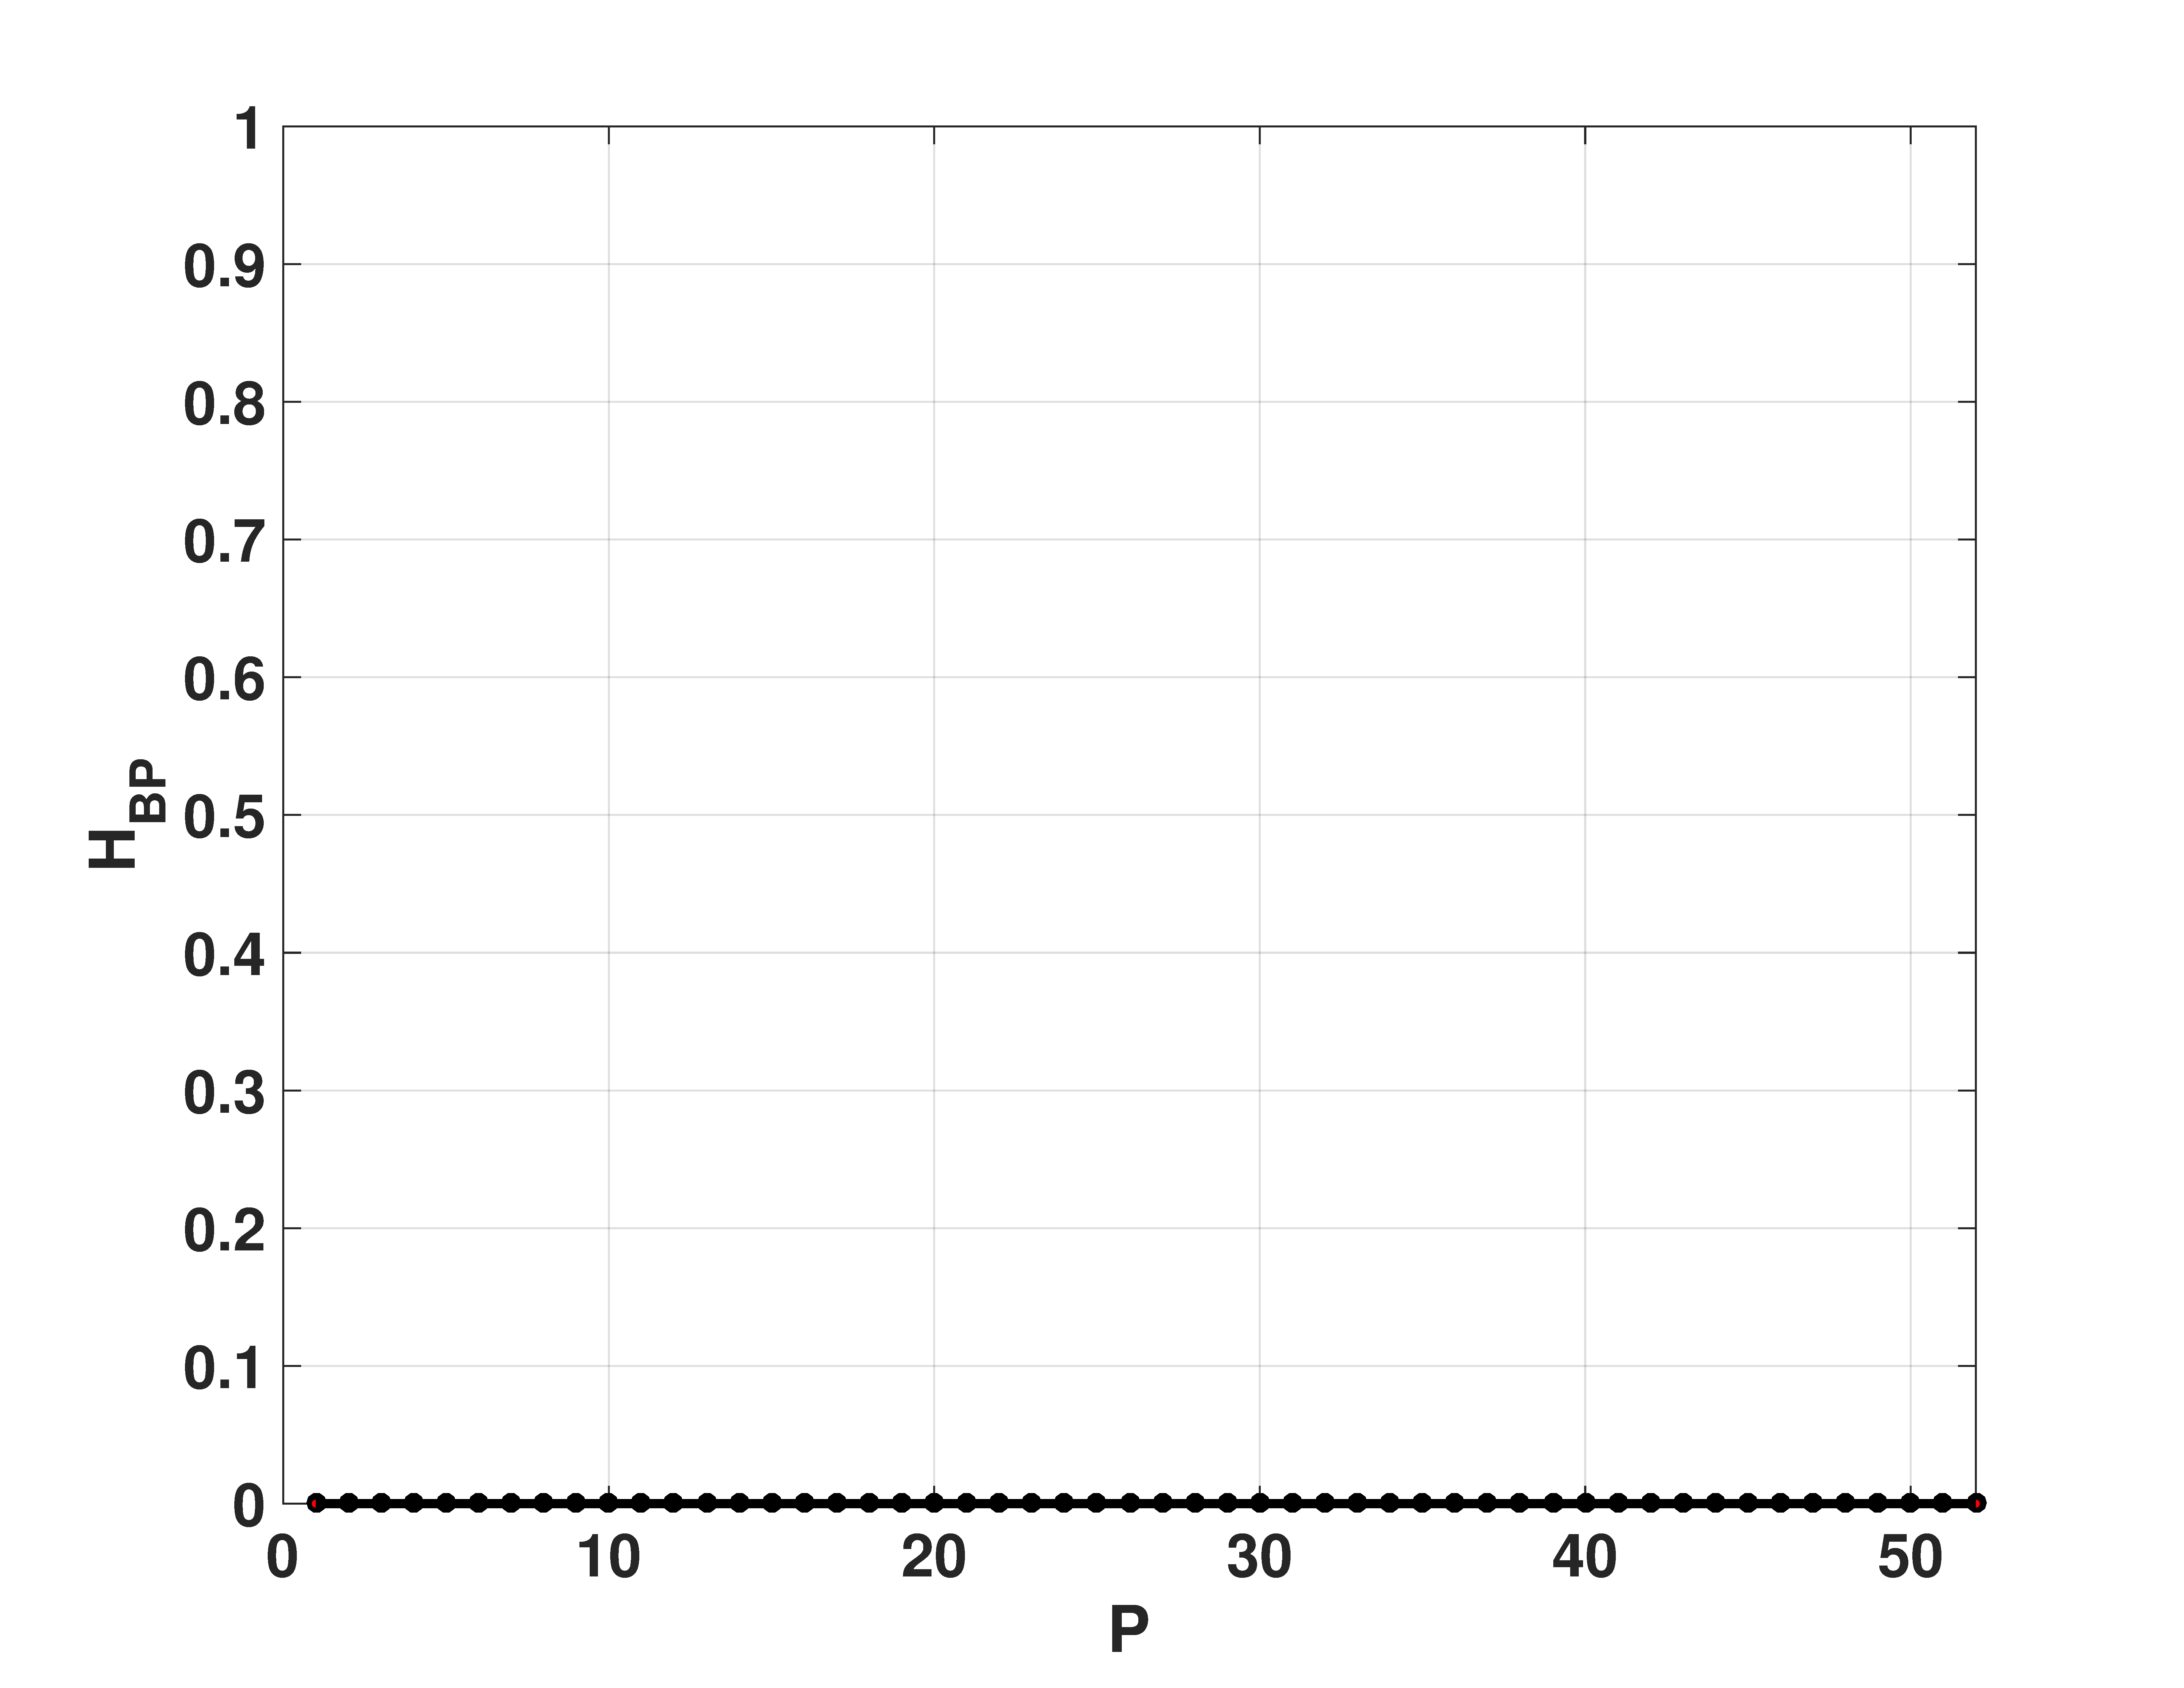
\includegraphics[width=\textwidth]{Hbp_Tent}
		\caption{$H_{BP}$ vs. $B$}
		\label{fig:Hbp_Tent}
	\end{subfigure}
	\begin{subfigure}[b]{0.49\textwidth}
		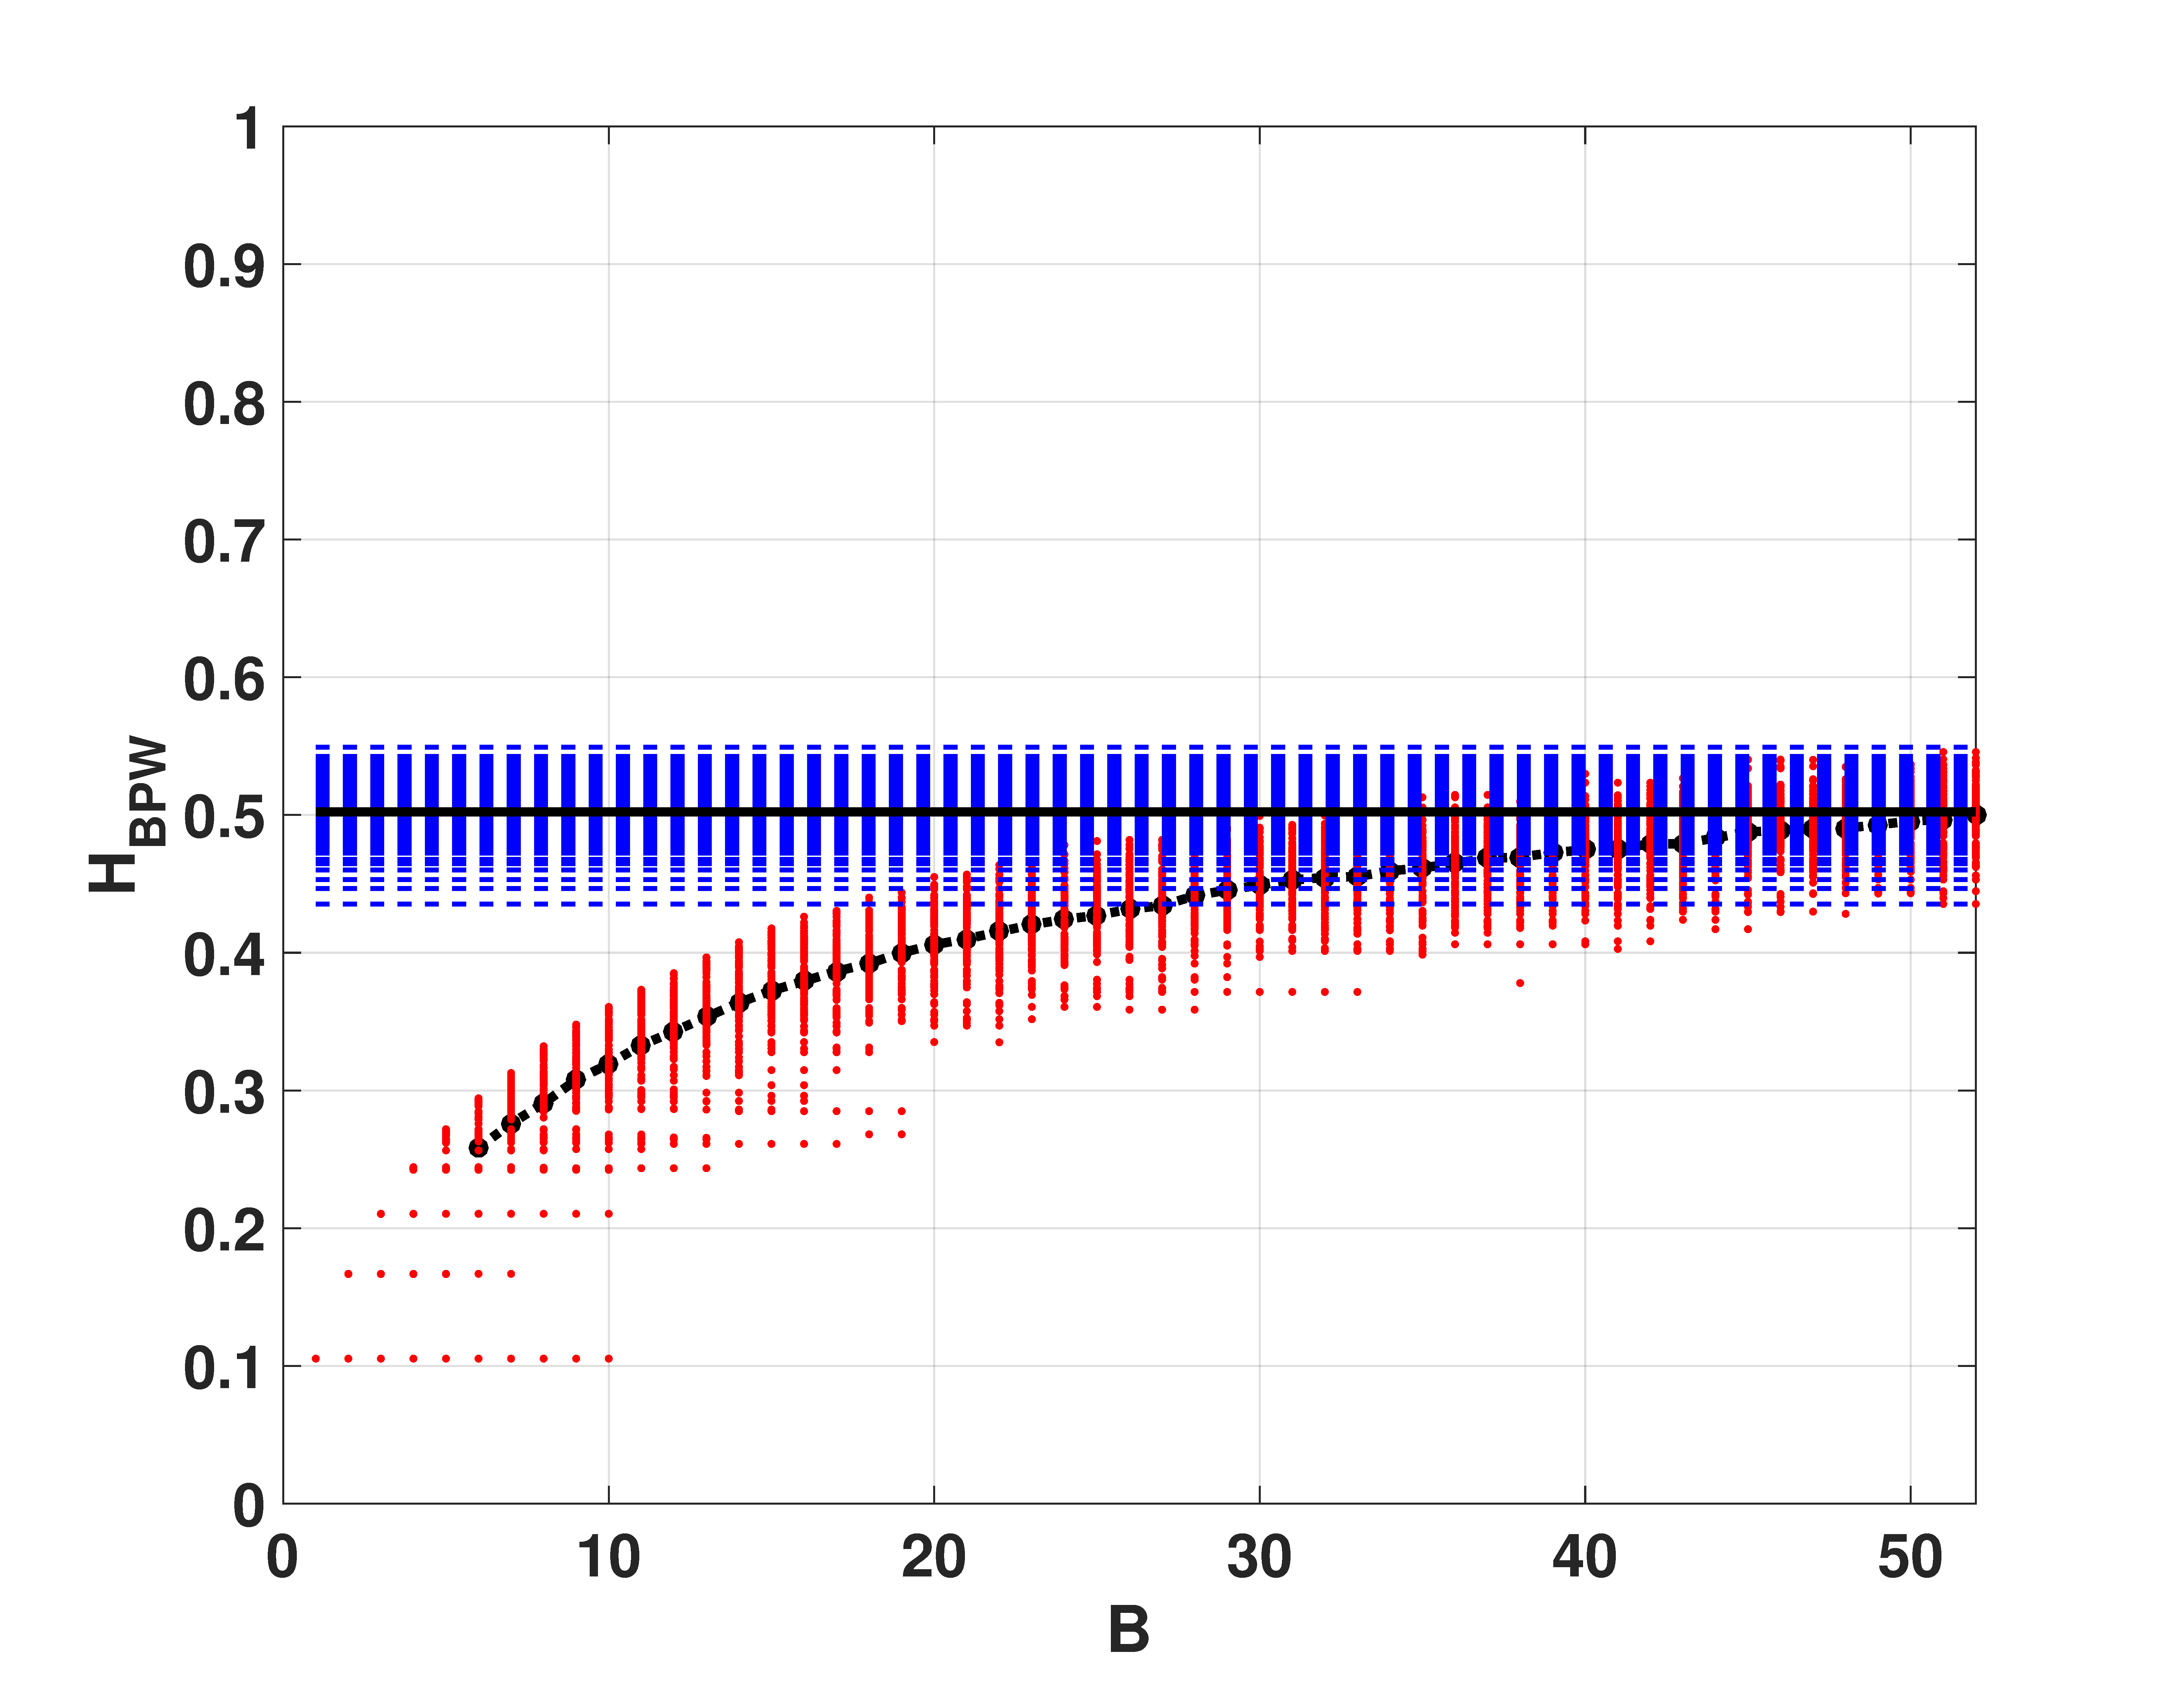
\includegraphics[width=\textwidth]{Hbpw_Tent}
		\caption{$H_{BPW}$ vs. $B$}
		\label{fig:Hbpw_Tent}
	\end{subfigure}
	\begin{subfigure}[b]{0.49\textwidth}
		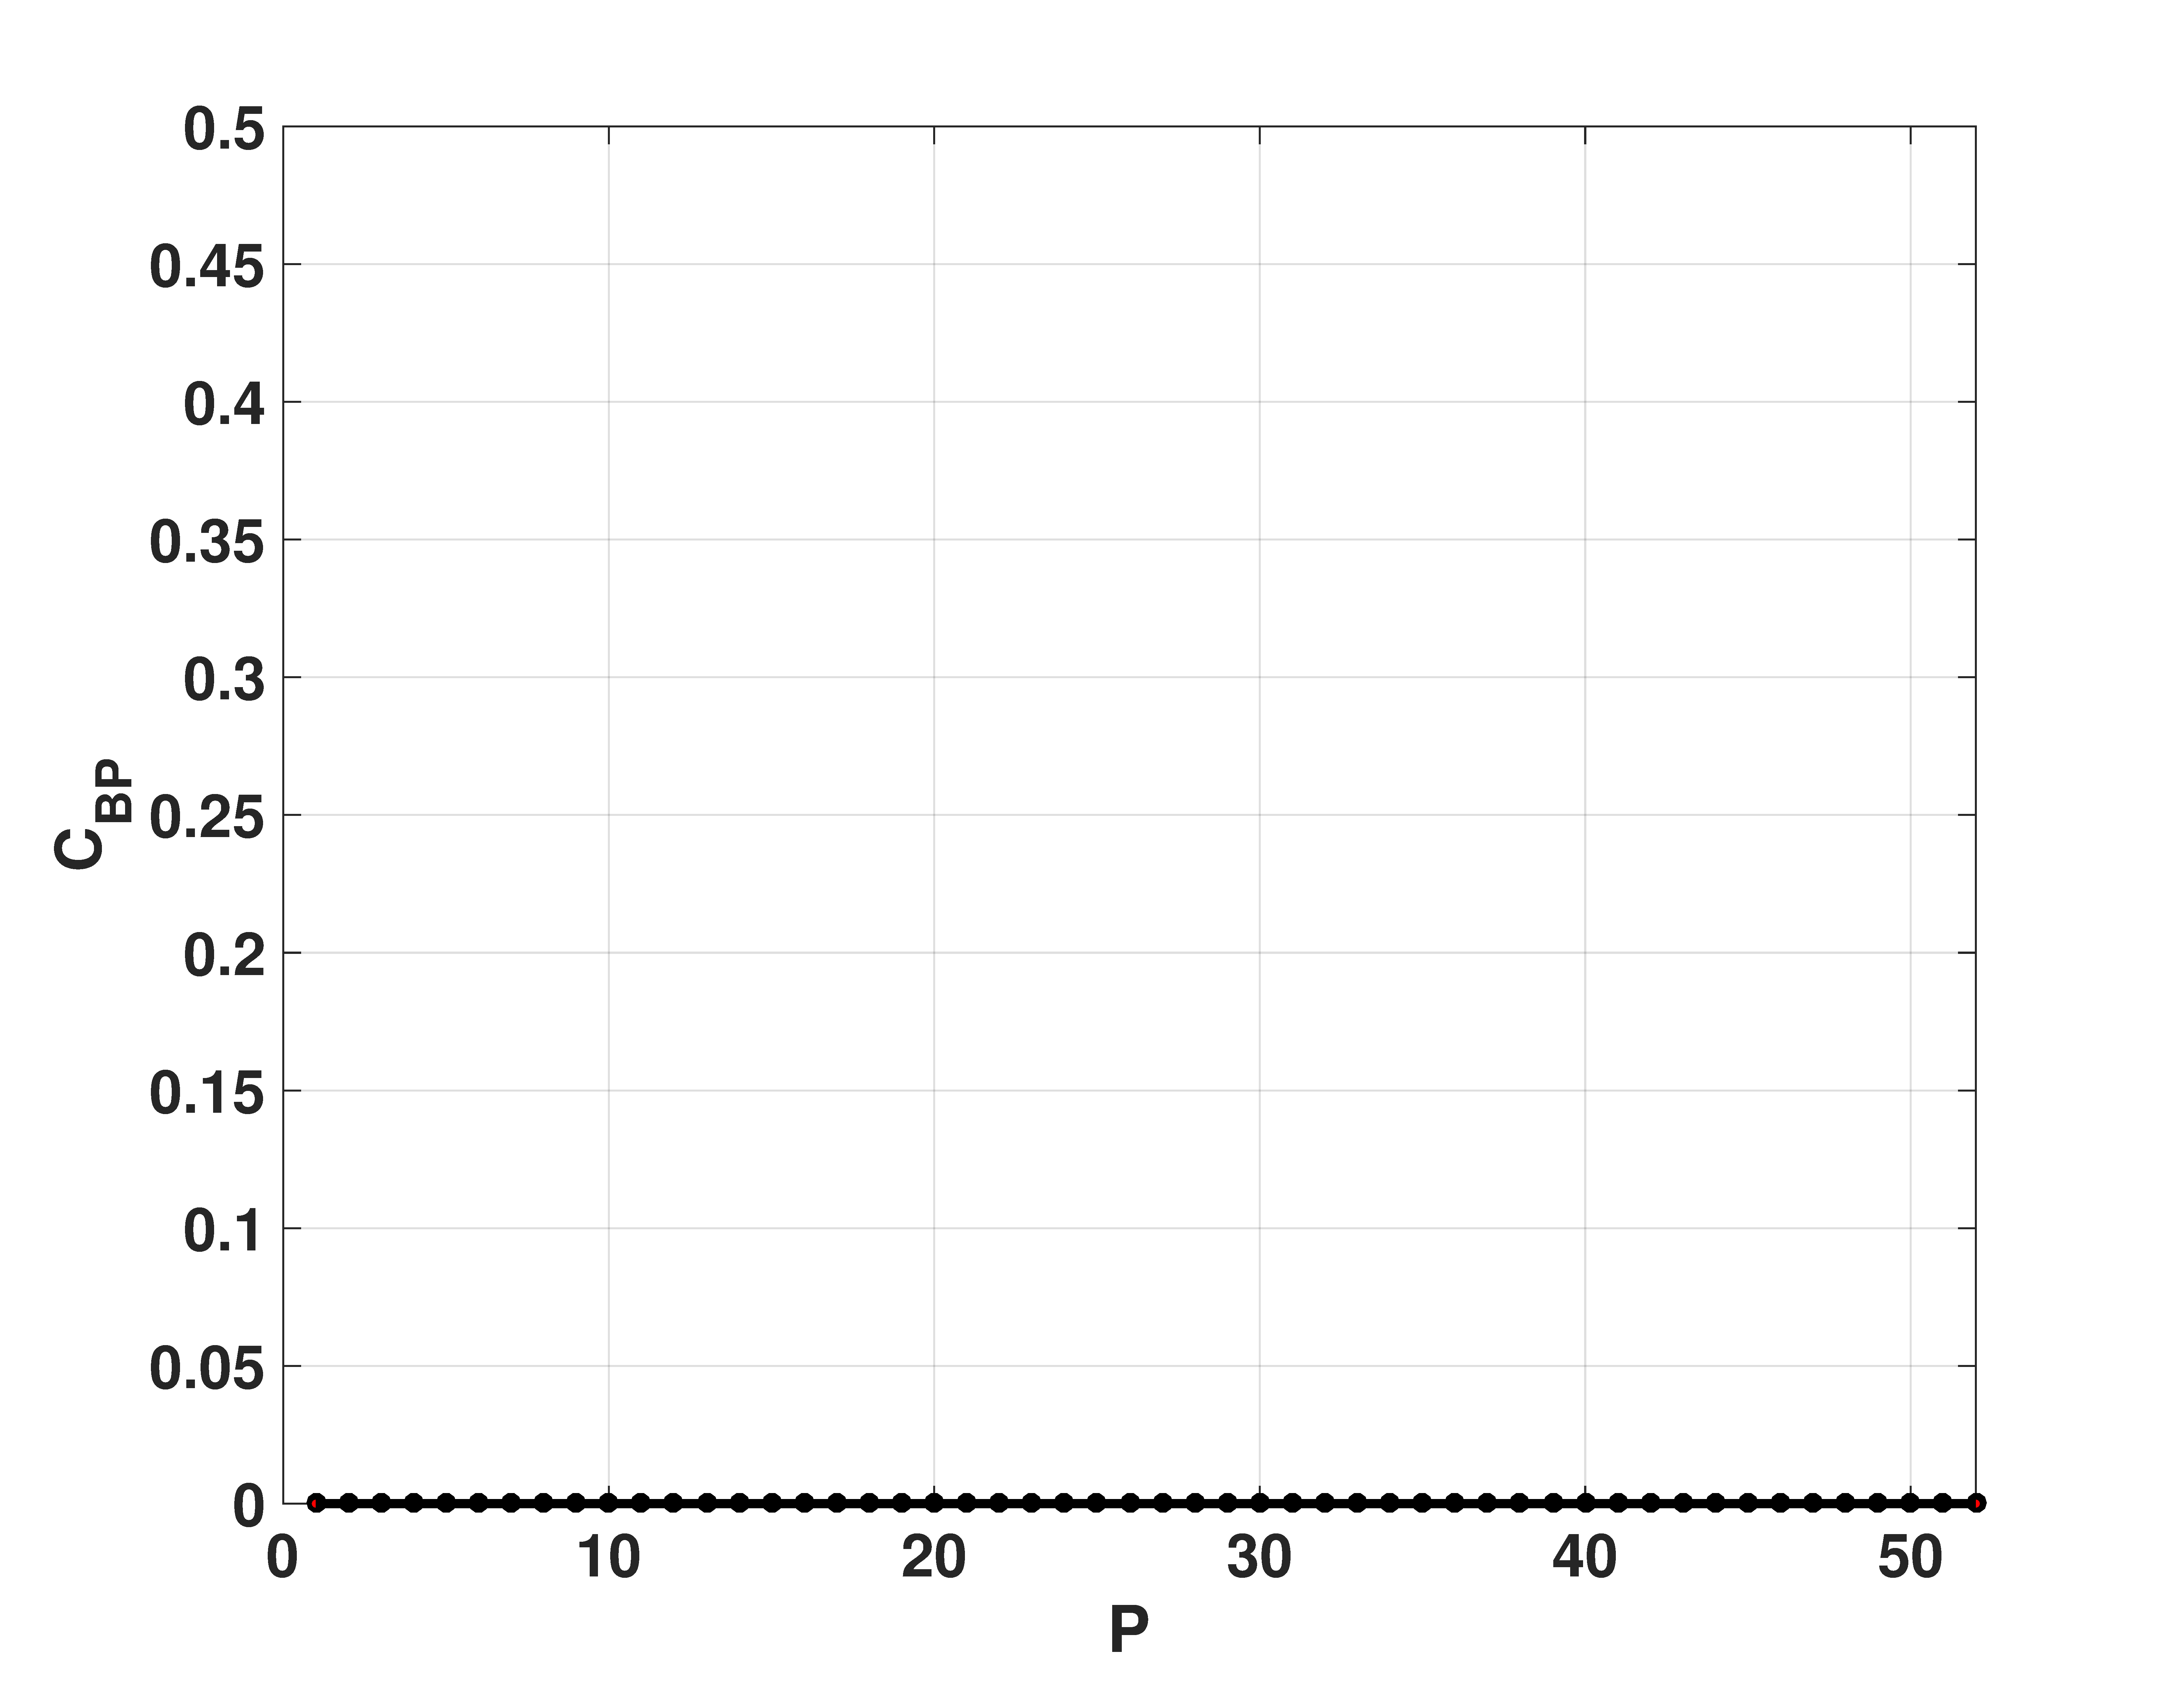
\includegraphics[width=\textwidth]{Cbp_Tent}
		\caption{$C_{BP}$ vs. $B$}
		\label{fig:Cbp_Tent}
	\end{subfigure}
	\begin{subfigure}[b]{0.49\textwidth}
		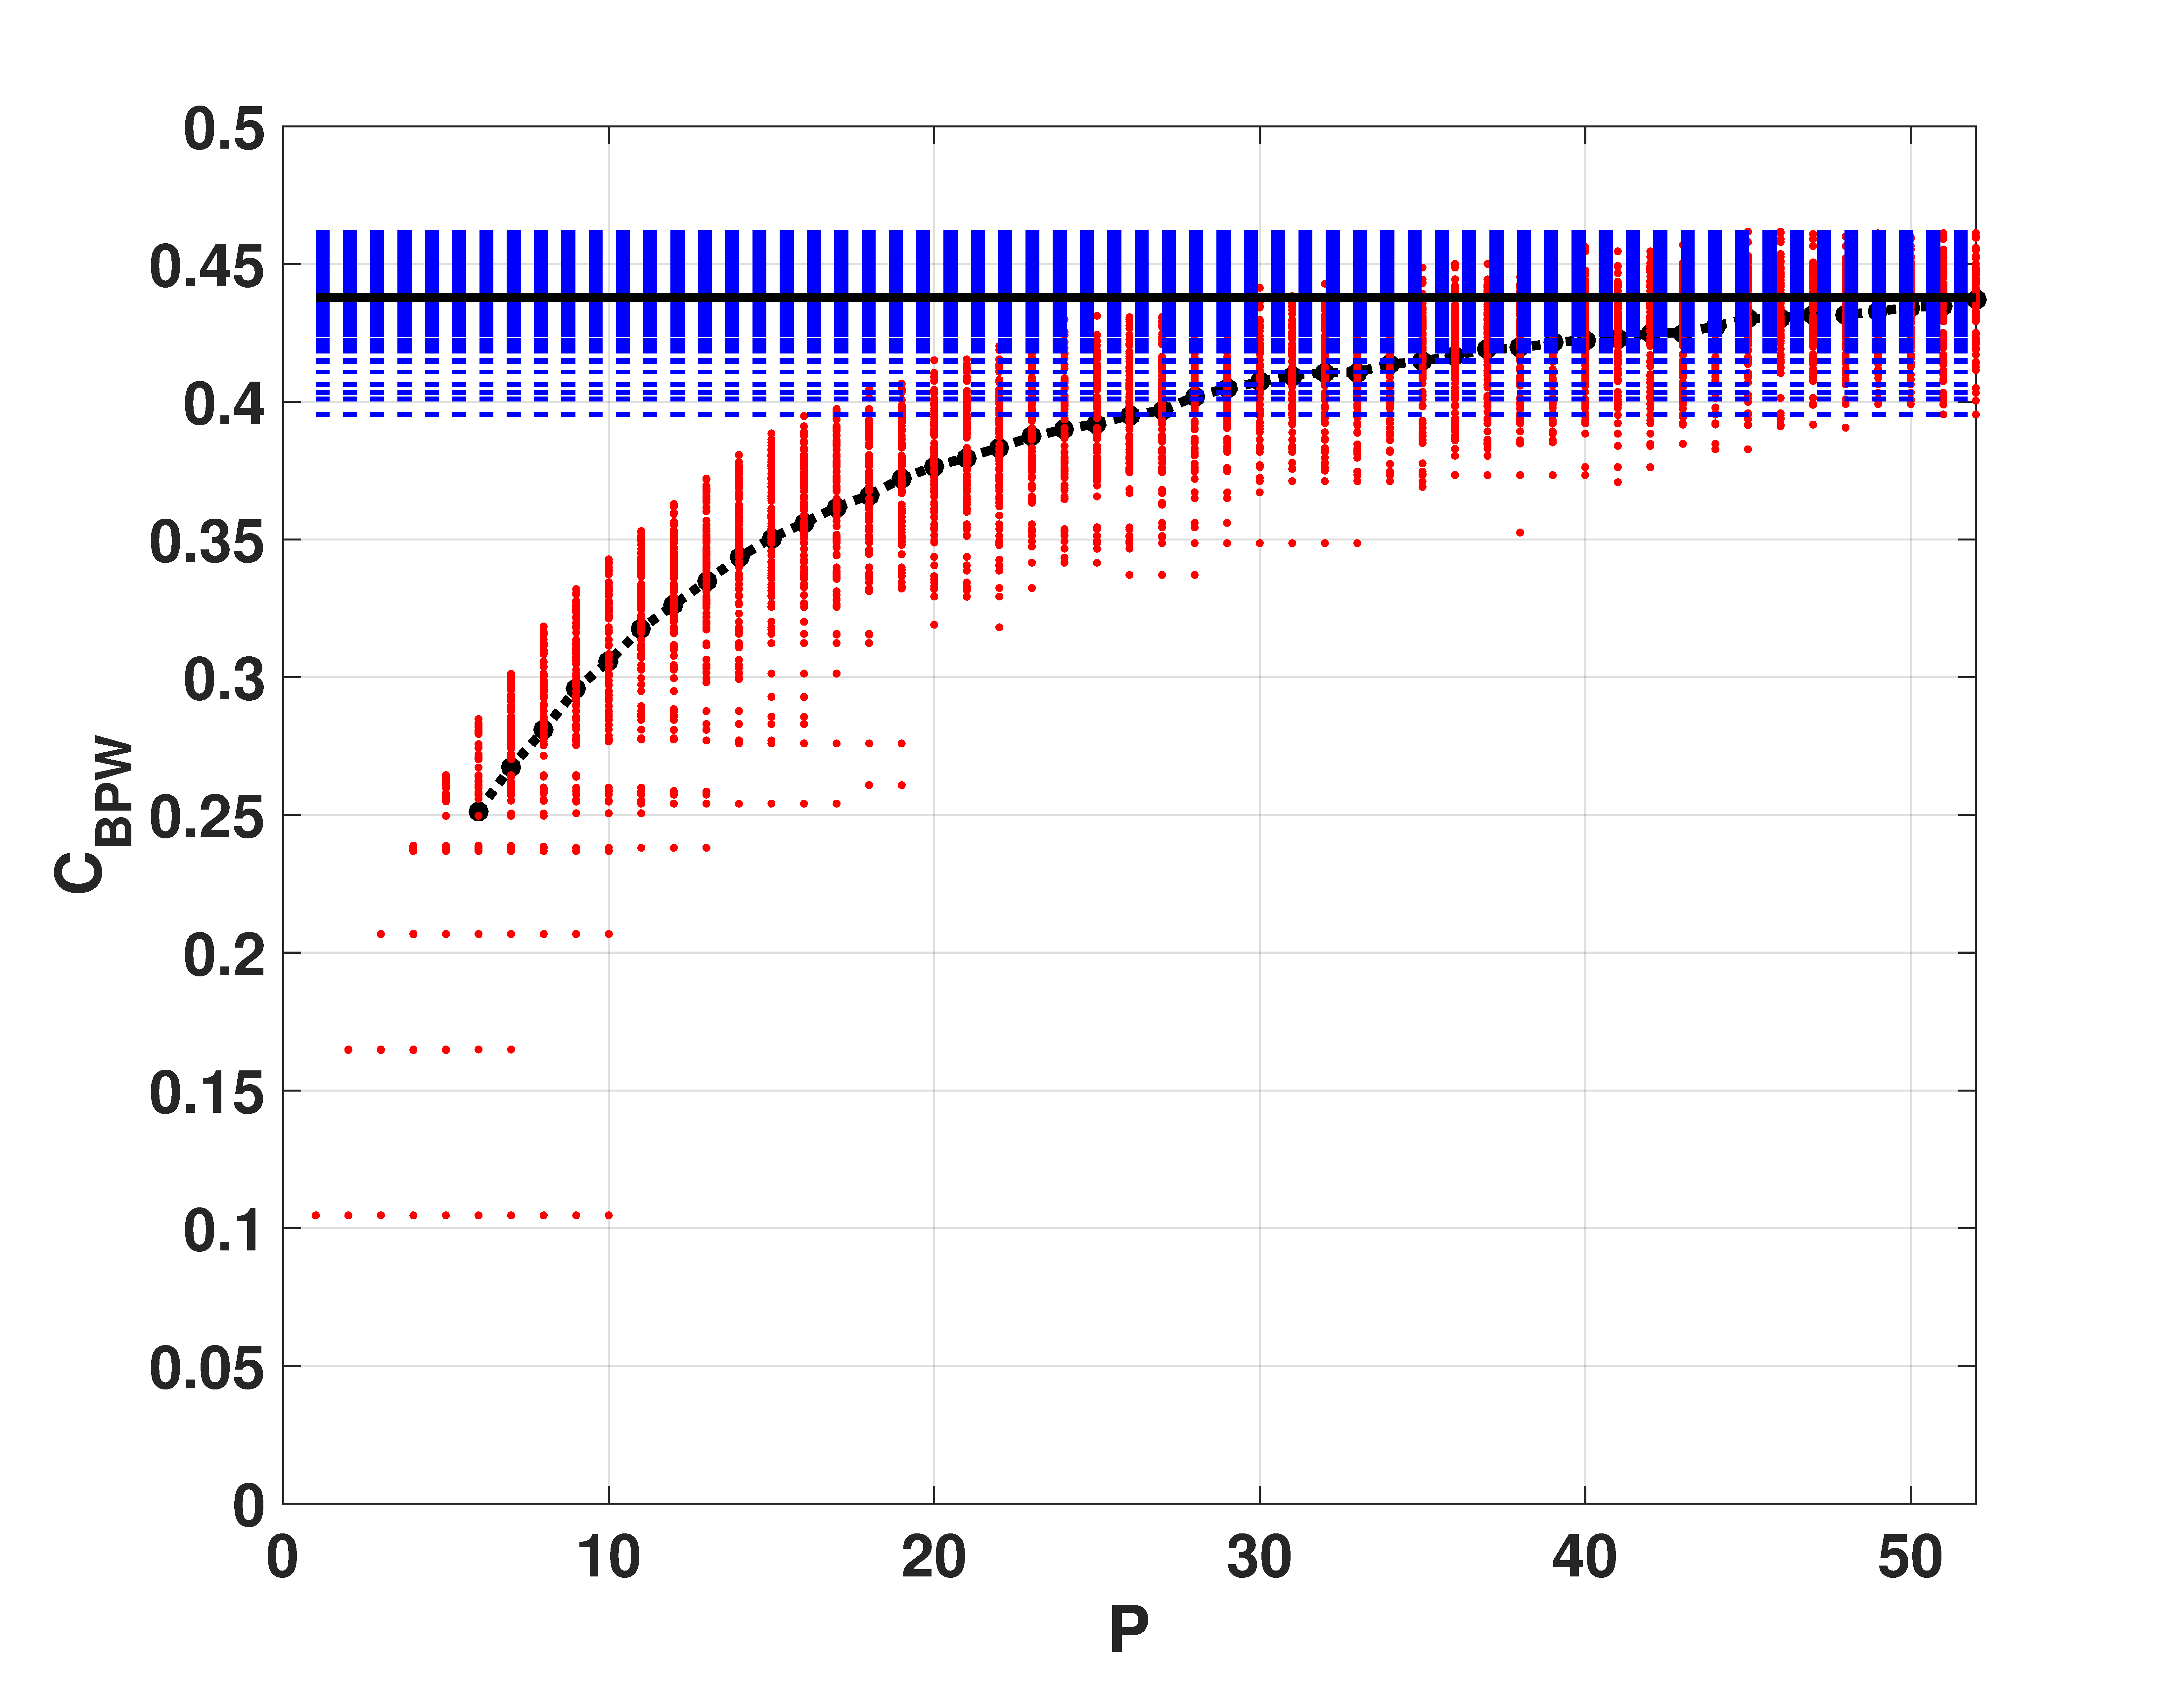
\includegraphics[width=\textwidth]{Cbpw_Tent}
		\caption{$C_{BPW}$ vs. $B$}
		\label{fig:Cbpw_Tent}
	\end{subfigure}
	\begin{subfigure}[b]{0.49\textwidth}
		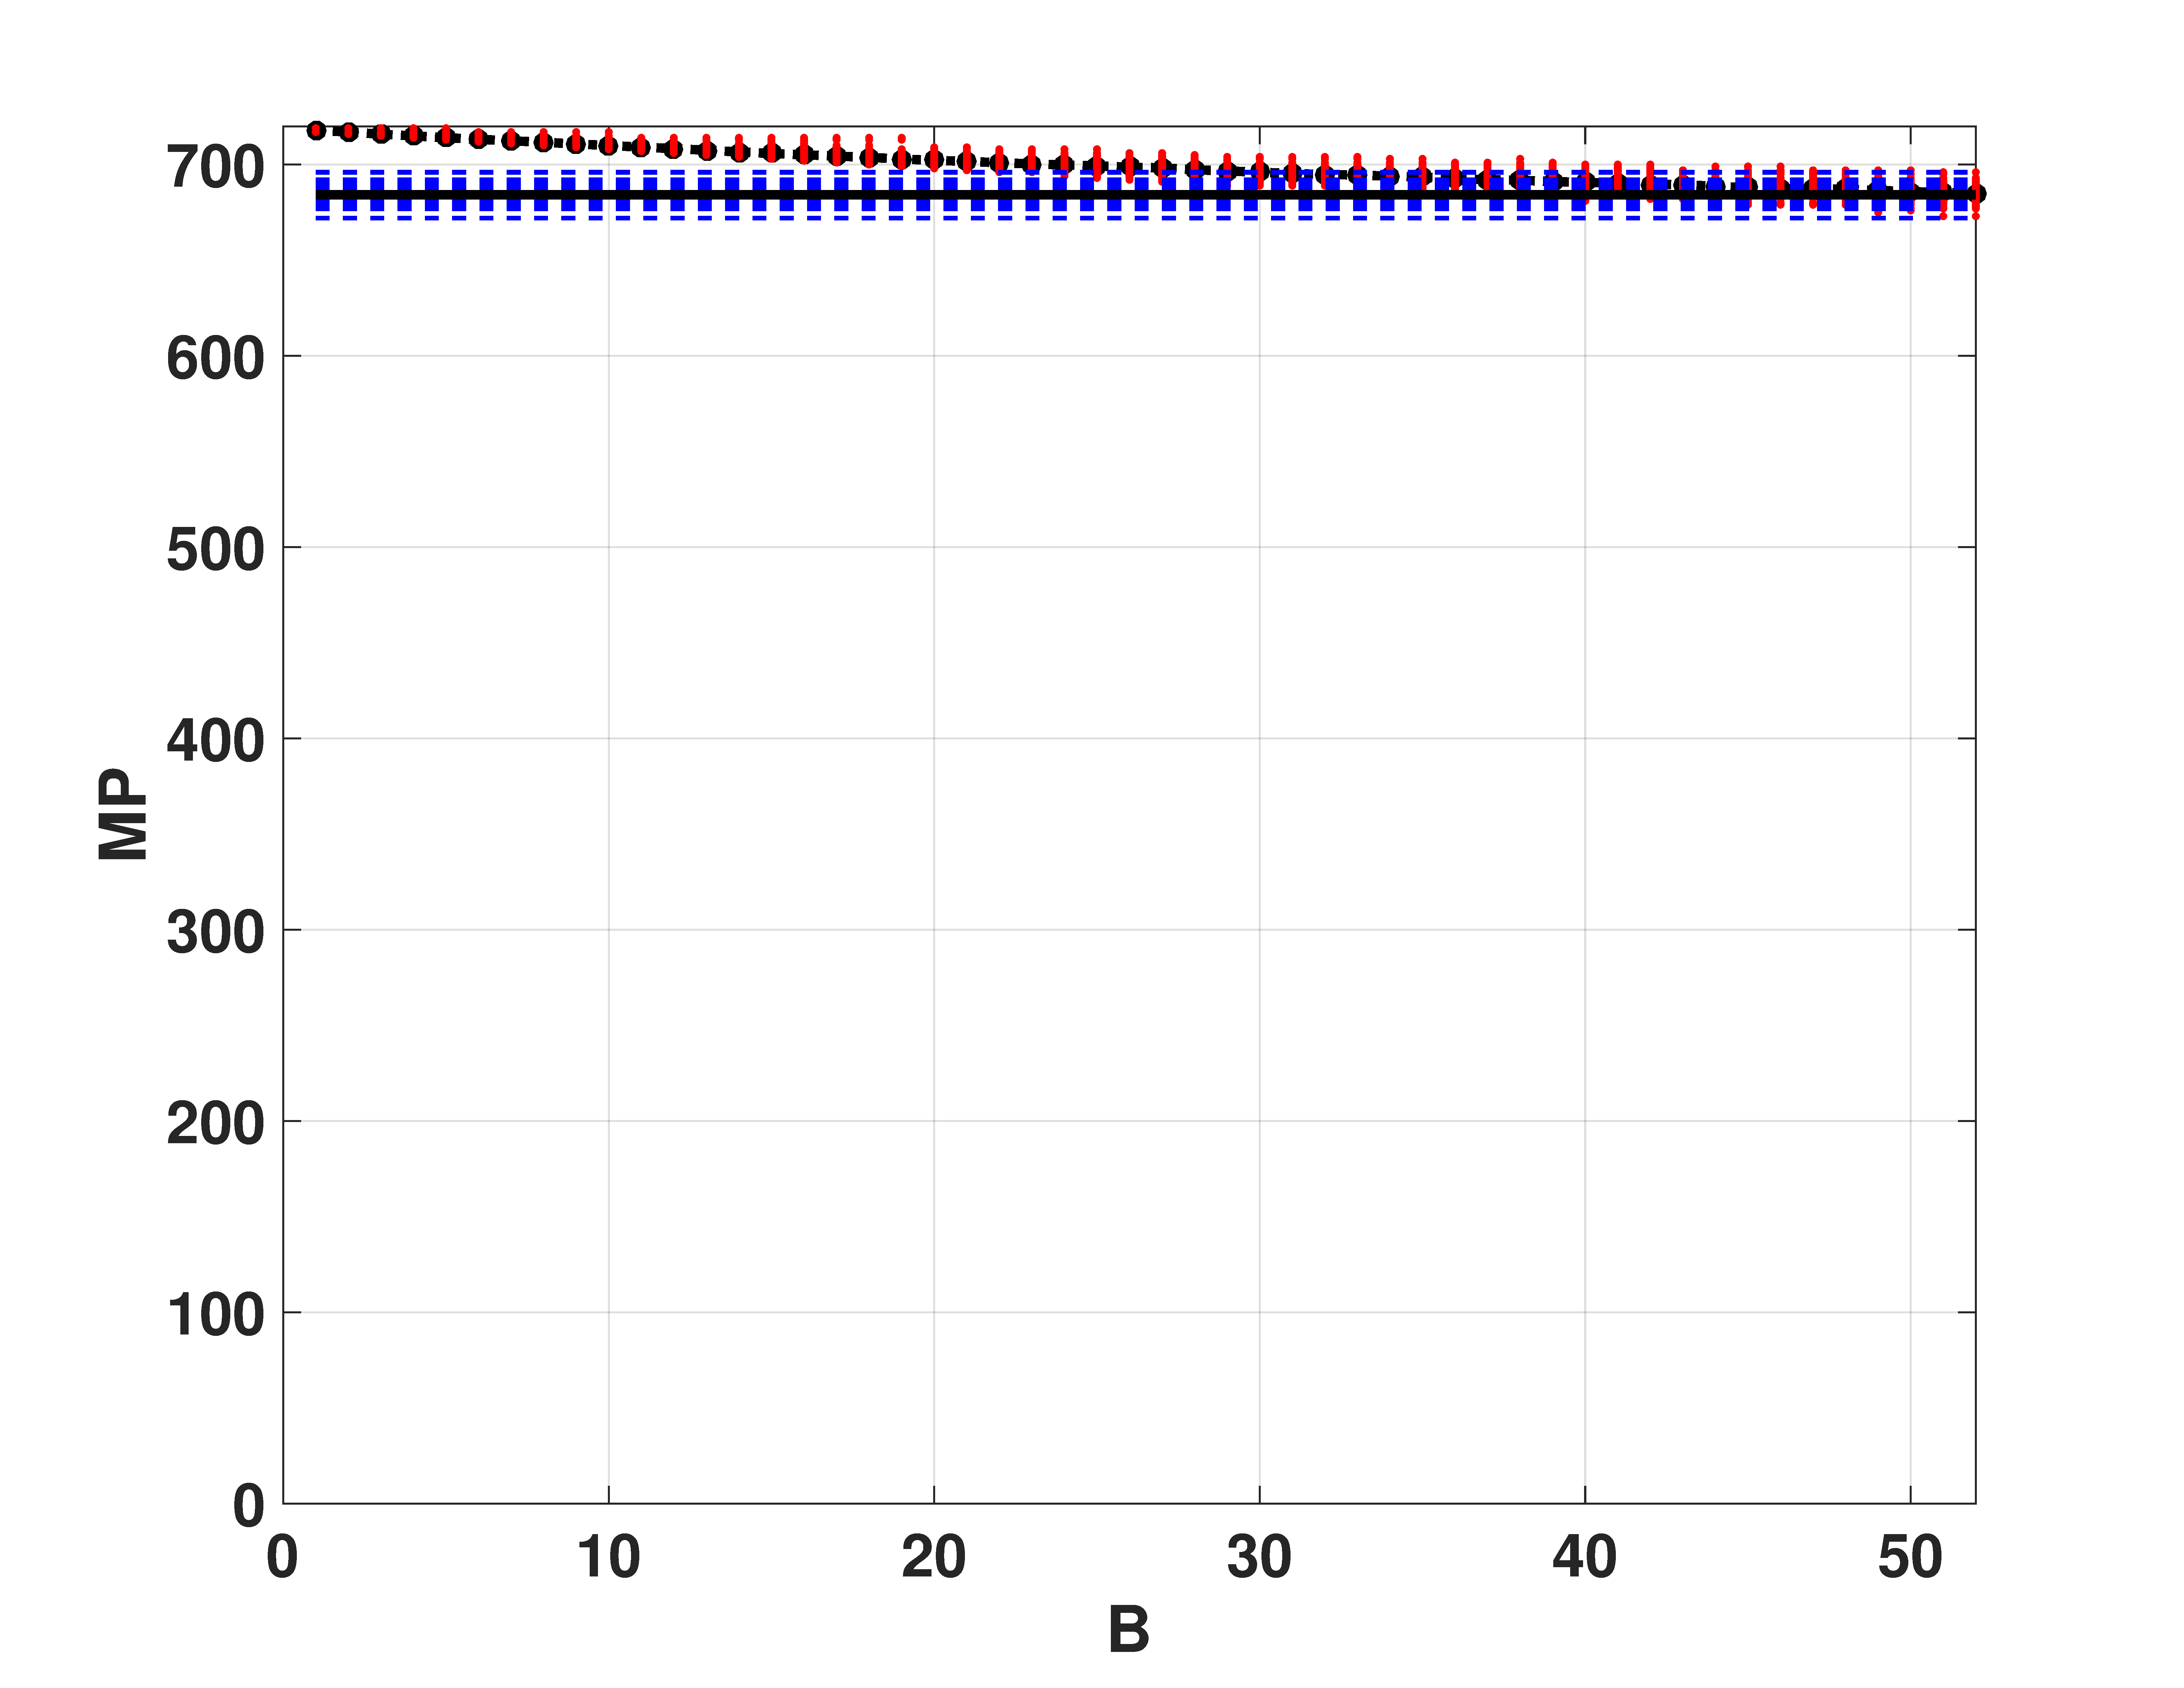
\includegraphics[width=\textwidth]{MP_Tent}
		\caption{MP vs. $B$}
		\label{fig:MP_Tent}
	\end{subfigure}
	\caption{Statistical properties of TENT map}
	\label{fig:TENT_QuantiB}
\end{figure}

Summarizing, in spite of using a high number of bits (with any 2-based numerical representation) to represent the digitalized TENT map it always loses the chaotic behaviour.
 

\subsection{Quantifiers of combined Maps}\label{subsec:SecSwitch}
Here we report our results for the three combinations of the simple maps, SWITCH, EVEN and ODD.

\subsubsection{Sequential switching between Tent and Logistic maps (SWITCH)} \label{sssec:switch}

SWITCH map is expressed as:

\begin{equation}
\begin{cases}
	x_{n+1}=
	\begin{cases}
		2x_n, & \mbox{if } 0\leq x_n\leq 1/2 \\
		2(1-x_n ), & \mbox{if } 1/2<x_n\leq 1
	\end{cases} \\
	x_{n+2}=4x_{n+1}(1-x_{n+1})
\end{cases}\label{eq:SWITCH}
\end{equation}
with $x_n\in\mathcal{R}$ and $n$ an even number.

Results with sequential switching are shown in Figs. \ref{fig:SWITCH_QuantiB} (a) to (f).
The entropy value calculated in floating point is $H_{val}=0.9722$, this value is slightly higher than the one obtained for the LOG map. 
For fixed point arithmetic this value is reached in $B=24$, but it stabilizes from $B=28$.
Regarding the ordering patterns the number of MP decreases to $586$, this value lower than the one obtained for LOG map.
It means the entropy $H_{BP}$ may increase up to $ln(134)/ln(720)\simeq 0.74$.
$BP$ and $BPW$ quantifiers reach their maximum of $H_{BP}=0.6546$ and $H_{BPW}=0.6313$ at $B=16$, but they stabilize from $B=24$.
Complexities are lower than for LOG, $C_{BP}=0.4580$ and $C_{BPW}=0.4578$, these values are reached for $B \geq 15$ but they are stable from $B \geq 23$.
Compared with LOG, statistical properties are better with less amount of bits, for $B \geq 24$ this map reaches optimal characteristics in the sense of random source.

\textcolor{red}{ESTO NO SE SI VA A IR EN LONG DOUBLE}
We can see some points with anomalies from $B \geq 49$ due to the same problem of LOG map, an multiplication needs double of precision to be done.
Furthermore, we encountred one initial condition in fixed point with an anomalous behaviour.

\begin{figure}
	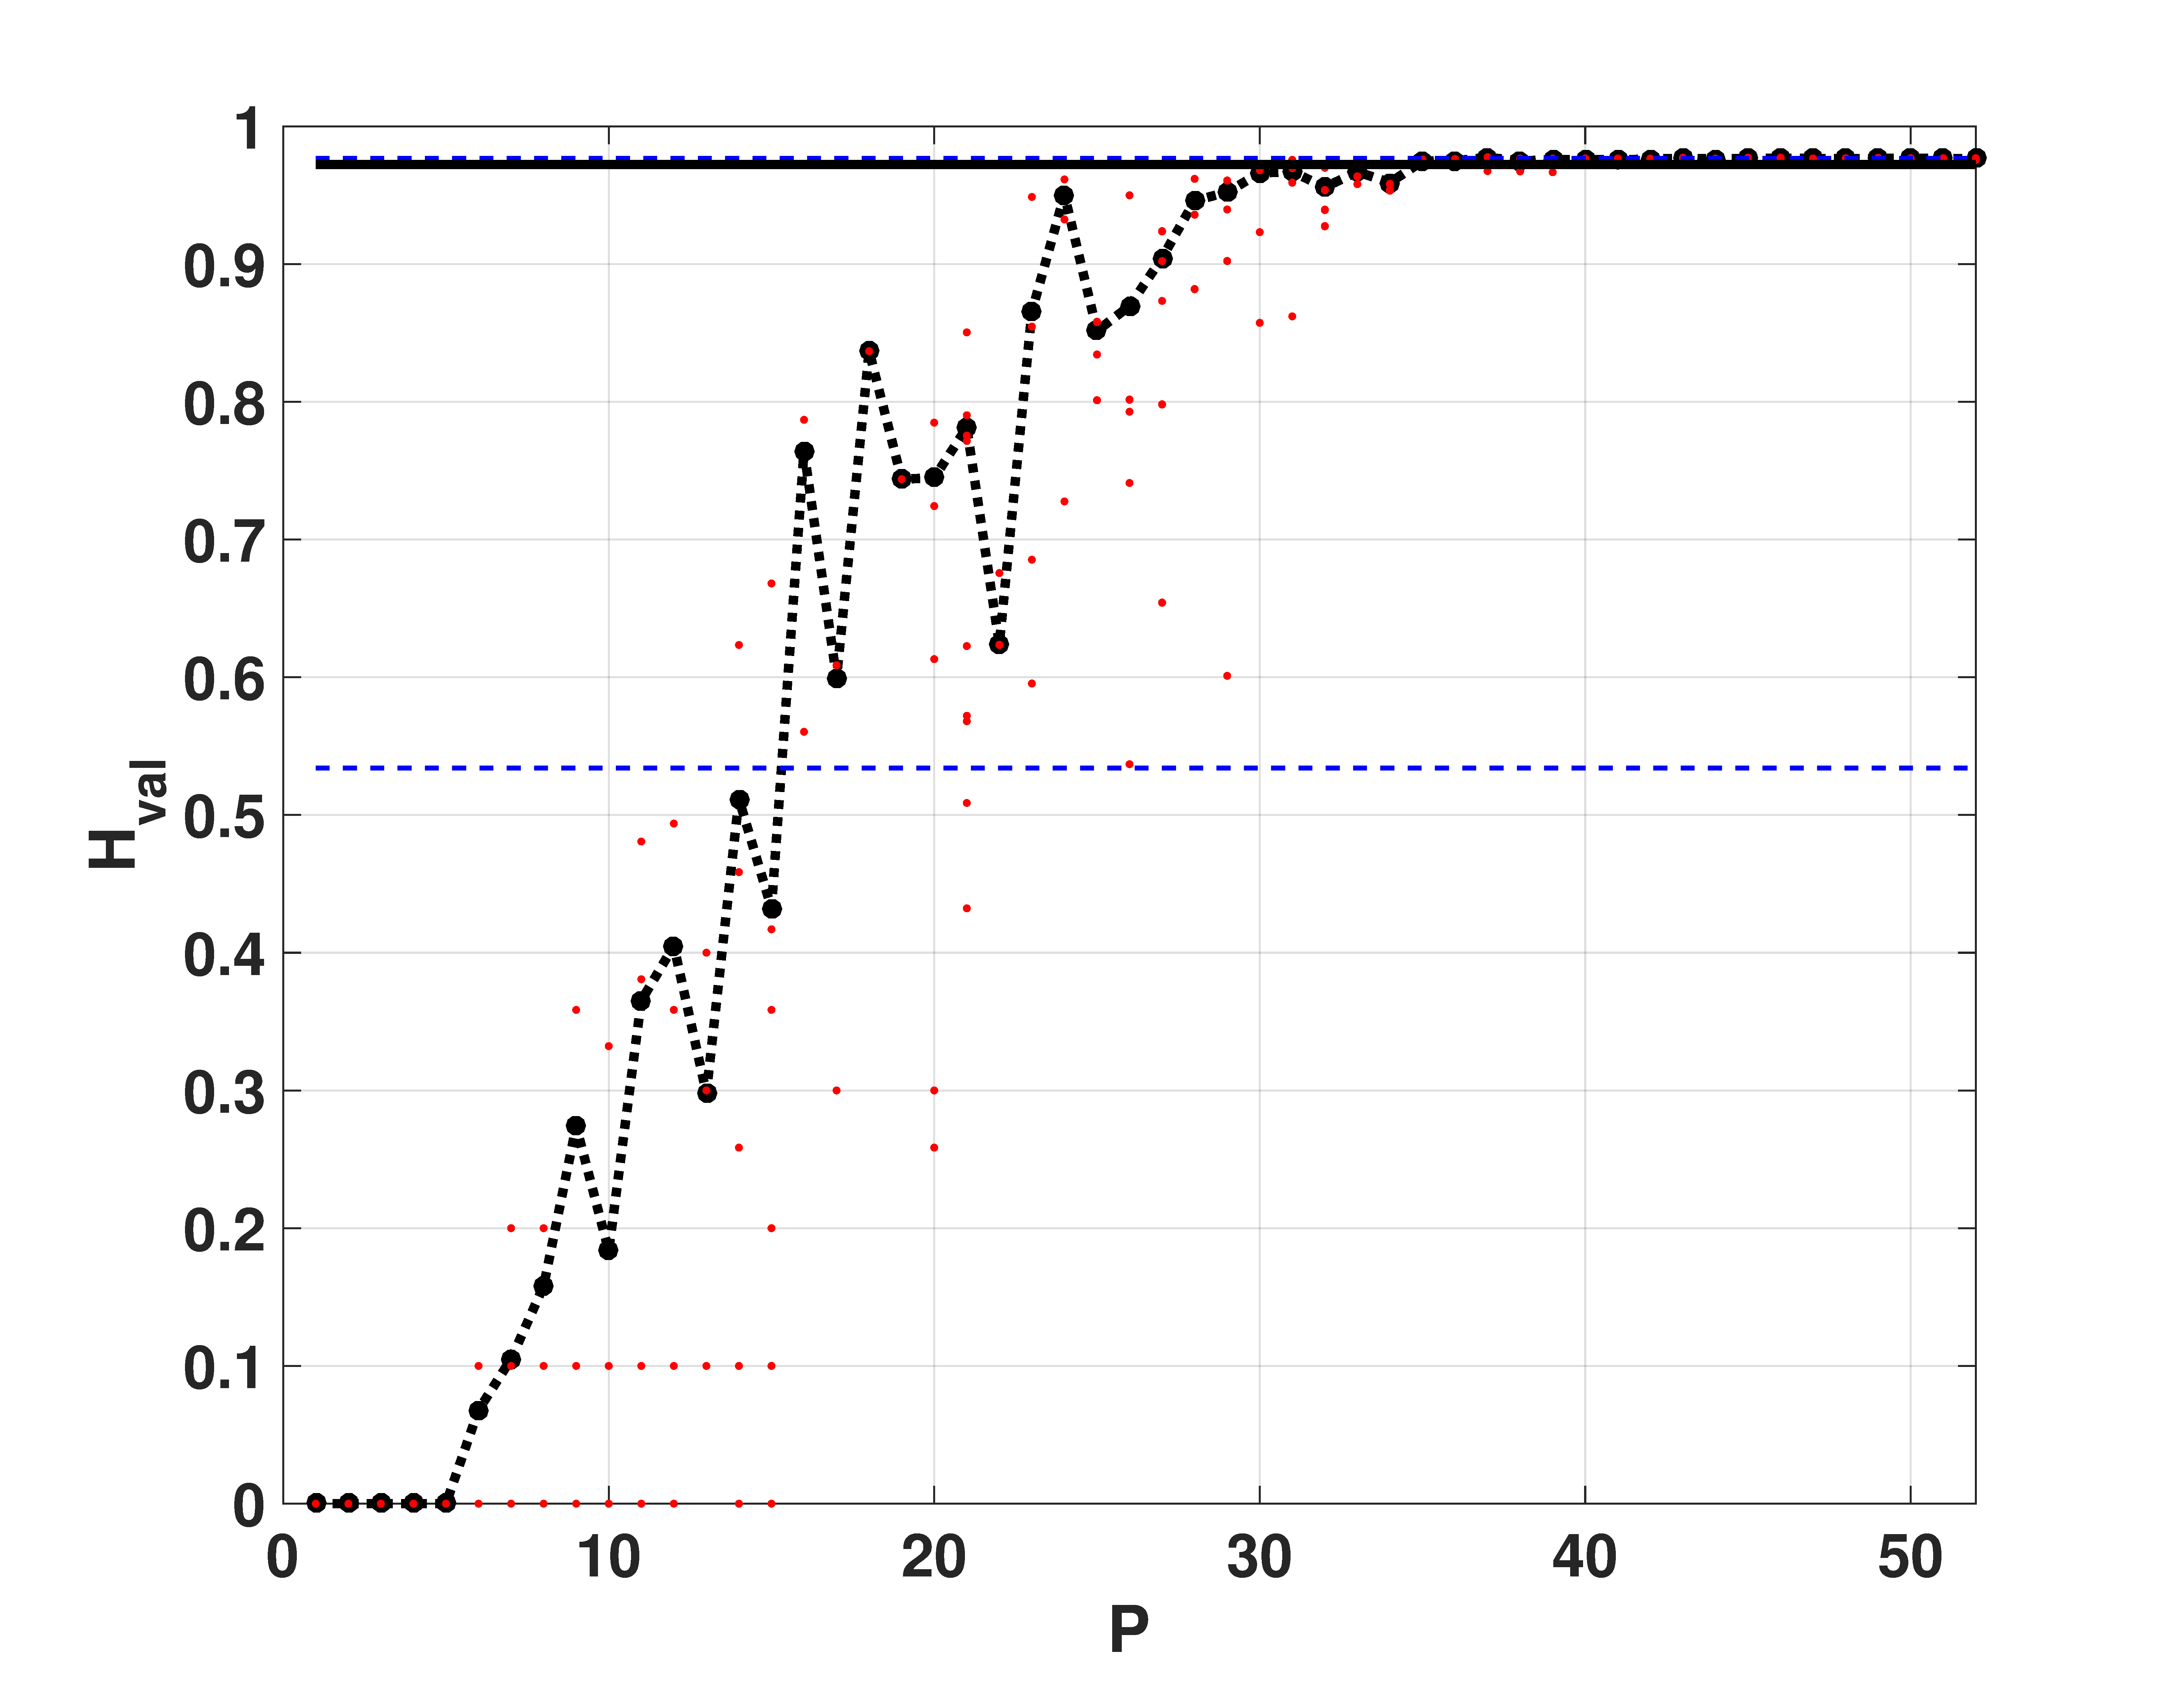
\includegraphics[width=.49\textwidth]{Hval_Switch}
	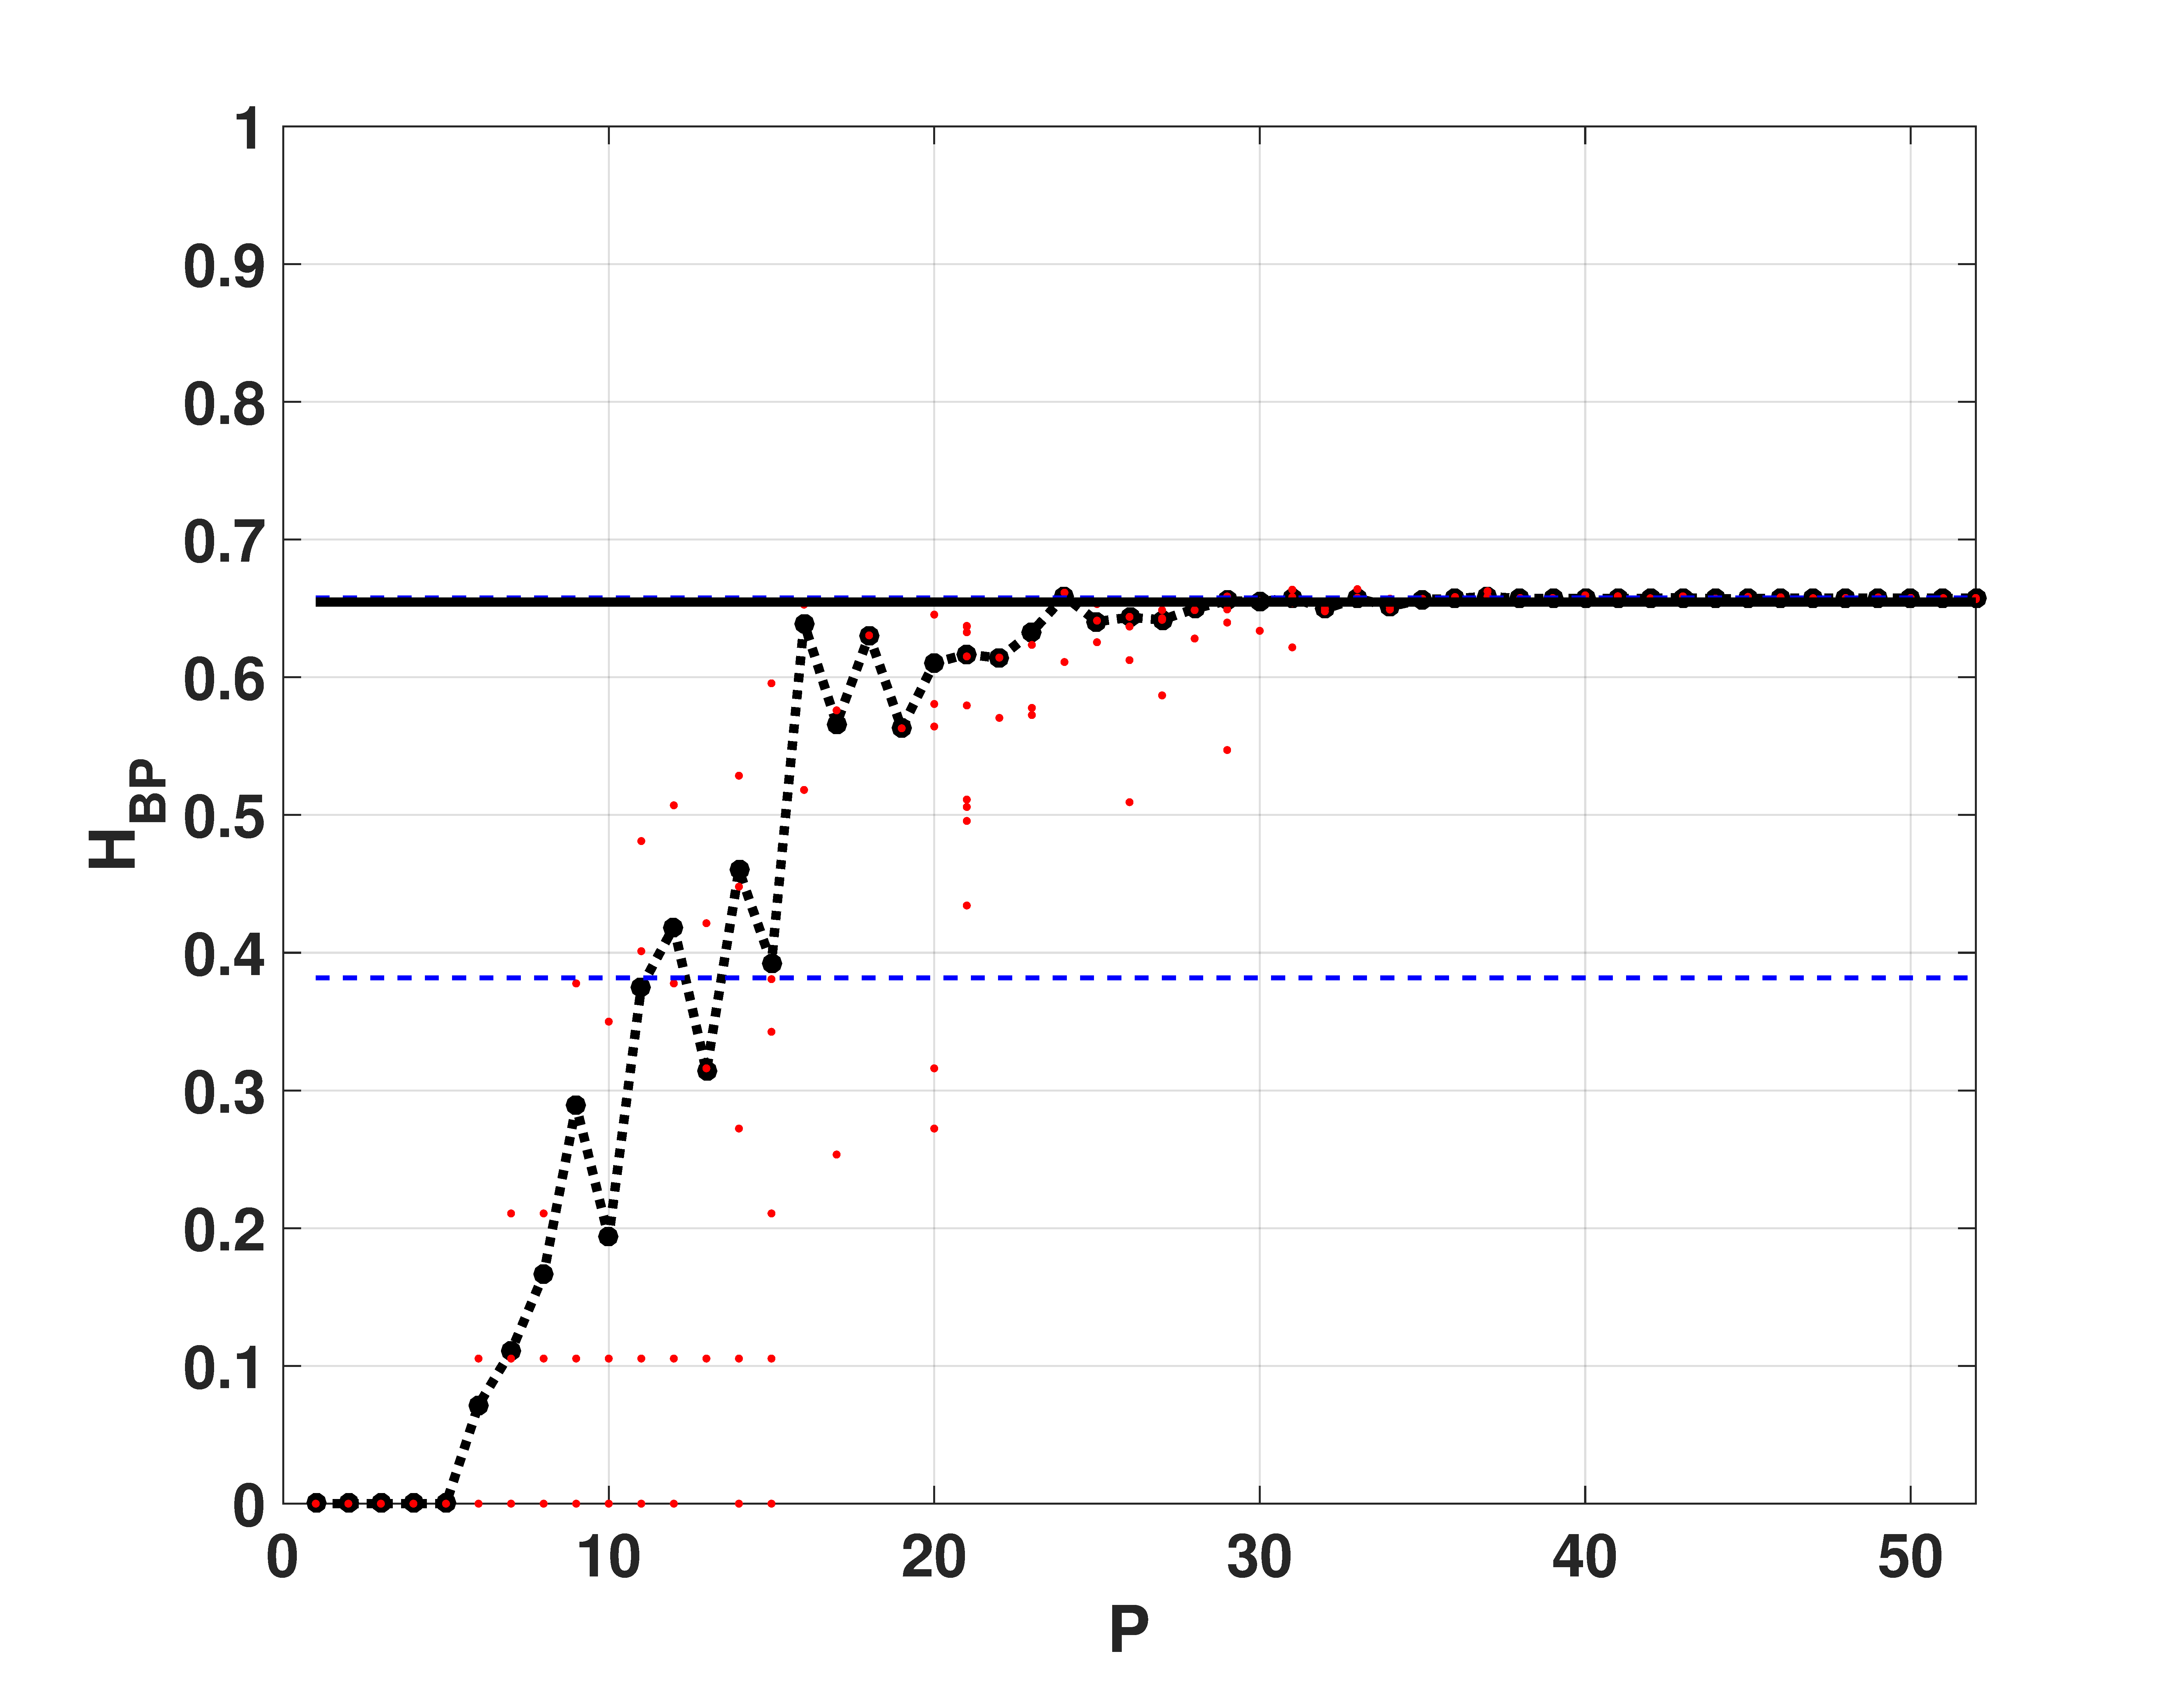
\includegraphics[width=.49\textwidth]{Hbp_Switch}
	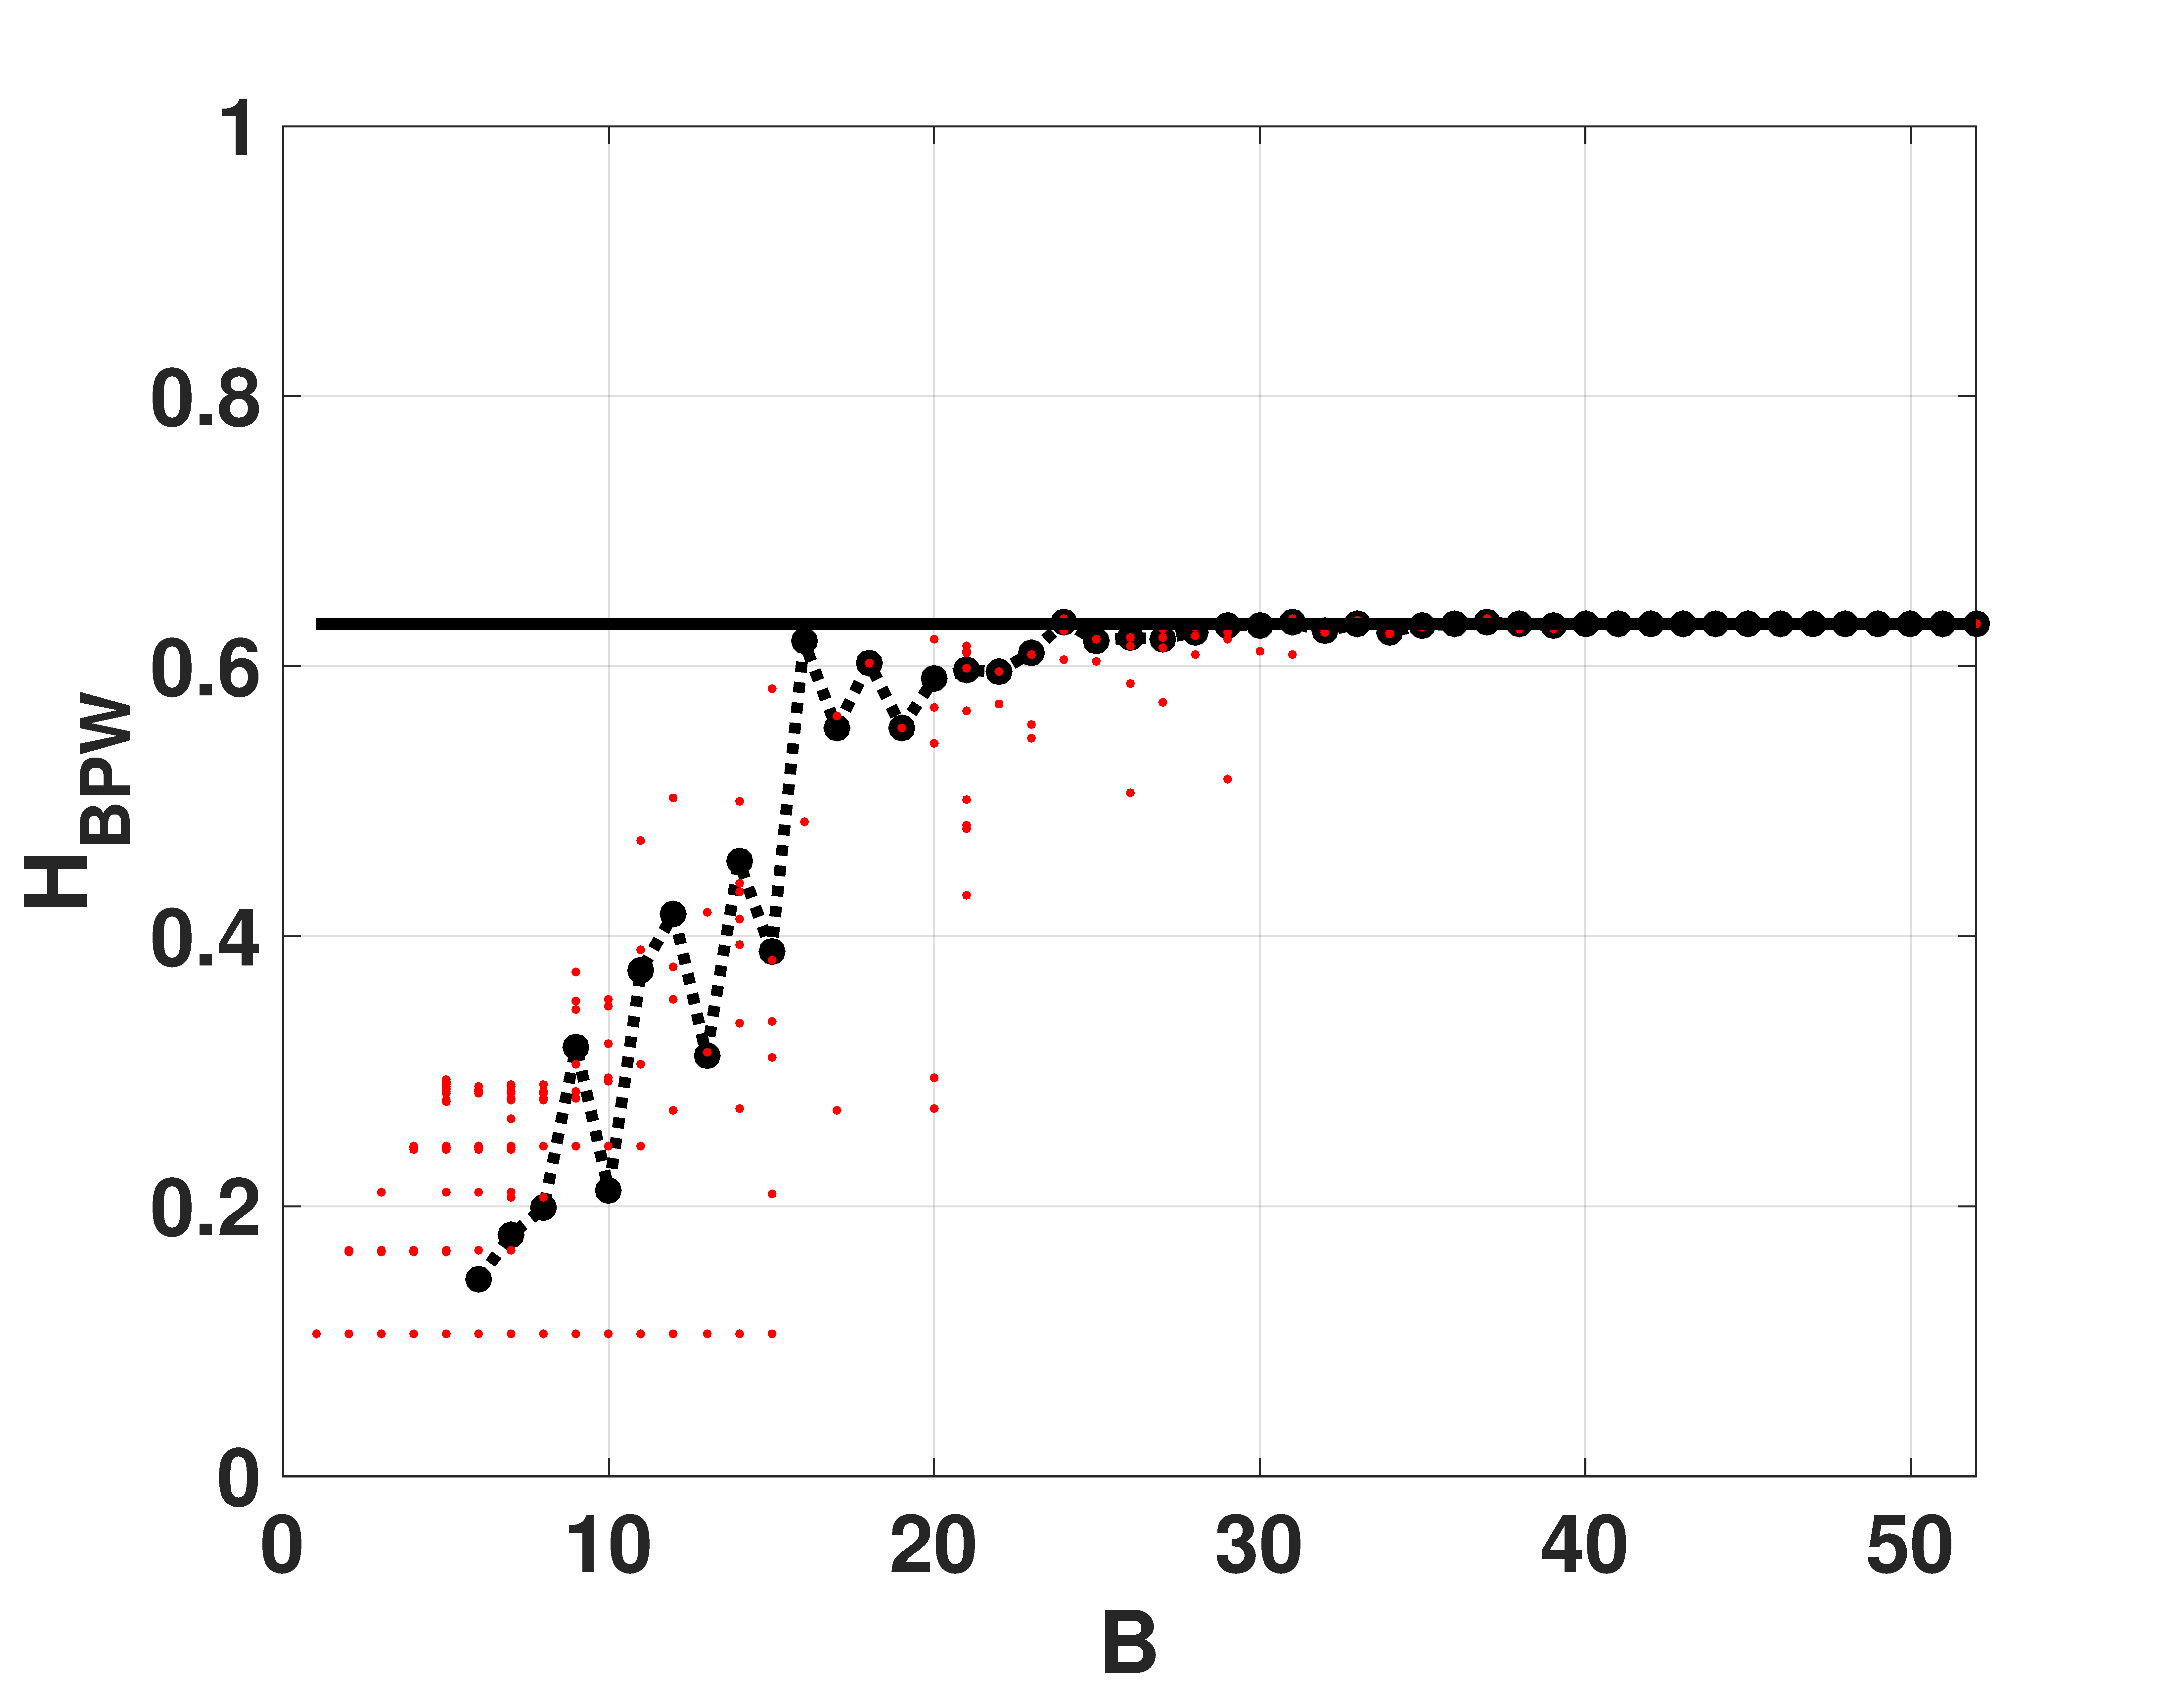
\includegraphics[width=.49\textwidth]{Hbpw_Switch}
	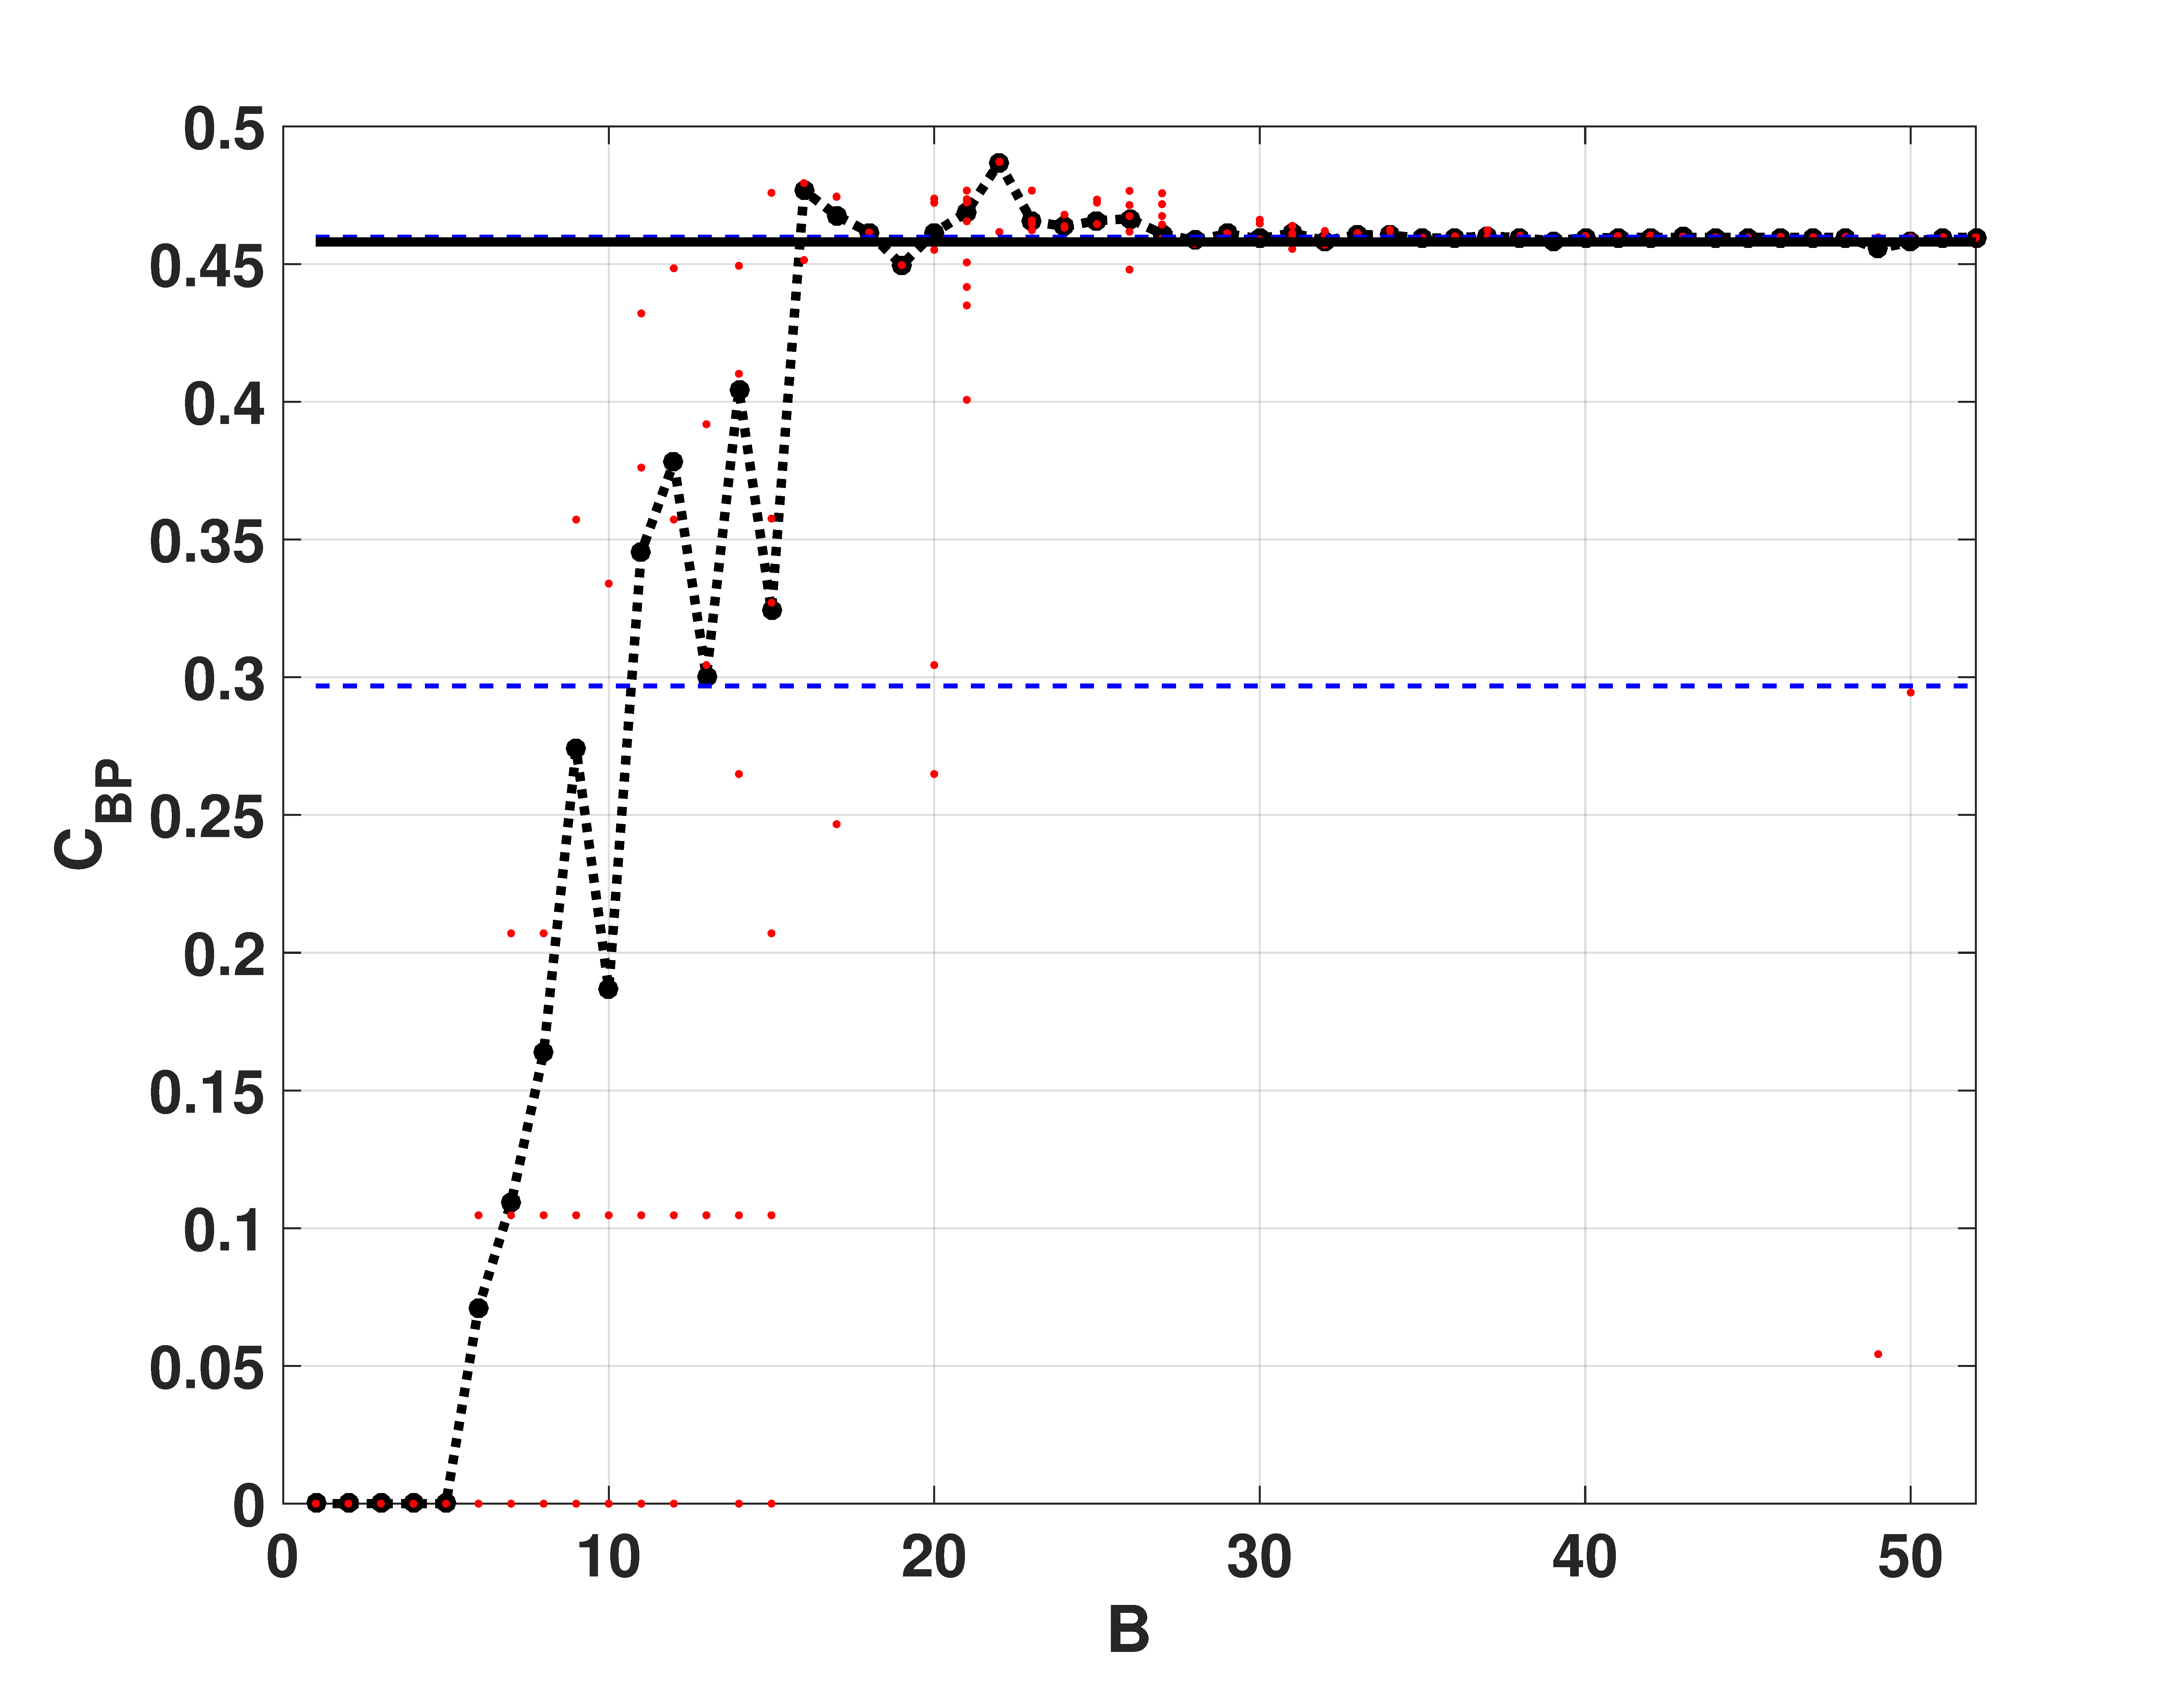
\includegraphics[width=.49\textwidth]{Cbp_Switch}
	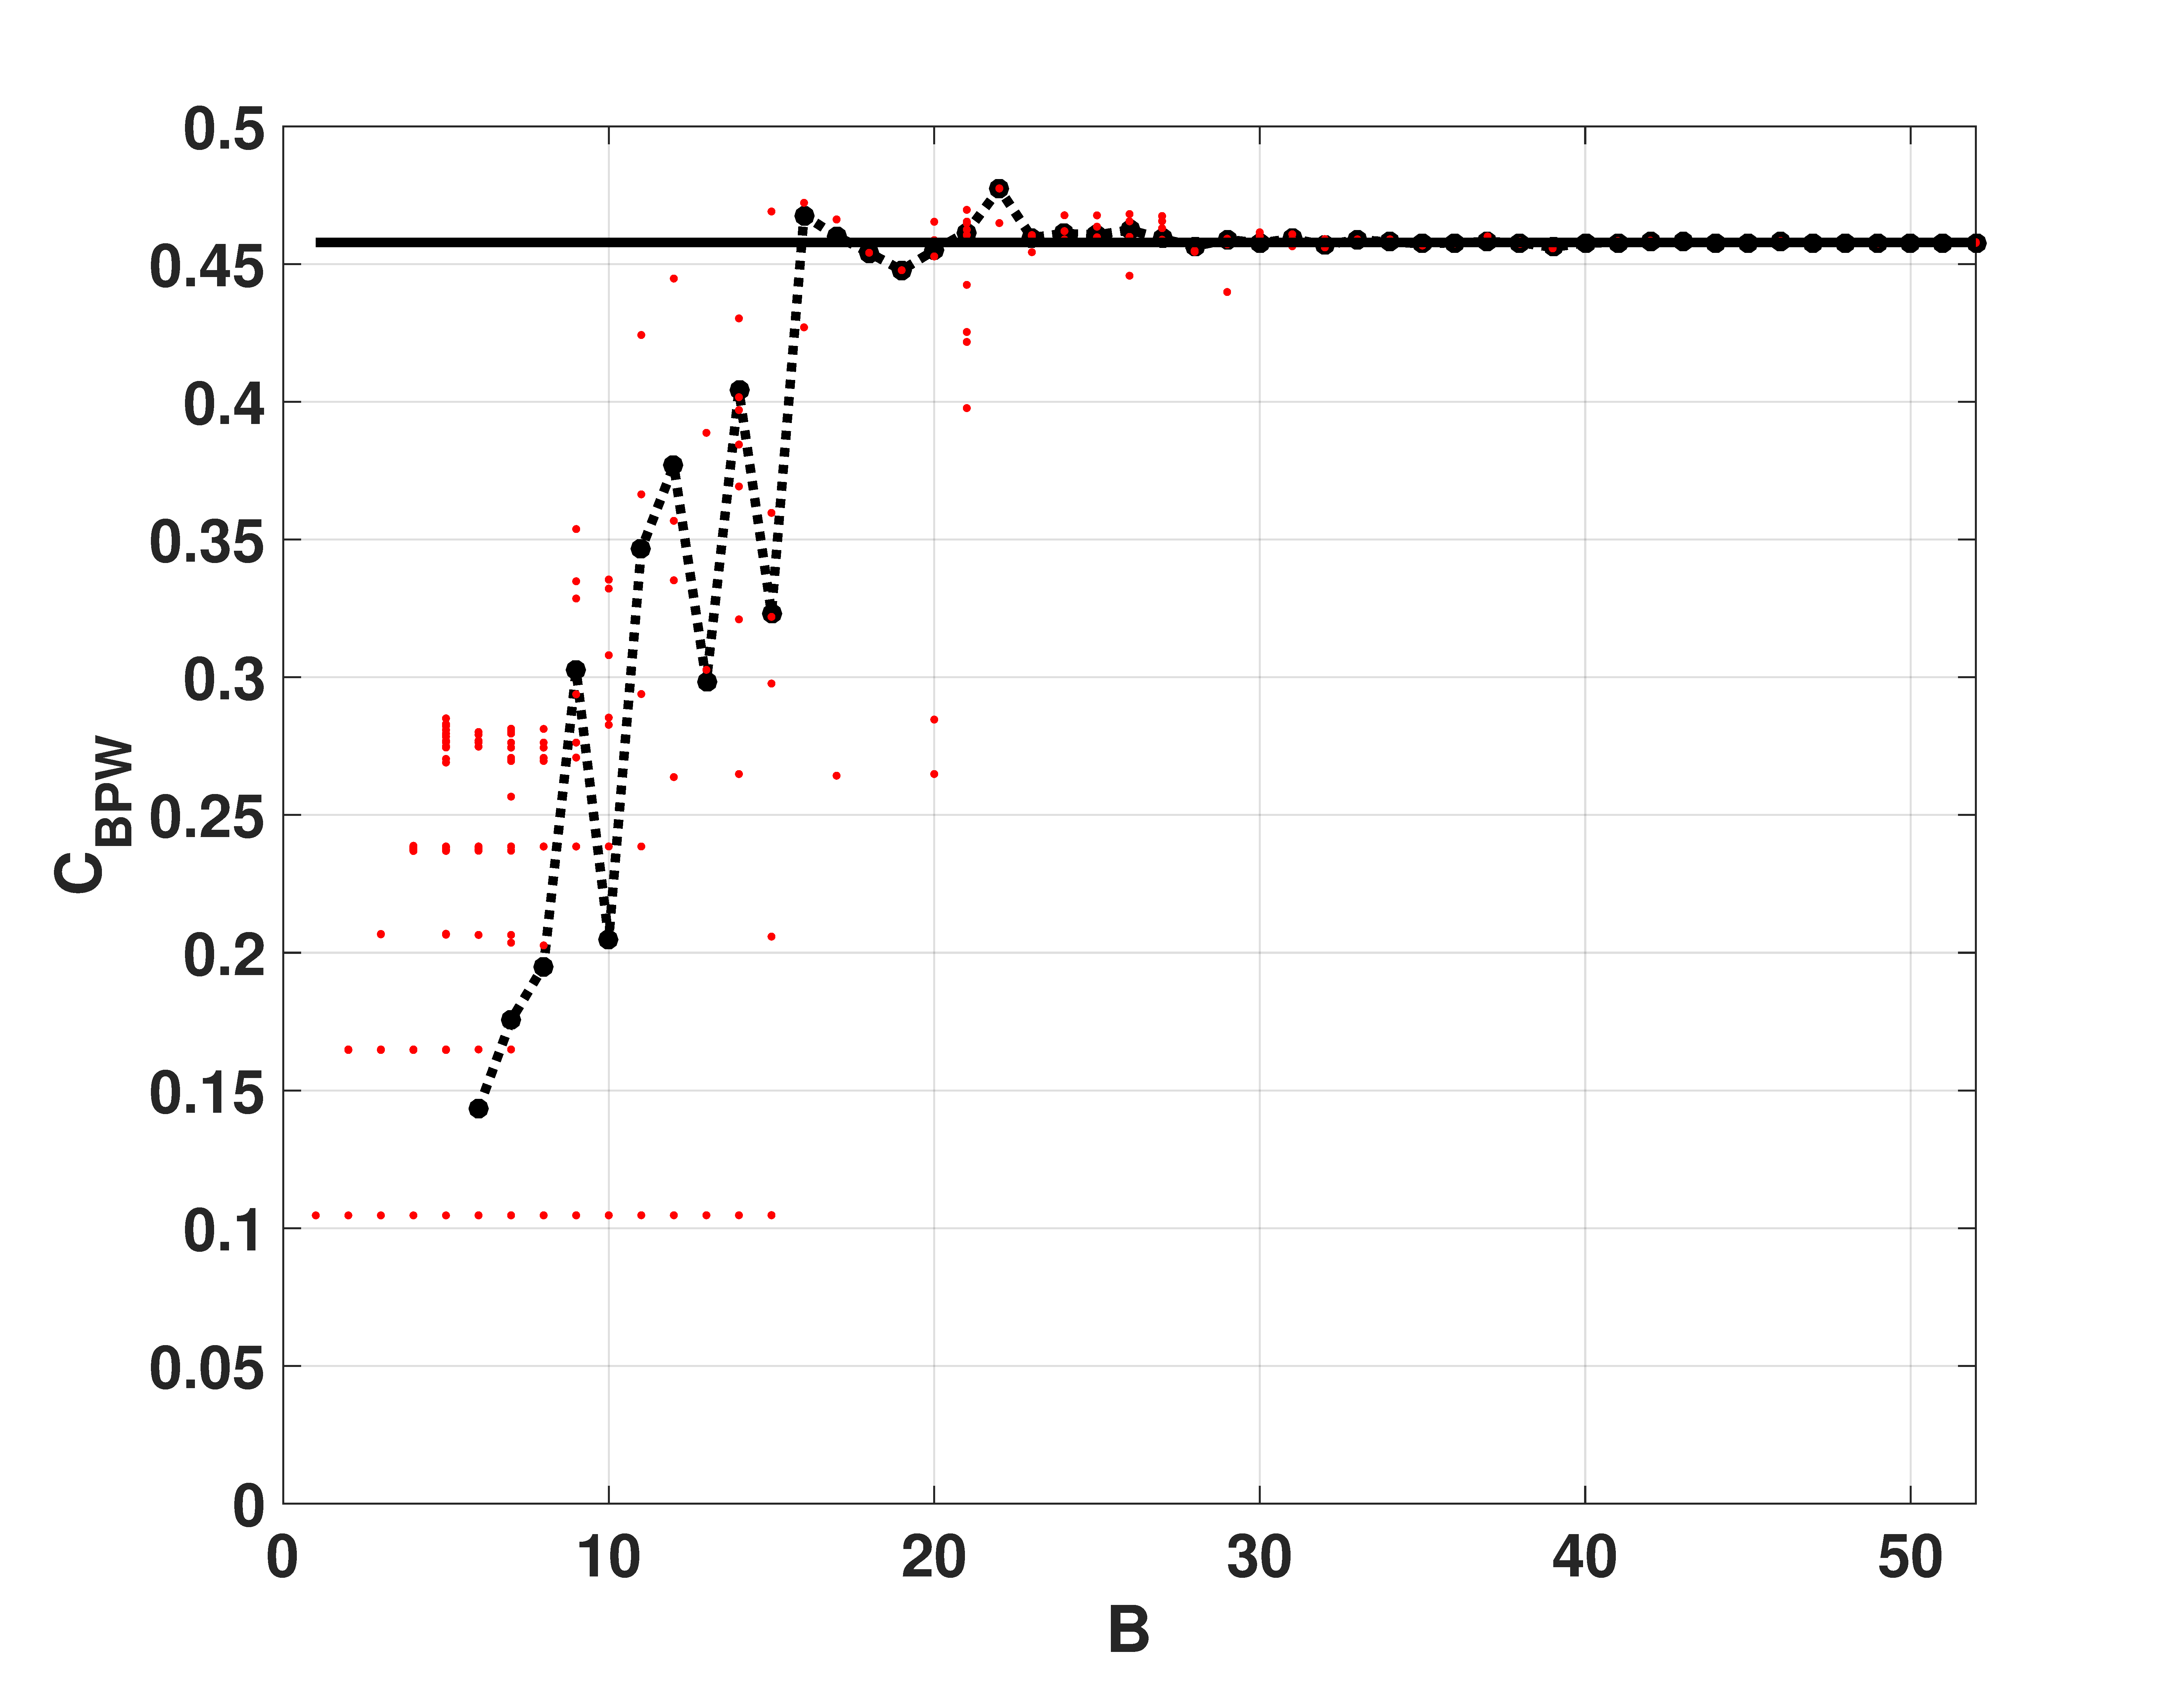
\includegraphics[width=.49\textwidth]{Cbpw_Switch}
	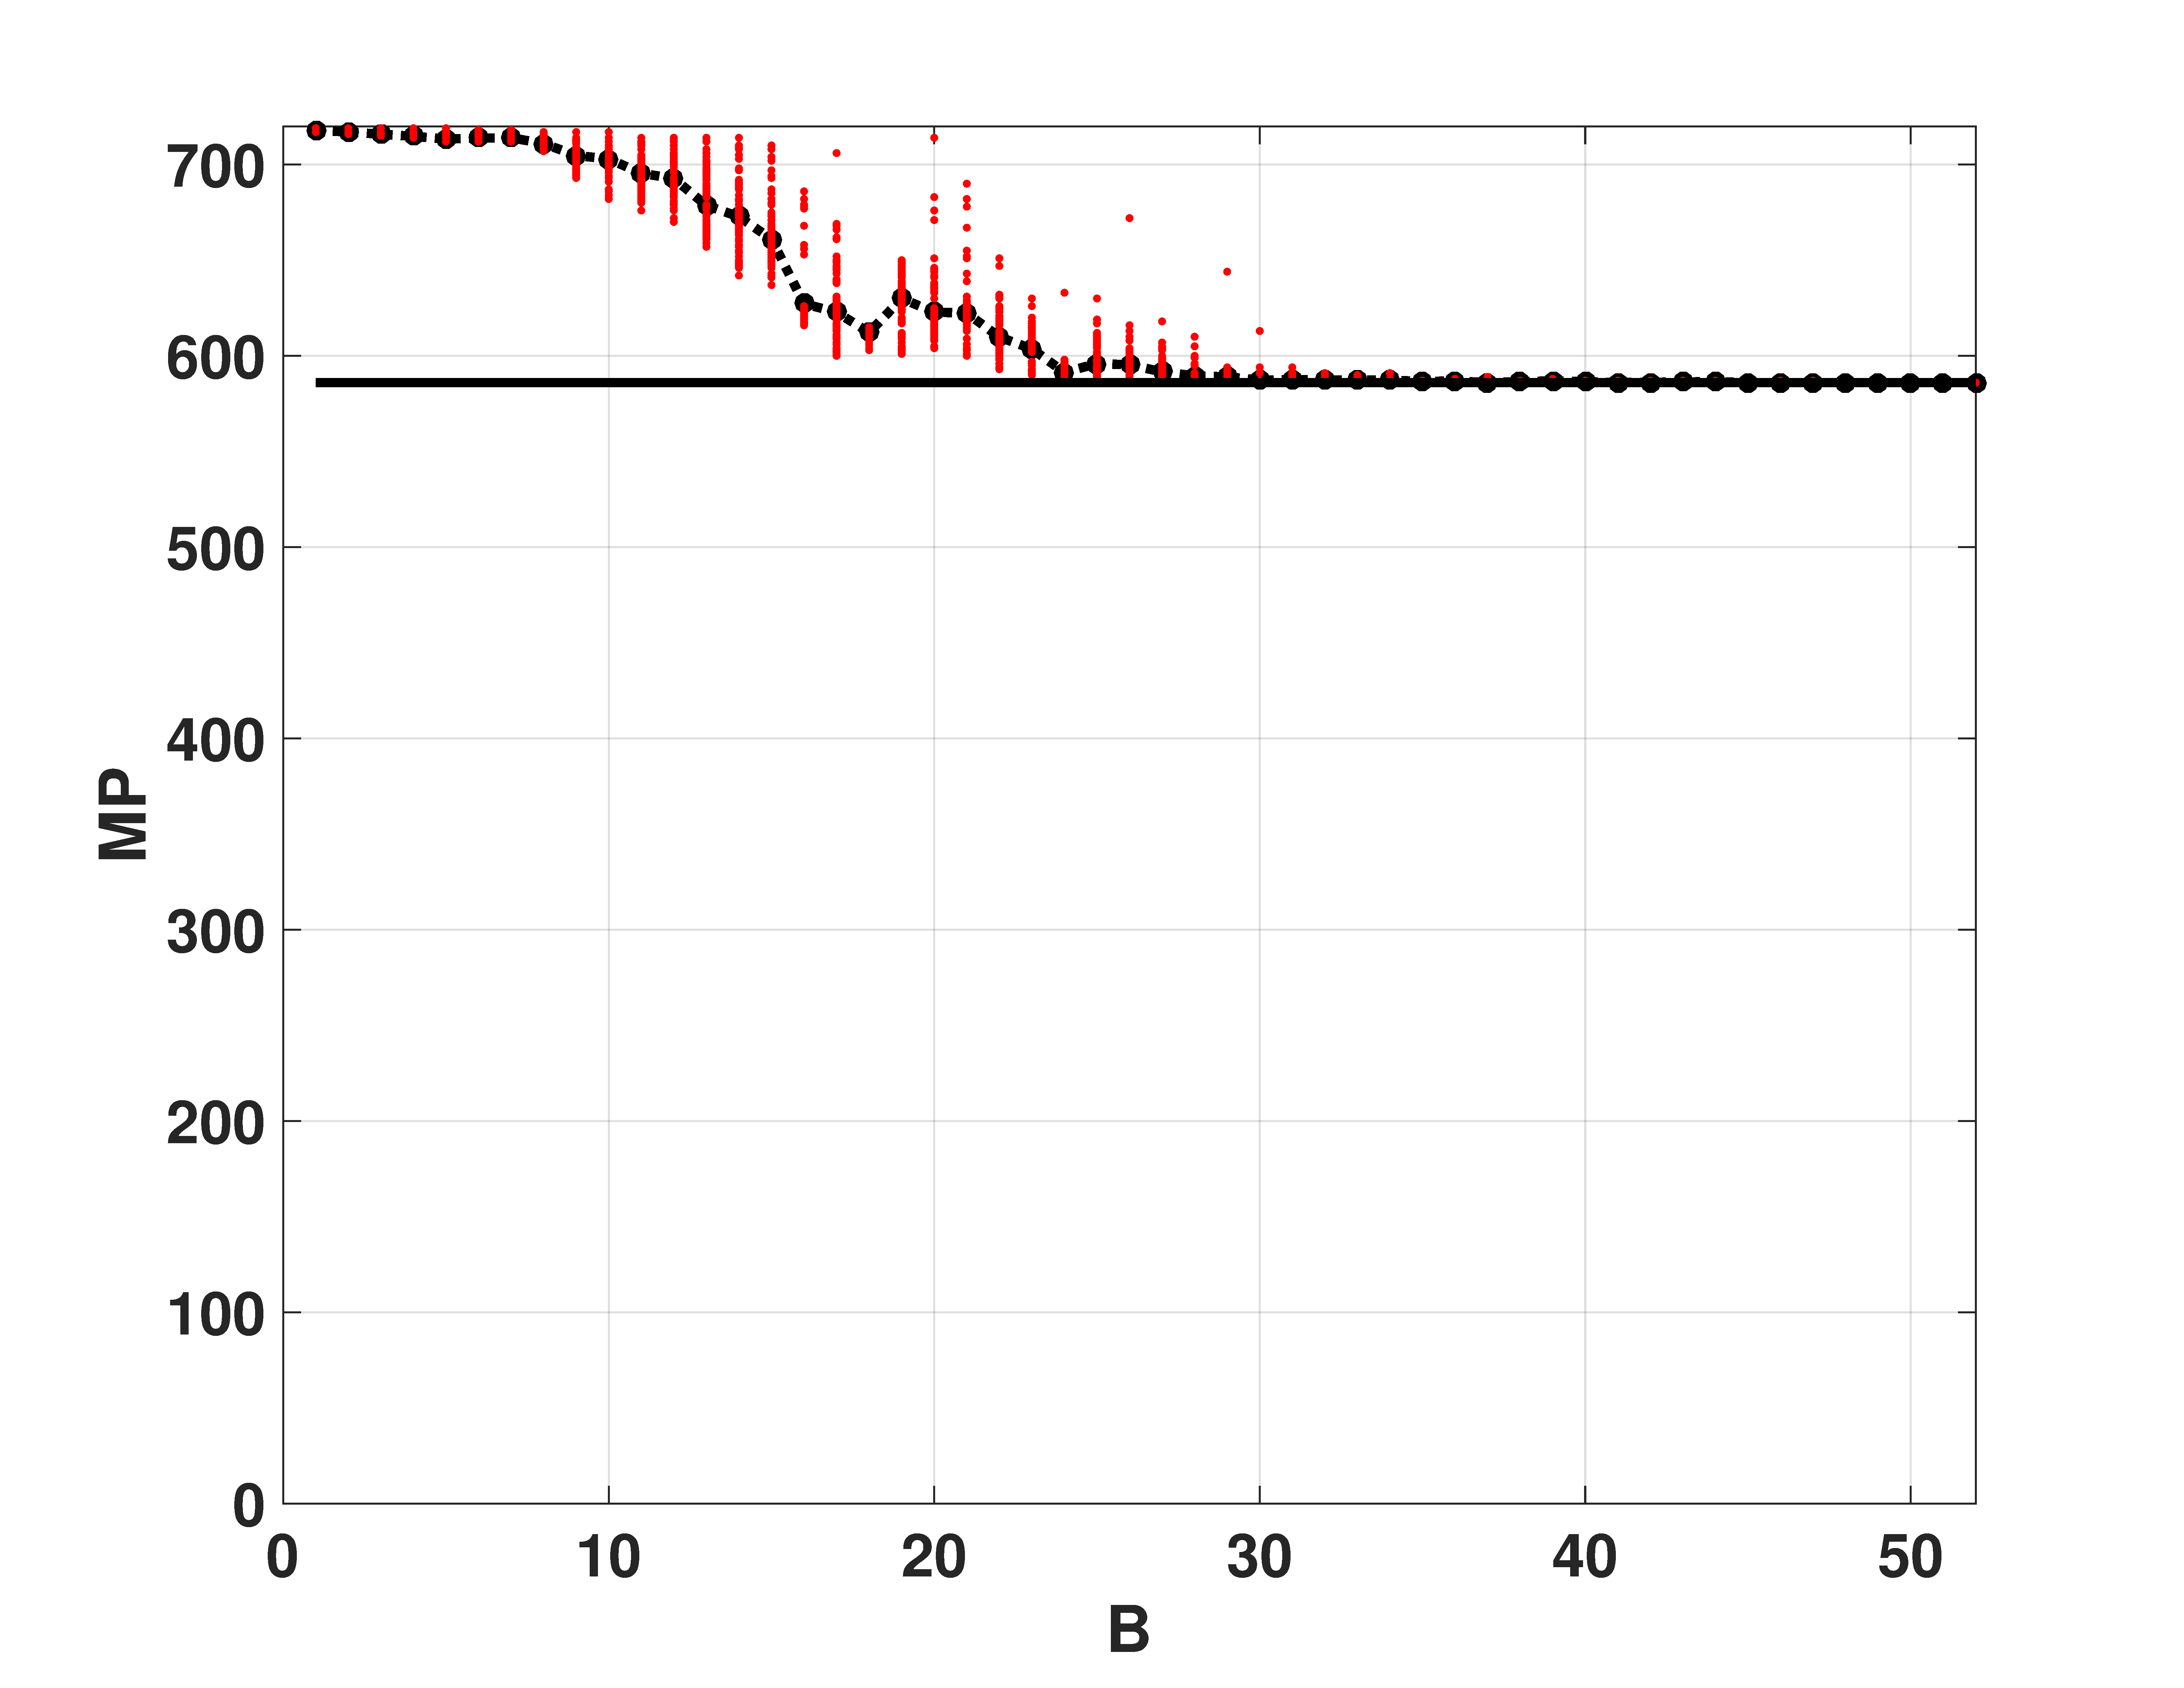
\includegraphics[width=.49\textwidth]{MP_Switch}
	\caption{Statistical properties of the SWITCH map (a) $H_{val}$ vs $B$ (b) $H_{BP}$ vs $B$ (c) $C_{BP}$ vs $B$ (d) $MP$ vs $B$.}
	\label{fig:SWITCH_QuantiB}
\end{figure}

Double entropy plane $H_{val}$ vs $H_{BP}$ is showed in Fig. \ref{fig:SWITCH_HH}.
The point reached in this plane for SWITCH map is similar to that reached for LOG map.
The mixing is slight better in this case.

\textcolor{red}{TENDRÍA QUE SACAR MAS CONCLUSIONES DE LOS PLANOS TENDRÍA QUE VERLAS EN LAS SERIES DE DATOS, ESPECIALMENTE EL PUNTO ESE QUE DA CORRIDO}

\begin{figure}
	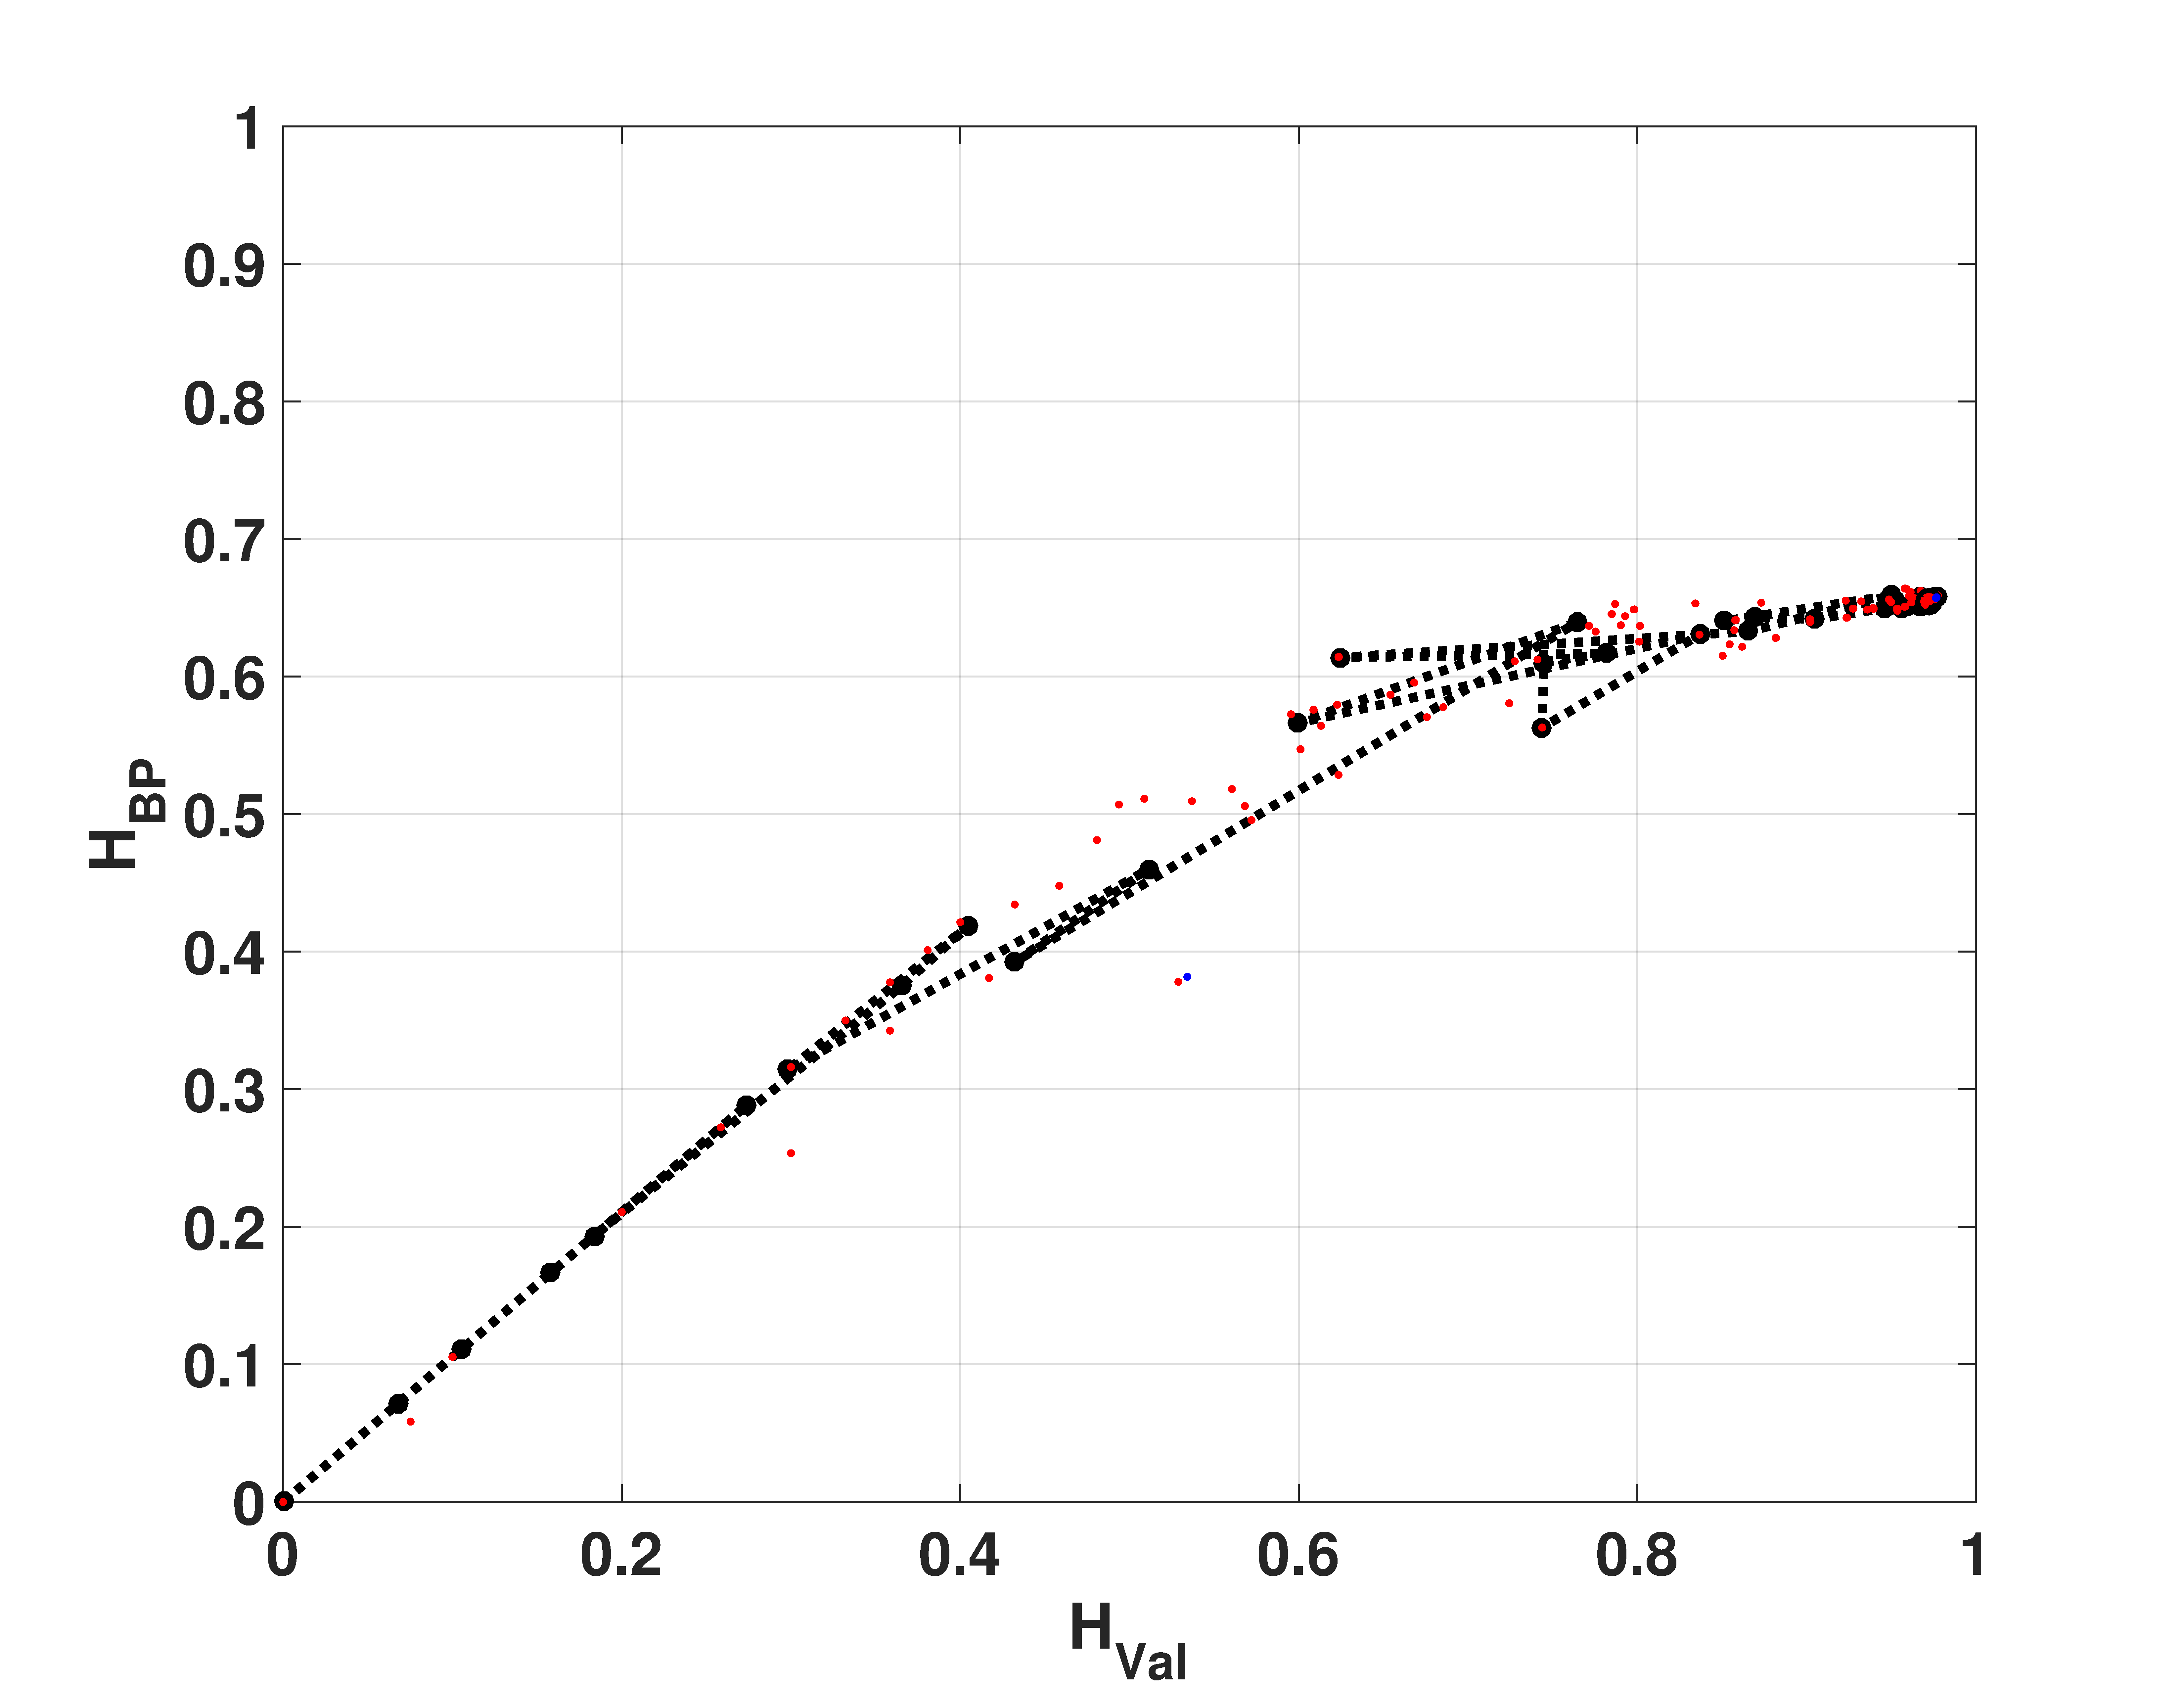
\includegraphics[width=.49\textwidth]{HbpHval_Switch}
	\caption{Evolution of statistical properties in double entropy plane of SWITCH map using binary representation: (a) $H_{val}$ vs $H_{BP}$ (b) $H_{val}$ vs $H_{BPW}$.}
	\label{fig:SWITCH_HH}
\end{figure}

Entropy-complexity plane $C_{BP}$ vs $H_{BP}$ is showed in Fig. \ref{fig:SWITCH_HC}.
If we compare with the same plane in the case of LOG (Fig. \ref{fig:LOG_HC}. a.), $C_{BP}$ is lower for SWITCH, this fact shows a more random behaviour.

\begin{figure}
	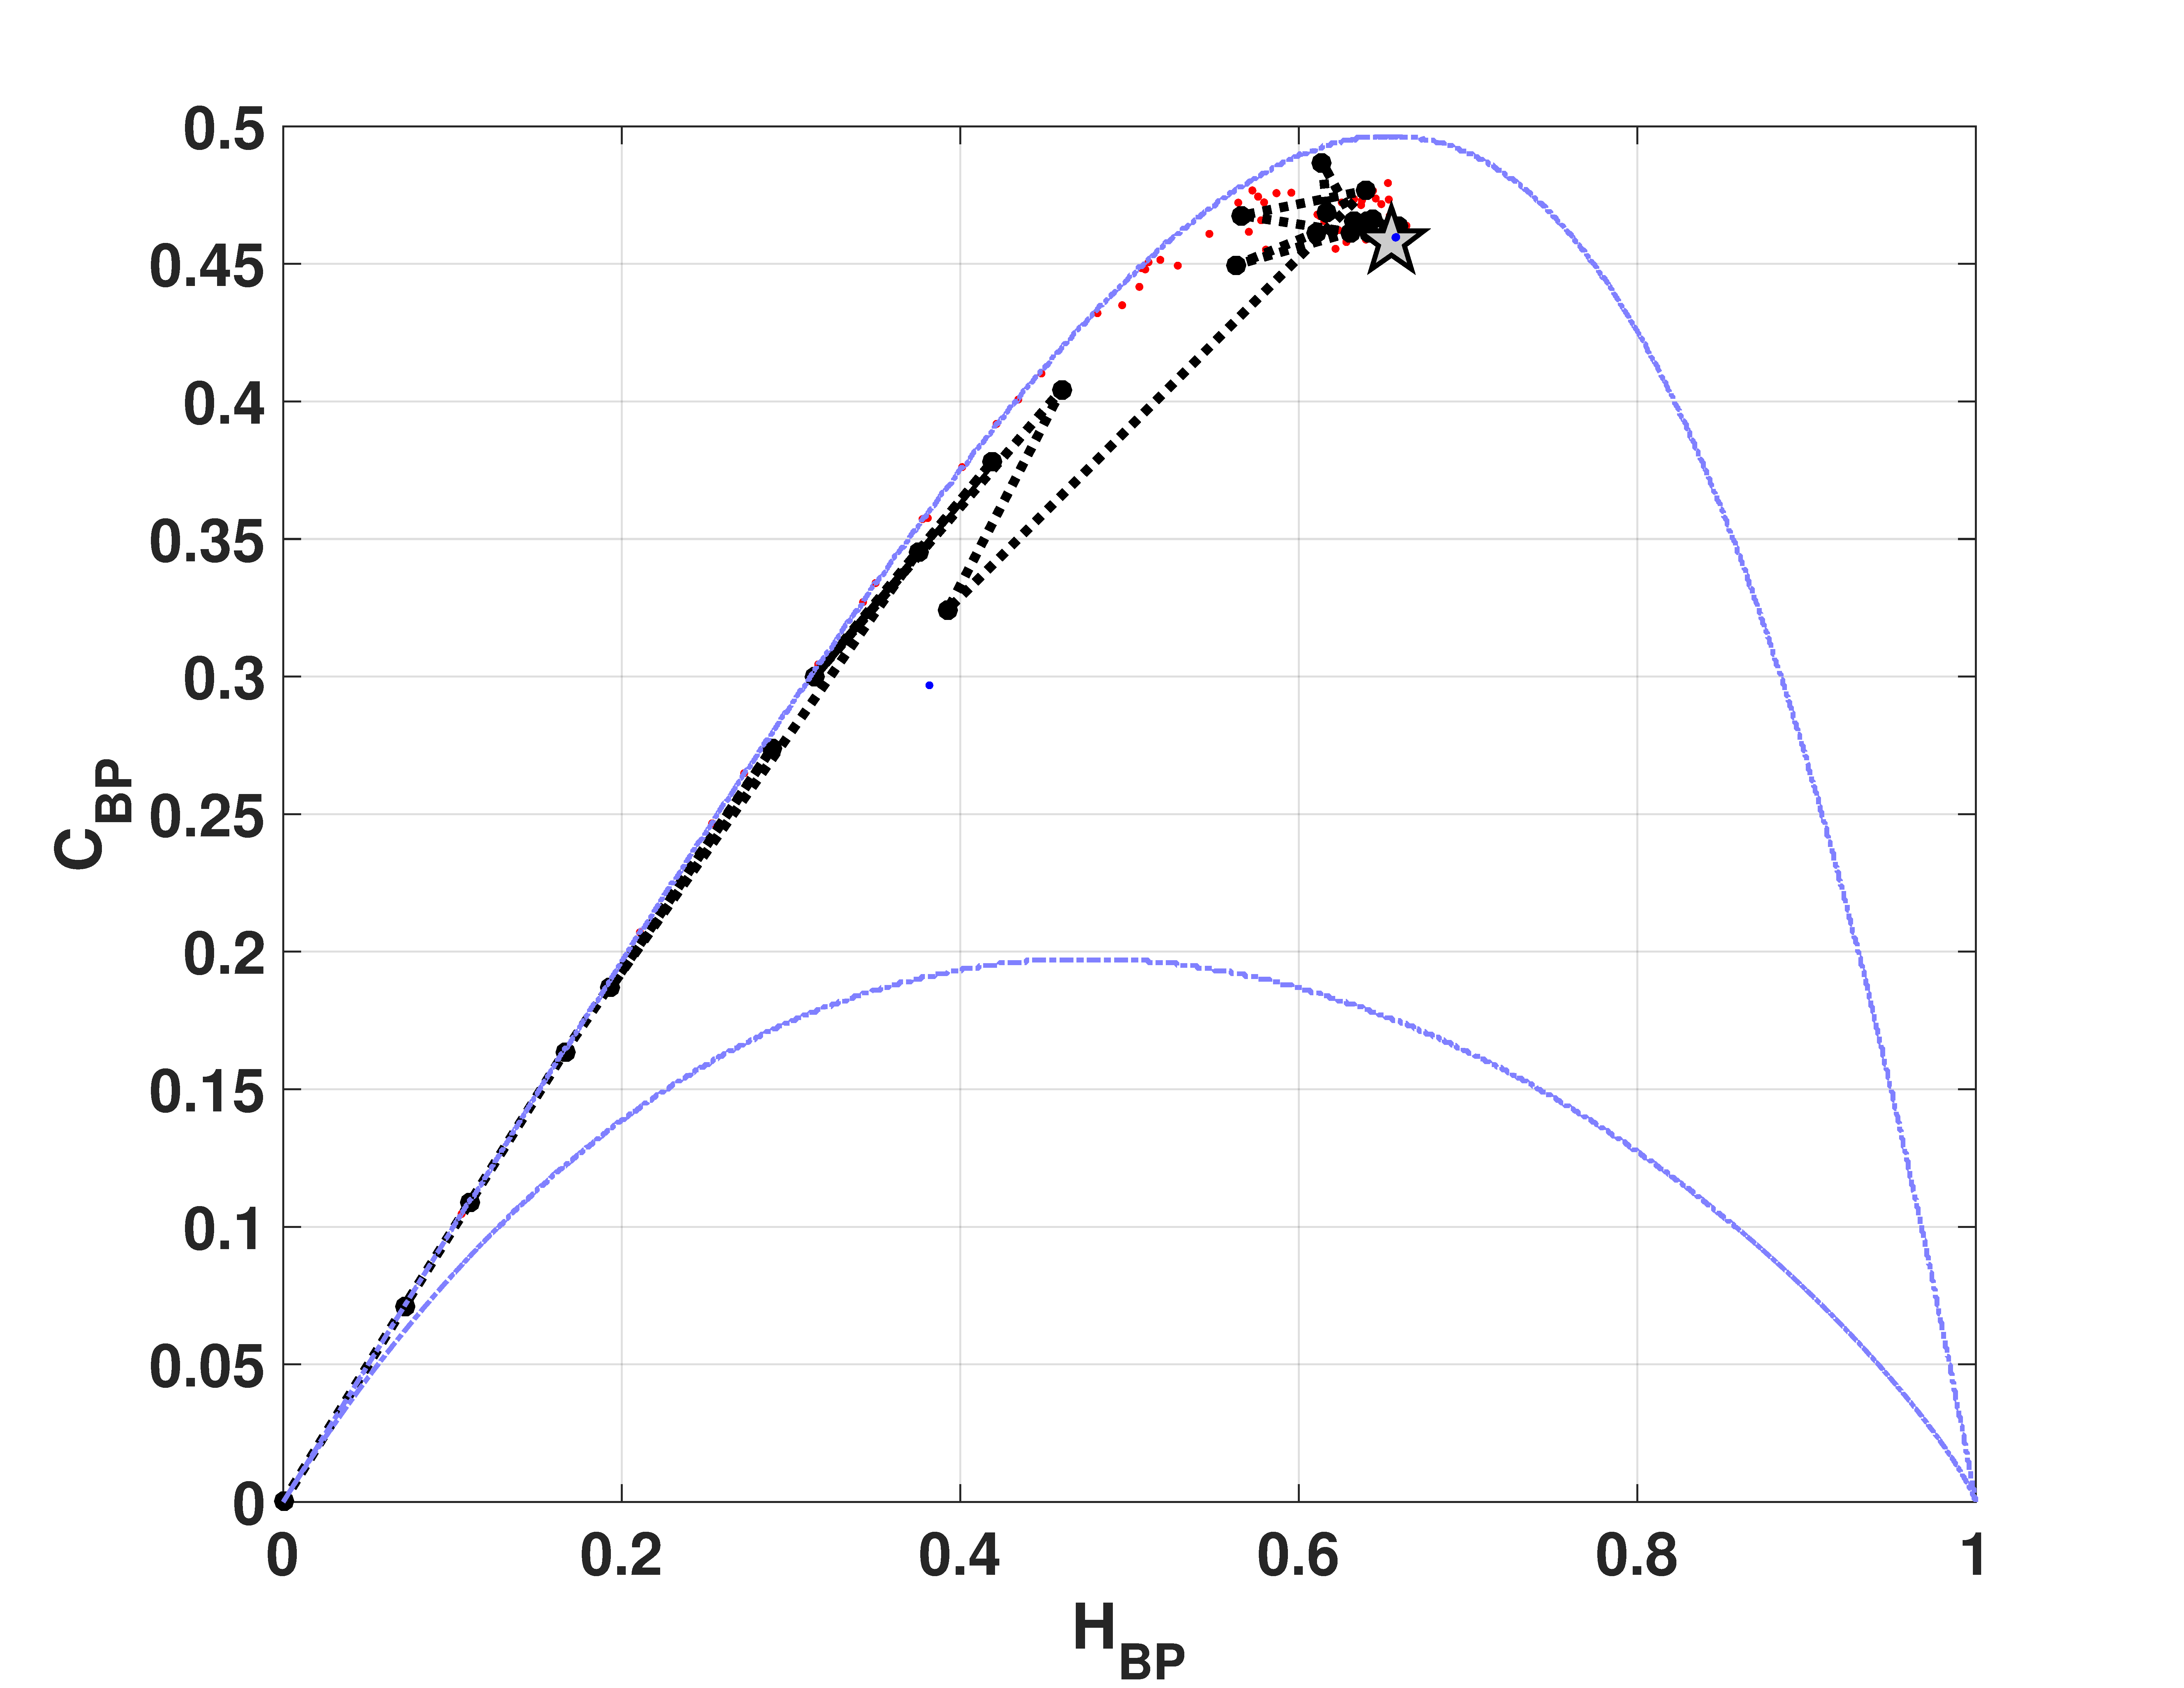
\includegraphics[width=.49\textwidth]{CbpHbp_Switch}
	\caption{Evolution of statistical properties in entropy-complexity plane of SWITCH map: $C_{BP}$ vs $H_{BP}$.}
	\label{fig:SWITCH_HC}
\end{figure}

\subsubsection{EVEN and ODD} \label{sssec:skipp}

In Figures \ref{fig:Hval_Even} and \ref{fig:Hval_Odd} we can see that quantifiers related to the normalized histogram of values slightly degrades with the skipping procedure.
For example $\left\langle H_{hist}\right\rangle $ reduces from $0.9722$ without skipping to $0.9459$ for EVEN and $0.9706$ for ODD. 
This difference between EVEN and ODD in floating point is because a high dispersion was obtained for $H_{hist}$, $H_{BP}$ and $C_{BP}$ but not for $H_{BPW}$ or $C_{BPW}$.

Figures \ref{fig:Hbp_Even} to \ref{fig:MP_Even} and Figures \ref{fig:Hbp_Odd} to \ref{fig:MP_Odd} show the results of BP and BPW quantifiers for EVEN and ODD respectively.
Higher accuracy is required to achieve lower complexity than without using skipping.
From the MP point of view a great improvement is obtained using any of the skipping strategies but ODD is slightly better than EVEN.
Missing patterns are reduced to $MP = 118$ for EVEN and ODD, increasing the maximum allowed Bandt \& Pompe entropy that reaches the mean value $\left\langle H_{BP}\right\rangle  = 0.8381$ for EVEN, and $\left\langle H_{BP}\right\rangle  = 0.9094$.
The complexity is reduced to $\left\langle C_{BP}\right\rangle = 0.224$ for EVEN and $\left\langle C_{BP}\right\rangle = 0.282$ for ODD.
The minimum number of bits to converge to this value is $B>40$ for both EVEN and ODD maps.
%
\begin{figure}[H]
	\centering
	\begin{subfigure}[b]{0.49\textwidth}
		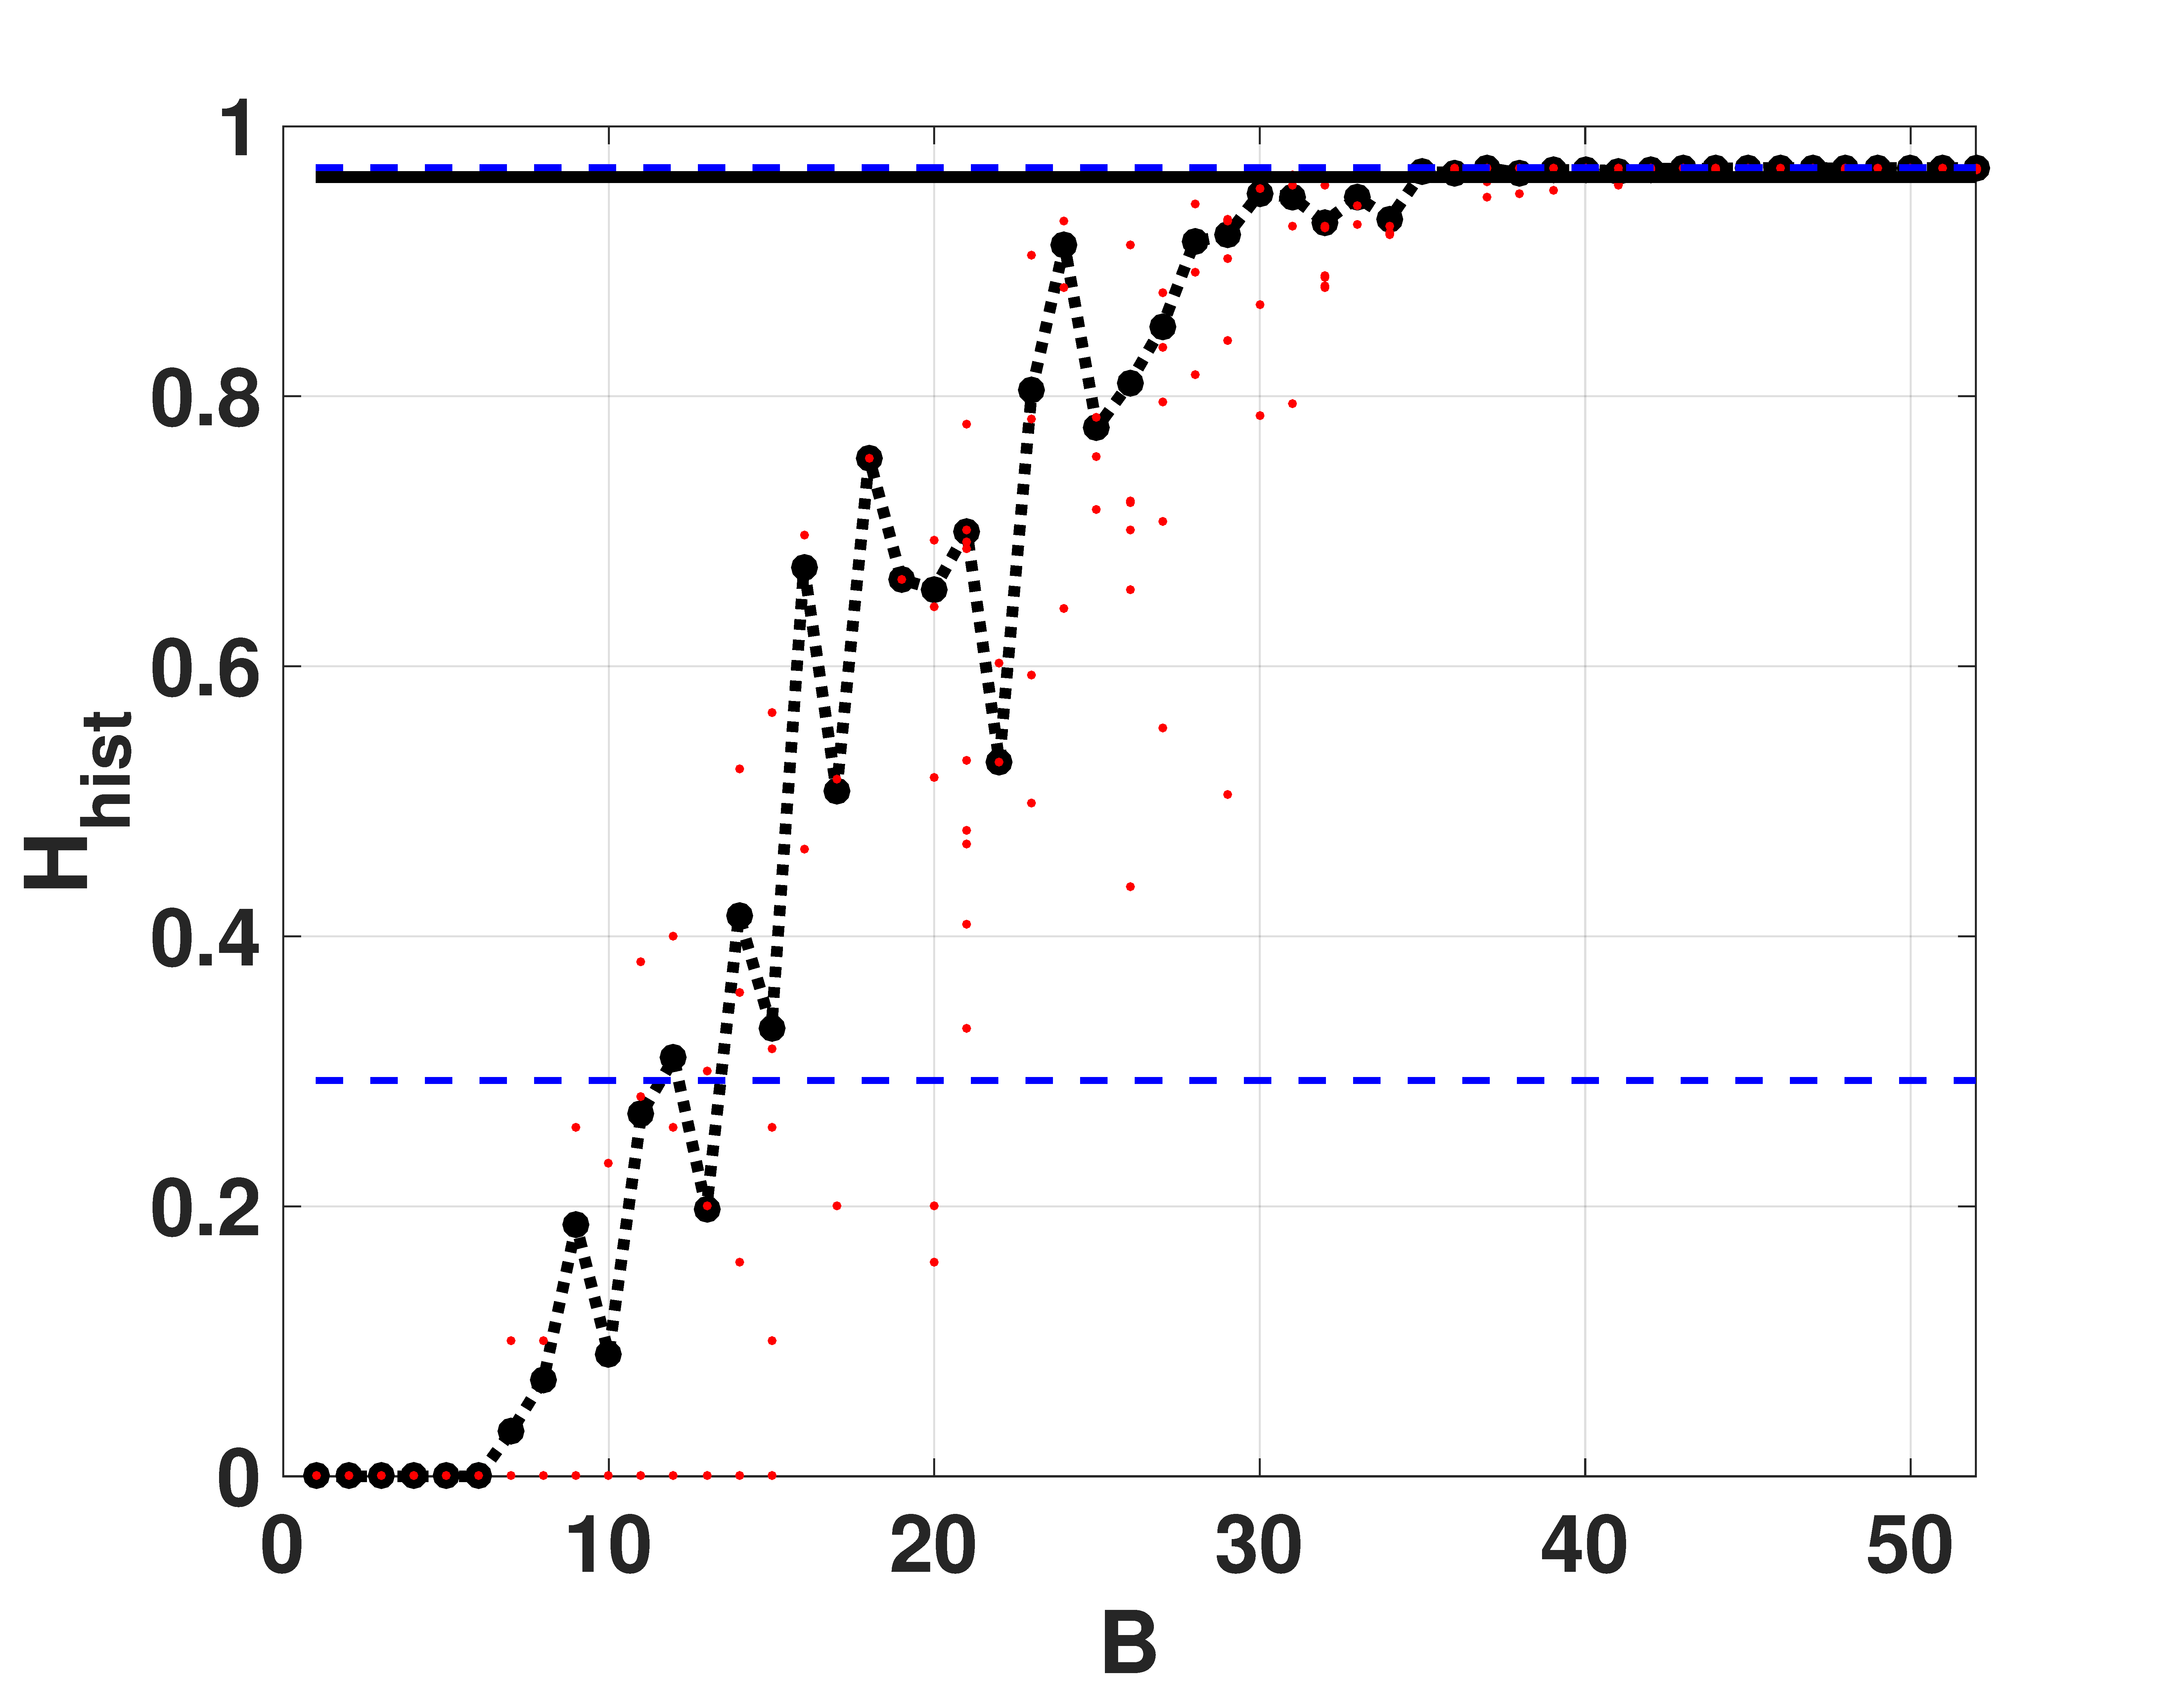
\includegraphics[width=\textwidth]{Hval_Even}
		\caption{$H_{hist}$ vs. $B$}
		\label{fig:Hval_Even}
	\end{subfigure}
	\begin{subfigure}[b]{0.49\textwidth}
		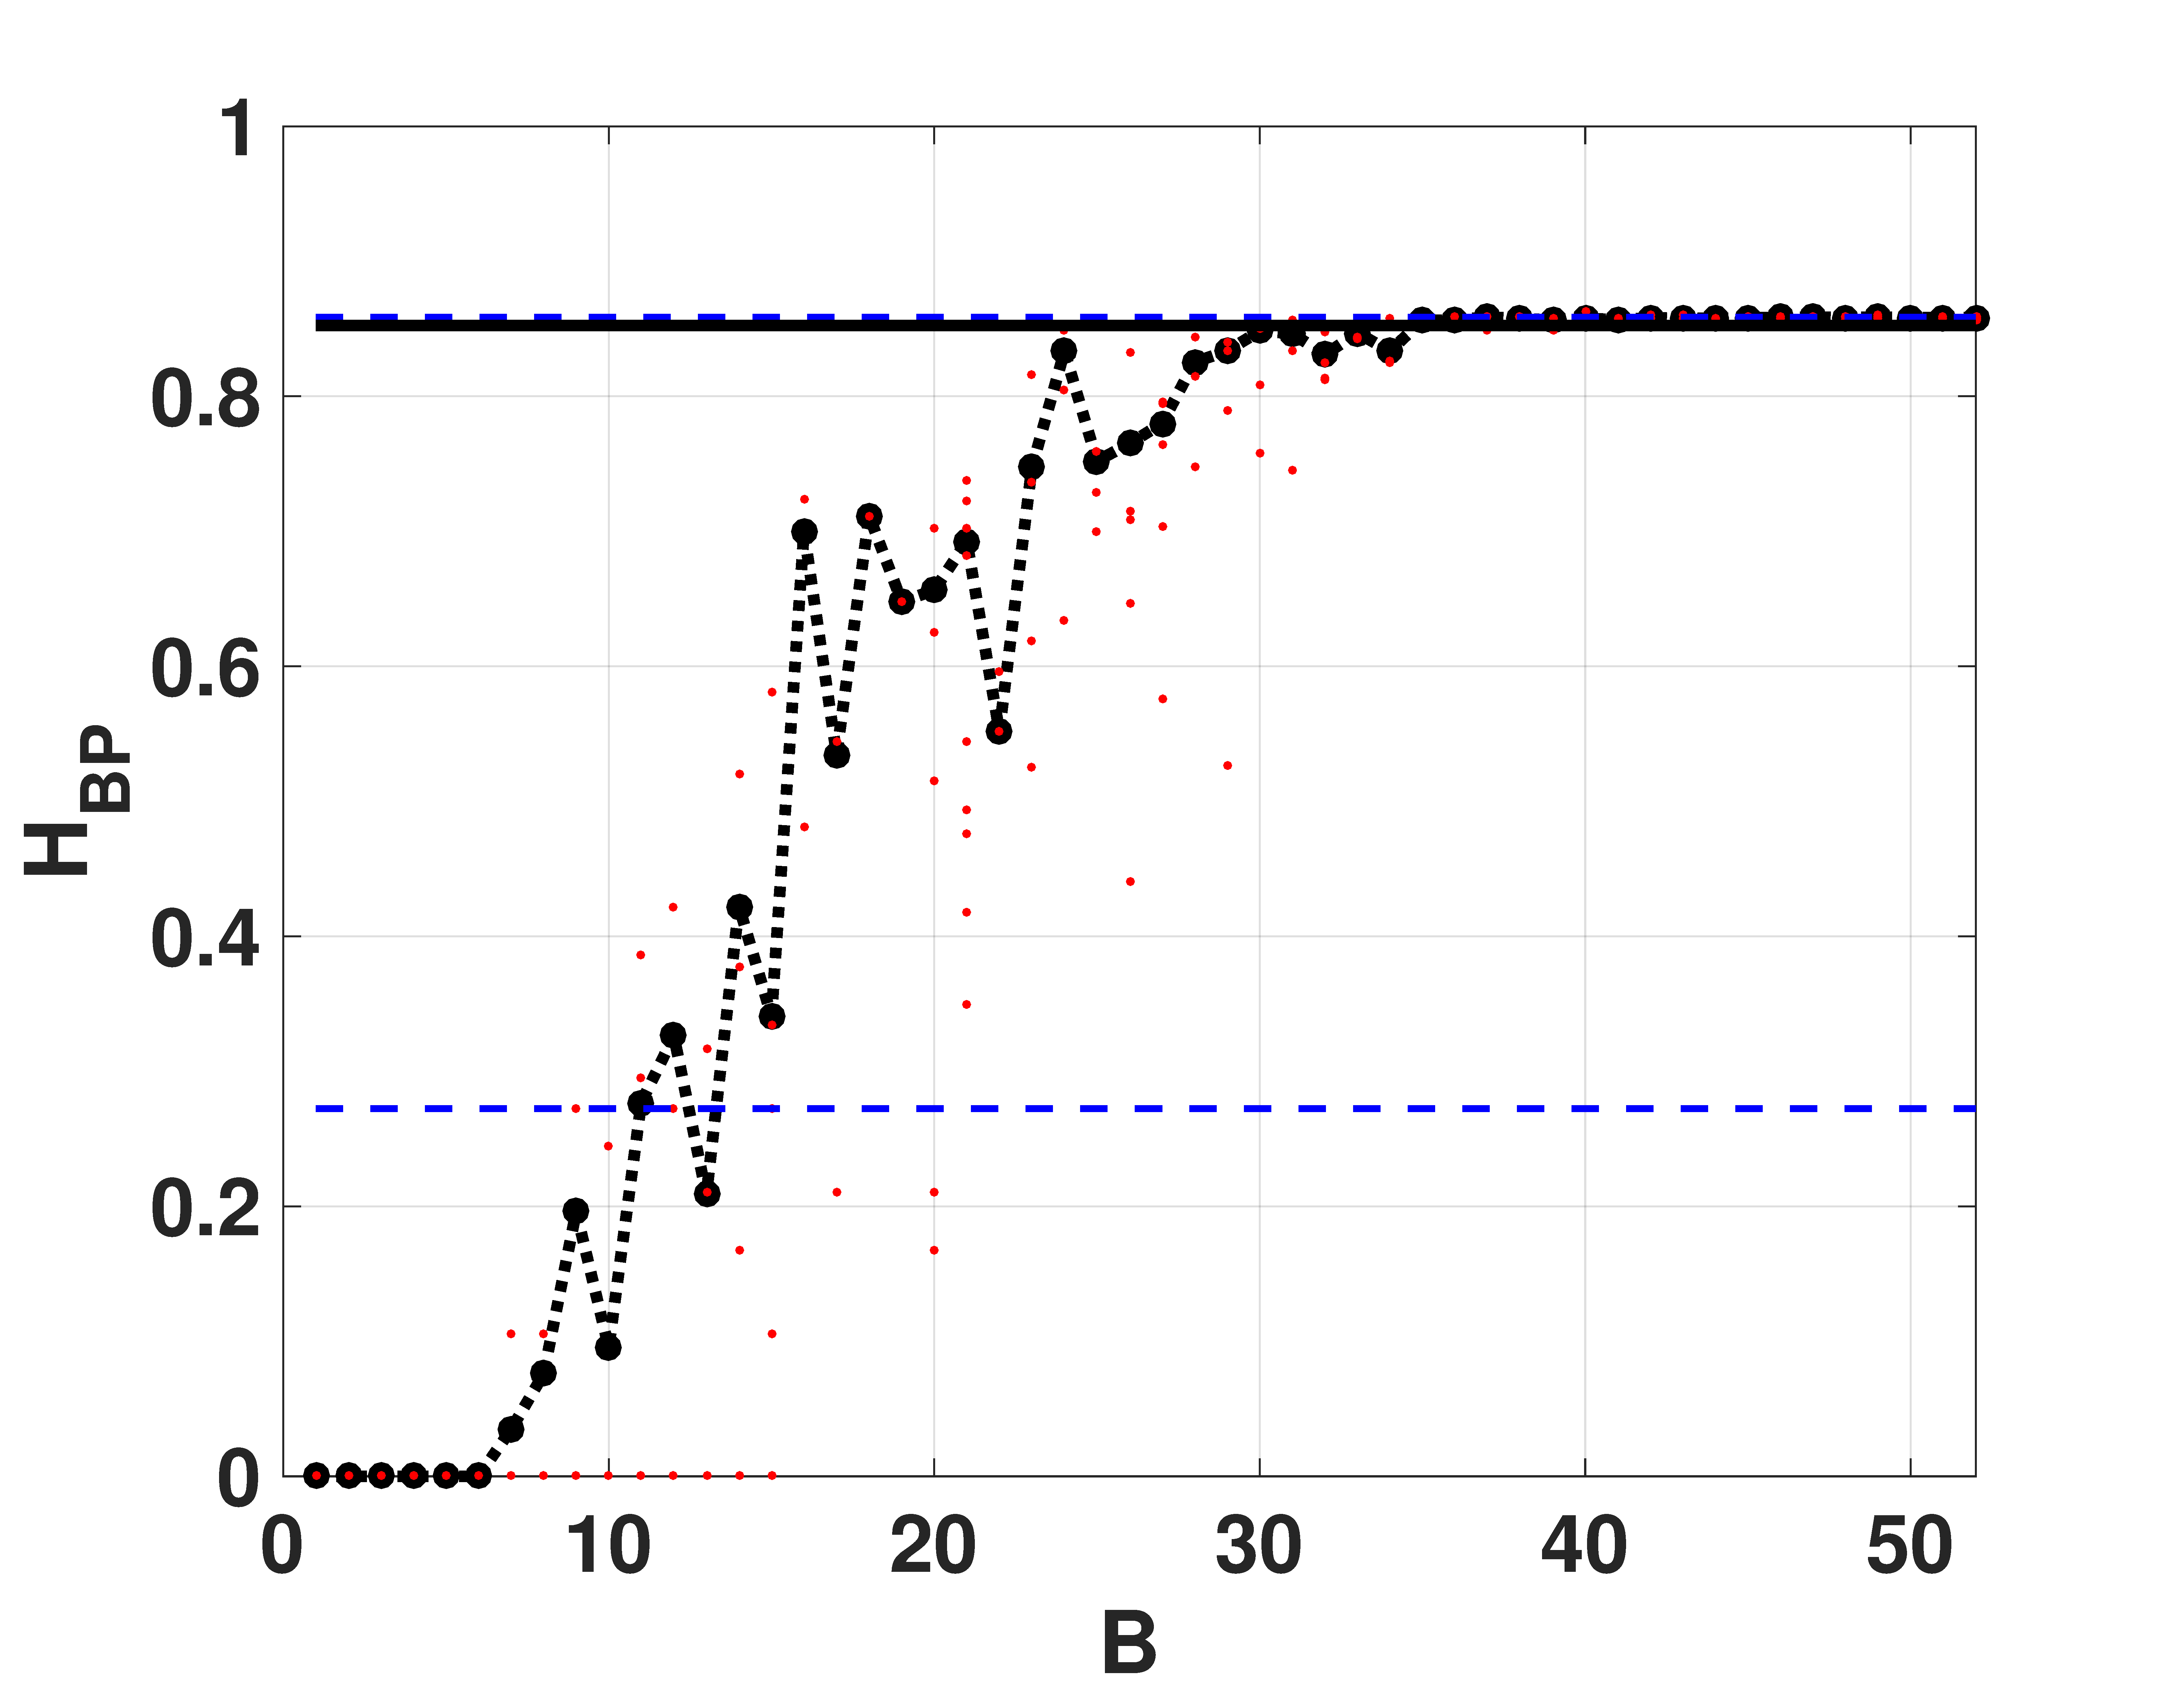
\includegraphics[width=\textwidth]{Hbp_Even}
		\caption{$H_{BP}$ vs. $B$}
		\label{fig:Hbp_Even}
	\end{subfigure}
	\begin{subfigure}[b]{0.49\textwidth}
		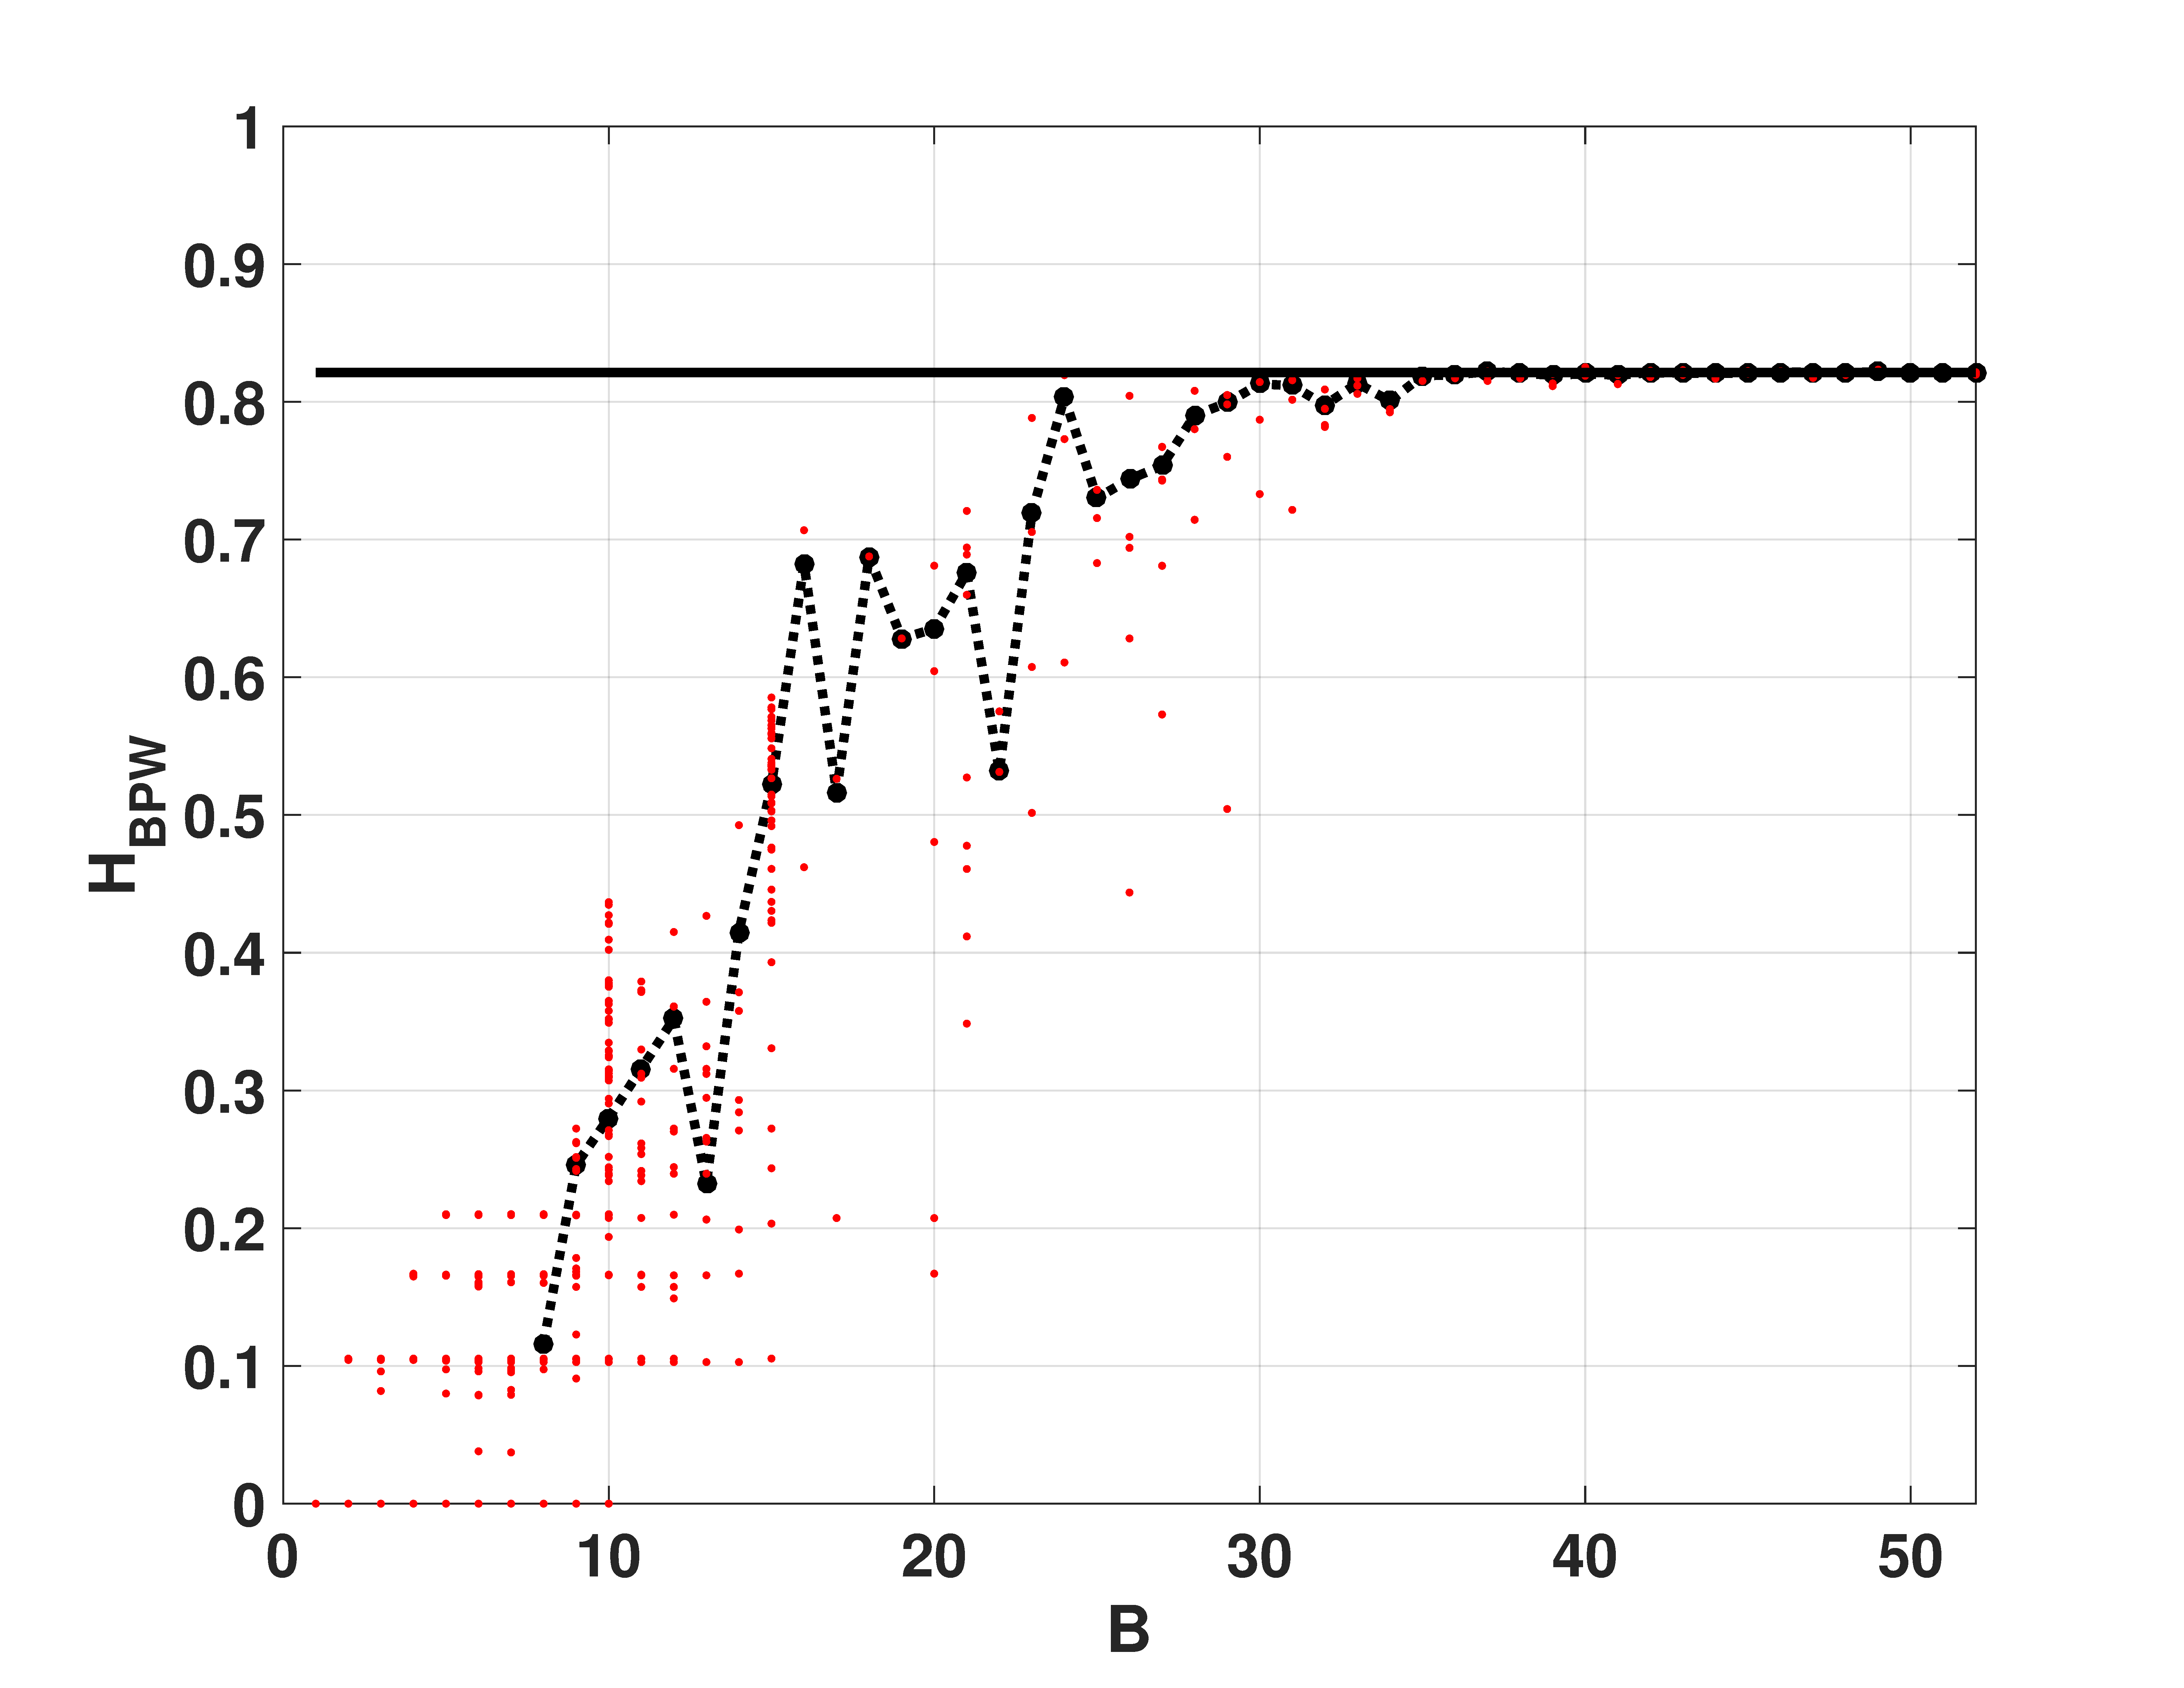
\includegraphics[width=\textwidth]{Hbpw_Even}
		\caption{$H_{BPW}$ vs. $B$}
		\label{fig:Hbpw_Even}
	\end{subfigure}
	\begin{subfigure}[b]{0.49\textwidth}
		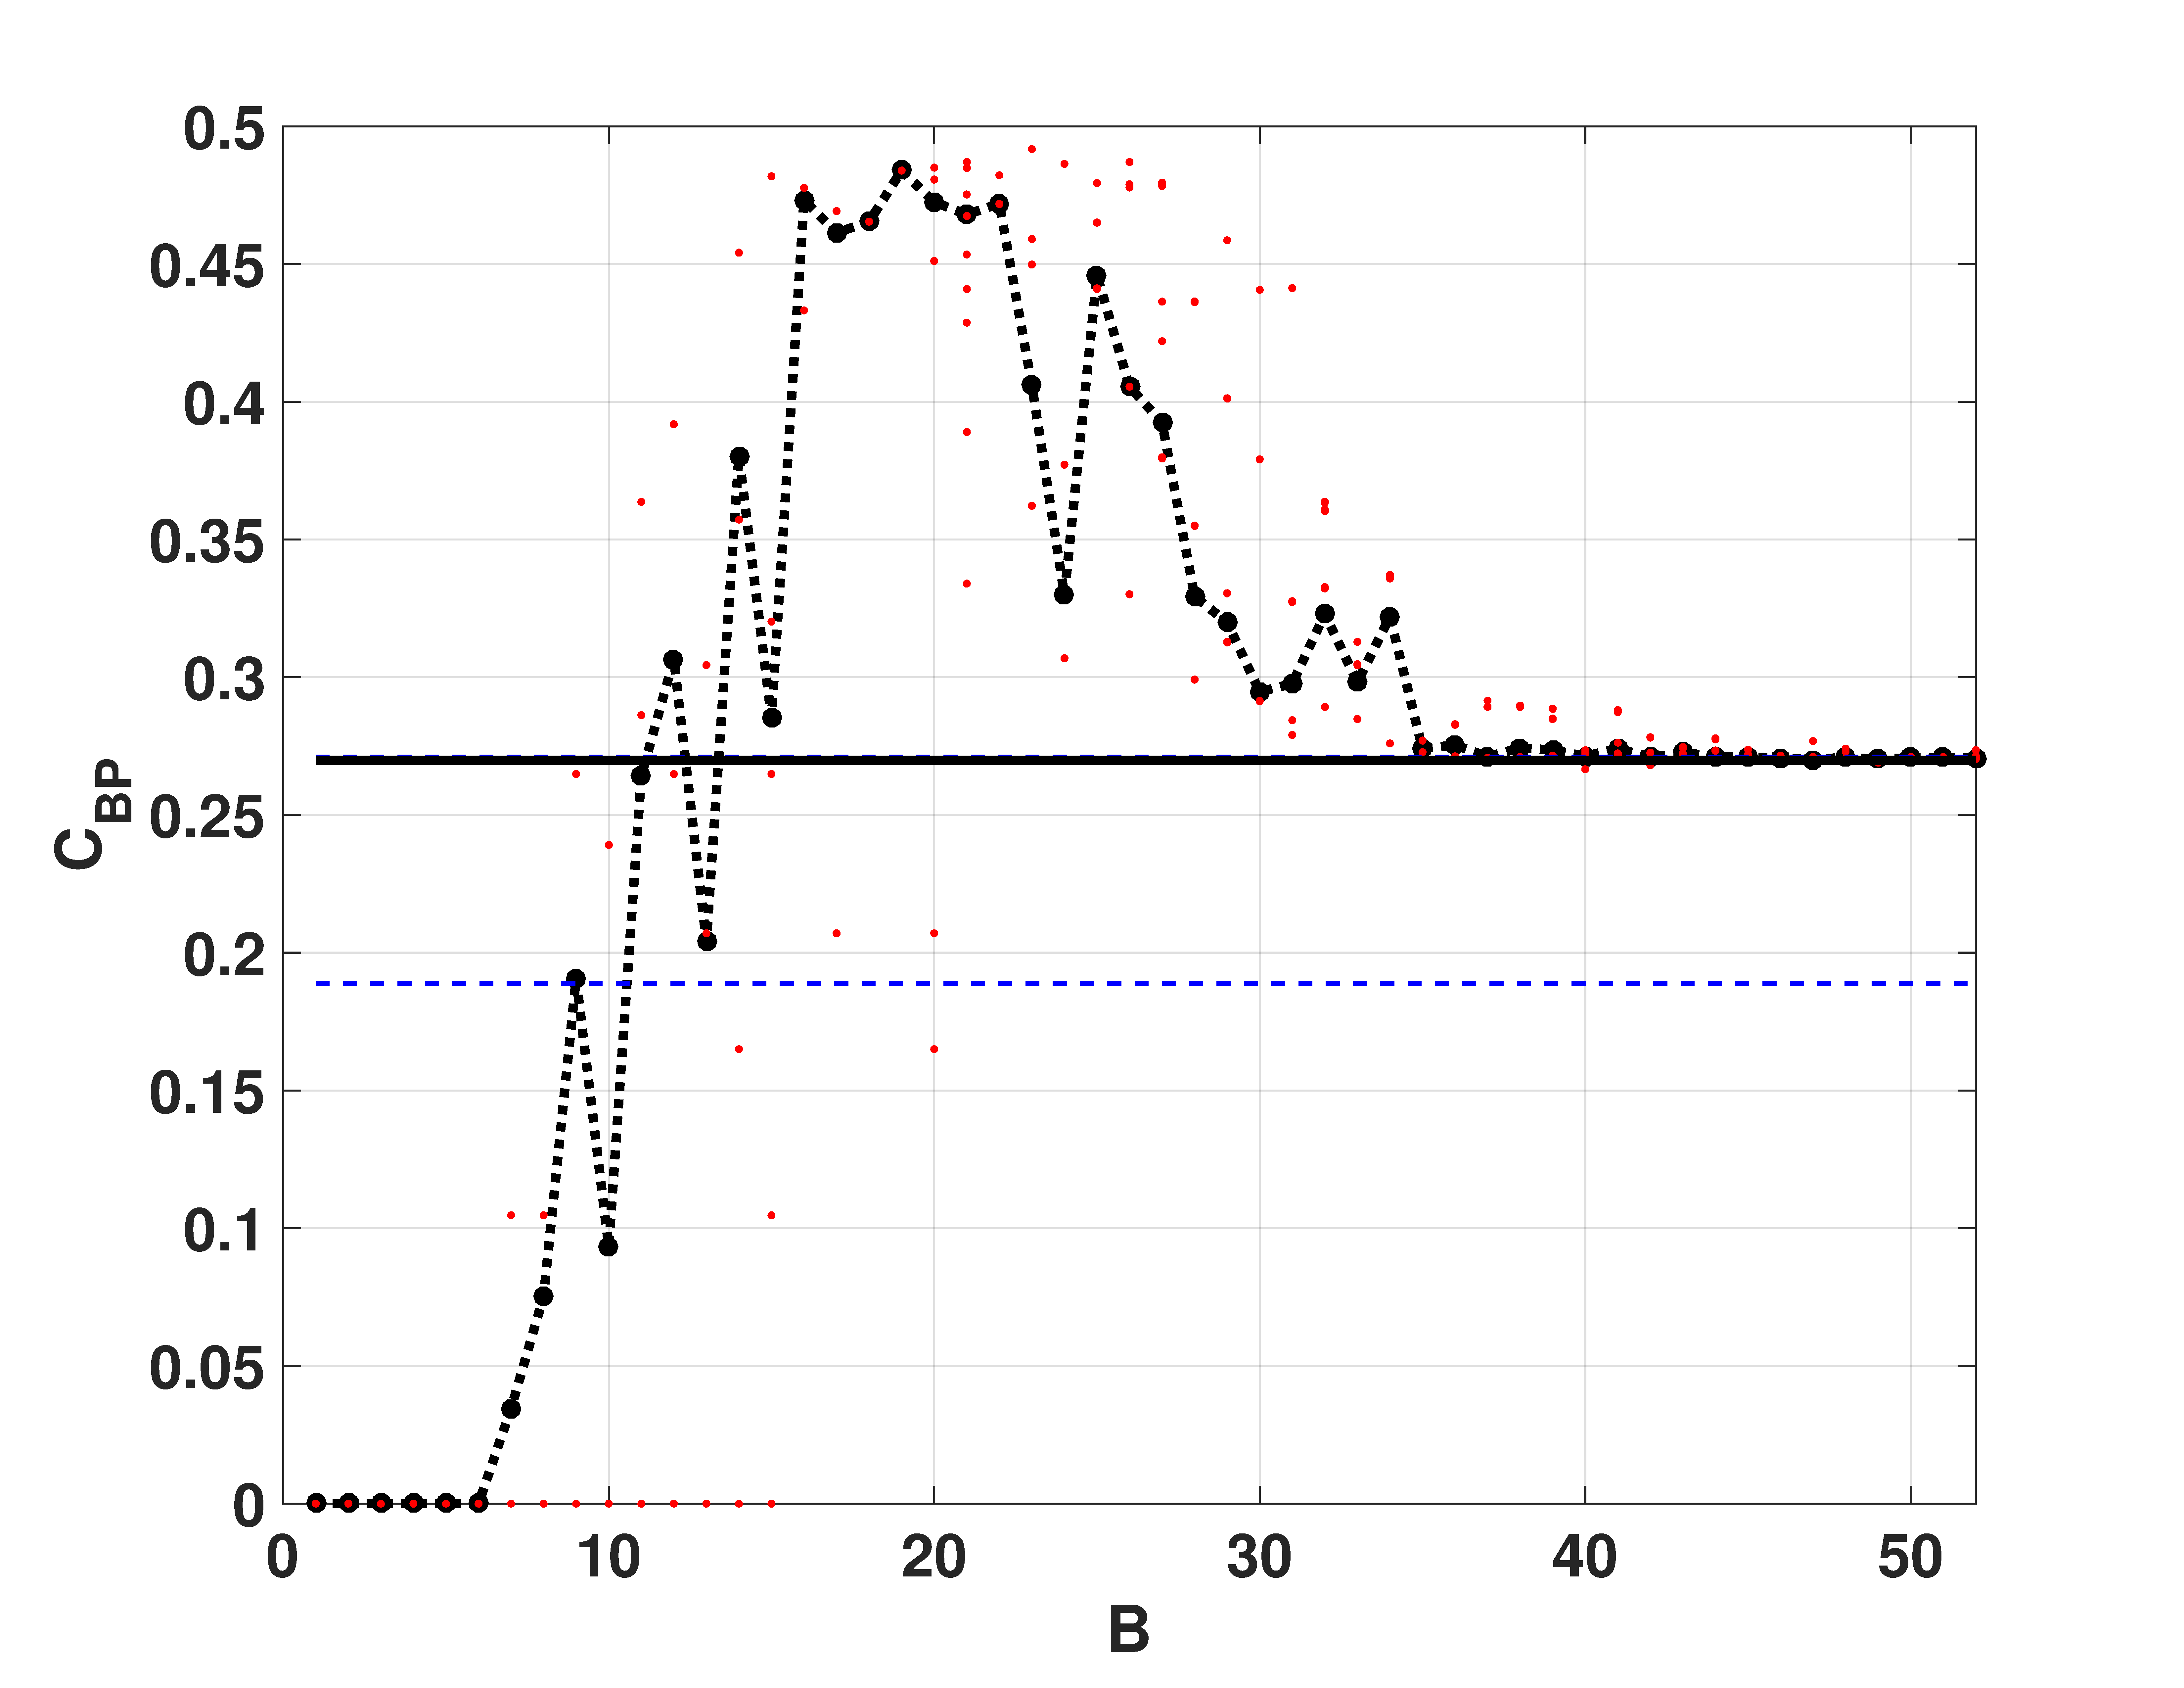
\includegraphics[width=\textwidth]{Cbp_Even}
		\caption{$C_{BP}$ vs. $B$}
		\label{fig:Cbp_Even}
	\end{subfigure}
	\begin{subfigure}[b]{0.49\textwidth}
		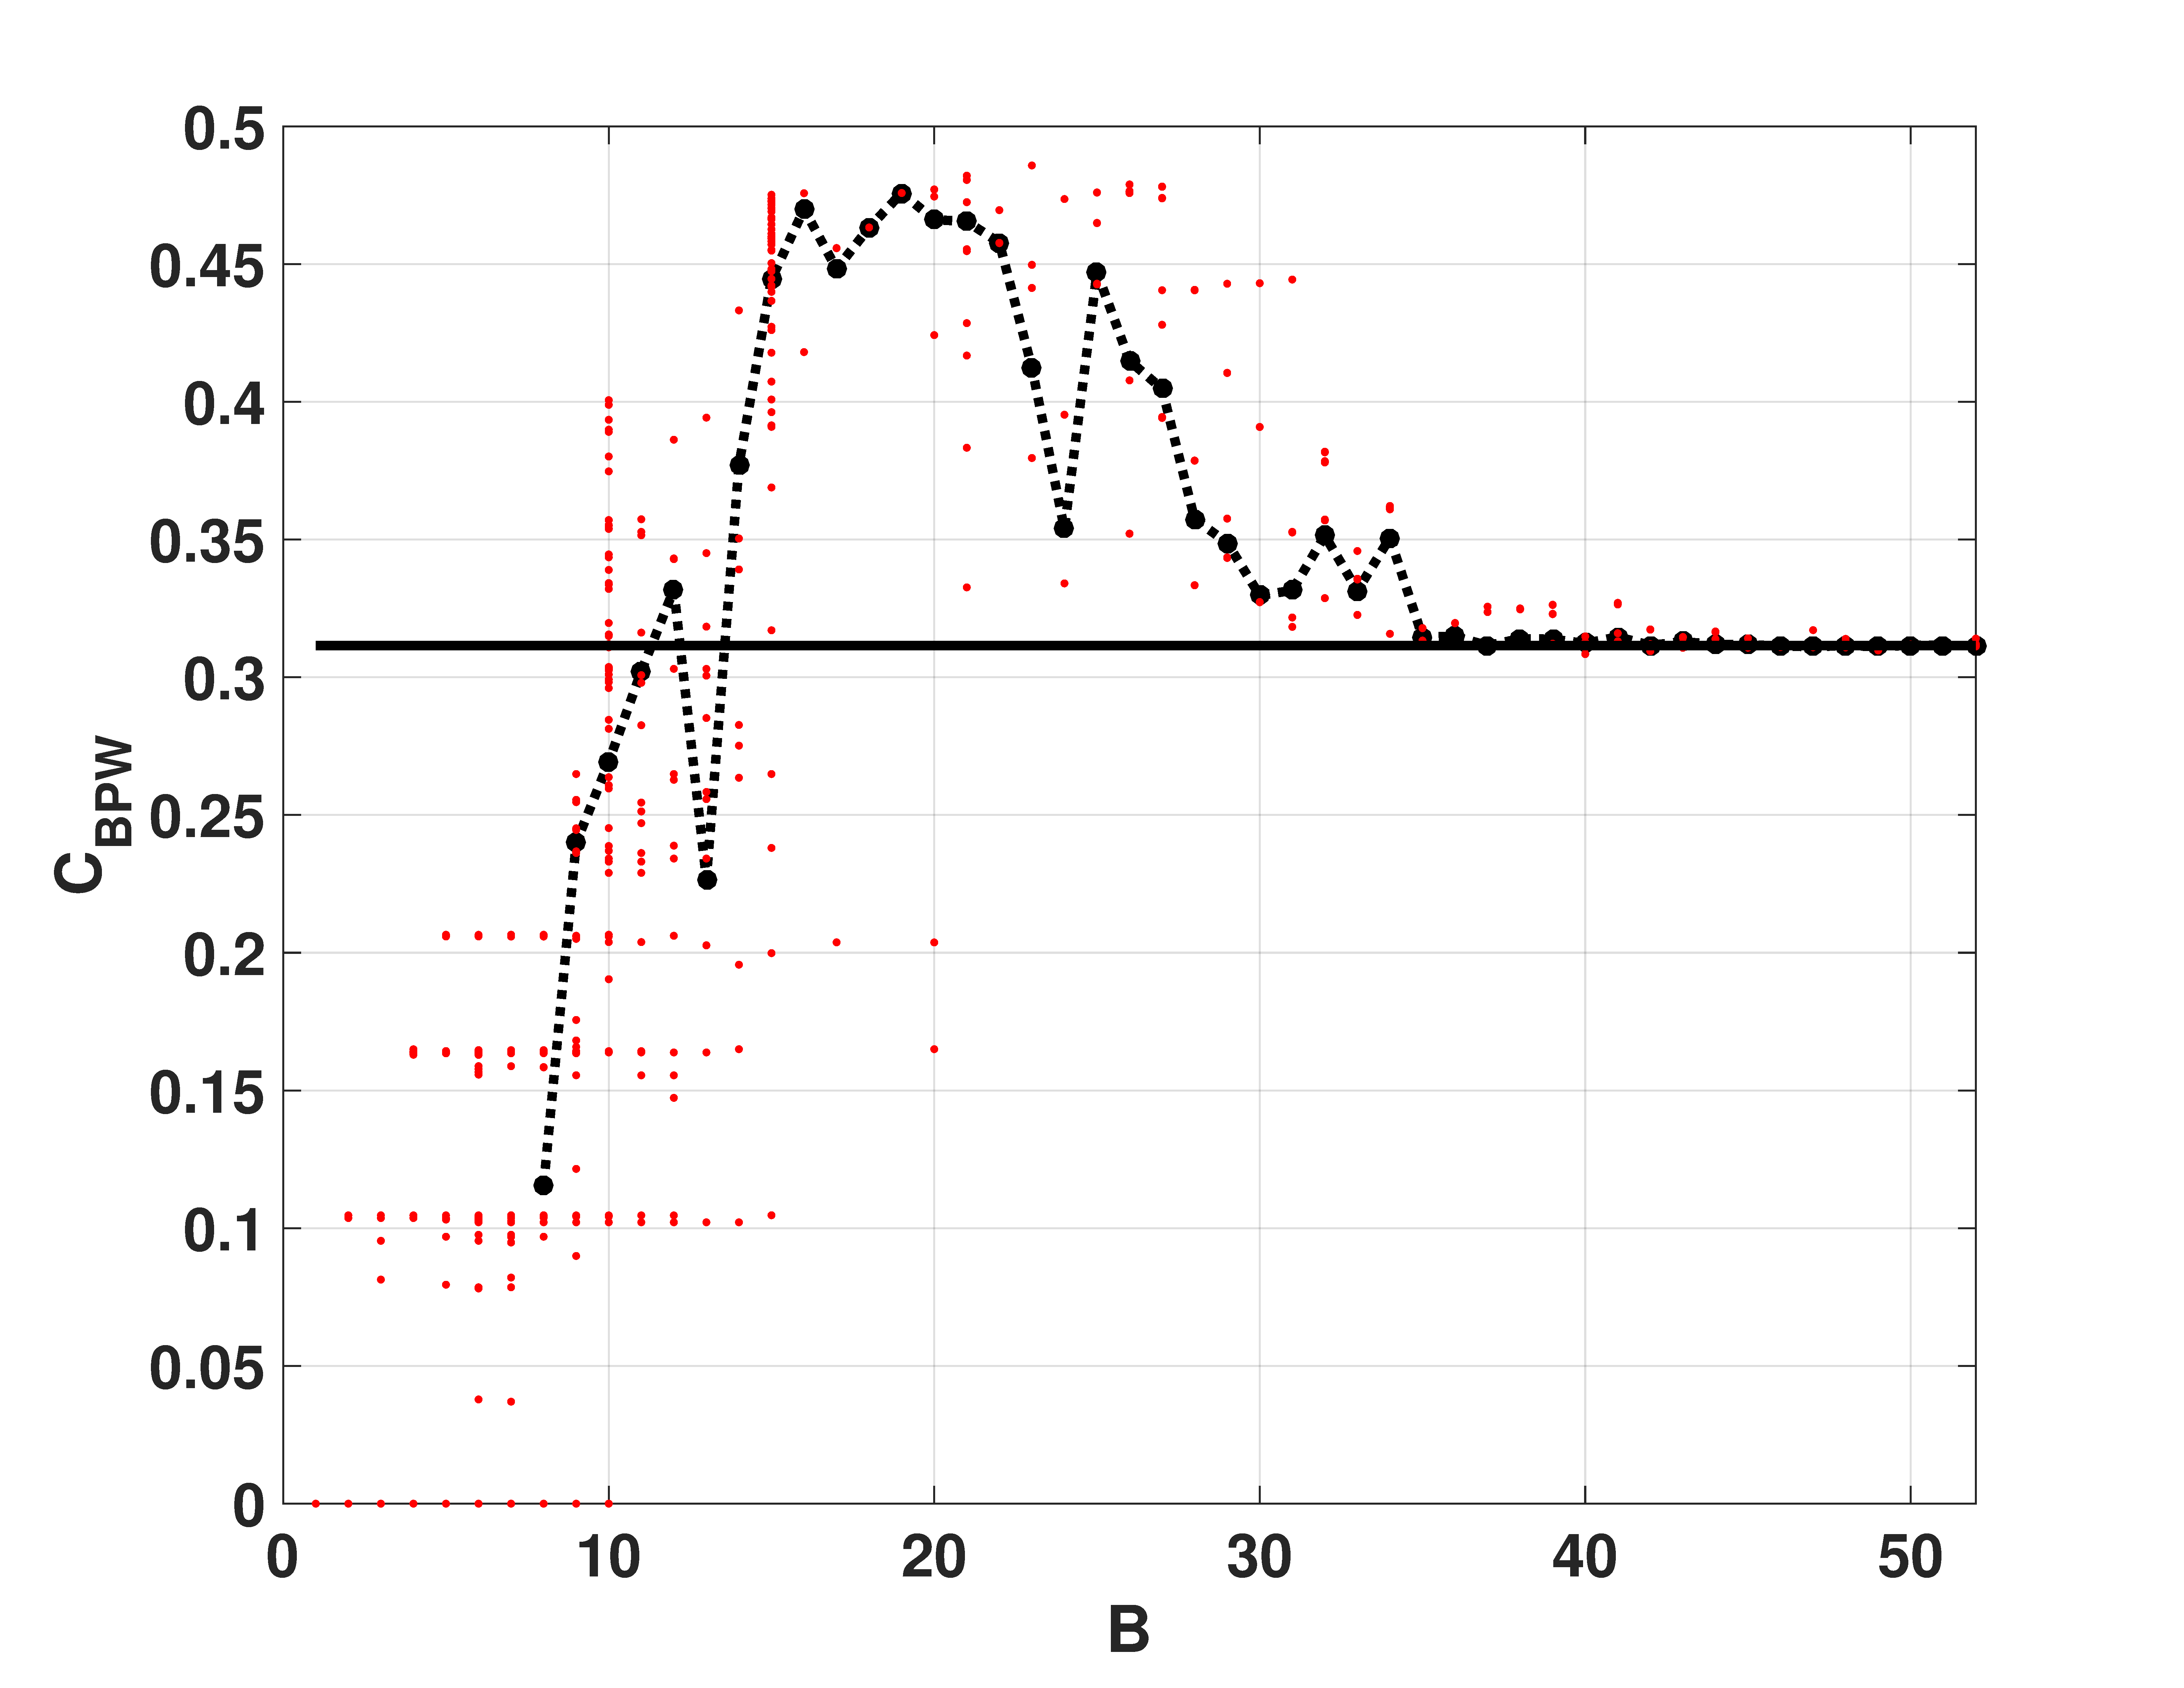
\includegraphics[width=\textwidth]{Cbpw_Even}
		\caption{$C_{BPW}$ vs. $B$}
		\label{fig:Cbpw_Even}
	\end{subfigure}
	\begin{subfigure}[b]{0.49\textwidth}
		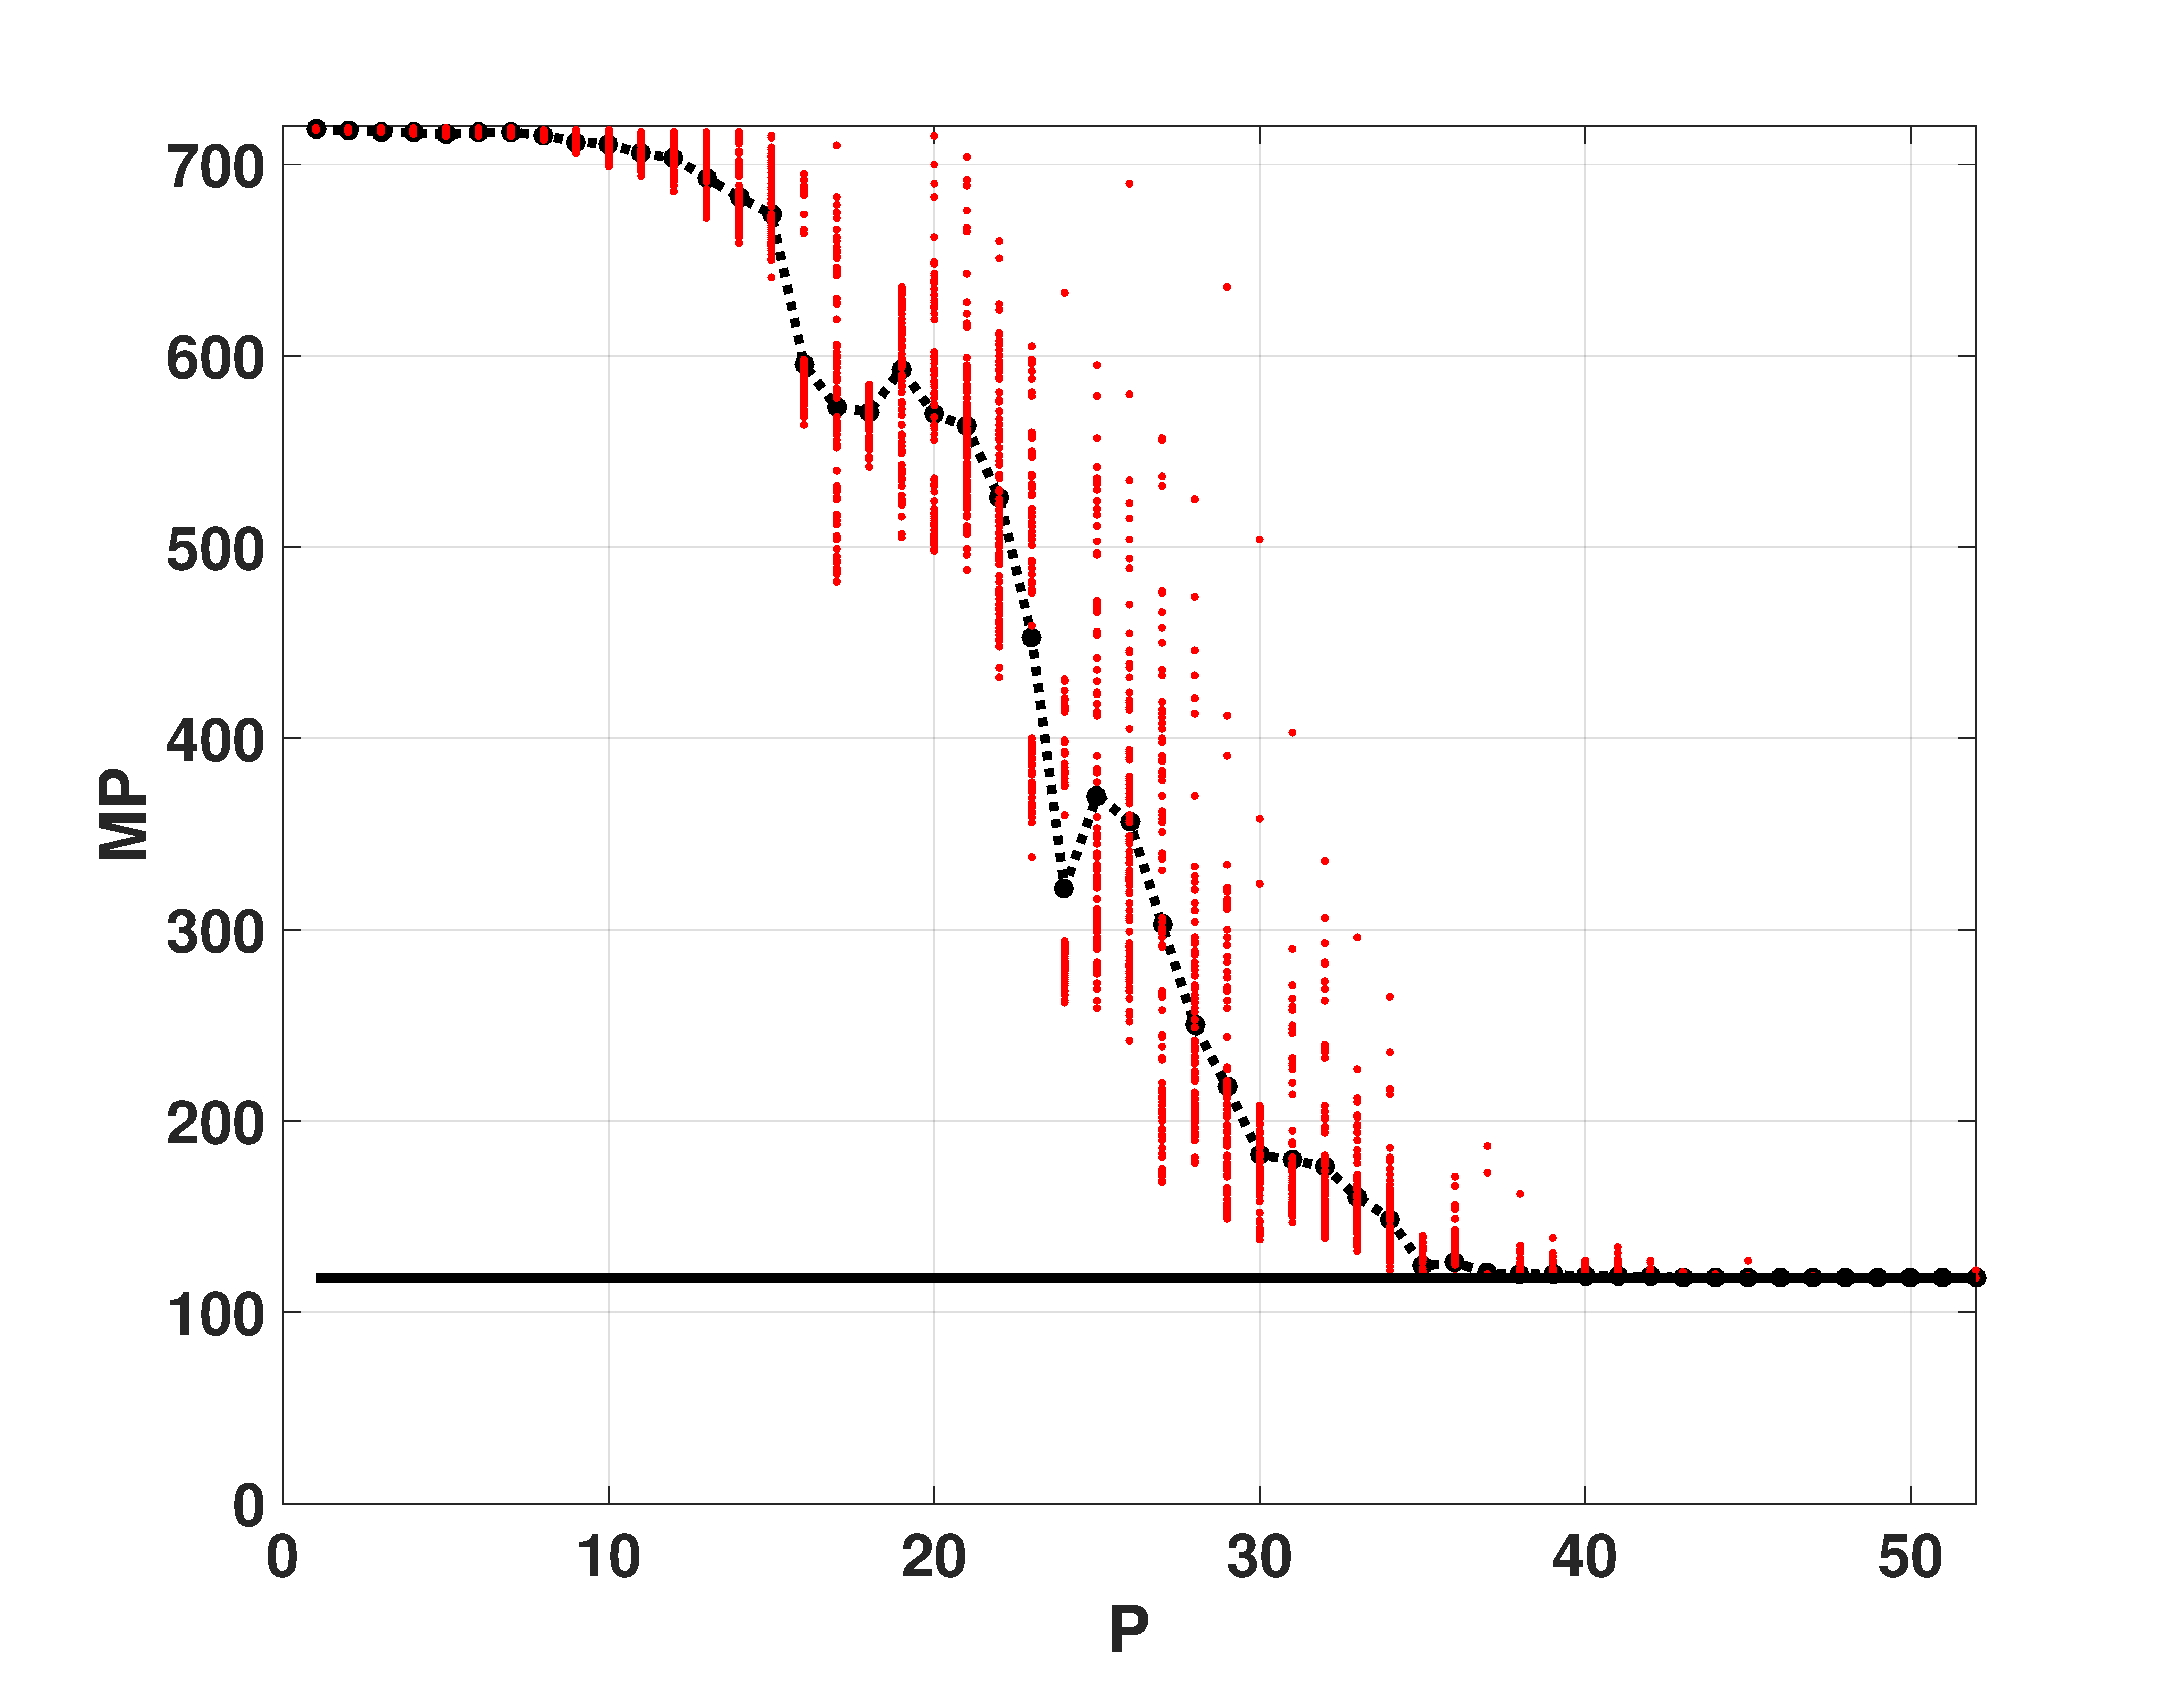
\includegraphics[width=\textwidth]{MP_Even}
		\caption{MP vs. $B$}
		\label{fig:MP_Even}
	\end{subfigure}
	\caption{Statistical properties of EVEN map.}
	\label{fig:EVEN_QuantiB}
\end{figure}
%
\begin{figure}[H]
	\centering
	\begin{subfigure}[b]{0.49\textwidth}
		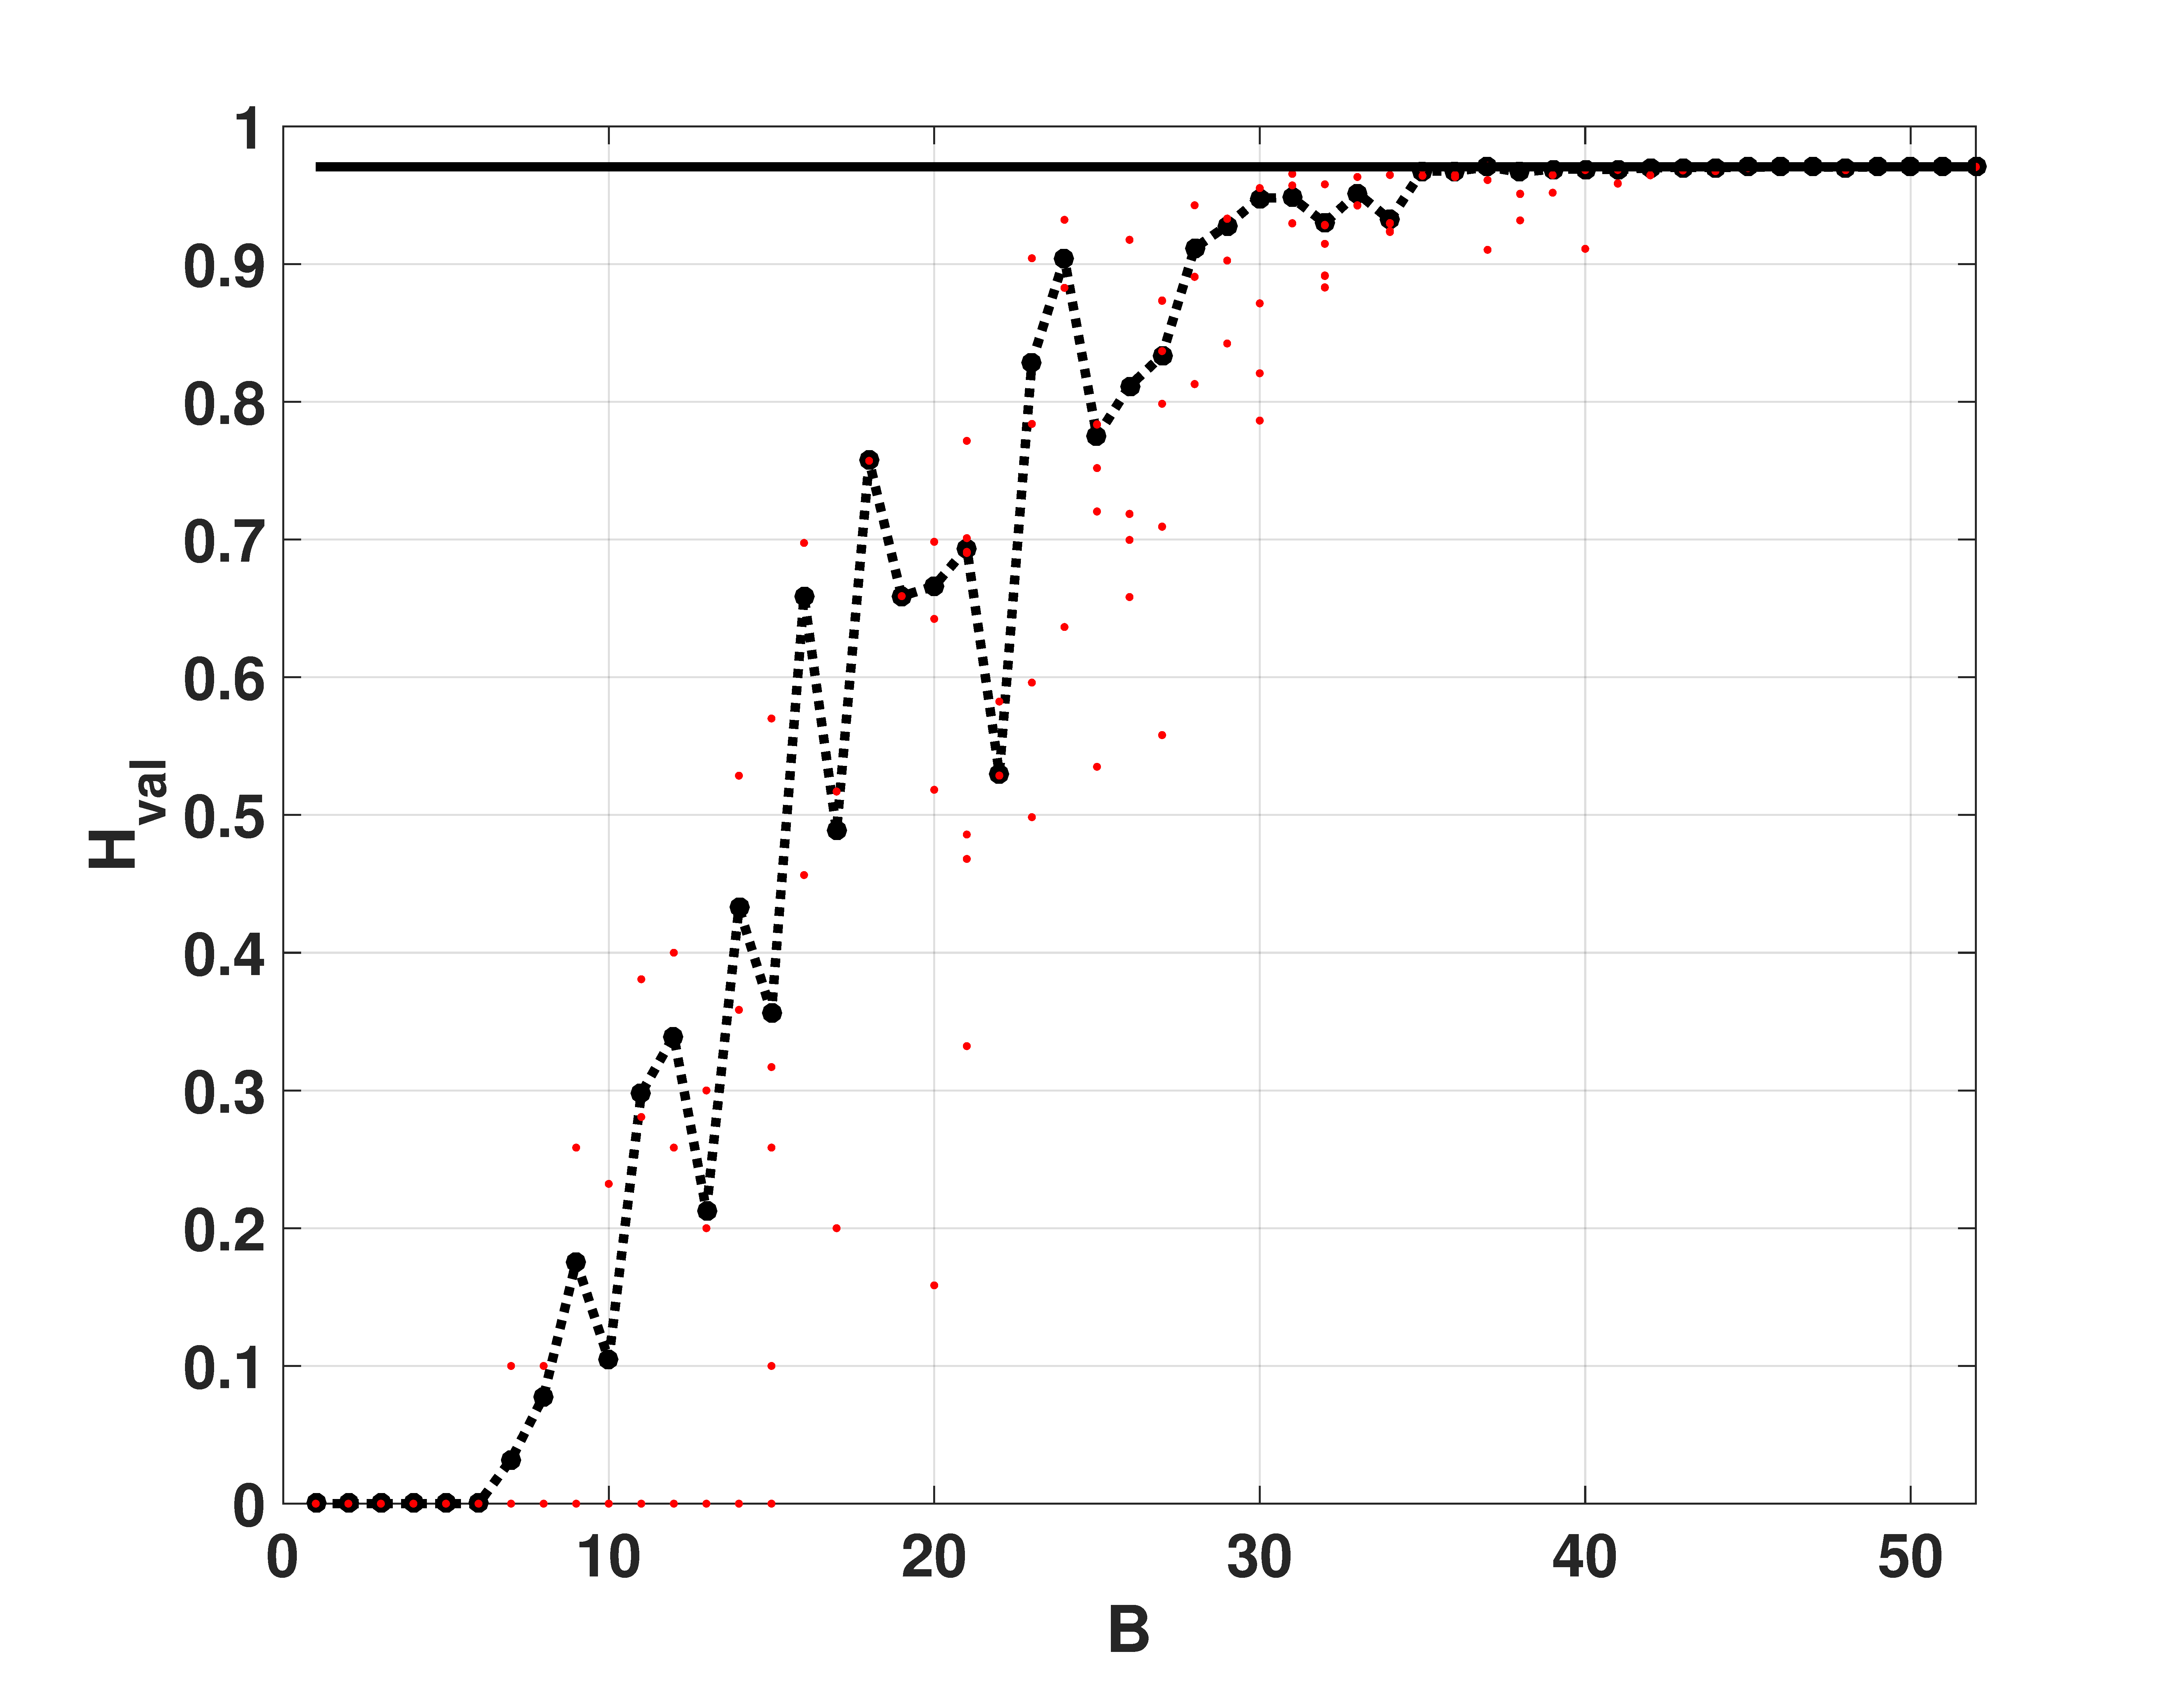
\includegraphics[width=\textwidth]{Hval_Odd}
		\caption{$H_{hist}$ vs. $B$}
		\label{fig:Hval_Odd}
	\end{subfigure}
	\begin{subfigure}[b]{0.49\textwidth}
		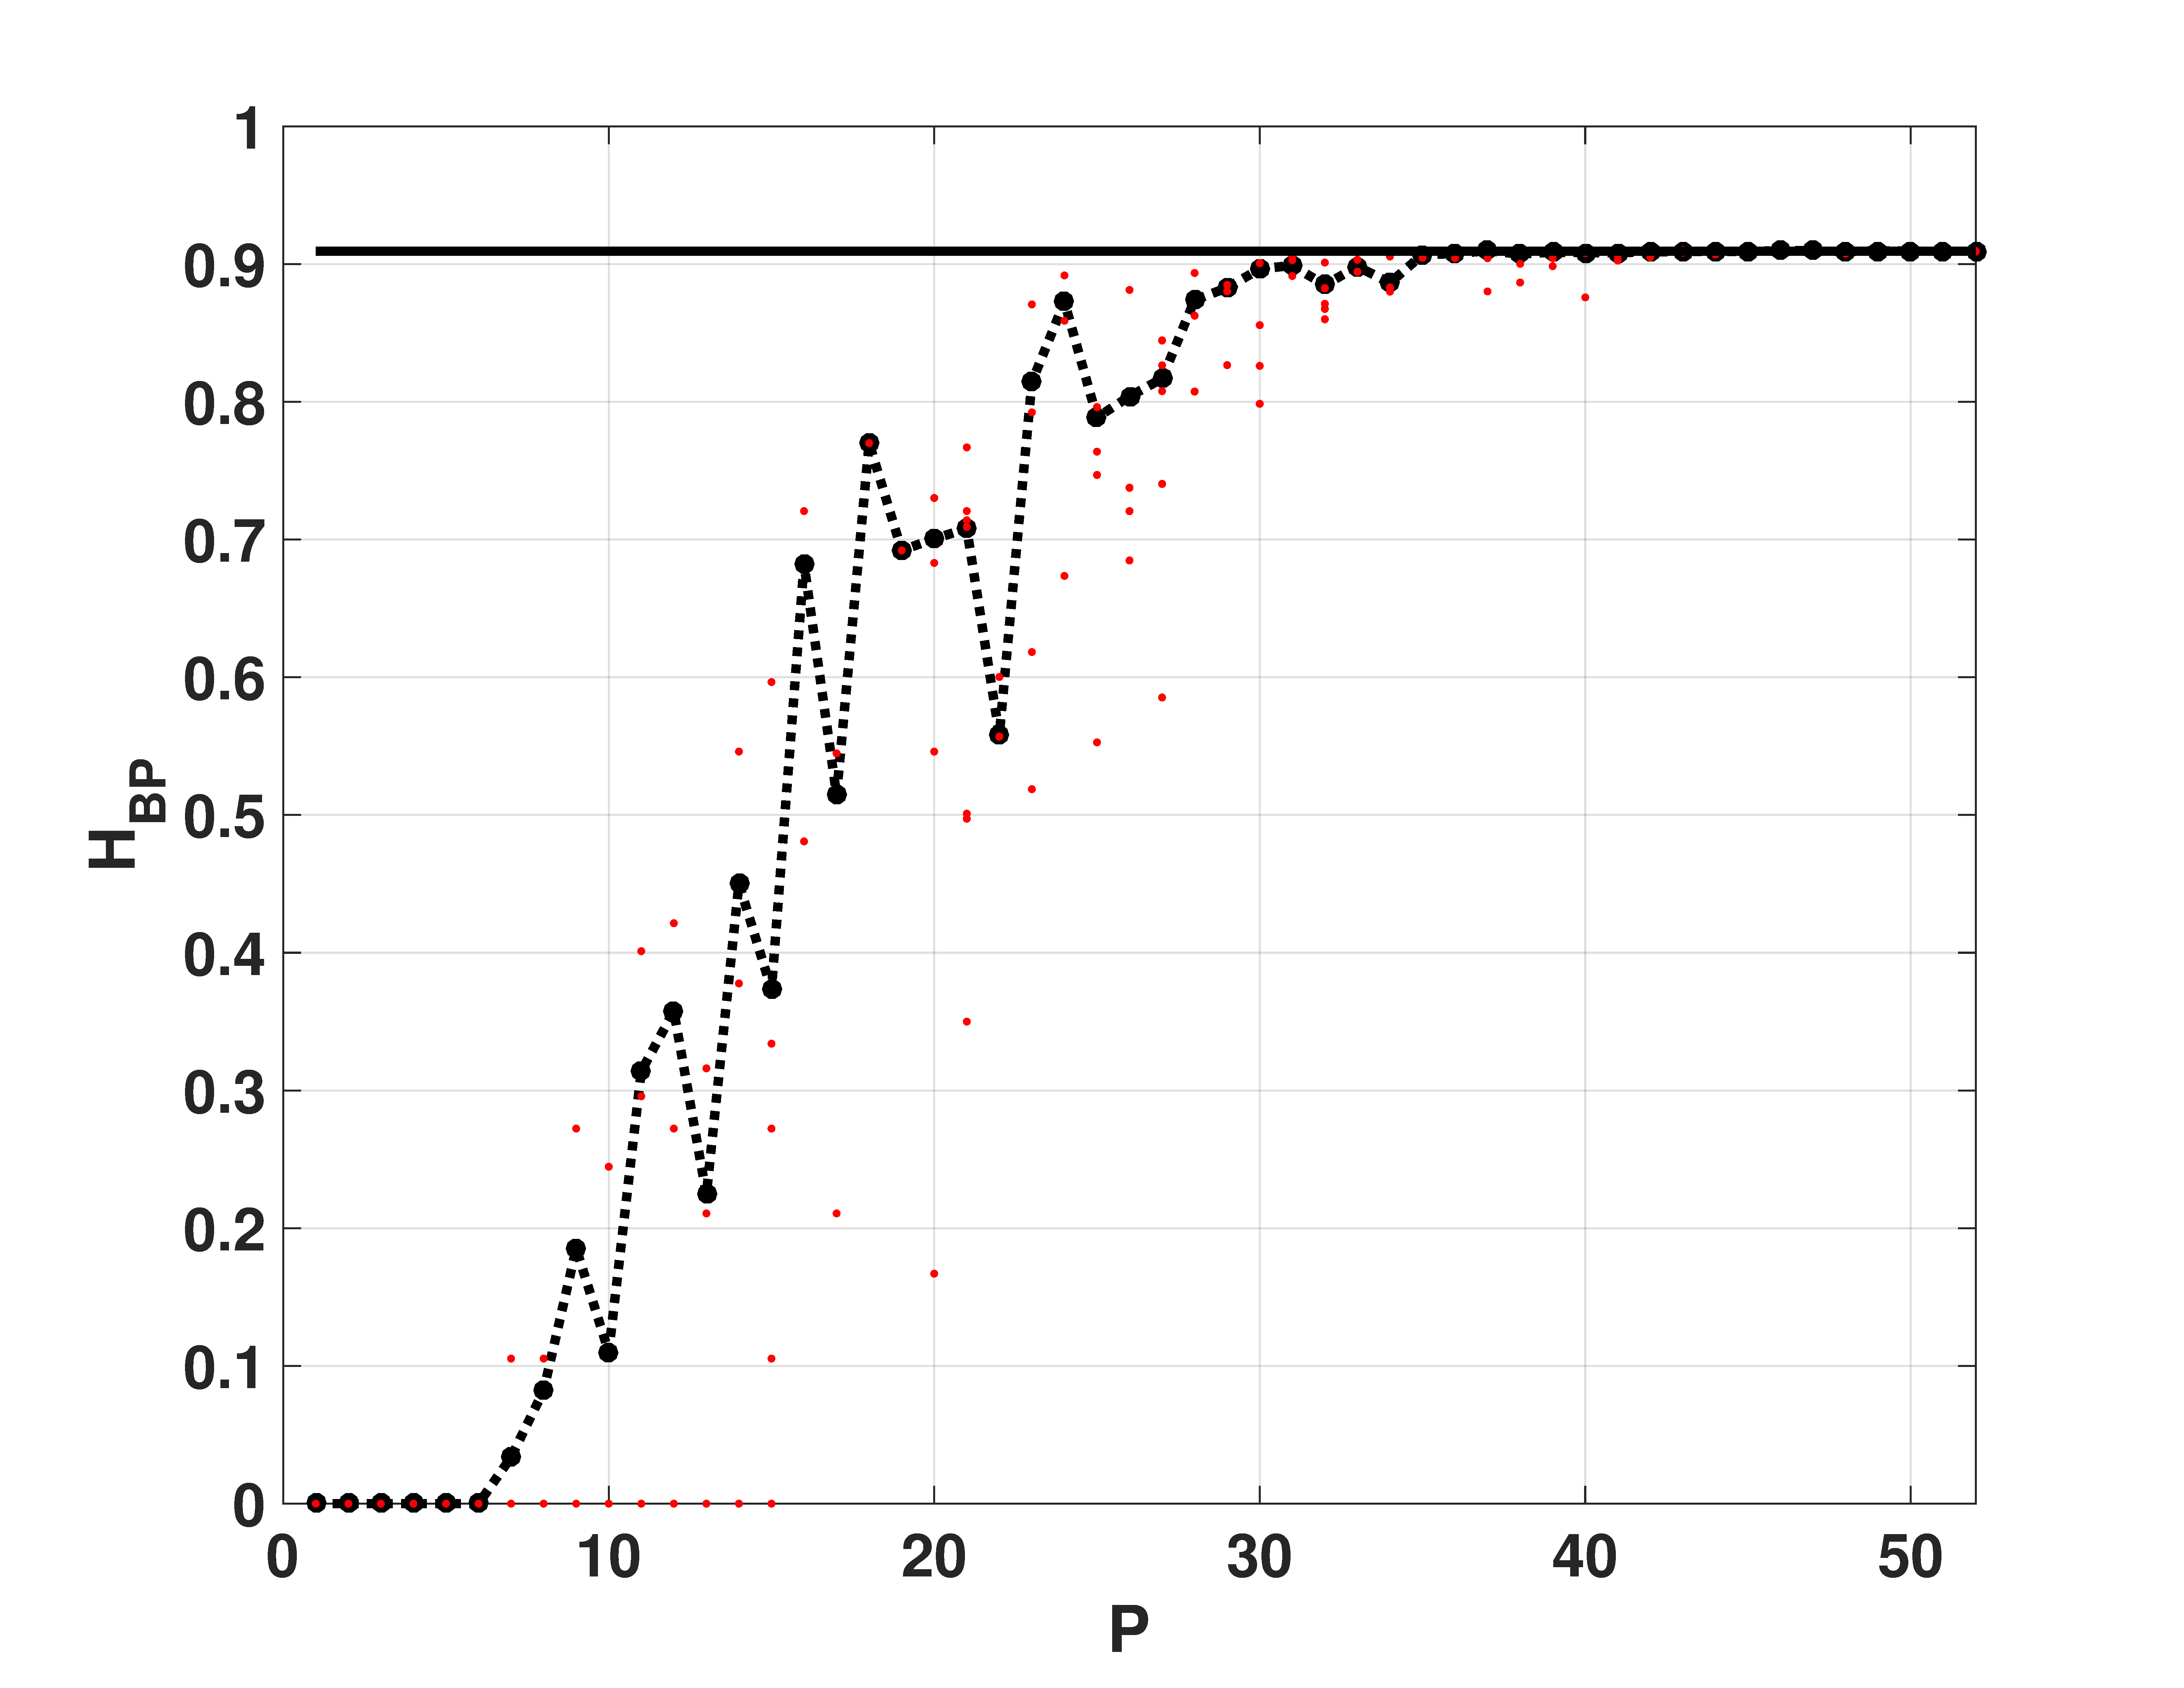
\includegraphics[width=\textwidth]{Hbp_Odd}
		\caption{$H_{BP}$ vs. $B$}
		\label{fig:Hbp_Odd}
	\end{subfigure}
	\begin{subfigure}[b]{0.49\textwidth}
		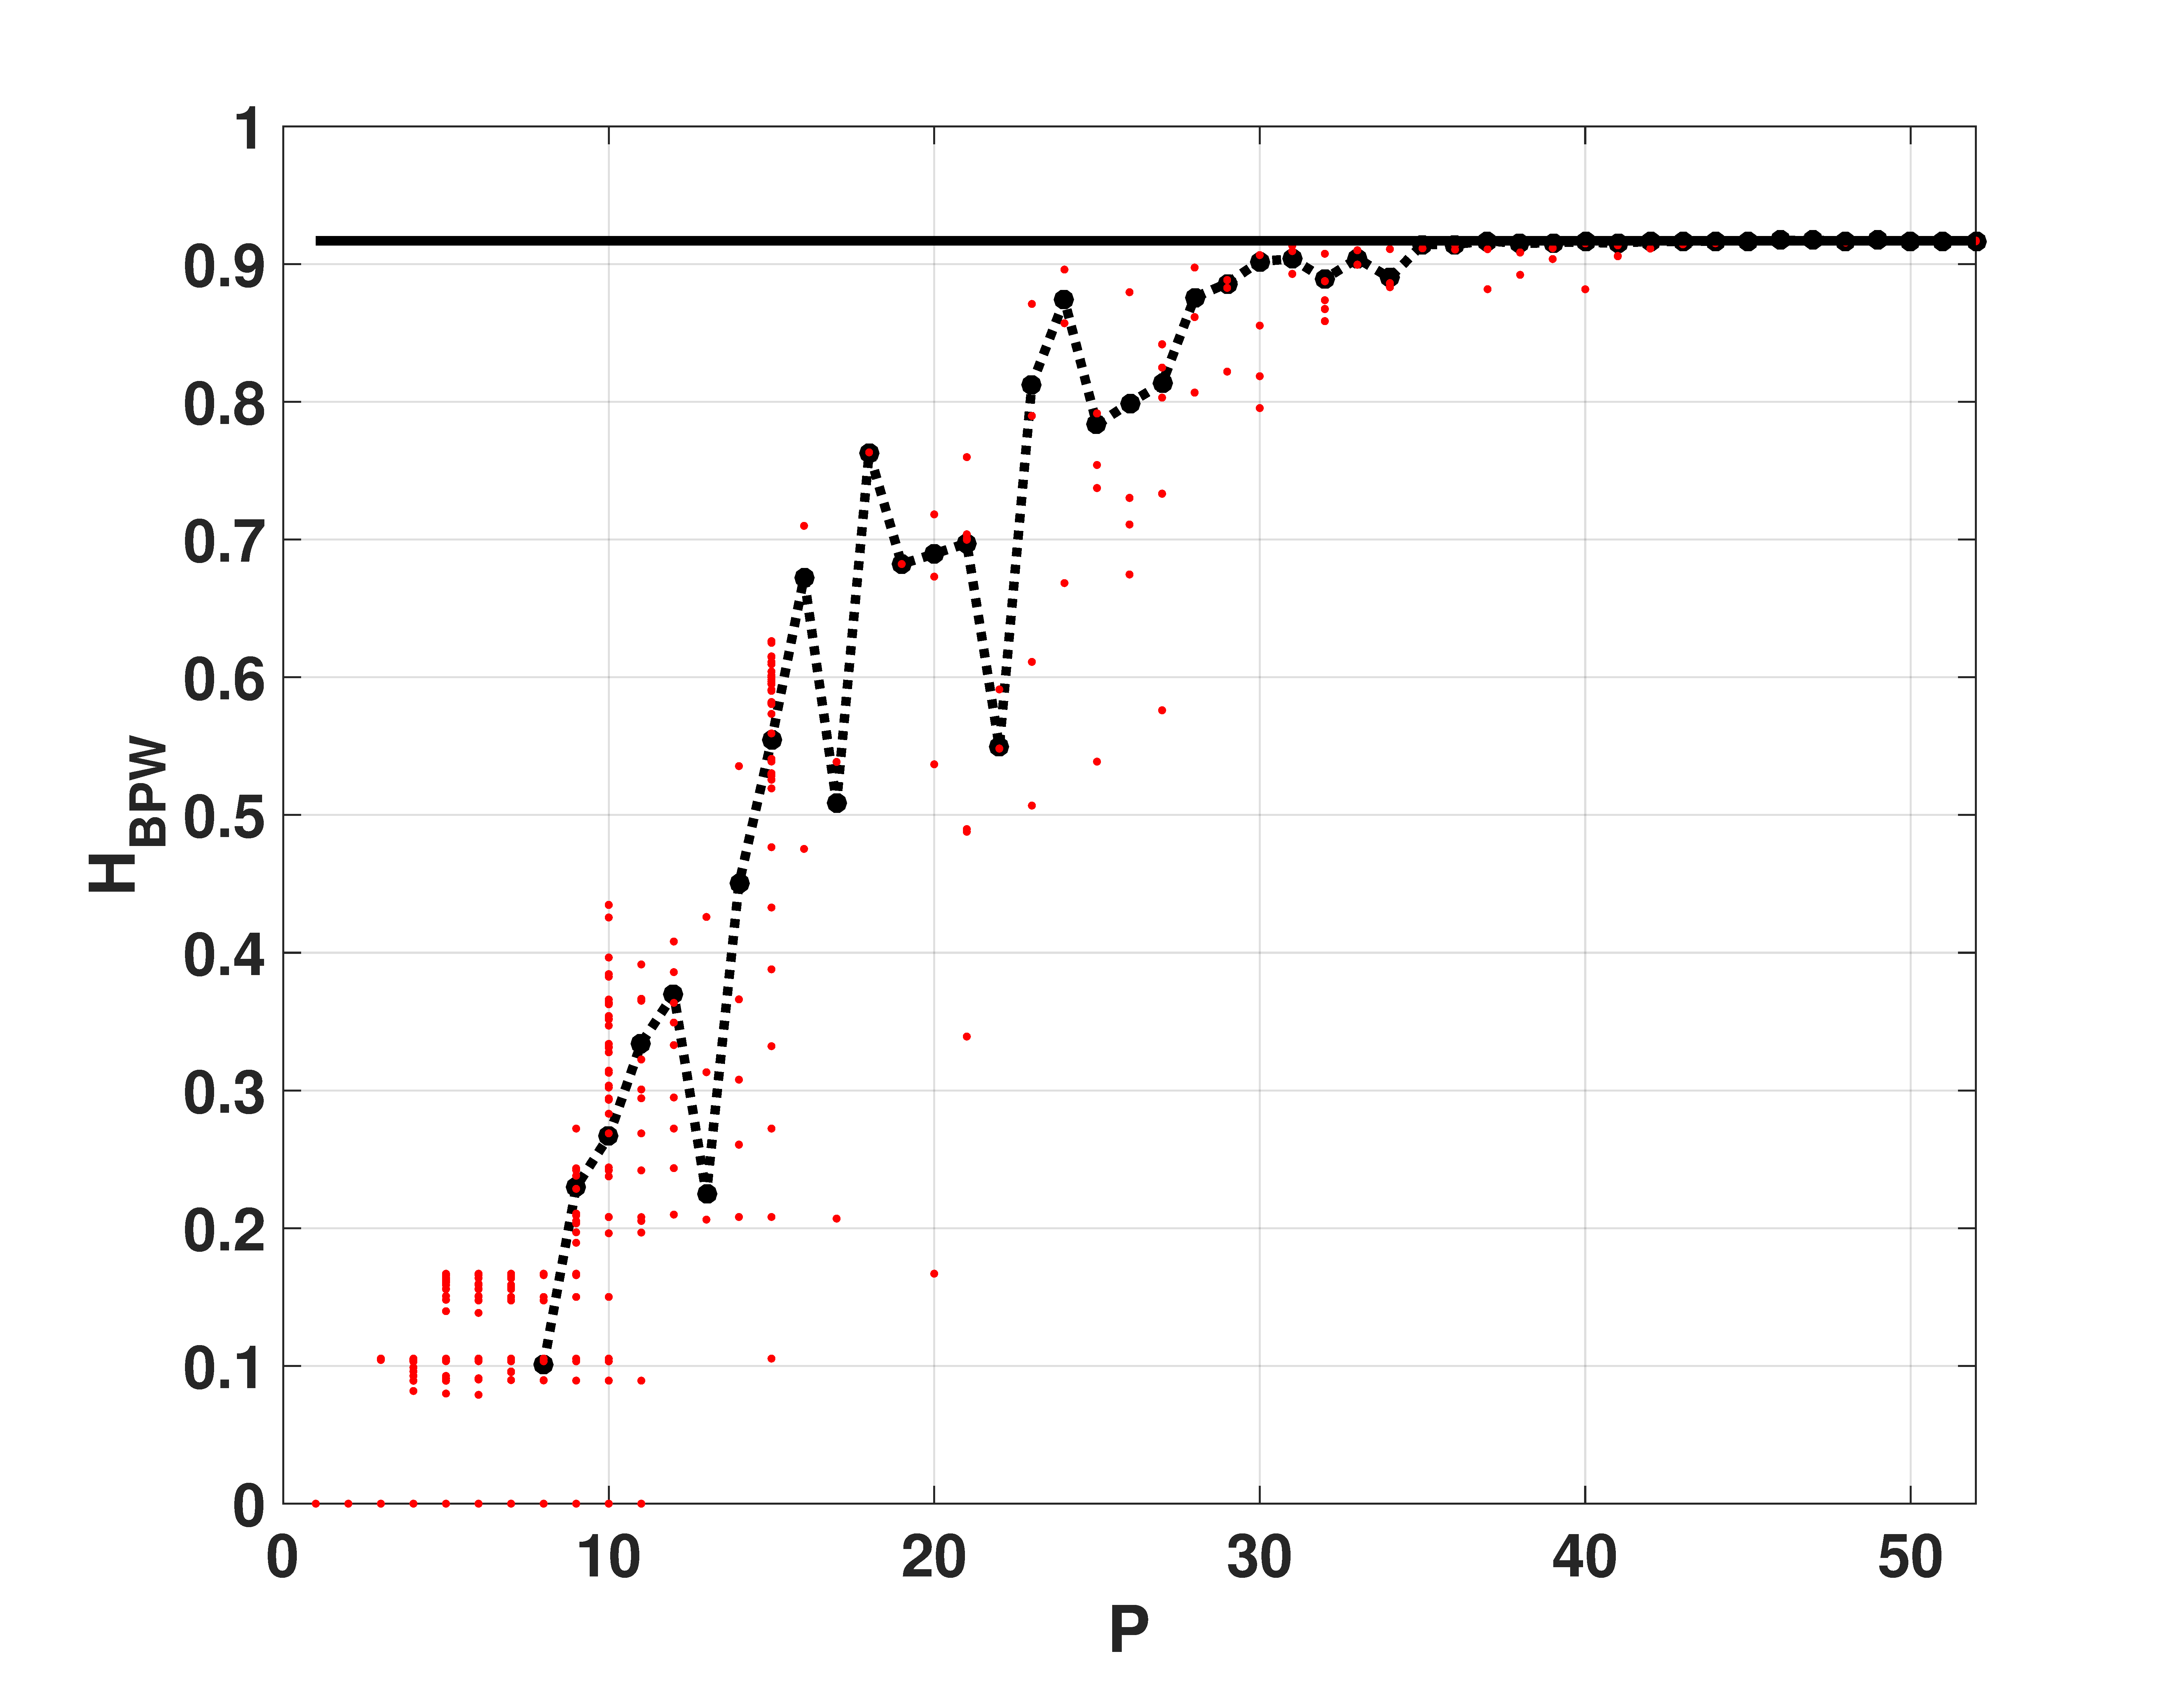
\includegraphics[width=\textwidth]{Hbpw_Odd}
		\caption{$H_{BPW}$ vs. $B$}
		\label{fig:Hbpw_Odd}
	\end{subfigure}
	\begin{subfigure}[b]{0.49\textwidth}
		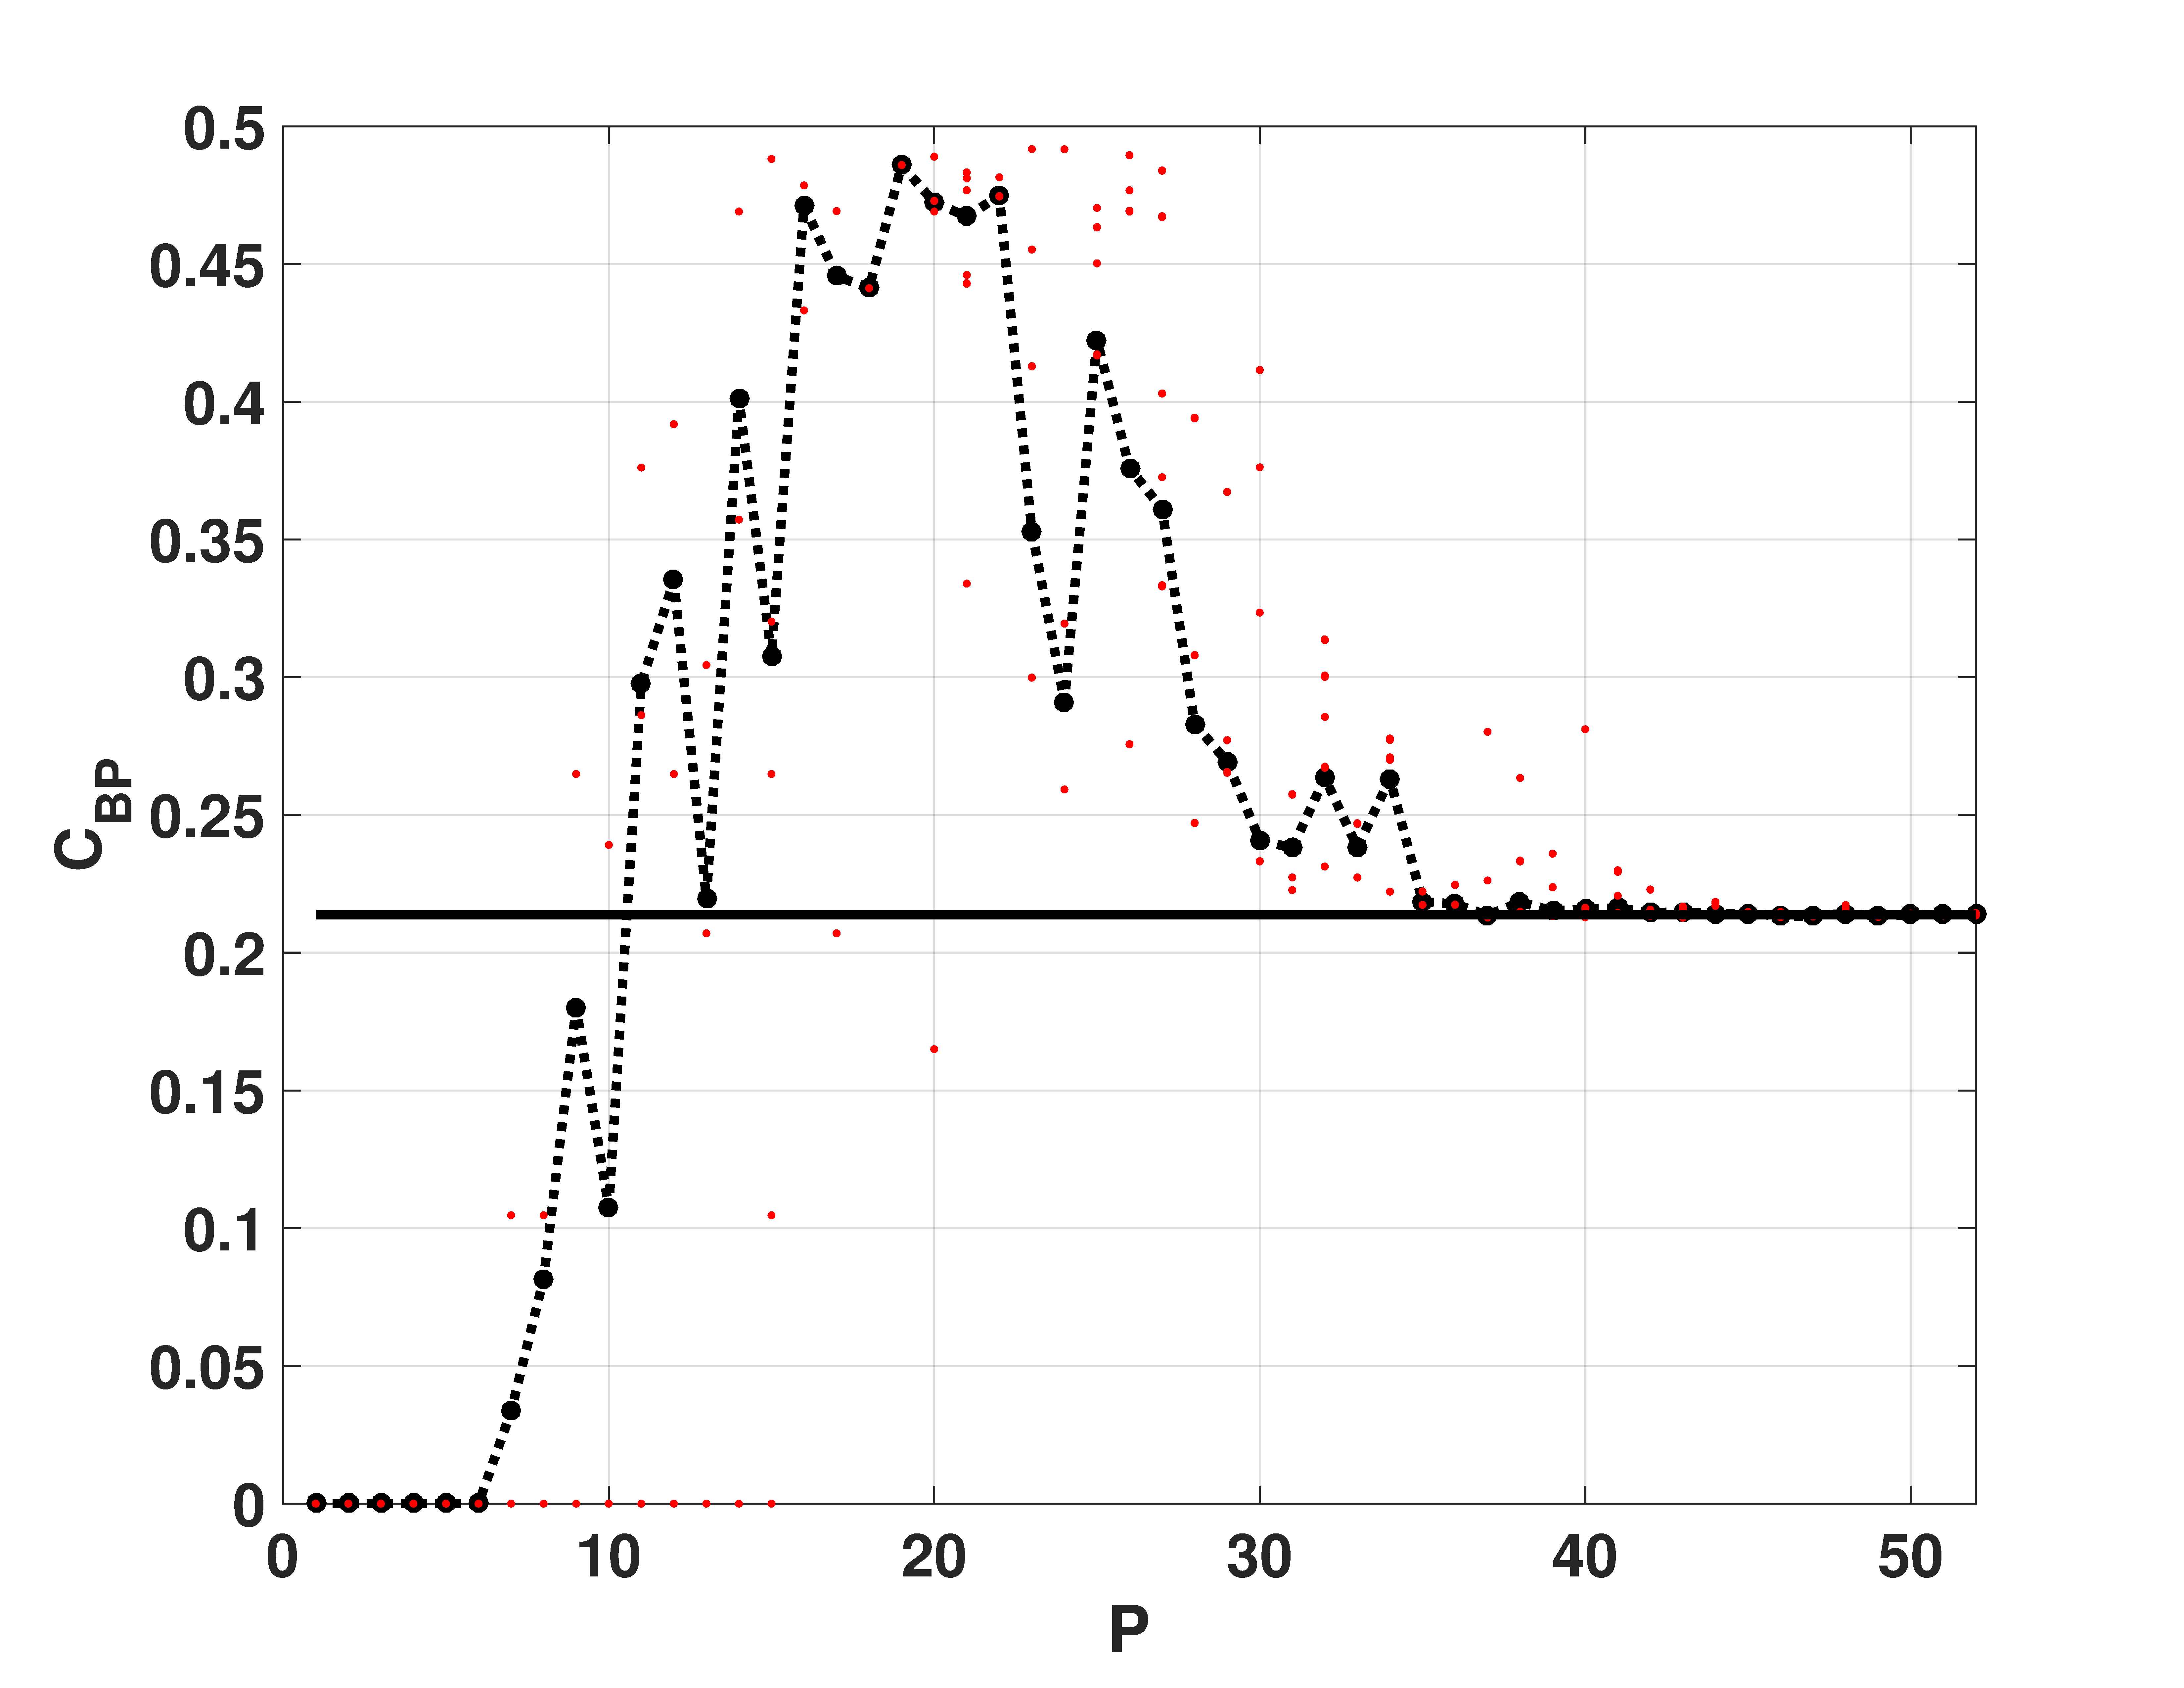
\includegraphics[width=\textwidth]{Cbp_Odd}
		\caption{$C_{BP}$ vs. $B$}
		\label{fig:Cbp_Odd}
	\end{subfigure}
	\begin{subfigure}[b]{0.49\textwidth}
		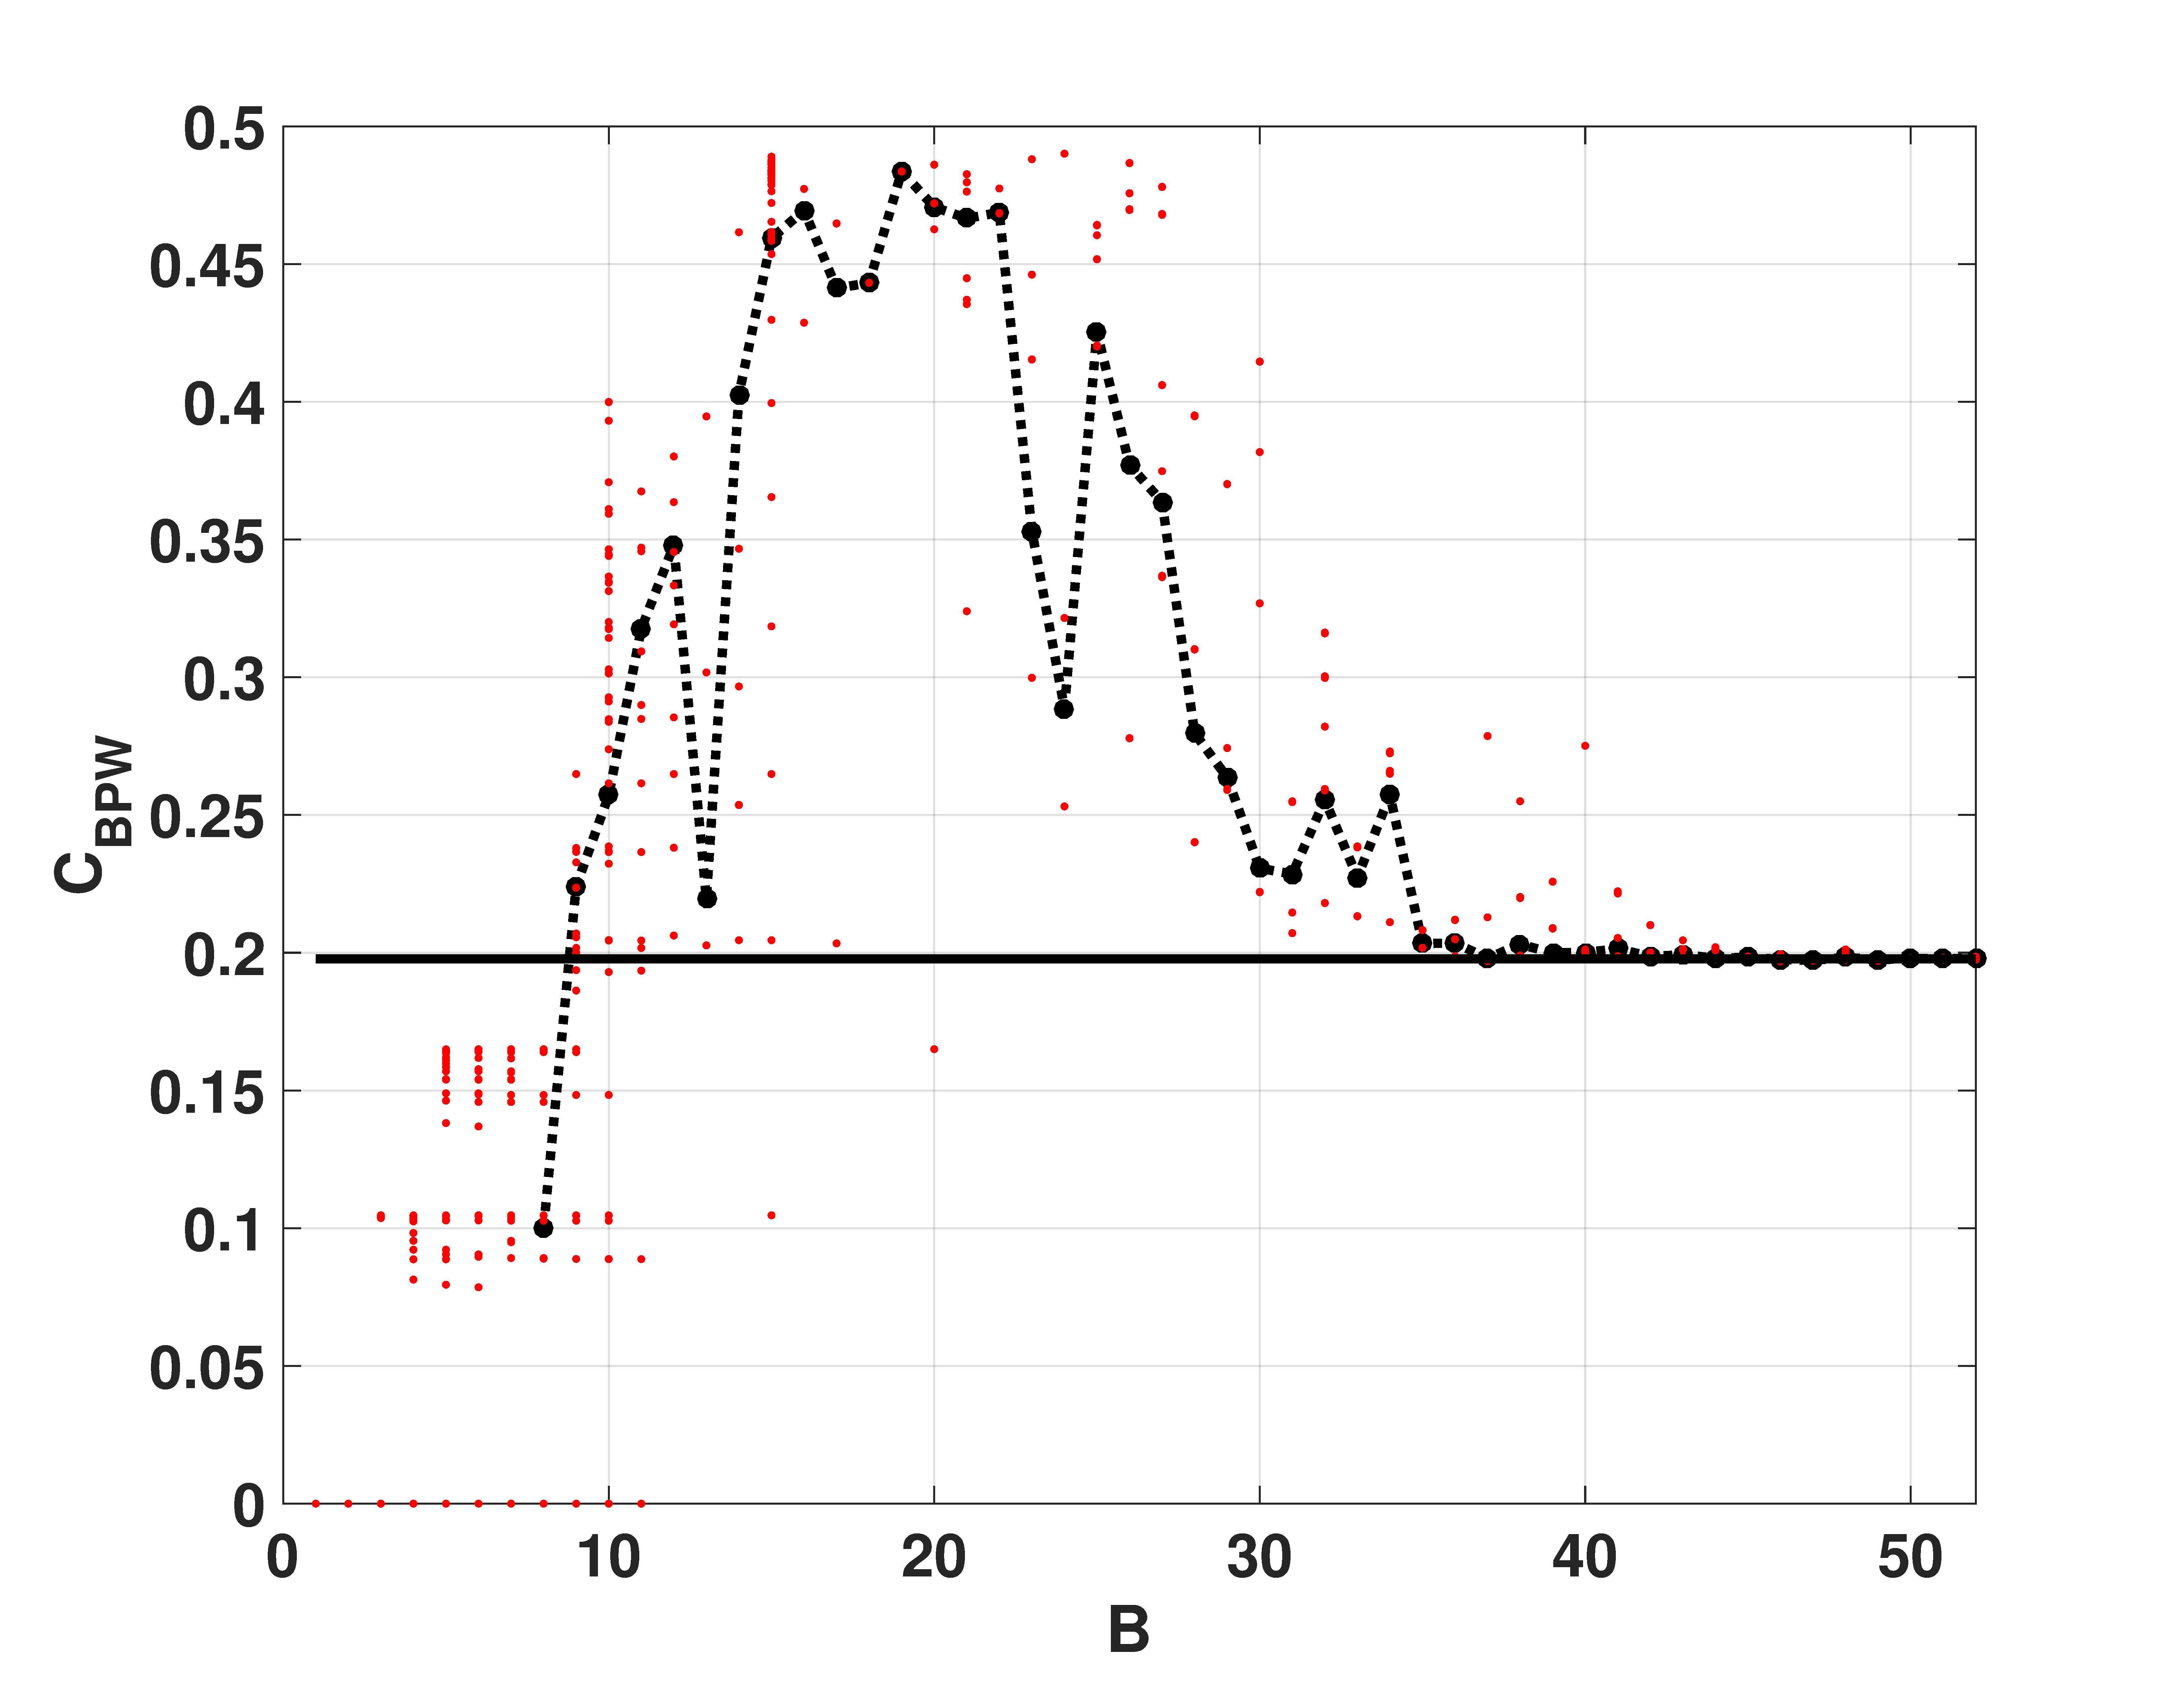
\includegraphics[width=\textwidth]{Cbpw_Odd}
		\caption{$C_{BPW}$ vs. $B$}
		\label{fig:Cbpw_Odd}
	\end{subfigure}
	\begin{subfigure}[b]{0.49\textwidth}
		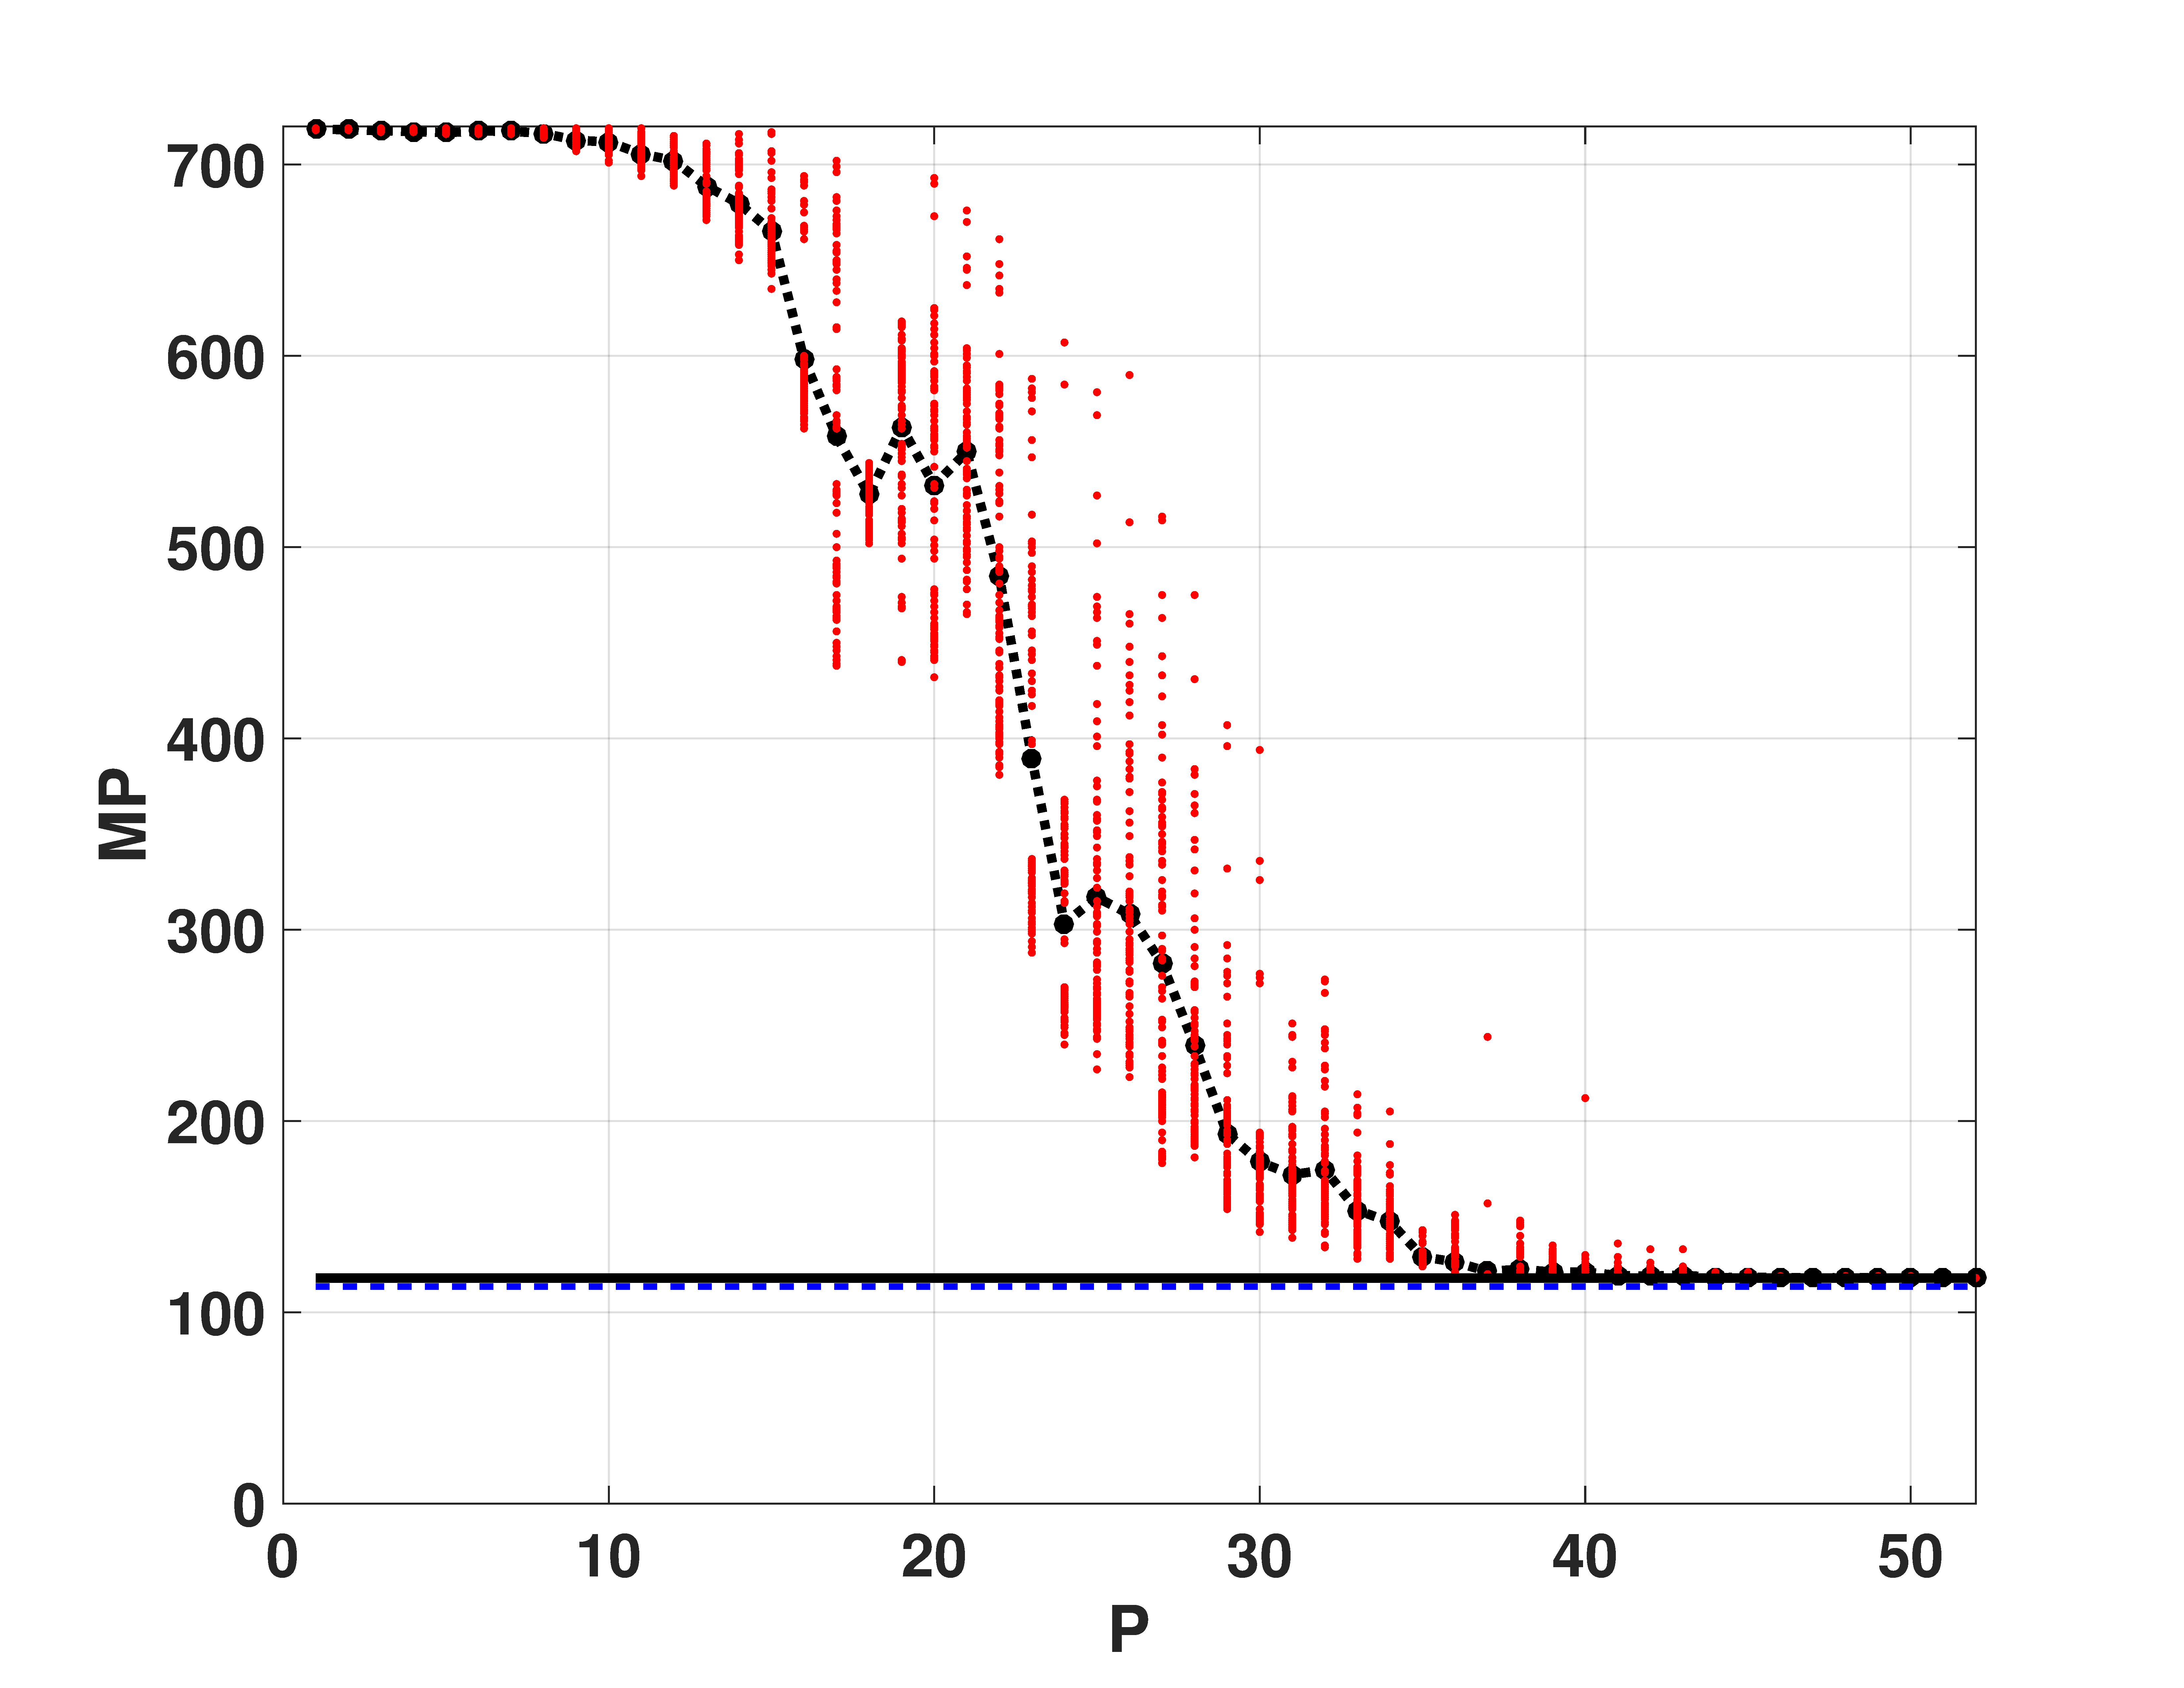
\includegraphics[width=\textwidth]{MP_Odd}
		\caption{MP vs. $B$}
		\label{fig:MP_Odd}
	\end{subfigure}
	\caption{Statistical properties of ODD map.}
	\label{fig:ODD_QuantiB}
\end{figure}

The enhancement showed in Figures \ref{fig:EVEN_QuantiB} and \ref{fig:ODD_QuantiB} is reflected in the position of asymptotic point in the planes \ref{fig:EVEN_HH}, and \ref{fig:ODD_HH}.
In both cases this position is closest to the ideal point $(H_{hist}, H_{BP})=(1, 1)$, because the resulting vectors present better mixing.
%
\begin{figure}[H]
	\centering
	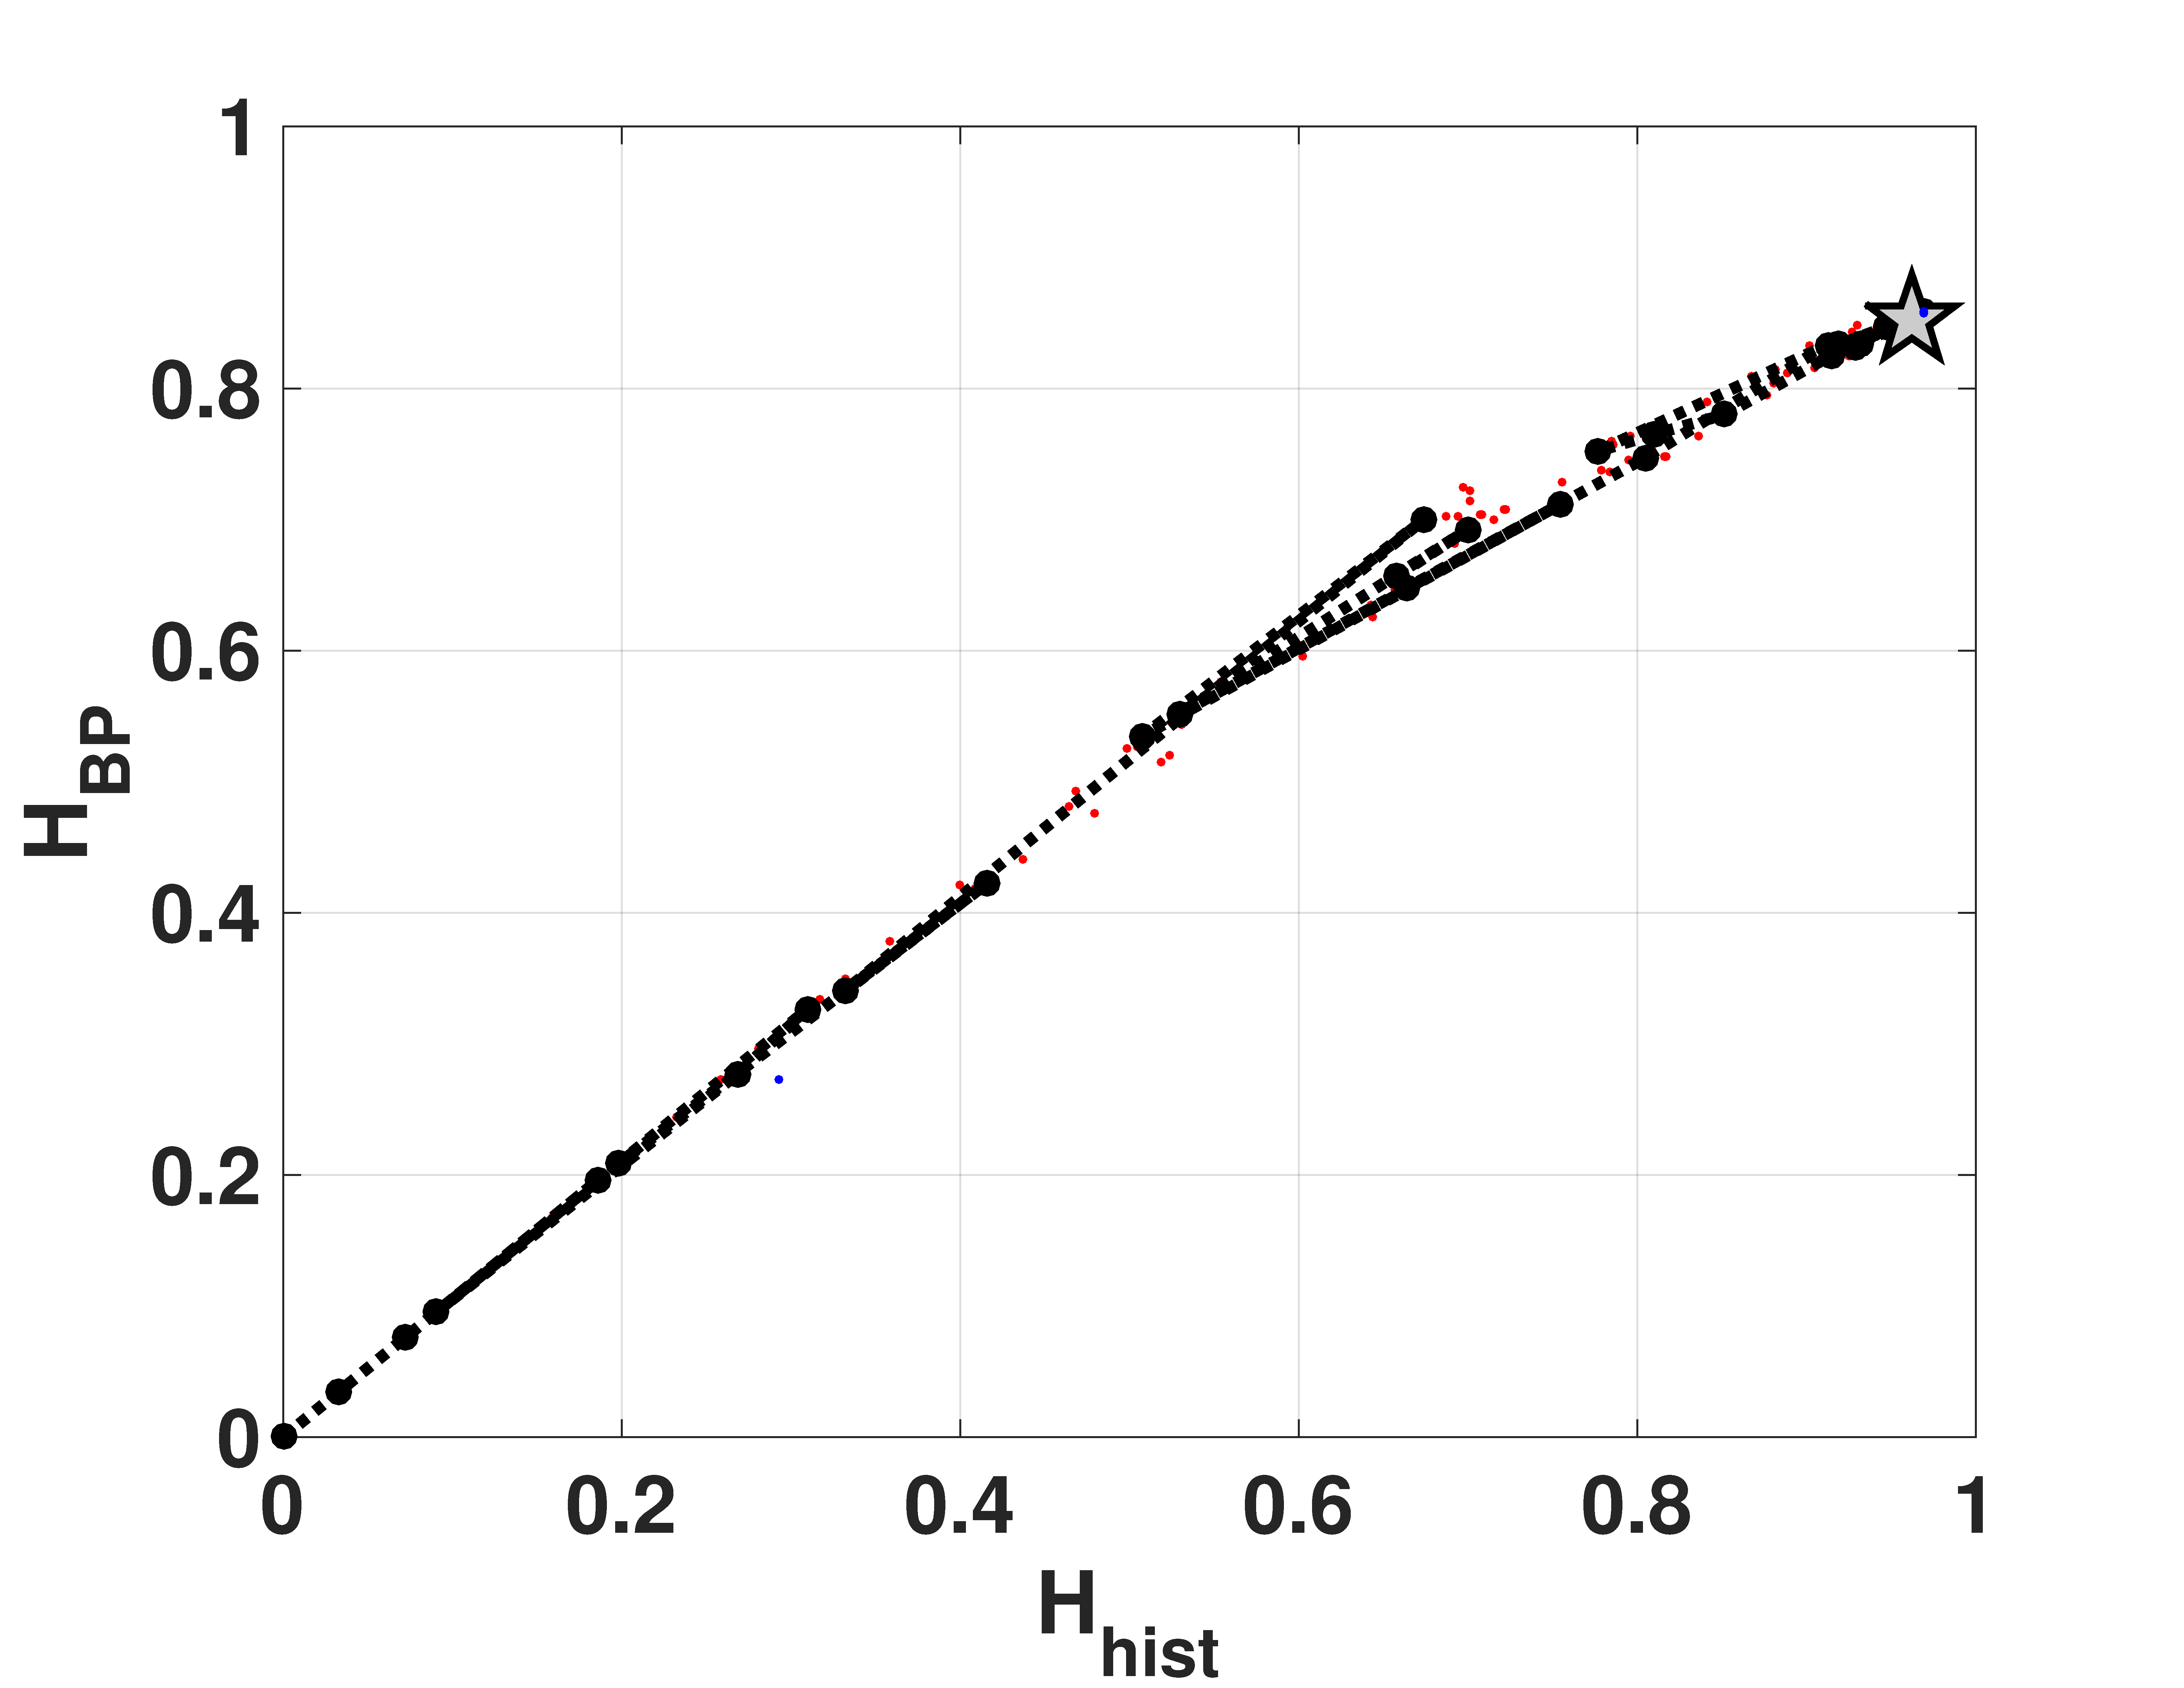
\includegraphics[width=.49\textwidth]{HbpHval_Even}
	\caption{Evolution of statistical properties in double entropy plane for EVEN map $H_{hist} \times H_{BP}$.}
	\label{fig:EVEN_HH}
\end{figure}
%
\begin{figure}[H]
	\centering
	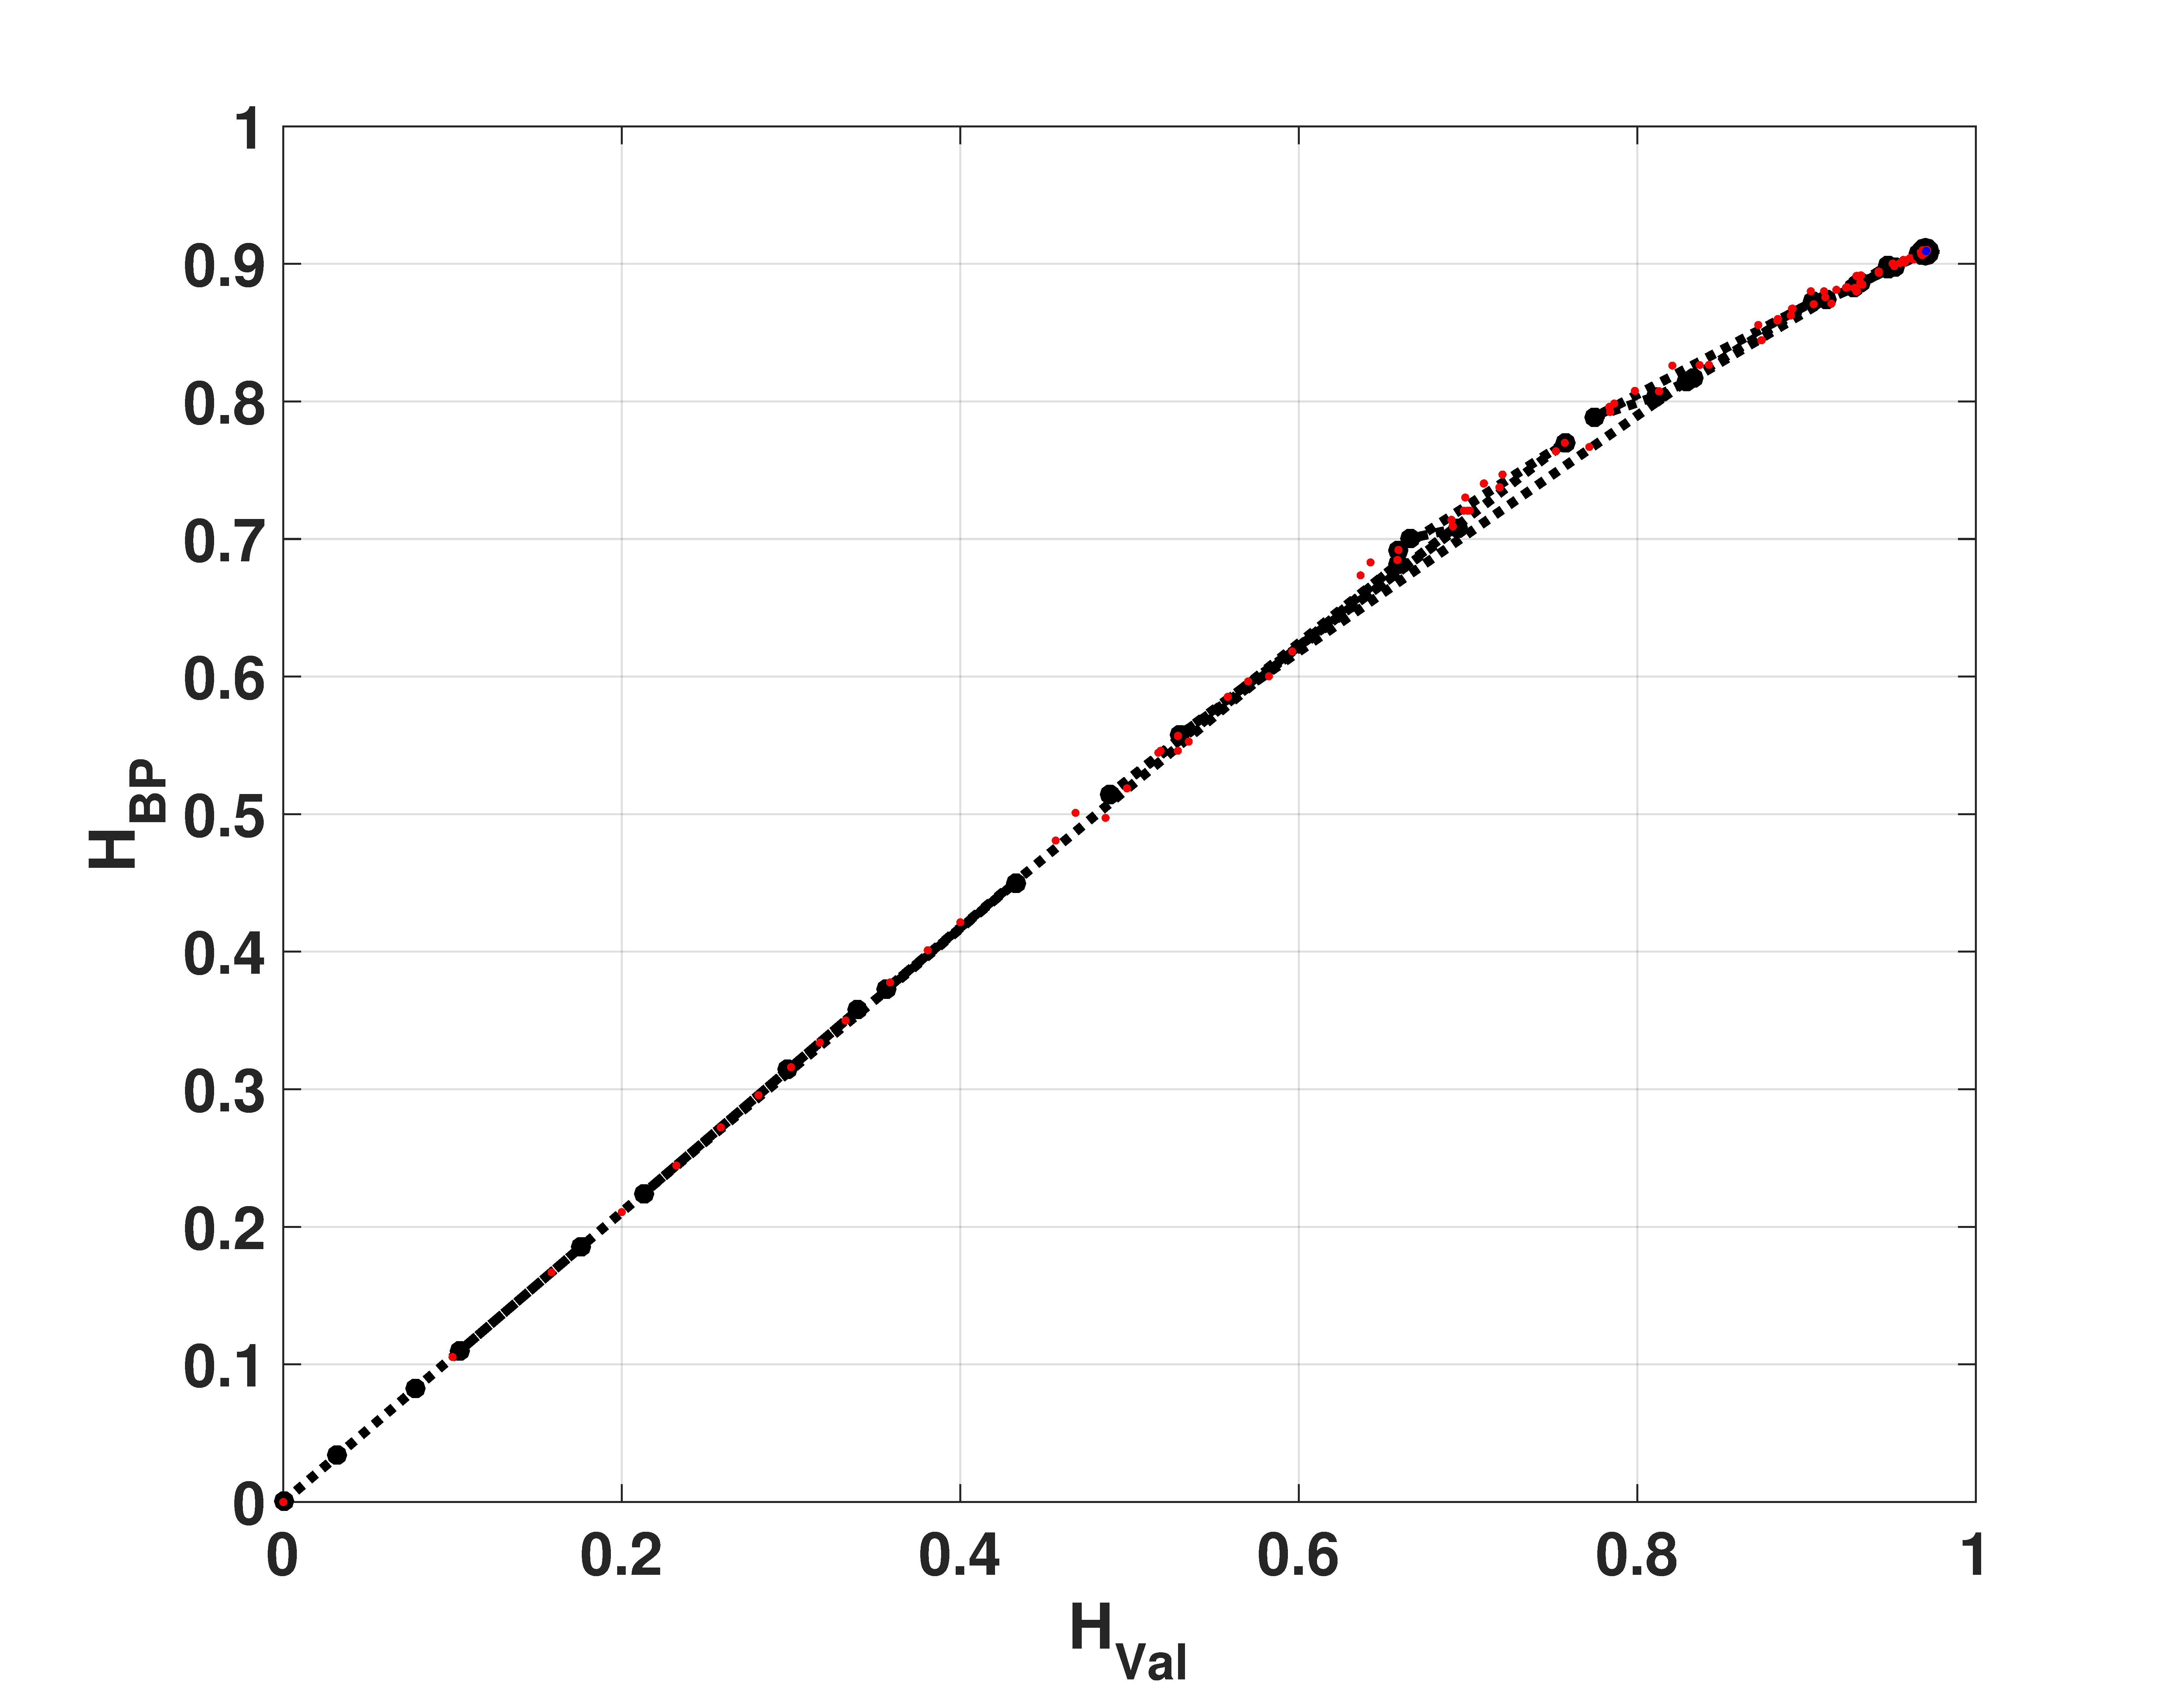
\includegraphics[width=.49\textwidth]{HbpHval_Odd}
	\caption{Evolution of statistical properties in double entropy plane for ODD map $H_{hist} \times H_{BP}$.}
	\label{fig:ODD_HH}
\end{figure}

Compatible results are shown in Figures \ref{fig:EVEN_HC} and \ref{fig:ODD_HC}, the position of asymptotic point is closest to the ideal point $(H_{hist}, H_{BP})=(1, 0)$.
This result reflects that mixing is better because the complexity of resulting system is lower.
This plane detects that the vector generated by ODD skipping is more mixed than EVEN.
%
\begin{figure}[H]
	\centering
	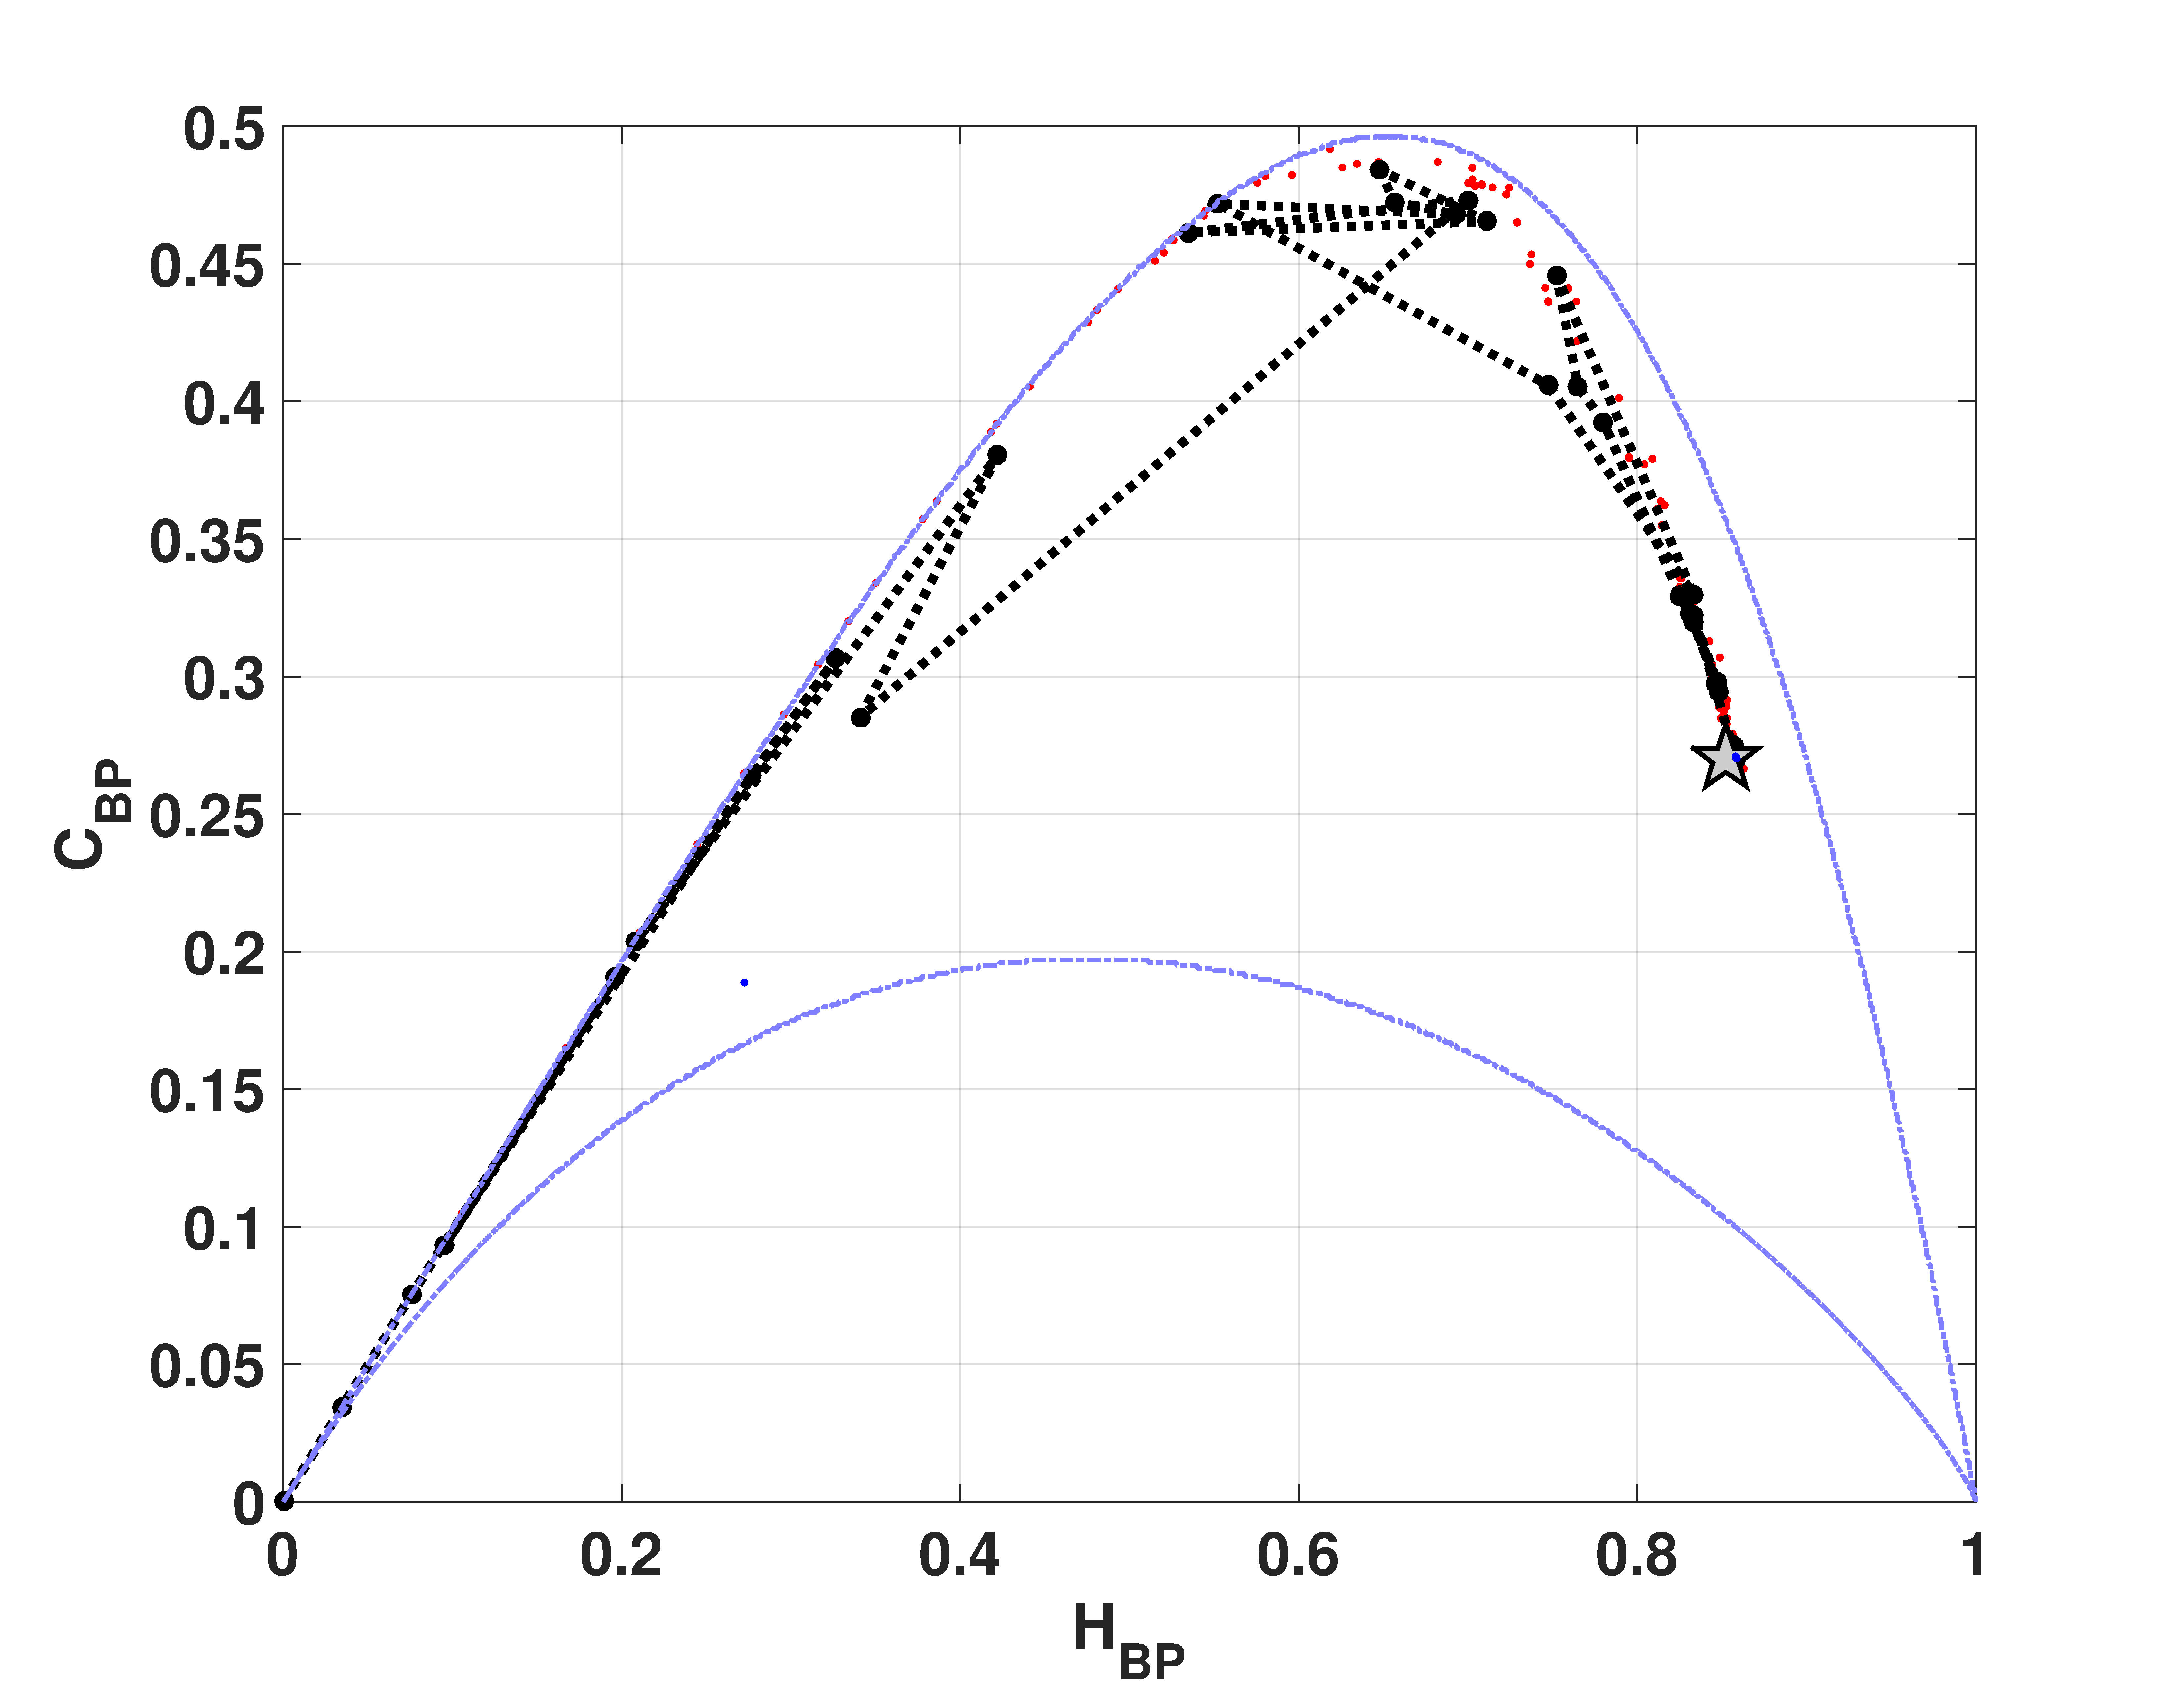
\includegraphics[width=.49\textwidth]{CbpHbp_Even}
	\caption{Evolution of statistical properties in entropy-complexity plane for EVEN map $H_{BP} \times C_{BP}$.}
	\label{fig:EVEN_HC}
\end{figure}
%
\begin{figure}[H]
	\centering
	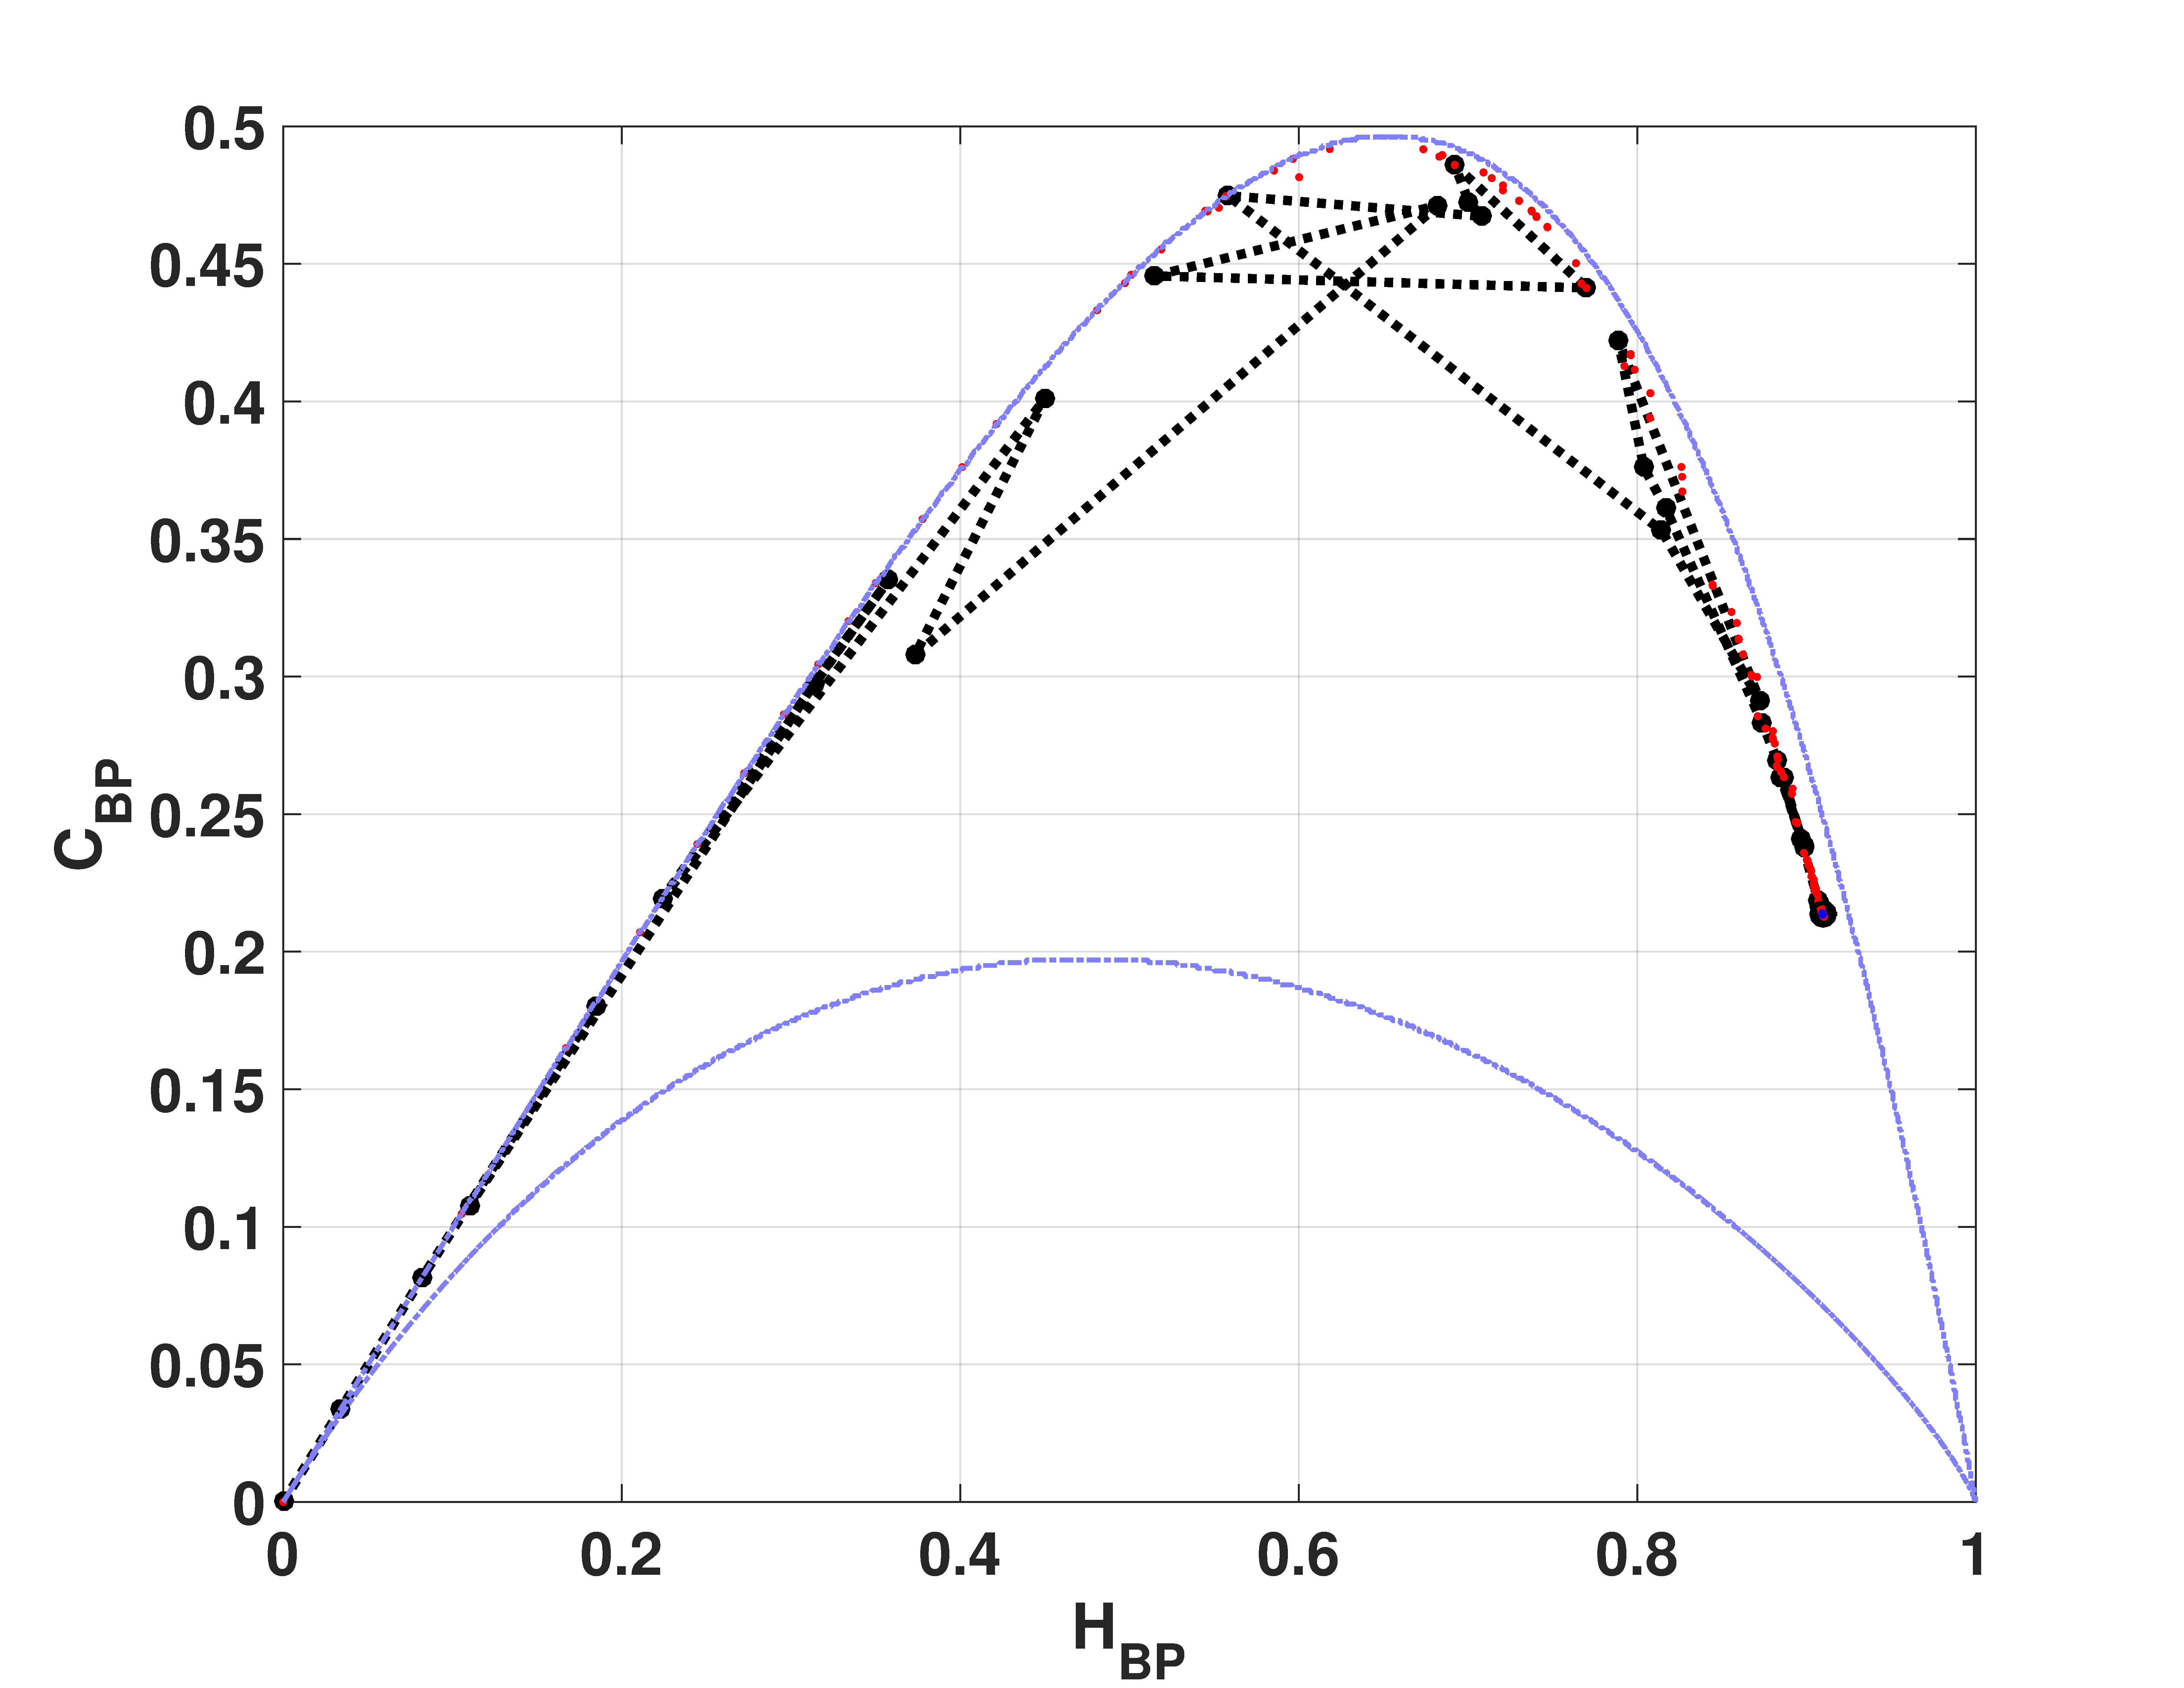
\includegraphics[width=.49\textwidth]{CbpHbp_Odd}
	\caption{Evolution of statistical properties in entropy-complexity plane for ODD map $H_{BP} \times C_{BP}$.}
	\label{fig:ODD_HC}
\end{figure}